% !TEX program = xelatex
% =====================================================================
%  Математик I В — ХЭВЛЭХ ХУВИЛБАР (A4, beamerarticle)
%  Слайдтай яг ижил lectures/lecNN.tex файлаас үүснэ.
%  Нэг лекц хэвлэх бол дугаарыг нь бичнэ (01 ... 16),
%  бүх 16 лекцийг нэг ном болгох бол all гэж бичнэ.
% =====================================================================
\providecommand*{\LECTURE}{all}

\documentclass[11pt,a4paper,oneside]{book}
\usepackage[noamsthm]{beamerarticle}
\usepackage[margin=2.2cm]{geometry}
\definecolor{mathblue}{RGB}{0,82,155}
\definecolor{mathred}{RGB}{178,34,34}
\definecolor{mathgreen}{RGB}{0,120,60}
\definecolor{mathgray}{RGB}{90,90,90}
\usepackage{hyperref}
\hypersetup{colorlinks=true,linkcolor=black,urlcolor=mathblue}

% =====================================================================
%  Математик I В — слайд ба хэвлэх хувилбарт хуваалцах преамбл
%  slides.tex (beamer) ба print.tex (book + beamerarticle) хоёулаа \input хийнэ.
%  \mode<presentation>{...} зөвхөн слайдад, \mode<article>{...} зөвхөн хэвлэхэд.
%  XeLaTeX-ээр хөрвүүлнэ (Overleaf: Menu -> Compiler -> XeLaTeX; latexmkrc үүнийг
%  автоматаар тохируулна).
% =====================================================================

% ---------- Хэл ба фонт ----------
\usepackage{fontspec}
\defaultfontfeatures{Ligatures=TeX}
\usepackage{polyglossia}
\setdefaultlanguage{mongolian}
\setotherlanguage{english}

% Фонтууд TeX Live-д (тиймээс Overleaf-д) байдаг файлуудаас ачаалагдана.
% Слайд: Noto Sans (дэлгэц дээр тод уншигдана); хэвлэх: CMU Serif (Computer Modern-ийн
% кирилл хувилбар, томьёотой нэг загвартай).
\newcommand{\MathSansNoto}{%
  \setsansfont{NotoSans}[Extension=.ttf, UprightFont=*-Regular, BoldFont=*-Bold,
    ItalicFont=*-Italic, BoldItalicFont=*-BoldItalic]%
  \newfontfamily\cyrillicfontsf{NotoSans}[Extension=.ttf, UprightFont=*-Regular,
    BoldFont=*-Bold, ItalicFont=*-Italic, BoldItalicFont=*-BoldItalic]}
\newcommand{\MathSansCMU}{%
  \setsansfont{cmunss.otf}[BoldFont=cmunsx.otf, ItalicFont=cmunsi.otf, BoldItalicFont=cmunso.otf]%
  \newfontfamily\cyrillicfontsf{cmunss.otf}[BoldFont=cmunsx.otf, ItalicFont=cmunsi.otf,
    BoldItalicFont=cmunso.otf]}
\setmainfont{cmunrm.otf}[BoldFont=cmunbx.otf, ItalicFont=cmunti.otf, BoldItalicFont=cmunbi.otf]
\newfontfamily\cyrillicfont{cmunrm.otf}[BoldFont=cmunbx.otf, ItalicFont=cmunti.otf,
  BoldItalicFont=cmunbi.otf]
\setmonofont{cmuntt.otf}[BoldFont=cmuntb.otf, ItalicFont=cmunit.otf, BoldItalicFont=cmuntx.otf]
\newfontfamily\cyrillicfonttt{cmuntt.otf}[BoldFont=cmuntb.otf, ItalicFont=cmunit.otf,
  BoldItalicFont=cmuntx.otf]
\mode<presentation>{\IfFontExistsTF{NotoSans-Regular.ttf}{\MathSansNoto}{\MathSansCMU}}
\mode<article>{\MathSansCMU}

% ---------- Багцууд ----------
\usepackage{amsmath,mathtools,amssymb,amsfonts}
\mode<article>{\usepackage{amsthm}}
\usepackage{mathrsfs}
\usepackage{newunicodechar}
\usepackage{enumitem}
\usepackage{multicol}
\usepackage{environ}
\usepackage{tikz}
\usetikzlibrary{arrows,arrows.meta,calc,patterns,decorations.pathreplacing,positioning}
\usepackage{pgfplots}
\pgfplotsset{compat=1.18}
\usepackage[export]{adjustbox}
\graphicspath{{pictures/}}

% Зураг/хүснэгт хуудсанд (слайдад) багтахгүй бол л жижигрүүлнэ
\mode<presentation>{\newenvironment{fitbox}{\adjustbox{max width=\linewidth,max totalheight=.68\textheight}\bgroup}{\egroup}}
\mode<article>{\newenvironment{fitbox}{\adjustbox{max width=\linewidth,max totalheight=.85\textheight}\bgroup}{\egroup}}
% Слайдад олон баганыг нэг багана болгоно: allowframebreaks зөвхөн нэг баганыг
% хуудас хооронд таслаж чадна. Хэвлэх хувилбарт multicols хэвээр.
\mode<presentation>{\RenewDocumentEnvironment{multicols}{m o o}{}{}}

% Эх файлд шууд бичигдсэн Юникод тэмдэгтүүд
\newunicodechar{→}{\ensuremath{\to}}
\newunicodechar{⇔}{\ensuremath{\Leftrightarrow}}
\newunicodechar{∞}{\ensuremath{\infty}}

% beamer-ийн itemize/enumerate загварыг enumitem эвдэхгүй байлгах
\mode<presentation>{\setlist{label*=\usebeamertemplate{itemize item}}
  \setlist[enumerate]{label=\arabic*.}
  \setlist[enumerate,2]{label=\alph*)}
  \setlist{topsep=2pt,itemsep=2pt,leftmargin=1.5em}}
\mode<article>{\setlist[itemize]{topsep=3pt,itemsep=3pt,leftmargin=1.3em}
  \setlist[enumerate]{topsep=4pt,itemsep=4pt,leftmargin=1.6em}}

% ---------- Макро ----------
\newcommand{\coursename}{Нэг хувьсагчийн функцийн онол 1В (MATH102)}
\newcommand{\semester}{2026 оны намар}
\newcommand{\smallbigcup}{\mathop{\textstyle\bigcup}}
\newcommand{\smallbigcap}{\mathop{\textstyle\bigcap}}
\newcommand{\N}{\mathbb{N}}
\newcommand{\Z}{\mathbb{Z}}
\newcommand{\Q}{\mathbb{Q}}
\newcommand{\R}{\mathbb{R}}
\newcommand{\Sx}{\mathrm{S}}
\newcommand{\itcol}[1]{{\itshape\textcolor{red}{#1}}}
\newcommand{\arccot}{\mathbf{arccot}}
\providecommand{\tg}{\operatorname{tg}}
\providecommand{\ctg}{\operatorname{ctg}}
\providecommand{\arctg}{\operatorname{arctg}}
\providecommand{\arcctg}{\operatorname{arcctg}}

% ---------- Теорем маягийн орчнууд ----------
% beamer-ийн \note (илтгэгчийн тэмдэглэл) командыг "Санамж" орчноор солино
\let\note\relax\let\endnote\relax
\mode<article>{%
  \newtheorem{theorem}{Теорем}[chapter]
  \newtheorem{proposition}{Өгүүлбэр}[chapter]
  \newtheorem{lemma}{Лемма}[section]
  \theoremstyle{definition}
  \newtheorem{definition}{Тодорхойлолт}[chapter]
  \newtheorem{example}{Жишээ}[chapter]
  \theoremstyle{remark}
  \newtheorem*{remark}{Тэмдэглэл}
  \newtheorem*{prof}{Баталгаа}
  \newtheorem*{note}{Санамж}
  \newtheorem*{cor}{Мөрдөлгөө}
  \renewcommand{\proofname}{Баталгаа}}
% Слайдад хайрцаггүй (allowframebreaks хуудас хооронд таслах боломжтой) хувилбар
\mode<presentation>{%
  \newcommand{\MathEnv}[4]{% #1 орчин, #2 нэр, #3 өнгө, #4 дугаартай эсэх (1/0)
    \ifnum#4=1 \newcounter{#1}\fi
    \newenvironment{#1}[1][]{%
      \par\medskip
      \ifnum#4=1 \refstepcounter{#1}\fi
      \begin{trivlist}\item[\hskip\labelsep{\color{#3}\bfseries #2\ifnum#4=1~\thechapter.\arabic{#1}\fi.%
        \if\relax\detokenize{##1}\relax\else\ (##1)\fi}]\ignorespaces}%
      {\end{trivlist}\par\medskip}}
  \newcounter{chapter}
  \MathEnv{theorem}{Теорем}{mathred}{1}
  \MathEnv{proposition}{Өгүүлбэр}{mathred}{1}
  \MathEnv{lemma}{Лемма}{mathred}{1}
  \MathEnv{definition}{Тодорхойлолт}{mathblue}{1}
  \MathEnv{example}{Жишээ}{mathgreen}{1}
  \MathEnv{remark}{Тэмдэглэл}{mathgray}{0}
  \MathEnv{note}{Санамж}{mathgray}{0}
  \MathEnv{cor}{Мөрдөлгөө}{mathred}{0}
  \newenvironment{prof}[1][]{\par\smallskip\begin{trivlist}\item[\hskip\labelsep{\itshape Баталгаа.}]\ignorespaces}%
    {\hfill$\square$\end{trivlist}\par\medskip}
  \providecommand{\qedhere}{}
  \providecommand{\paragraph}{}
  \renewcommand{\paragraph}[1]{\par\medskip\noindent{\bfseries #1}\enskip}
  \let\proof\relax\let\endproof\relax
  \newenvironment{proof}[1][]{\begin{prof}}{\end{prof}}}

% Бодлого ба бодолт
\newcounter{problem}
\newenvironment{problem}[1][]{\refstepcounter{problem}\par\noindent\textbf{Бодлого~\theproblem.}~#1}{\par}
\newif\ifshowsolutions
\showsolutionstrue   % бодолтыг нуух бол \showsolutionsfalse
\NewEnviron{solution}{\ifshowsolutions\par\smallskip\noindent\textit{Бодолт. }\BODY\par\smallskip\fi}


% ---------- Семинар ба гэрийн даалгаврын бодлогууд (Г.Н. Берман) ----------
% \ProblemSet{Семинар 10}  -> шинэ хэсэг, дугаарлалт 1-ээс
% \pgroup{заавар}          -> бүлэг бодлогын заавар
% \begin{plist} \prob{936}{$x=a\cos t$} \end{plist}  -> [Б.936] нь Берманы дугаар
\newcounter{pnum}
\mode<presentation>{\newcommand{\ProblemSet}[1]{\setcounter{pnum}{0}\section{#1}}}
\mode<article>{\newcommand{\ProblemSet}[1]{\setcounter{pnum}{0}\section*{#1}\addcontentsline{toc}{section}{#1}}}
\newcommand{\bn}[1]{\hfill{\color{mathgray}\scriptsize[Б.#1]}}
\newcommand{\prob}[2]{\stepcounter{pnum}\item[\textbf{\thepnum.}] #2\bn{#1}}
\newcommand{\pgroup}[1]{\par\smallskip\noindent\textbf{#1}\par}
\mode<presentation>{\newenvironment{plist}{\begin{enumerate}[leftmargin=2.2em,itemsep=3pt]}{\end{enumerate}}}
\mode<article>{\newenvironment{plist}{\begin{multicols}{2}\begin{enumerate}[leftmargin=2.2em,itemsep=2pt]}{\end{enumerate}\end{multicols}}}

% ---------- Лекцийн гарчиг ----------
% \MathLecture{дугаар}{гарчиг}: слайдад гарчгийн хуудас, хэвлэхэд \chapter
\newcommand{\MathLecture}[2]{%
  \setcounter{chapter}{\numexpr#1-1\relax}%
  \mode<article>{\chapter{#2}}%
  \mode<presentation>{\stepcounter{chapter}%
    \setcounter{definition}{0}\setcounter{theorem}{0}\setcounter{example}{0}%
    \setcounter{proposition}{0}\setcounter{lemma}{0}%
    \title[Лекц #1]{Лекц #1. #2}\subtitle{\coursename}\date{\semester}%
    \begin{frame}[plain]\titlepage\end{frame}%
    \begin{frame}{Агуулга}\tableofcontents\end{frame}}}

% Хэвлэхэд frame-ийн гарчиг давхардахгүй (бүлэг, дэд бүлгийн гарчиг хангалттай)
\setbeamertemplate{frametitle}{}
% "Бүлэг" биш "Лекц" гэж гарна
\gappto\captionsmongolian{\renewcommand{\chaptername}{Лекц}}

\begin{document}
\def\ALL{all}
\ifx\LECTURE\ALL
  \title{Математик I В\\[4pt]\large\coursename}
  \author{МУИС, Математикийн тэнхим}
  \date{\semester}
  \maketitle
  \tableofcontents
  % Лекц 1. Хэллэг ба Логик, Үнэний хүснэгт
% Эх: latex/lectures/lec01-logic.tex (scripts/latex_to_beamer.py-ээр хөрвүүлсэн)
% Frame бүр слайдад нэг (эсвэл allowframebreaks-аар хэд хэдэн) хуудас болно;
% хэвлэх хувилбарт frame-ийн хил харагдахгүй, текст үргэлжилсэн байна.

\MathLecture{1}{Хэллэг ба Логик, Үнэний хүснэгт}

\section*{Лекцийн зорилго}
\begin{frame}[allowframebreaks]{Лекцийн зорилго}
\begin{itemize}
  \item Логик, хэллэгийн үндсэн ойлголтыг тодорхойлох.
  \item Үнэний хүснэгтээр логик томьёог шинжлэн үнэнийг тогтоох аргыг эзэмшүүлэх.
  \item Баталгааны үндсэн аргуудыг тодорхойлолт бүрээр нь жишээтэй тайлбарлах.
  \item Олонлог, түүн дээрх үйлдлүүд
\end{itemize}
Цаашид хэрэглэгдэх тэмдэглэгээнүүд\\
\begin{multicols}{2}
\begin{enumerate}
\item $\forall$- дурын, аливаа
\item $\exists$- оршин байна, олдоно
\item $\exists!$- цор ганц оршин байна, ганц олдоно 
\item $\Rightarrow$- мөрдөнө, мөрдөн гарна
\item $\in$ - харяалагдна
\item $\notin$- харяалагдахгүй
\item $\Leftrightarrow$- эквивалент, зайлшгүй бөгөөд хүрэлцээтэй
\item $\mathbb{N}$- натурал тоон олонлог
\item $\mathbb{Z}$- бүхэл тоон олонлог
\item $\mathbb{Q}$-рационал тоон олонлог
\item $\mathbb{R}$- бодит тоон олонлог
\end{enumerate}
 Грек үсгүүдийн нэршил\\
\begin{fitbox}\begin{tabular}{c|c|l}
\hline
Том үсэг & Жижиг үсэг & Дуудлага \\ \hline
$A$ & $\alpha$ & альфа \\
$B$ & $\beta$ & бета \\
$\Gamma$ & $\gamma$ & гамма \\
$\Delta$ & $\delta$ & дельта \\
$E$ & $\epsilon$ & эпсилон \\
$Z$ & $\zeta$ & зета \\
$H$ & $\eta$ & эта \\
$\Theta$ & $\theta$ & тета \\
$\Xi$ & $\xi$ & кси \\
$\Lambda$ & $\lambda$ & лямбда \\
$M$ & $\mu$ & мю \\
$N$ & $\nu$ & ню \\
$\Sigma$ & $\sigma$ & сигма \\
$T$ & $\tau$ & тау \\
$\Phi$ & $\varphi$ & фи \\
$\Psi$ & $\psi$ & пси  \\
\hline
\end{tabular}\end{fitbox}
\end{multicols}
\end{frame}

\begin{frame}[allowframebreaks]{Лекцийн зорилго}
\begin{remark}
     $\forall$, $\exists$, $\exists!$, $\Rightarrow$, $\in$, $\Leftrightarrow$ тэмдэгүүдийг квантор гэж нэрлэдэг.
\end{remark}
\end{frame}

\begin{frame}[allowframebreaks]{Лекцийн зорилго}
\begin{example} Логик хэллэгийн уншилтын жишээ
  \begin{enumerate} 
      \item
\[
\forall x\in\mathbb{R} \text{ бол } \big( x>1  \Rightarrow  x^2>1 \big).
\]
\textit{Уншилт:} Бүх бодит \(x\)-ийн хувьд, хэрэв \(x>1\) бол \(x^2>1\).\par\medskip
      \item \[
\exists!\,n\in\mathbb{N}\, , \,\big( n^2=25\big).
\]
\textit{Уншилт:} Натурал тоонууд дундаас \(n^2=25\) байх \emph{цор ганц} \(n\) (өөрөөр хэлбэл \(n=5\)) оршин байна.\par\medskip
      \item\[
\forall n\in\mathbb{Z}\ \text{ хувьд } \big(n \text{ тэгш}\big)\ \Leftrightarrow\ \big(\exists k\in\mathbb{Z}\ n=2k\big).
\]
\textit{Уншилт:} Бүх бүхэл \(n\)-ийн хувьд, \(n\) тэгш байх \emph{зайлшгүй бөгөөд хүрэлцээтэй нөхцөл} нь зарим бүхэл \(k\) тооны хувьд \(n=2k\) гэж бичигдэх нөхцөл болно.\par\medskip
\textit{Өөрөөр хэлбэл :} Бүх бүхэл \(n\)-ийн хувьд, \(n\)  \emph{зөвхөн тэгш байх үед л} зарим бүхэл \(k\) тооны хувьд \(n=2k\) гэж бичигдэх болно.\par\medskip
      \item \[
\forall \epsilon>0\, ,  \exists \delta>0\,  , \forall x\in\mathbb{R}\ 
\Big(|x-1|<\delta\ \Rightarrow\ \big|\tfrac{x^2-1}{x+1}-0\big|<\epsilon\Big).
\]
\textit{Уншилт:} Дурын эерэг \(\epsilon\) тооны хувьд, ямар нэг эерэг \(\delta\) тоо олдох ба түүний хувьд, бүх бодит \(x\)-ийн хувьд \(|x-1|<\delta\) бол
\(\big|\frac{x^2-1}{x+1}\big|<\epsilon\) байна.\par\medskip
  \end{enumerate}  
\end{example}
\end{frame}

\section{Хэллэг ба логик}
\subsection{Хэллэг}
\begin{frame}[allowframebreaks]{Хэллэг}
\begin{definition} \emph{Үнэн эсвэл худал гэдгийг нь нэгэн утгатай тодорхой тогтоож болох} өгүүлбэрийг \textbf{хэллэг} (proposition) гэнэ.
\end{definition}
 Өөрөөр хэлбэл, тухайн хэллэгийн үнэний утга (үнэн/худал) нь хамрах хүрээ, хугацаа, хэрэглэсэн ухагдахуунууд тодорхой үед ганц утгатайгаар тодорхойлогддог хэллэг юм.
\end{frame}

\begin{frame}[allowframebreaks]{Хэллэг}
 \begin{example}
     \begin{itemize}
  \item ``$5<9$'' — үнэн хэллэг.
  \item ``7 нь тэгш.'' — худал хэллэг.
  \item ``$\pi$ нь рационал тоо.'' — худал хэллэг.
  \item ``бүх $x\in\mathbb{R}$ хувьд $x^2\ge 0$ .'' — үнэн хэллэг (квантортой хэллэг).
  \item ``2026 оны 1-р сарын 1-нд МУИС I байрны цэцэрлэгт цас орсон.'' — хугацаа, газар тодорхой тул үнэн эсэхийг тогтоож болно.
\end{itemize}
 \end{example}
\end{frame}

\begin{frame}[allowframebreaks]{Хэллэг}
\begin{remark}
(1) Тушаал, хүсэлт, асуулт гэх мэт нь хэллэг биш: \\
``Хаалгаа хаа!'', \\
``Хаалга хаасан уу?''. \\
(2) \emph{Нээлттэй хэллэг} буюу хувьсагчтай, кванторгүй хэллэг (ж: ``$x>2$'') нь хэллэг биш; \\
харин $\forall x\in\mathbb{R}\,(x>2 \Rightarrow x^2>4)$ шиг квантортой бол хэллэг болно. \\
(3) Дунджаар, ``дулаахан'' гэх мэт тодорхойгүй шалгууртай, контекст тодорхойгүй хэллэгүүд нь хэллэг биш; шалгуур, хэмжүүрийг тодорхой тогтоосноор хэллэг болгож болно.
\end{remark}
\end{frame}

\begin{frame}[allowframebreaks]{Хэллэг}
\begin{definition}
Хэллэг үнэн бол түүнийг 1, худал бол түүнийг 0 утгатай гээд 0 ба 1 утгийг хэллэгийн \textbf{үнэний утга} гэнэ.
\end{definition}
Бид цаашид хэллэгийг үсгээр нэрлэх болно. 
$$P=\{11>9\} \,,\, Q=\{\exists n\in\mathbf{N} ,  \big( n^2=-1\big)\}$$ гэе. Тэгвэл $P$ хэллэг үнэн тул 1, $Q$ хэллэг худал тул 0 утгатай.
\end{frame}

\subsection{Логик холбоосууд}
\begin{frame}[allowframebreaks]{Логик холбоосууд}
Бид олон хэллэгүүдийг нийлүүлэн тэдгээрээс дүгнэлт гаргадаг. Өөрөөр хэлбэл\\ математикийн теорем гэдэг нь нийлмэл хэллэг байдаг. Бид энэ хэсэгт нийлмэл хэллэг хэзээ үнэн байх тухай авч үзнэ. 

Эхлээд нэг эсвэл хэд хэдэн хэллэгээс хэрхэн шинэ хэллэг үүсгэх талаар авч үзье.
\end{frame}

\begin{frame}[allowframebreaks]{Логик холбоосууд}
\begin{definition}[Үгүйсгэл] Зөвхөн $A$ хэллэг худал байхад үнэн байдаг хэллэгийг $\lnot A$ гэж тэмдэглэх ба "$A$ биш" гэсэн хэллэг болно. Үүнийг үгүйсгэл гэнэ. 
\end{definition}
\end{frame}

\begin{frame}[allowframebreaks]{Логик холбоосууд}
\begin{definition}[ Импликаци, “Хэрэв…бол”] Зөвхөн $A$ хэллэг худал байхад эсвэл $B$ хэллэг үнэн байхад үнэн байдаг хэллэгийг $A\Rightarrow B$ гэж тэмдэглэх ба  "$A$ байсан бол $B$  байна" гэсэн хэллэг болно. $B$ хэллэгийг $A$ хэллэгийн мөрдөлгөө гэнэ. Энэ нийлмэл хэллэгээр шалтгаан үр дагаварын холбоог илэрхийлнэ.
\end{definition}
\end{frame}

\begin{frame}[allowframebreaks]{Логик холбоосууд}
\begin{definition}[Үржвэр, "... ба ..."]
$A$ ба $B$ хэллэгүүд хоёул үнэн байхад үнэн байдаг бусад үед худал байдаг  хэллэгийг $A {\text{ ба }} B$ эсвэл $A\land B$ гэж тэмбэглэх ба энэ нь "$A$ ба $B$" гэсэн хэллэг болох ба $A$, $B$ хэллэгүүдийн үржвэр /conjuction / гэдэг. 
\end{definition}
\end{frame}

\begin{frame}[allowframebreaks]{Логик холбоосууд}
\begin{definition}[Нийлбэр, "... эсвэл ..."]
$A$ ба $B$ хэллэгүүдийн ядаж нэг үнэн байхад үнэн байдаг бусад үед худал байдаг хэллэгийг $A\lor B$ гэж тэмдэглэх ба энэ нь $"A {\text{ эсвэл }} B" $  гэсэн хэллэг болох ба $A$, $B$ хэллэгүүдийн  нийлбэр /disjunction / гэдэг. 
\end{definition}
Мөн нь нийлмэл хэллэгийн үнэн-утгыг хувьсагчдын (хэллэгүүдийн) бүх боломжит үнэн худал утгийн хослол бүр дээр системтэйгээр тооцож харуулсан хүснэгтийг нийлмэл хэллэгийн үнэний хүснэгт гэдэг.


$\lnot A$ , $A\lor B$, $A\land B$ , $A\Rightarrow B$ үзэгдлүүдийн үнэний хүснэгтийг хийж үзье. \\
\begin{center}\begin{fitbox}\begin{tabular}{|c|c|c|c|c|c|}
\hline
$A$&$B$&$\lnot A$&$A\lor B$&$A\land B$&$A\Rightarrow B$\\
\hline
1&1&0&1&1&1\\
\hline
1&0&0&1&0&0\\
\hline
0&1&1&1&0&1\\
\hline
0&0&1&0&0&1\\
\hline
\end{tabular}\end{fitbox}\end{center}
\end{frame}

\begin{frame}[allowframebreaks]{Логик холбоосууд}
\begin{example}
$$A=\{{\text{Бороо орсон}}\}$$
$$B=\{{\text{Газар нойтон байна}}\}$$ гэсэн хэллэгүүдийг авч үзье. 
\begin{itemize}
\item $\lnot A=\{{\text{Бороо ороогүй}}\}$\\
Энэ хэллэг $A$ тай яг эсрэг байна.
\item $A\lor B=\{{\text{Бороо орсон эсвэл Газар нойтон байна}}\}$\\
Энэ нийлмэл хэллэгт орсон 2 хэллэгийн ядаж 1 нь үнэн үед $A\lor B$-г үнэн гэж үзнэ. Өөрөөр хэлбэл "Бороо орсон боловч газар хуурай байсан ч", "Бороо ороогүйч газар нойтон байсан ч", "Бороо ороод газар нойтон байсан ч" "$A$ эсвэл $B$" хэллэг үнэн байна. 
\begin{remark}
    Нөхцөл $A$ худал үед $A\Rightarrow B$ үргэлж үнэн гэж үздэг. 
    
    Жишээ: ``Хэрэв би өнөөдөр ирвэл (A) амттан авна (B).'' Би ирээгүй (A худал) бол амттан авсан/аваагүйгээс үл хамааран хэллэгийг худал болгох шалтгаан байхгүй тул нийт хэллэг үнэн гэж тооцно.
\end{remark}
\item $A\land B=\{{\text{Бороо орсон ба Газар нойтон байна}}\}$\\
Энэ нийлмэл хэллэгт орсон 2 хэллэг 2-уул үнэн үед $A\land B$-г үнэн гэж үзнэ. Өөрөөр хэлбэл "Бороо орсон бас газар нойтон" байсан үед л үнэн бусад үед худал гэж үзнэ.
\item $(A\Rightarrow B)=\{{\text{Бороо орсон бол Газар нойтон байна}}\}$\\
Энэ нийлмэл хэллэгт Бороо орсон нь шалтгаан,   Газар нойтон байх нь үр дүн юм. Энэ хэллэг нь "Бороо орсон бас   Газар нойтон биш" байхад л худал, бусад үед үнэн гэж үзнэ. 
\end{itemize}
\end{example}
\end{frame}

\begin{frame}[allowframebreaks]{Логик холбоосууд}
\begin{definition}[Эквивалент, if and only if] 
$A\Rightarrow B$ мөн $B\Rightarrow A$ бол $A$ ба $B$-г эквивалент  /ижил/ хэллэгүүд ба $A$-г $B$-ийн зайлашгүй бөгөөд хүрэлцээтэй нөхцөл гээд $A\Leftrightarrow B$ гэж тэмдэглэнэ. 
\end{definition} 
$A\Leftrightarrow B$ бол $A$ болон $B$ хэллэгүүд ижил үнэний утгатай мөн ижил ижил үнэний утгатай бол $A\Leftrightarrow B$ байна. 
\end{frame}

\begin{frame}[allowframebreaks]{Логик холбоосууд}
\begin{example}
$x=2\Rightarrow x^2=4$ хэллэг үнэн.\\
$x^2=4\Rightarrow x=-2$ хэллэг худал.\\
$x+5=y+3\Leftrightarrow x+2=y$ хэллэг үнэн. \\
$\{n>10$ ба $n<12 {\text{ бүхэл тоо}}\}\Leftrightarrow \{n=11\}$\\
$\{n\leq 10$ эсвэл $n\geq 12 {\text{ бүхэл тоо}}\}\Leftrightarrow \{n\neq 11\}$\\
\end{example}
\end{frame}

\subsection{Логикийн хуулиуд, тавтологи ба зөрчил}
\begin{frame}[allowframebreaks]{Логикийн хуулиуд, тавтологи ба зөрчил}
\begin{definition}[Тавтологи] Ямагт үнэн байдаг хэллэгийг тавтологи гэнэ.
\end{definition}
\end{frame}

\begin{frame}[allowframebreaks]{Логикийн хуулиуд, тавтологи ба зөрчил}
\begin{definition}[Зөрчил]
    Ямагт худал байдаг хэллэгийг зөрчил гэнэ.
\end{definition}
\end{frame}

\begin{frame}[allowframebreaks]{Логикийн хуулиуд, тавтологи ба зөрчил}
\begin{definition}[Баталгаа]
Өгөгдсөн суурь өгүүлбэрүүдээс (аксиом, тодорхойлолт, өмнө батлагдсан хэллэгүүдээс) \emph{логикийн дүгнэлтийн дүрмүүд}-ийг ($\land$, $\lor$, $\Rightarrow$, $\lnot$, $\Leftrightarrow$ гэх мэт) хэрэглэн зорьсон дүгнэлтэд хүрэх төгсгөлөг алхамуудын дараалалыг баталгаа гэнэ. Алхам бүр нь 

(i) суурь өгүүлбэр, эсвэл 
(ii) өмнөх мөрүүдээс дүрмээр гарсан шинэ өгүүлбэр байна.
\end{definition}
\end{frame}

\begin{frame}[allowframebreaks]{Логикийн хуулиуд, тавтологи ба зөрчил}
\begin{definition}[Tеорем]
Аксиом, тодорхойлолт, өмнө батлагдсан хэллэгүүдээс логикийн зөв дүгнэлтийн дүрмүүдийг ашиглан төгсгөлөг \emph{алхамчилсан баталгаагаар} гаргаж авсан үнэн хэллэгийг теорем гэнэ.
\end{definition}
 Теорем нь ерөнхийдөө “Хэрэв (нөхцөлүүд) бол (дүгнэлт)” хэлбэртэй байна.
\end{frame}

\begin{frame}[allowframebreaks]{Логикийн хуулиуд, тавтологи ба зөрчил}
\begin{example}
   Теорем.  Хэрэв $P$ хэллэг бол $Q=P\lor\lnot P$ хэллэг тавтологи байна.

   Баталгаа.  $Q=P\lor\lnot P$ хэллэгийн үнэний хүснэгтийг байгуулж үзье. 
   \[
\begin{array}{c|c|c}
P & \lnot P & P\lor\lnot P\\\hline
1 & 0 & 1\\
0 & 1 & 1
\end{array}
\]
Сүүлийн баганын нүд бүрт 1 гарч байгаа тул $Q$ нь $P$ хэллэгийн бүх боломжит утганд үнэн, өөрөөр хэлбэл тавтологи байна.
\end{example}
\end{frame}

\begin{frame}[allowframebreaks]{Логикийн хуулиуд, тавтологи ба зөрчил}
\begin{example}\label{Урвуу хэллэг}
 Теорем. $P\Rightarrow Q$ хэллэг ба $\lnot Q\Rightarrow \lnot P$ хэллэг эквивалент байна.

   Баталгаа.  $P\Rightarrow Q$ хэллэг ба $\lnot Q\Rightarrow \lnot P$ хэллэгийн үнэний хүснэгтийг байгуулж үзье. 
\begin{table}[h]
\centering
\begin{fitbox}\begin{tabular}{c|c|c|c|c|c}
$P$ & $Q$ & $\neg P$ & $\neg Q$ & $P \Rightarrow Q$ & $\neg Q \Rightarrow \neg P$ \\ \hline
1   & 1   & 0        & 0        & \textbf{1}        & \textbf{1}        \\ 
1   & 0   & 0        & 1        & \textbf{0}        & \textbf{0}        \\ 
0   & 1   & 1        & 0        & \textbf{1}        & \textbf{1}        \\
0   & 0   & 1        & 1        & \textbf{1}        & \textbf{1}        \\ 
\end{tabular}\end{fitbox}
\caption*{$P \Rightarrow Q \Leftrightarrow \neg Q \Rightarrow \neg P$ баталгаа}
\end{table}
\end{example}
\end{frame}

\begin{frame}[allowframebreaks]{Логикийн хуулиуд, тавтологи ба зөрчил}
\begin{theorem}[Хэллэгийн холбоосын чанарууд] \label{Хэллэгийн холбоосын чанарууд} $P, Q, R$ дурын хэллэгүүд, $T$ нь тавтологи, $F$ зөрчил бол дараах чанарууд биелнэ.
  \begin{enumerate}
      \item \textbf{Коммутатив чанар}: $P\land Q\Leftrightarrow Q\land P$, $P\lor Q\Leftrightarrow Q\lor P$
      \item \textbf{Ассоциатив чанар}: $(P\lor Q)\lor R\Leftrightarrow P\lor(Q\lor R)$, $(P\land Q)\land R\Leftrightarrow P\land(Q\land R)$
      \item \textbf{Дистрибутив чанар}: $P\land(Q\lor R)\Leftrightarrow (P\land Q)\lor(P\land R)$, $P\lor(Q\land R)\Leftrightarrow (P\lor Q)\land(P\lor R)$
      \item \textbf{Идентити чанар}: $P\lor F\Leftrightarrow P$, $P\land T\Leftrightarrow P$
      \item \textbf{Доминант чанар}: $P\lor T\Leftrightarrow T$, $P\land F\Leftrightarrow F$
      \item \textbf{Идемпотент чанар}: $P\lor P\Leftrightarrow P$, $P\land P\Leftrightarrow P$
      \item \textbf{Давхар үгүйсгэл}: $\lnot\lnot P\Leftrightarrow P$
      \item \textbf{Де Морганы хууль}: $\lnot(P\land Q)\Leftrightarrow(\lnot P\lor\lnot Q)$, $\lnot(P\lor Q)\Leftrightarrow(\lnot P\land\lnot Q)$
  \end{enumerate}  
\end{theorem}
\begin{prof}
Жишээ болгон $P\land Q\Leftrightarrow Q\land P$ теоремийг батлая. 
    \[
\begin{array}{c|c|c|c|c}
P & Q & P\land Q & Q\land P & (P\land Q)\Leftrightarrow(Q\land P)\\\hline
1 & 1 & 1 & 1 & 1\\
1 & 0 & 0 & 0 & 1\\
0 & 1 & 0 & 0 & 1\\
0 & 0 & 0 & 0 & 1
\end{array}
\]
3 ба 4-р баганаас харахад $P\land Q$ ба $Q\land P$ хэллэгүүдийн үнэний хүснэгт адил байна. Иймд тодорхойлолт ёсоор $P\land Q\Leftrightarrow Q\land P$ байна. Мөн сүүлийн багана бүх утга 1 тул \((P\land Q)\Leftrightarrow(Q\land P)\) нь тавтологи байна. 
\end{prof}
\end{frame}

\begin{frame}[allowframebreaks]{Логикийн хуулиуд, тавтологи ба зөрчил}
\begin{theorem}[Нийлмэл хэллэгийн үгүйсгэл]\label{Нийлмэл хэллэгийн үгүйсгэл}
Хэрэв $P, Q$ дурын хэллэгүүд бол 
$$\lnot(P\Rightarrow Q)\Leftrightarrow P\land\lnot Q$$ ба $$\lnot(P\Leftrightarrow Q)\Leftrightarrow(P\land\lnot Q)\lor(\lnot P\land Q)$$ байна.
    
\end{theorem}
\begin{prof}
    Баталгаа илэрхий.
\end{prof} 
\end{frame}

\begin{frame}[allowframebreaks]{Логикийн хуулиуд, тавтологи ба зөрчил}
\begin{example} Хэрэв Теорем \ref{Нийлмэл хэллэгийн үгүйсгэл}-д $P=\text{"би хичээлдээ очно"}$, $Q=\text{"багш оноо өгнө"}$ гэвэл $\lnot(P\Rightarrow Q)=\text{"Би хичээлдээ ирсэн боловч багш оноо өгөөгүй."}$ болно. 
\end{example}
\end{frame}

\section{Баталгааны аргууд}
\begin{frame}[allowframebreaks]{Баталгааны аргууд}
Аливаа теорем батлахад өгөгдсөн нөхцөл, өмнө баталсан үнэн үр дүн, (теорем) ашиглан эдгээр хэллэгүүд дээр логик дүгнэлт хувиргалт хийж батлах үр дүнг үнэн болохыг баталдаг. Баталгааг хийх хэд хэдэн арга байдаг бөгөөд өргөн хэрэглэддэг аргуудыг товч тайлбарлая.
\begin{enumerate}
    \item \it{Шууд баталах арга}
    
    Үр дүнг шууд логик үйлдэл, тодорхойлолт, өгөгдсөн нөхцөл, өмнө баталсан үнэн үр дүн ашиглан шууд батлах арга.
\begin{example}
Бүхэл тоог 2 оор үржүүлэхэд гарах тоог тэгш тоо, тэгш биш бүхэл тоог сондгой тоо гэдэг. Хэрэв $n$ тэгш бол $n^2$ тэгш байхыг батал. 
\begin{solution}
$n$ тоог $n=2k$ гэж бичиж болно. Иймд $n^2=4k^2=2(2k^2)$ нь тэгш тоо болж батлагдав.Учир нь $2k^2$ нь бүхэл тоо юм.
\end{solution}
\end{example}
\item \it{Урвуу батлах арга} 

Жишээ \ref{Урвуу хэллэг} ёсоор $P\Rightarrow Q$ ба  $\lnot Q\Rightarrow \lnot P$ эквивалент байдаг. Иймд $P\Rightarrow Q$ батлахын оронд $\lnot Q\Rightarrow \lnot P$ батлах арга. Зарим тохиолдолд $\lnot Q\Rightarrow \lnot P$ хэлбэрийг батлах нь илүү хялбар байдаг. $\lnot Q\Rightarrow \lnot P$ хэллэгийг $P\Rightarrow Q$ хэллэгийн урвуу хэллэг гэнэ.
\begin{example}
"Хэрэв $n^2$ тэгш бол $n$ тэгш." 
\begin{solution} $P=n^2$ тэгш, $Q=n$ тэгш гэсэн хэллэгүүд авч үзье. Бид $$P\Rightarrow Q$$ хэллэгийг үнэн болохыг батална. $\lnot P=n^2$ сондгой, $\lnot Q=n$ сондгой гэсэн хэллэгүүд болно. Иймд $P\Rightarrow Q$ батлахын оронд $\lnot Q\Rightarrow \lnot P$ батлах нь хялбар байна.
$n$ сондгой $\Rightarrow n=2k+1\Rightarrow n^2=4k^2+4k+1=2(2k^2+2k)+1$ сондгой. 

Бид $n$ сондгой бол  $n^2$ сондгой байхыг баталлаа. Иймд хэрэв $n^2$ тэгш бол $n$ сондгой байж болохгүй. Тиймээс эхний $P\Rightarrow Q$ хэллэг үнэн.
\end{solution}
\end{example}
\item \it{Эсрэгээс нь батлах арга} 

Теорем \ref{Нийлмэл хэллэгийн үгүйсгэл} ёсоор $$\lnot(P\Rightarrow Q)\Leftrightarrow P\land\lnot Q$$ тул батлахыг хүссэн $P\Rightarrow Q$ хэллэгийн оронд $P\land\lnot Q$ хэллэгийг үнэн гэж үзээд, түүнээс логик дүгнэлтүүд гарган  зөрчилд ($R\land\lnot R$ маягийн) эсвэл боломжгүй тэгшитгэлд (жишээ нь $0=1$) хүрч батлах арга юм. Зөрчил гарсан тул $P\land\lnot Q\Rightarrow \lnot(P\Rightarrow Q)$ худал,  тэгэхээр $P\Rightarrow Q$ үнэн. Өөрөөр хэлбэл үнэн хэллэгээс худал хэллэг гарахгүй тул $\lnot(P\Rightarrow Q)$ худал гэсэн үг.
\begin{example} $\sqrt{2}$ иррационал тоо юм.
\begin{solution}
    $P$: "$\sqrt{2}$ бол иррационал" гэе. Эсрэгээр нь таамаглая: $\sqrt{2}$ рационал буюу $\lnot P=\{\sqrt{2}=\dfrac{a}{b}\}$ ($a,b\in\mathbb{Z}$, $\text{ХИЕХ}(a,b)=1$) үнэн гэе. Тэгвэл $2=\dfrac{a^2}{b^2}$, өөрөөр хэлбэл $a^2=2b^2$. Эндээс $a^2$ тэгш тул $a$ тэгш, $a=2k$. Иймд $2b^2=4k^2 \Rightarrow b^2=2k^2$, иймээс $b$ бас тэгш. Ингэснээр $a$ ба $b$ хоёул тэгш гарч, $\text{ХИЕХ}(a,b)=1$ гэсэн нөхцөлтэй зөрчилдөнө. Иймд $\lnot P$  таамаг худал, тэгэхээр анхны таамаг $\sqrt{2}$ иррационал тоо болов.
\end{solution}\end{example}
\item \it{Эсрэг жишээ гаргах арга}  

"$P(x)$ хэллэг бүх $x$ хувьсагчийн хувьд үнэн" гэсэн хэллэгийг худал болохыг батлахдаа $P(x)$ худал байх тодорхой нэг $x$ хувьсагчийн утгийг олж заах арга юм.
\begin{example}
 "Бүх тэгш тоо 4-т хуваагдана."   
\end{example}
\begin{solution}
 6 нь тэгш боловч 4-т хуваагдахгүй. Иймд "Бүх тэгш тоо 4-т хуваагдана." хэллэг худал юм. 
\end{solution}
\item \it{Математик индукц}


$n\in\N$ ба $P(n)$ өгүүлбэр өгөгдөв. Хэрэв 
\begin{enumerate}
    \item $P(1)$ үнэн
    \item $\forall k\in\mathbb{N}$ хувьд $ P(k)$ үнэн бол $P(k+1)$ үнэн байдаг
\end{enumerate} чанартай байвал $\forall n\in\N$ хувьд $P(n)$ өгүүлбэр үнэн байна. 
\begin{example}
Дурын натурал $n$ тооны хувьд 
\begin{equation}
1 + 2 + 3 + \dots + n = \frac{n(n+1)}{2}
\end{equation}
адилтгал биелнэ.
\begin{prof}
Математик индукцийн аргыг ашиглая.

\begin{enumerate}
    \item \textbf{Индукцийн суурь ($n=1$):} 
    Зүүн гар тал: $1$ \\
    Баруун гар тал: $\dfrac{1(1+1)}{2} = \frac{2}{2} = 1$ \\
    Тиймээс $n=1$ үед адилтгал үнэн байна.

    \item \textbf{Индукцийн таамаглал:} 
    $n=k$ үед адилтгал үнэн гэж үзье. Өөрөөр хэлбэл:
    \begin{equation}
    1 + 2 + 3 + \dots + k = \frac{k(k+1)}{2}
    \end{equation}

    \item \textbf{Индукцийн шилжилт ($n=k+1$):} 
    $n=k+1$ үед адилтгал үнэн болохыг буюу 
    $1 + 2 + \dots + k + (k+1) = \dfrac{(k+1)(k+2)}{2}$ болохыг баталъя.
    
    Индукцийн таамаглалыг ашиглавал:
    \begin{align*}
    1 + 2 + 3 + \dots + k + (k+1) &= (1 + 2 + \dots + k) + (k+1) \\
    &= \frac{k(k+1)}{2} + (k+1) \\
    &= \frac{k(k+1) + 2(k+1)}{2} \\
    &= \frac{(k+1)(k+2)}{2}
    \end{align*}
\end{enumerate}

$n=k+1$ үед үнэн болох нь батлагдлаа. Иймд математик индукцийн зарчмаар дурын натурал $n$ тооны хувьд адилтгал үнэн байна.
\end{prof}
\end{example}
\end{enumerate}
\end{frame}

% Семинар ба гэрийн даалгавар
% Лекц 1: семинар ба гэрийн даалгавар. Бодлогууд хөнгөнөөс хүнд рүү эрэмбэлэгдсэн.

\ProblemSet{Семинар 1}
\begin{frame}[allowframebreaks]{Семинар 1}
\pgroup{Хэллэг ба логик холбоос.}
\begin{plist}
\pr{Дараах өгүүлбэрүүдийн аль нь хэллэг вэ? Хэллэг бол үнэнийг тогтоо: "7 нь тэгш"; $5<9$; "Хаалгаа хаа!"; $2+3=6$.}
\pr{$P$: "$3<5$", $Q$: "7 нь тэгш" бол $P\land Q$, $P\lor Q$, $\lnot P$, $P\Rightarrow Q$, $Q\Rightarrow P$ хэллэгүүдийн үнэн худлыг тогтоо.}
\pr{$x>2\Rightarrow x^2>4$ хэллэгийг монгол хэлээр бич.}
\pr{"Хэрэв тоо 6-д хуваагдвал 3-д хуваагдана" хэллэгийн урвуу хэллэгийг бичээд үнэн эсэхийг дүгнэ.}
\end{plist}
\pgroup{Логикийн хуулиуд, тавтологи ба зөрчил.}
\begin{plist}
\pr{Үнэний хүснэгтээр шалга: $(P\Rightarrow Q)\Leftrightarrow(\lnot P\lor Q)$.}
\pr{$F=P\land\lnot P$ хэллэг зөрчил болохыг батал.}
\pr{Де Морганы хуулийг хүснэгтээр батал: $\lnot(P\land Q)\Leftrightarrow(\lnot P\lor\lnot Q)$.}
\pr{Батал: $P\land(P\lor Q)\Leftrightarrow P$ (шингээх хууль).}
\pr{$(P\Rightarrow Q)\lor(Q\Rightarrow P)$ тавтологи мөн эсэхийг тогтоо.}
\pr{Үнэний хүснэгтээр шалга: $\big(P\land(Q\lor R)\big)\Leftrightarrow\big((P\land Q)\lor(P\land R)\big)$ (дистрибутив хууль).}
\pr{Эквивалент болохыг батал: $(P\Rightarrow Q)\Leftrightarrow(\lnot Q\Rightarrow\lnot P)$.}
\end{plist}
\pgroup{Баталгааны аргууд, квантор.}
\begin{plist}
\pr{Шууд батал: хэрэв $n$ сондгой бол $n^2$ сондгой.}
\pr{Шууд батал: хэрэв $a$ бүхэл бол $a^2+a$ тэгш.}
\pr{Эсрэгээс нь батал: хэрэв $ab$ сондгой бол $a$ ба $b$ сондгой.}
\pr{$P$: "$n$ тэгш", $Q$: "$n^2$ нь 4-т хуваагдана". $P\Rightarrow Q$ хэллэгийг $n=6$, $n=7$, $n=10$ үед шалга. $P\Leftrightarrow Q$ теоремыг батал.}
\pr{Дараах өгүүлбэрийн үгүйсгэлийг кванторыг зөв байршуулж бич: $\forall y\in\R,\ \exists x\in\R,\ (f(x)=y)$.}
\pr{$a_1,a_2,\ldots$ дарааллын хувьд $\exists M>0,\ \forall n\in\N,\ (|a_n|<M)$ чанар биелдэг байг. Ийм дарааллын жишээ гарга. Энэ чанарын үгүйсгэлийг бич.}
\pr{$\sqrt6$ иррационал болохыг батал.}
\pr{Индукцээр батал: $1^2+2^2+\cdots+n^2=\dfrac{n(n+1)(2n+1)}{6}$.}
\pr{$a,b\in\R$, $n\in\N$ бол $a^n-b^n=(a-b)\sum_{k=0}^{n-1}a^{n-1-k}b^k$ болохыг батал. Мөн $n$ сондгой үед $a^n+b^n=(a+b)\sum_{k=0}^{n-1}(-1)^ka^{n-1-k}b^k$ болохыг батал.}
\end{plist}
\end{frame}

\ProblemSet{Гэрийн даалгавар 1}
\begin{frame}[allowframebreaks]{Гэрийн даалгавар 1}
\pgroup{Хэллэг, логик холбоос, үгүйсгэл.}
\begin{plist}
\pr{Дараах өгүүлбэрүүдийн аль нь хэллэг вэ? "$x+1=3$"; "Улаанбаатар бол Монголын нийслэл"; "2 бол анхны тоо"; "Энэ өгүүлбэр худал".}
\pr{$P$: "$2^{10}>1000$", $Q$: "17 нь 3-т хуваагдана" бол $P\land Q$, $P\lor Q$, $P\Rightarrow Q$, $Q\Rightarrow P$, $\lnot P\lor Q$-ийн үнэнийг тогтоо.}
\pr{Үгүйсгэлийг бич: "Ангийн бүх оюутан даалгавраа хийсэн"; "1-ээс бага натурал тоо олдоно".}
\pr{"Хэрэв $x=2$ бол $x^2=4$" хэллэгийн урвуу, эсрэг, урвуу-эсрэг хэллэгийг бичиж, алинь нь үнэн болохыг тогтоо.}
\pr{Үнэний хүснэгтээр шалга: $(P\land Q)\Rightarrow P$.}
\pr{Үнэний хүснэгтээр шалга: $(P\lor Q)\Leftrightarrow(\lnot P\Rightarrow Q)$.}
\pr{Эквивалент болохыг батал: $\lnot(P\Rightarrow Q)\Leftrightarrow(P\land\lnot Q)$.}
\pr{$(P\Rightarrow Q)\Rightarrow(Q\Rightarrow P)$ тавтологи мөн үү?}
\end{plist}
\pgroup{Эсрэг жишээ, шууд ба эсрэгээс батлах.}
\begin{plist}
\pr{Эсрэг жишээ гарга: "Бүх тэгш тоо анхны тоо".}
\pr{Эсрэг жишээ гарга: "Бүх анхны тоо сондгой".}
\pr{Эсрэг жишээ гарга: "Бүх бүхэл тоо анхны эсвэл тэгш тоо".}
\pr{Эсрэг жишээ гарга: "Хэрэв $ab$ тэгш бол $a$ ба $b$ хоёулаа тэгш".}
\pr{Шууд батал: хэрэв $a,b$ тэгш бол $a+b$ тэгш.}
\pr{Эсрэгээс нь батал: хэрэв $n^2$ сондгой бол $n$ сондгой.}
\pr{Эсрэгээс нь батал: хэрэв $3\mid n^2$ бол $3\mid n$.}
\pr{Батал: хэрэв $a$ нь 4-т хуваагддаг бол $a^2$ нь 8-д хуваагдана.}
\pr{Тавтологи болохыг батал: $\big((P\Rightarrow Q)\land(Q\Rightarrow R)\big)\Rightarrow(P\Rightarrow R)$.}
\pr{Тавтологи болохыг батал: $\big((P\lor Q)\land(\lnot P\lor R)\land(\lnot Q\lor R)\big)\Rightarrow R$.}
\end{plist}
\pgroup{Квантор.}
\begin{plist}
\pr{$a_1,a_2,\ldots$ дарааллын хувьд $\forall M>0,\ \exists n\in\N,\ (a_n>M)$ чанар биелдэг байг. Ийм дарааллын жишээ гарга. Энэ чанарын үгүйсгэлийг бич.}
\pr{Үгүйсгэлийг кванторыг зөв байршуулж бич: $\forall\varepsilon>0,\ \exists\delta>0,\ \big(|x-1|<\delta\Rightarrow|f(x)-f(1)|<\varepsilon\big)$.}
\end{plist}
\pgroup{Математик индукц ба эсрэгээс батлах.}
\begin{plist}
\pr{Индукцээр батал: $1+2+4+\cdots+2^{n-1}=2^n-1$.}
\pr{Индукцээр батал: $7^n-1$ нь 6-д хуваагдана.}
\pr{Индукцээр батал: $n\ge5$ үед $2^n>n^2$.}
\pr{Бүх анхны $p$-ийн хувьд $p\mid n^2$ бол $p\mid n$ болохыг батал.}
\pr{$\sqrt2+\sqrt3$ иррационал болохыг батал. (Заавар: эсрэгээс нь $\sqrt2+\sqrt3=\frac ab$ гэж үз.)}
\pr{$\log_23$ иррационал болохыг батал.}
\pr{Анхны тоо хязгааргүй олон байдгийг батал.}
\pr{$a>b>0$, $n\in\N$ бол $a^n-b^n\ge n\,b^{n-1}(a-b)$ болохыг батал.}
\pr{Ньютоны бином $(a+b)^n=\sum_{k=0}^{n}\binom nk a^{n-k}b^k$, $\binom nk=\frac{n!}{k!(n-k)!}$ томьёог индукцээр батал.}
\pr{$4k+3$ хэлбэрийн анхны тоо хязгааргүй олон байдгийг батал. (Заавар: эсрэгээс нь $p_1,\dots,p_m$ гэж аваад $N=4p_1\cdots p_m-1$-ийг авч үз.)}
\end{plist}
\end{frame}

% Лекц 2. Олонлог, буулгалт, функц
% Эх: latex/lectures/lec02-sets-functions.tex (scripts/latex_to_beamer.py-ээр хөрвүүлсэн)
% Frame бүр слайдад нэг (эсвэл allowframebreaks-аар хэд хэдэн) хуудас болно;
% хэвлэх хувилбарт frame-ийн хил харагдахгүй, текст үргэлжилсэн байна.

\MathLecture{2}{Олонлог, буулгалт, функц}

\section*{Лекцийн зорилго}
\begin{frame}[allowframebreaks]{Лекцийн зорилго}
\begin{enumerate}
    \item Олонлог тэдгээрийн үйлдлүүдийг мэдэж гүйцэтгэж сурах
    \item Функц, буулгалт, композици, график 
\end{enumerate}
\end{frame}

\section{Олонлог}
\begin{frame}[allowframebreaks]{Олонлог}
Бид математикт ямар нэг ерөнхий шинжтэй юмсын цуглуулгыг {\it Олонлог} гэж ойлгодог.
Олонлогийг бүрдүүлж байгаа юмыг олонлогийн элемент гэдэг. 


Цаашид олонлогийг том үсгээр, түүний элементийг жижиг үсгээр тэмдэглэнэ. $a$ элемент $A$ олонлогт харьяалагдах бол $a\in A$ гэж, $a$ элемент $A$ олонлогт харьяалагдахгүй бол $a\notin A$ гэж тэмдэглэнэ. 
\end{frame}

\begin{frame}[allowframebreaks]{Олонлог}
\begin{example}\label{ol:A} $A$ олонлог $2, 0, 1, 6$ гэсэн 4 элементээс тогтох бол $$A=\{2, 0, 1, 6\}$$ гэж бичнэ. Мөн $$A=\{0, 1, 2, 6\}$$ гэж бичиж болно.
\end{example}
Олонлог цөөхөн /төгсгөлөг/ элементтэй бол бүх элементийг цувуулан бичиж болно. Хэрэв төгсгөлгүй олон элементтэй бол цувуулан бүгдийг бичих боломжгүй. Энэ тохиолдолд олонлогийн элементүүдийн ерөнхий шинжийг ашиглан $A=\{{\text {төрөл}}| {\text{ерөнхий шинж}}\}$ гэсэн байдлаар бичиж болно. 
\end{frame}

\begin{frame}[allowframebreaks]{Олонлог}
\begin{example}\label{ol:B}
Хэрэв $B$ бүх тэгш тооны олонлог бол түүнийг $$B=\{ {\text { тоо}}| {\text{2-т бүхлээр хуваагддаг }}\}$$ эсвэл $$B=\{2k| k{\text{ бүхэл тоо }}\}$$ эсвэл $$B=\{ x | x=2k, k{\text{ бүхэл тоо }}\}$$ гэх мэтээр бичиж болно. 
\end{example}
\end{frame}

\begin{frame}[allowframebreaks]{Олонлог}
\begin{definition}[Дэд олонлог]
Хэрэв $X$ олонлогийн бүх элемент $Y$ олонлогийн элемент болдог бол $X$-г $Y$ олонлогийн дэд олонлог гээд $$X\subset Y$$ гэж тэмдэглэнэ. 
\end{definition}
Жишээ \ref{ol:A} ба \ref{ol:B}-д тодорхойлсон  $A$ олонлог  $B$ олонлогийн дэд олонлог биш. Учир нь $1\in A$ ба $1$ тэгш тоо биш юм. Иймд 1 гэсэн элемент $B$ олонлогт байхгүй.
\end{frame}

\begin{frame}[allowframebreaks]{Олонлог}
\begin{definition}[Тэнцүү олонлог]
Хэрэв $X$ ба $Y$ олонлогууд яг адилхан элементүүдээс тогтох бол тэдгээрийг тэнцүү олонлогууд гэнэ. 
\end{definition}
\end{frame}

\begin{frame}[allowframebreaks]{Олонлог}
\begin{theorem}[Олонлог тэнцэх нөхцөл]\label{Олонлог тэнцэх нөхцөл}
$X=Y\Leftrightarrow X\subset Y$ ба $X\supset Y.$ 
\end{theorem}
\begin{prof} 
($\Rightarrow$) $X=Y$ бол $x\in X\Rightarrow x\in Y$, тэгэхээр $X\subseteq Y$ ба адилаар  $Y\subseteq X$.\\
($\Leftarrow$) Хэрэв $X\subseteq Y$ ба $Y\subseteq X$ бол $x\in X\Rightarrow x\in Y$ мөн $x\in Y\Rightarrow x\in X$, иймд $X$ ба $Y$ ижил элементтэй тул $X=Y$.
\end{prof}
\end{frame}

\begin{frame}[allowframebreaks]{Олонлог}
\begin{definition}
 Өгөгдсөн $A$ ба $B$ олонлогуудаас дараах олонлогуудыг үүсгэж болно.
\begin{enumerate}
\item $\emptyset:=\{x|x\neq x\}$- хоосон олонлог
\item $A\cup B:=\{x| x\in A \lor x\in B\}$- нэгдэл
\item $A\cap B:=\{x| x\in A \land x\in B\}$- огтлолцол
\item $A\setminus B:=\{x| x\in A \land x\notin B\}$- ялгавар 
\item $U\supset A$ бол $A^c:=U\setminus A$- гүйцээлт
\item $A\times B=\{(a,b)|a\in A \land b\in B\}$- декарт үржвэр
\item $\mathcal{P}(A)=\{X\mid X\subset A\}$- бүх дэд олонлогийн бүл ( power set)
\end{enumerate}
\end{definition}
\end{frame}

\begin{frame}[allowframebreaks]{Олонлог}
\begin{remark} Бид дараах олонлогуудыг цаашид байнга ашиглах болно.
\begin{enumerate}
\item $\mathbb{N}=\{1, 2, 3, 4, 5, 6, 7, 8, 9, 10, \cdots \}$-натурал тоон олонлог
\item $\mathbb{Z}=\{0, 1, -1,  2, -2, 3, -3, \cdots \}$-бүхэл тоон олонлог
\item $\mathbb{Q}=\left\{\dfrac{m}{n}|m\in\mathbb{Z} , n\in\mathbb{N} \right\}$-рационал тоон олонлог
\item $\mathbb{R}$ бодит тоон олонлог
\item $E=\R\setminus \Q$ иррационал тоон олонлог
\end{enumerate}    
\end{remark}
\end{frame}

\begin{frame}[allowframebreaks]{Олонлог}
\begin{example}
   $U=\mathbb{Z}$, $A=\{ \text{тэгш бүхэл тоо}\}$, $B=\{ \text{3-д хуваагддаг бүхэл тоо}\}$ байг. Тэгвэл
$$A\cap B=\{ \text{6-д хуваагддаг бүхэл тоо}\}$$
$$A\cup B=\{ \text{тэгш эсвэл 3-д хуваагддаг бүхэл тоо}\}$$
$$A\setminus B=\{ \text{тэгш боловч 3-д хуваагддаггүй бүхэл тоо}\}$$
 $$A^c=\{ \text{сондгой бүхэл тоо}\}$$ байна.
\end{example}
\end{frame}

\begin{frame}[allowframebreaks]{Олонлог}
\begin{note}
$$x\in A\cup B \;\Leftrightarrow\; (x\in A)\lor(x\in B)$$,
$$x\in A\cap B \;\Leftrightarrow\; (x\in A)\land(x\in B)$$ 
гэх мэт олонлогийн тэнцэлийг батлах нь \itcol{логикийн холбоосуудаар} бичигдсэн хэллэгийг батлахтай ижил байна.   
\end{note}
\end{frame}

\begin{frame}[allowframebreaks]{Олонлог}
\begin{theorem}[Олонлогийн үйлдлийн чанарууд]\label{Олонлогийн тэнцэтгэлцлийн хууль}
    $A, B, C$ дурын олонлогууд, $A\subset U$ бол дараах чанарууд биелнэ.
\begin{enumerate}
  \item Коммутатив: $A\cup B=B\cup A$, $A\cap B=B\cap A$.
  \item Ассоциатив: $(A\cup B)\cup C=A\cup(B\cup C)$, $(A\cap B)\cap C=A\cap(B\cap C)$.
  \item Дистрибутив: $A\cap(B\cup C)=(A\cap B)\cup(A\cap C)$, $A\cup(B\cap C)=(A\cup B)\cap(A\cup C)$.
  \item Де Морганы дүрэм: $(A\cup B)^c=A^c\cap B^c$, $(A\cap B)^c=A^c\cup B^c$.
\end{enumerate}
\end{theorem}
\begin{prof}
    Жишээ болгон Де Морганы дүрэм: $(A\cup B)^c=A^c\cap B^c$ баталъя. 
    Бид 2 олонлог тэнцүүг батлахын тулд Теорем \ref{Олонлог тэнцэх нөхцөл} ёсоор $$(A\cup B)^c\subset A^c\cap B^c$$ ба $$(A\cup B)^c\supset A^c\cap B^c$$ батлана. $(A\cup B)^c\subset A^c\cap B^c$ батлахын тулд 
 $\forall x\in (A\cup B)^c\Rightarrow x\in A^c\cap B^c$ байхыг харуулна. 
 $$\forall x\in (A\cup B)^c\Rightarrow x\notin A\cup B \Rightarrow \{(x\notin A) \land (x\notin B)\}\Rightarrow \{(x\in A^c) \land (x\in B^c)\}\Rightarrow x\in A^c\cap B^c.$$ Ижлээр 
 $$ A^c\cap B^c\subset (A\cup B)^c$$ хялбар батлагдана.
\end{prof}
\end{frame}

\section{Функц}
\begin{frame}[allowframebreaks]{Функц}
\begin{definition}[Функц]
$X , Y$ олонлогууд байг. $\forall x\in X$ бүрт $Y$ олонлогийн элемент $y$-г харгалзуулах $f$ дүрмийг $X$-г $Y$-т буулгасан буулгалт гээд  $$f:X\to Y$$ гэж тэмдэглэнэ. $f$ дүрмээр $x$-т харгалзах элемент $y$-г $f$ буулгалтын $x$ дээрх утга гээд $y=f(x)$ гэж бичнэ. 


$X$-г тодорхойлогдох муж, $Y$-г утгийн муж, 
$$f(X)=\{y\in Y|\exists x\in X, y=f(x)\}\subset Y$$ олонлогийг $X$ олонлогийн $f$ буулгалтаарх дүр гэнэ.  
\end{definition}
Хэрэв $X$ ба $Y$ тоон олонлог бол   $f$-г функц гэнэ.
\end{frame}

\begin{frame}[allowframebreaks]{Функц}
\begin{definition}[График]
 $f:X\to Y$ буулгалт бол 
 $$\Gamma(f):=\{(x,f(x))|x\in X\}\subset X\times Y$$ ологлогийг $f$-ийн график гэнэ.  
\end{definition}
\end{frame}

\begin{frame}[allowframebreaks]{Функц}
\begin{theorem}\label{fun:grap}
 $f:X\to Y$ буулгалт бол 
\begin{description}
\item[a)] $\forall x\in X$ хувьд $\exists y\in Y , (x,y)\in \Gamma(f)$
\item[b)] $(x,y)\in \Gamma(f) , (x,z)\in \Gamma(f)$ бол $y=z$
\end{description}
\end{theorem}
 $f$ буулгалтын график $ \Gamma(f)$ олонлог нь  $f:X\to Y$ буулгалтыг бүрэн тодорхойлно. Энд тодорхойлогдсон $\Gamma(f)$ нь бидний сайн мэдэх "функцийн график" юм. 
\end{frame}

\begin{frame}[allowframebreaks]{Функц}
\begin{definition}
$f:X\to Y , g:X\to Y$ буулгалтууд байг. Хэрэв $$\forall x\in X \text{ хувьд } f(x)=g(x)$$
 бол эдгээр буулгалтуудыг тэнцүү буулгалтууд гэнэ. 
\end{definition}
\end{frame}

\begin{frame}[allowframebreaks]{Функц}
\begin{definition}[Сурьектив]
$f:X\to Y$ буулгалтын хувьд $\forall y\in Y$ бүрт $y=f(x)$ байх $x\in X$ элемент олддог бол $f$-г сурьектив буулгалт гэнэ. 
\end{definition}
\end{frame}

\begin{frame}[allowframebreaks]{Функц}
\begin{definition}[Иньектив]
$f:X\to Y$ буулгалтын хувьд ялгаатай $x , z \in Х$ бүрт ялгаатай утга $f(x) , f(z)$ харгалздаг бол $f$-г иньектив буулгалт гэнэ. 
\end{definition}
\end{frame}

\begin{frame}[allowframebreaks]{Функц}
\begin{definition}[Биектив]
$f:X\to Y$ буулгалт иньектив ба сурьектив бол түүнийг биектив гэнэ. 
\end{definition}
\end{frame}

\begin{frame}[allowframebreaks]{Функц}
\begin{example}[Хонь–хурганы жишээ] $A$ хашаанд байгаа \itcol{хургануудын} олонлогийг $X$, $B$  хашаанд байгаа \itcol{хонинуудын} олонлогийг $Y$ гэе. Хурга бүрийн ээж $B$ хашаанд байдаг гэе. Тэгвэл
\[
f:X\to Y,\qquad f(x)=\text{``$x$ хурганы ээж''}
\]
гэдэг дүрэм нь буулгалт болно. Учир нь $\forall x\in X$ яг \itcol{нэг} л ээж $f(x)\in Y$ байх ба  нэг хурганд хоёр өөр ээж байхгүй тул $f$  буулгалт тодорхой, цорын ганц утгатай байна.

\begin{itemize}
  \item Хэрэв ихэр хургатай хонь байвал $f$ \itcol{иньектив} биш: ихэр хурга $x\neq z$ бол тэдгээрийн ээж ижил тул $f(x)=f(z)$ болно. Хэрэв ихэр хургатай хонь байхгүй бол $f$ буулгалт иньектив байна.
  \item $f$ \itcol{сурьектив} эсэх нь $Y$-гийн бүх хонь дор хаяж нэг хургатай байгаа эсэхээс хамаарна. Хэрэв $B$ хашааны хонь бүр хургатай бол $f$ буулгалт сурьектив байна.
  \item Хэрэв ихэр хургатай хонь байхгүй ба бүх хонь хургатай бол $f$ буулгалт биектив байна.
\end{itemize}

Харин
\[
g:Y\to X,\qquad g(y)=\text{``$y$ хонины хурга''}
\]
гэж тодорхойлоё. 
\begin{itemize}
  \item Хэрэв зарим хонь хургагүй бол $g$ \itcol{буулгалт биш} байна. Учир нь $y$ хонины хувьд $g(y)$ \itcol{оршихгүй} (``\,$\forall y\in Y$ хувьд $g(y)$ утга олдох'' нөхцөл зөрчинө).
  \item Хэрэв ихэр хургатай $y$ хонь байвал түүний хувьд $g(y)$-ийн \itcol{хоёр ба түүнээс олон} боломжит утга байна. Иймд \itcol{цорын ганц} байх нөхцөл зөрчинө.
\end{itemize}
Иймд $f$ буулгалт биектив байвал 
\[
g:Y\to X,\qquad g(y)=\text{``$y$ хонины хурга''}
\]  нь буулгалт болно.
\end{example}
\end{frame}

\begin{frame}[allowframebreaks]{Функц}
\begin{theorem}\label{fun:surj}
$f:X\to Y$ буулгалт сурьектив байх $\Longleftrightarrow$ нь $f(X)=Y$.
\end{theorem}
\end{frame}

\begin{frame}[allowframebreaks]{Функц}
\begin{theorem}\label{fun:inj}
$f:X\to Y$ буулгалт иньектив байх $\Longleftrightarrow$ нь $ x , z\in X$ хувьд хэрэв $f(x)=f(z)$ бол $x=z$ байх юм.
\end{theorem}
\end{frame}

\begin{frame}[allowframebreaks]{Функц}
\begin{theorem}\label{fun:bij}
$f:X\to Y$ буулгалт биектив байх $\Longleftrightarrow$ нь $$\forall y\in Y \text{ хувьд }   y=f(x) \text{ байх цор ганц } x\in X \text{ олдох юм.}$$ 
\end{theorem}
 Энд олдох $x$-г $y$-н эх дүр гээд $x=f^{-1}(y)$ гэж тэмдэглэнэ. 
\end{frame}

\begin{frame}[allowframebreaks]{Функц}
\begin{definition}[Урвуу]\label{fun:inv}
Хэрэв $f:X\to Y$ буулгалт биектив бол $\forall y\in Y$ хувьд $x=f^{-1}(y)$ дүрмээр 
\begin{equation}
\label{inverse} f^{-1}:Y\to X
\end{equation} шинэ буулгалт тодорхойлож болно. Энэ  $f^{-1}$ буулгалтыг $f$-н \itcol{урвуу буулгалт} гэнэ.
\end{definition}
\end{frame}

\begin{frame}[allowframebreaks]{Функц}
\begin{example}
\item $X=[0;\pi] , Y=[-1;1]$ ба $f , g:X\to Y$ функцуудыг $$f(x)=\cos x  ,  g(x)=\sin x$$  гэж тодорхойлоё. Эдгээр функцүүдийн график нь $$X\times Y=\{(x,y)\mid x\in [0;\pi]=X, y\in [-1;1]=Y\}$$ тул $XOY$ хавтгайд дүрслэгдэнэ. График дүрслэбэл
$$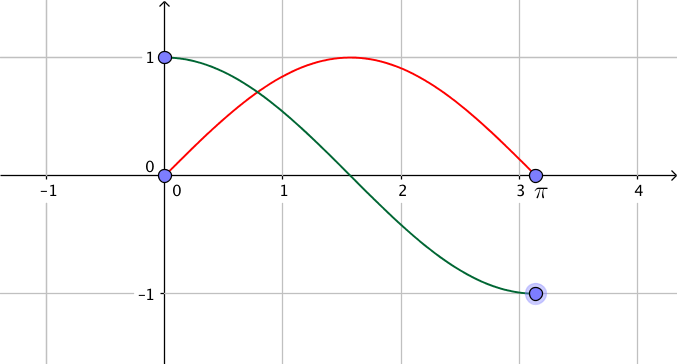
\includegraphics[scale=1,max width=\linewidth,max height=.72\textheight]{surjection.png}$$ байна. 


Графикаас харахад 
$$f(X)=[-1;1]=Y\text{ тул теорем \ref{fun:surj} ёсоор } f(x)=\cos x \text{ сурьектив}$$
$$g(X)=[0;1]\neq Y\Rightarrow g(x)=\sin x \text{ сурьектив биш байна.}$$ 
$x_1 \neq  x_2\in[0;\pi]$ үед $\cos x_1-\cos x_2=-2\sin(\dfrac{x_1-x_2}{2})\sin(\dfrac{x_1+x_2}{2})\neq 0$ тул $f(x)=\cos x$ иньектив байна. 


 $x=\dfrac{\pi}{3} , x=\dfrac{2\pi}{3}$ байхад $g(\dfrac{\pi}{3})=g(\dfrac{2\pi}{3})$ учир $g(x)=\sin x$ иньектив биш байна. 
 
Иймд $f(x)=\cos x$ функц $[0:\pi]$ олонлог дээр биектив ба түүний урвууг $f^{-1}=\arccos x$ гэдэг. Энд $f^{-1}$ функцийн тодорхойлогдох муж $f(X)=Y$ утгийн муж $X$ байна.  

$y=\arccos x$ функцын графикийг дүрслэв. 
$$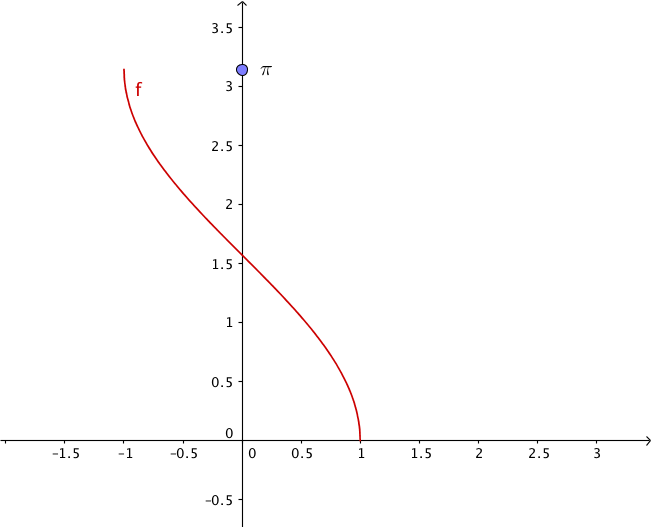
\includegraphics[scale=1.4,max width=\linewidth,max height=.72\textheight]{arccos} $$ 
Хэрэв $f:X \to Y$ биектив функц бол $(x,y)\in\Gamma(f)\Longleftrightarrow (y,x)\in\Gamma(f^{-1})$ байх тул $\Gamma(f)$ ба $\Gamma(f^{-1})$ графикууд  $y=x$ шулууны хувьд тэгш хэмтэй байна. Жишээ болгон $f(x)=\cos x$ ба $y=\arccos x$ функцүүдийн гарфикийг харуулав.
$$
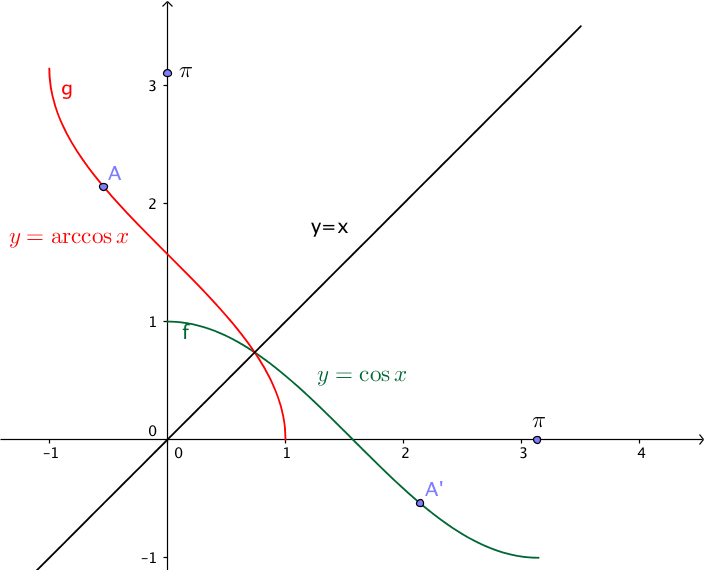
\includegraphics[scale=1.4,max width=\linewidth,max height=.72\textheight]{inverse}$$
\end{example}
\end{frame}

\begin{frame}[allowframebreaks]{Функц}
\begin{definition}
$f:X\to Y$ , $g:Y\to Z$ байг. $$x\to g(f(x))$$ дүрмээр тодорхойлогдох $$g\circ f:X\to Z$$ буулгалтыг $f$ ба $g$ буулгалтуудын үржвэр (композици) гэнэ. 
\end{definition}
\end{frame}

\begin{frame}[allowframebreaks]{Функц}
\begin{example}
$f:\mathbb{R}\to\mathbb{R}$ ба $g:\mathbb{R}\to[0,+\infty)$ функцуудыг
\[
f(x)=2x+1,\qquad g(x)=x^2
\]
гэж тодорхойлъё. Тэгвэл
\begin{itemize}
    \item $(g\circ f)(x)=g(f(x))=g(2x+1)=(2x+1)^2=4x^2+4x+1$
    \item $(f\circ g)(x)=f(g(x))=f(x^2)=2x^2+1$
\end{itemize} байна. 

Дээрх жишээнээс харахад $(g\circ f)(x)\neq (f\circ g)(x)$ байна. Тухайлбал $x=1$ үед 
\[
(g\circ f)(1)=(2\cdot 1+1)^2=9,\qquad (f\circ g)(1)=2\cdot 1^2+1=3.
\]
Иймд ерөнхийдөө $g\circ f\neq f\circ g$, өөрөөр хэлбэл \itcol{композици нь коммутатив биш} байна.
\end{example}
\end{frame}

\begin{frame}[allowframebreaks]{Функц}
\begin{theorem}\label{fun:inv_comp}
$f:X\to Y$ буулгалт биектив бол
 $\forall x\in X$ хувьд $$(f^{-1}\circ f)(x)=x$$ ба $\forall y\in Y$ хувьд $$(f\circ f^{-1})(y)=y$$ 
 байна.
\end{theorem}

\begin{prof}
$f$ биектив тул тодорхойлолт~\ref{fun:inv}-с $\forall y\in Y$ хувьд
$x=f^{-1}(y)$ байх $\exists x\in X$ ба
\[
f\!\left(f^{-1}(y)\right)=f(x)=y
\]
байна. 

Нөгөө талаас $\forall x\in X$ хувьд $f(x)=y\in Y$ гэвэл $f^{-1}(y)=x$ учраас
\[
(f^{-1}\circ f)(x)=f^{-1}(f(x))=f^{-1}(y)=x
\]
\end{prof}
\end{frame}

\begin{frame}[allowframebreaks]{Функц}
\begin{example}
$f:\mathbb{R}\to(0,+\infty)$ ба $g:(0,+\infty)\to\mathbb{R}$ функцуудыг
\[
f(x)=e^x,\qquad g(x)=\ln x
\]
гэж тодорхойлъё. Тэгвэл
\begin{itemize}
    \item $(g\circ f)(x)=g(f(x))=g(e^x)=\ln(e^x)=x$,
    \item $(f\circ g)(x)=f(g(x))=f(\ln x)=e^{\ln x}=x$
    \end{itemize} байна. 
Тодорхойлолт~\ref{fun:inv}-с харахад $g=f^{-1}$ ба $f=g^{-1}$,өөрөөр хэлбэл $\ln x$ ба $e^x$ функцууд бие биенийхээ урвуу функц болно.
\end{example}
\end{frame}

\section{Олонлогийн чадал}
\begin{frame}[allowframebreaks]{Олонлогийн чадал}
\begin{definition}[Олонлогийн чадал (кардиналь)]
$A,B$ олонлогуудийн хувьд $f:A\to B$ \itcol{биектив} буулгалт оршивол тэдгээрийг тэнцүү чадалтай олонлогууд гэнэ. Энэ үед $|A|=|B|$ гэж бичнэ. 


Хэрэв 
\begin{enumerate}
    \item $A$ олонлог $\{1, 2, 3, \ldots n\}$ олонлогтой ижил чадалтай бол түүнийг төгсгөлөг олонлог гээд $|A|=n$
    \item $A$ олонлог $\N$ олонлогтой ижил чадалтай бол түүнийг тоологдом олонлог гээд $|A|=\aleph_0$
    \item $A$ олонлог $\R$ олонлогтой ижил чадалтай бол түүнийг контиунум олонлог гээд $|A|=\mathfrak{c}$
\end{enumerate} гэнэ. $|A|$ нь $A$- дахь элементүүдийн тоог илэрхийлнэ.
\end{definition}
\end{frame}

\begin{frame}[allowframebreaks]{Олонлогийн чадал}
\begin{definition}[Олонлогийн чадалын харьцуулалт]
Хэрэв $f:A\to B$ байх \itcol{иньектив} буулгалт $f$ оршин байвал $B$ олонлогийг $A$ олонлогоос цөөнгүй элемэнттэй гээд $|A|\le |B|$ гэж бичнэ.

Хэрэв $|A|\le |B|$ ба $|A|\ne |B|$ бол  $|A|<|B|$ гэнэ.
\end{definition}
\end{frame}

\begin{frame}[allowframebreaks]{Олонлогийн чадал}
\begin{example}
 $|\emptyset|=0$, \quad $|\{a,b,c\}|=3$.
\end{example}
\end{frame}

\begin{frame}[allowframebreaks]{Олонлогийн чадал}
\begin{example}
$|\mathbb{N}|=|\mathbb{Z}|$ байна. Өөрөөр хэлбэл $$|\{1, 2, 3, \ldots \}|=|\{0, 1, -1, 2, -2, \ldots\}|$$ байна.
 
Үүнийг батлахын тулд $f:\mathbb{N}\to\mathbb{Z}$
биектив буулгалт олоход хангалттай. 
\[
f:\mathbb{N}\to\mathbb{Z},\qquad
f(n)=
\begin{cases}
\dfrac{n}{2}, & n \text{ тэгш,}\\[8pt]
-\dfrac{n-1}{2}, & n \text{ сондгой.}
\end{cases}
\] гэе. 


Функцийн утгуудыг хүснэгтээр харуулбал 
\[
\begin{array}{c|ccccccccc}
n    & 1 & 2 & 3  & 4 & 5  & 6 & 7  & 8 & \cdots \\\hline
f(n) & 0 & 1 & -1 & 2 & -2 & 3 & -3 & 4 & \cdots
\end{array}
\]
болно. 

$f(m)=f(n)$ гэж үзье. Хэрэв 
\begin{itemize}
  \item $m,n$ хоёул тэгш бол
  $\dfrac{m}{2}=\dfrac{n}{2}$, тиймээс $m=n$.

  \item $m,n$ хоёул сондгой бол
  $-\dfrac{m-1}{2}=-\dfrac{n-1}{2}$, тиймээс $m=n$.

  \item $m$ тэгш, $n$ сондгой (эсвэл эсрэгээр) бол
  $f(m)=\dfrac{m}{2}\geq 1>0$ ба $f(n)=-\dfrac{n-1}{2}\leq 0$
  тул $f(m)=f(n)$ байх боломжгүй.
\end{itemize}
Бүх тохиолдолд $f(m)=f(n)\Rightarrow m=n$ тул $f$ иньектив байна.


Дурын $k\in\mathbb{Z}$-г авъя.
\begin{itemize}
  \item $k>0$ бол $n=2k$ тэгш тооны хувьд $f(n)=f(2k)=k$,
  \item $k=0$ бол $n=1$ үед $f(1)=0=k$,
  \item $k<0$ бол $n=1-2k$ сондгой тооны хувьд   
  \[
  f(1-2k)=-\frac{(1-2k)-1}{2}=\frac{2k}{2}=k
  \]
\end{itemize} байна.
Бүх $k\in\mathbb{Z}$-д $f(n)=k$ байх $n\in\mathbb{N}$ олдох тул $f$ сурьектив байна.


$f$ иньектив ба сурьектив тул биектив байна. Тиймээс $$|\mathbb{N}|=|\mathbb{Z}|$$ байна.
\end{example}
\end{frame}

\begin{frame}[allowframebreaks]{Олонлогийн чадал}
\begin{example}
    \begin{enumerate}
        \item $|(0,1)|=|\mathbb{R}|=\mathfrak{c}$ \,(континуум, тоологдошгүй).
  \item Дурын $A$ олонлогийн хувьд $|\mathcal{P}(A)|=2^{|A|}>|A|$ байна.
\end{enumerate}
\end{example}
\end{frame}

% Семинар ба гэрийн даалгавар
% Лекц 2: семинар ба гэрийн даалгавар. Бодлогууд хөнгөнөөс хүнд рүү эрэмбэлэгдсэн.

\ProblemSet{Семинар 2}
\begin{frame}[allowframebreaks]{Семинар 2}
\pgroup{Олонлог.}
\begin{plist}
\pr{Логик хэлбэрээр бич: $x\in A\cup B$, $x\in A\cap B$, $x\in A\setminus B$.}
\pr{$|A|=5$, $|B|=7$, $A\cap B=\emptyset$ бол $|A\cup B|$ хэд вэ?}
\pr{$U=\mathbb Z$, $A$ нь тэгш тоонууд, $B$ нь 3-т хуваагддаг тоонууд. $A^c$, $B^c$, $A\triangle B$-г тодорхойл. Энд $A\triangle B:=(A\setminus B)\cup(B\setminus A)$.}
\pr{Батал: а) $A\subseteq B\Leftrightarrow A\cap B=A$; б) $A\subseteq B\Leftrightarrow A\cup B=B$.}
\pr{$A\subseteq B\subseteq C$ бол $C\setminus B\subseteq C\setminus A$ болохыг батал.}
\pr{$A\times(B\cup C)=(A\times B)\cup(A\times C)$ болохыг батал.}
\pr{$A\times B=B\times A$ байх нөхцөлийг ол.}
\pr{Төгсгөлөг олонлогуудын хувьд $|A\cup B|=|A|+|B|-|A\cap B|$ болохыг батал.}
\end{plist}
\pgroup{Функц.}
\begin{plist}
\pr{$X=\{a,b\}$, $Y=\{1,2,3\}$. $X\to Y$ бүх буулгалтын тоог ол.}
\pr{$f(x)=x^2+1$, $g(x)=3x-1$, $h(x)=\frac{x+1}{3}$ бол $f\circ g$, $g\circ g$, $g\circ f$, $g\circ h$, $(f\circ g)\circ h$, $f\circ(g\circ h)$-г ол.}
\pr{Тодорхойлогдох мужийг ол: а) $y=\sqrt{x^3-3x+2}$; б) $y=\arcsin(2x-1)$; в) $y=\dfrac{x^3-3x}{x^2-1}$; г) $y=\ln(3-x-2x^2)$.}
\pr{Графикийг зур: а) $y=2x-3$; б) $y=-x^2-2x+3$; в) $y=x^3-3x$; г) $y=\dfrac{\sin x}{x}$; д) $y=\ln x$.}
\pr{$h(x)=\dfrac{x}{1+x^2}$ тэгш, сондгой эсэхийг тодорхойл.}
\pr{$g(x)=\dfrac{f(x)+f(-x)}{2}$ тэгш функц болохыг батал.}
\pr{$f:\R\to\R$, $f(x)=x^2+1$. Иньектив, сурьектив, биектив эсэхийг тогтоо. Дүрийг ол.}
\pr{$f:\R\to\R$, $f(x)=x^3-3x$. Иньектив, сурьектив, биектив эсэхийг тогтоо. Урвуутай бол урвууг ол.}
\pr{$f:[0,\pi]\to[-1,1]$, $f(x)=\cos x$. Урвууг нь бич.}
\pr{$g:[-\frac\pi2,\frac\pi2]\to[-1,1]$, $g(x)=\sin x$. Урвууг нь бич.}
\pr{$f:[-1,1]\to[0,2]$ байх а) иньектив ч биш, сурьектив ч биш; б) иньектив биш, сурьектив; в) биектив буулгалтын жишээг графикаар үзүүл.}
\pr{$f:X\to Y$, $g:Y\to Z$ иньектив бол $g\circ f$ иньектив болохыг батал.}
\end{plist}
\end{frame}

\ProblemSet{Гэрийн даалгавар 2}
\begin{frame}[allowframebreaks]{Гэрийн даалгавар 2}
\pgroup{Олонлог.}
\begin{plist}
\pr{$|A|=5$, $|B|=4$, $|A\cap B|=2$ бол $|A\cup B|$ хэд вэ?}
\pr{$A\subseteq U$ бол $A\cup A^c=U$, $A\cap A^c=\emptyset$ болохыг батал.}
\pr{$A=\{1,2,3,4\}$, $B=\{3,4,5\}$ бол $A\cup B$, $A\cap B$, $A\setminus B$, $B\setminus A$-г ол. $A\times B$ хэдэн элементтэй вэ?}
\pr{$\{a,b,c\}$ олонлогийн бүх дэд олонлогийг жагсаа. $n$ элементтэй олонлог хэдэн дэд олонлогтой вэ?}
\pr{$X=\{0,1\}^3$. $|X|$-ийг олж, элементүүдийг жагсаа.}
\pr{Батал: $(A\cup B)\setminus C=(A\setminus C)\cup(B\setminus C)$.}
\pr{Батал: $(A\cap B)^c=A^c\cup B^c$.}
\pr{Батал: $A\triangle B=(A\cup B)\setminus(A\cap B)$.}
\pr{Батал: $A\setminus(B\cup C)=(A\setminus B)\cap(A\setminus C)$.}
\end{plist}
\pgroup{Функц, тэгш ба сондгой функц.}
\begin{plist}
\pr{$f:\R\to\R$, $f(x)=ax+b$. Иньектив, сурьектив байх $a,b$-ийн нөхцөлийг ол.}
\pr{$f:\R\to\R$, $f(x)=x^2$ яагаад урвуугүй вэ? Ямар мужид хязгаарлавал урвуутай болох вэ?}
\pr{$f:\R\setminus\{3\}\to\R\setminus\{2\}$, $f(x)=\dfrac{2x+1}{x-3}$ биектив болохыг харуулж, урвууг ол.}
\pr{$h(x)=x^4-3x^2+2$ тэгш, сондгой эсэхийг дүгнэ.}
\pr{$p(x)=x^5-2x^3+x$ тэгш, сондгой эсэхийг дүгнэ.}
\pr{$f,g$ тэгш бол $f\cdot g$ тэгш болохыг батал.}
\pr{$f,g$ сондгой бол $f\cdot g$ тэгш болохыг батал.}
\pr{$f$ тэгш, $g$ сондгой бол $f\circ g$ ямар функц болохыг шалга.}
\pr{$g(x)=\dfrac{f(x)-f(-x)}{2}$ сондгой функц болохыг батал.}
\pr{Тэгш хэмтэй мужид тодорхойлогдсон дурын функцийг тэгш ба сондгой функцийн нийлбэрээр нэг утгатай илэрхийлж болохыг батал.}
\end{plist}
\pgroup{Дараалал.}
\begin{plist}
\pr{$d_n=n^2$ дараалал өсөх, үл буурах, буурах алин бэ?}
\pr{$e_n=(-1)^n$ монотон уу? Зааглагдсан уу?}
\pr{$a_n=\dfrac{n}{n+1}$ монотон уу? Дээд, доод зааг нь юу вэ?}
\pr{$a_1=2$, $a_{n+1}=2a_n+1$ бол ерөнхий гишүүнийг ол.}
\pr{$b_1=1$, $b_{n+1}=3b_n-2$ бол $b_n$-ийг ол.}
\end{plist}
\pgroup{Буулгалт ба олонлогийн чадал.}
\begin{plist}
\pr{$f:X\to Y$, $g:Y\to Z$ сурьектив бол $g\circ f$ сурьектив болохыг батал.}
\pr{$g\circ f$ иньектив бол $f$ иньектив болохыг батал. $g$ иньектив байх албатай юу?}
\pr{$f:X\to Y$, $A,B\subseteq X$ бол $f(A\cup B)=f(A)\cup f(B)$, $f(A\cap B)\subseteq f(A)\cap f(B)$ болохыг батал. Тэнцэл биелэхгүй жишээ гарга.}
\pr{$\N$ ба тэгш натурал тоонуудын олонлог, мөн $\N$ ба $\mathbb Z$ тэнцүү чадалтай болохыг харуул.}
\pr{$A=\{x\in\R\mid x^3+2x^2-x-2>0\}$, $B=\{x\in\R\mid x^2+ax+b\le0\}$. $A\cup B=\{x\mid x+2>0\}$, $A\cap B=\{x\mid 1<x\le3\}$ байх $a,b$-ийн бүх утгыг ол.}
\pr{$A\subset\N$ олонлог а) $1\in A$; б) $2n+1\in A\Rightarrow n\in A$; в) $n\in A\Rightarrow 3n+1\in A$ нөхцлүүдийг хангадаг бол $2,17,2025,1000000\in A$ байх уу?}
\end{plist}
\end{frame}

% Лекц 3. Тоон олонлогууд
% Эх: latex/lectures/lec03-numbers.tex (scripts/latex_to_beamer.py-ээр хөрвүүлсэн)
% Frame бүр слайдад нэг (эсвэл allowframebreaks-аар хэд хэдэн) хуудас болно;
% хэвлэх хувилбарт frame-ийн хил харагдахгүй, текст үргэлжилсэн байна.

\MathLecture{3}{Тоон олонлогууд}

\section{Натурал тоо}
\begin{frame}[allowframebreaks]{Натурал тоо}
Энд бид натурал тооны онолыг Пеаногийн (Dedekind–Peano) аксиомоор байгуулна. 
\end{frame}

\section*{Жузеппе Пеано (1858–1932)}
\begin{frame}[allowframebreaks]{Жузеппе Пеано (1858–1932)}
\noindent
\begin{minipage}[t]{0.2\textwidth}
  \vspace{0pt}
  \centering
  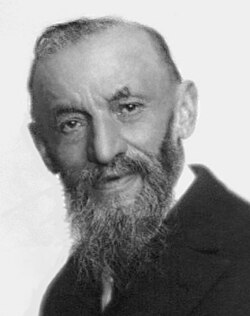
\includegraphics[width=\linewidth,max width=\linewidth,max height=.72\textheight]{Peano.jpg}
\end{minipage}\hfill
\begin{minipage}[t]{0.78\textwidth}
  \vspace{0pt}
  \textbf{Жузеппе Пеано} нь Италийн математикч, логикийн суурь судлаач.
  1889 онд натурал тоог аксиомчилсон (\emph{Dedekind–Peano} аксиомууд) бүтээлээ
  хэвлүүлж, 1890 онд дифференциал тэгшитгэлийн судалгааны үр дүнд \emph{Пеаногийн муруй}-г танилцуулсан.
  Орчин үеийн тэмдэглэгээнд ихээхэн нөлөөлсөн (жиш., $\in$ тэмдгийн эх сурвалж
  нь Пеаногийн $\varepsilon$). Ихэвчлэн Турины их сургуульд ажиллаж,
  \emph{Formulario Mathematico} цувралыг эмхэтгэсэн. \vspace{1cm}
  
\end{minipage}
\end{frame}

\begin{frame}[allowframebreaks]{Жузеппе Пеано (1858–1932)}
\begin{definition}[Натурал тоон олонлог]\label{натурал тоо}
    Хэрэв $\N$ олонлог ба түүний  $\mathbb{a}$ элемент, $$S:\N\to\N$$ буулгалт өгөгдсөн ба $(\N, \mathbb{a}, S)$ гуравт дараах 5 аксиомыг хангадаг бол $\N$ олонлогийг натурал тоон олонлог гэнэ. 
\begin{enumerate}[label=\textbf{A\arabic*})]
  \item $\mathbb{a}\in\N$.
  \item $n\in \N$ бол $S(n)\in \N$ байна. \hfill ($S(n)$-г $n$-н залгамжлагч гэе)
  \item $\forall n\in\N$ бол $S(n)\ne \mathbb{a}$ байна. \hfill ($\mathbb{a}$ нь залгамжлагч биш)
  \item $ m\neq n\in\N$ бол $S(m)\neq S(n)$ байна. \hfill (\emph{иньектив})
  \item Хэрэв $P(n)$ нь $n$ гэсэн натурал тооноос хамаарсан хэллэг бөгөөд
\begin{itemize}
    \item $n=1$ үед $P(1)$ үнэн
    \item ямар нэг $n\in \mathbb{N}$ хувьд $P(n)$ үнэн байвал заавал $P(S(n))$ үнэн
\end{itemize} нөхцлүүдийг хангадаг бол $P(n)$ хэллэг $\forall n\in\mathbb{N}$ хувьд үнэн байна.
\end{enumerate}
\end{definition}
\end{frame}

\begin{frame}[allowframebreaks]{Жузеппе Пеано (1858–1932)}
\begin{example}[Математик индукц]
  Цаашид $\mathbb{a}$-г 1, $S(\mathbb{a})$-г 2, $S(S(\mathbb{a}))$-г 3 гэх мэт тэмдэглэвэл $$\{\mathbb{a}, S(\mathbb{a}), S(S(\mathbb{a})), \ldots \}=\{1, 2, 3, \ldots \}\subset \N$$ болно.  Одоо $\{1, 2, 3, \ldots \}=\N$ болохыг батлая. 

  $b\in\N$ бол $P(b):\{b=1\land b=S(n)\text{\, байх\, } n\in\N \text{\, олдоно.}\}$ гэсэн хэллэг авч үзье. Энэ хэллэг бүх $b$ натуралын хувьд үнэн байхыг батлая. $\textbf{A5)}$ аксиомыг хэрэглэе.
  \begin{enumerate}
      \item Хэрэв $b=1$ бол $P(1)$ үнэн
    \item ямар нэг $1\neq b\in \mathbb{N}$ хувьд $P(b)$ үнэн байвал $b=S(n)$ гэсэн үг. Иймд заавал $S(b)=S(S(n))$ болох тул $S(b)$ хувьд $S(S(n))$ олдож байна. Иймд $P(S(b))$ үнэн байна. 
  \end{enumerate}
   Иймд $\textbf{A5)}$ аксиомоор $P(b):\{b=1\land b=S(n)\text{\, байх\, } n\in\N \text{\, олдоно.}\}$ гэсэн хэллэг $\forall b\in\mathbb{N}$ хувьд үнэн байна. 
\end{example}
\end{frame}

\begin{frame}[allowframebreaks]{Жузеппе Пеано (1858–1932)}
\begin{theorem}
   $n\in\N , n\neq 1$ бол $n=S(m)$ байх $m$ ганц олдоно. $m=\underbrace{S(S\ldots S(}_{n-1}1)\ldots)$ байна.
\end{theorem}
\begin{prof}
     Семинарын бодлого хар.
\end{prof}
\end{frame}

\begin{frame}[allowframebreaks]{Жузеппе Пеано (1858–1932)}
\begin{theorem}[(Математик индукц)]\label{mathind}
$n\in\N$ ба $P(n)$ шинж өгөгдөхөд 
\begin{enumerate}
    \item $P(1)$ үнэн
    \item $\forall n\,(P(n)$ хувьд $P(1), P(2), \ldots P(n)$ үнэн бол $P(S(n)))$ үнэн байдаг
\end{enumerate} чанартай байвал $\forall n\in\N$ хувьд $P(n)$ шинж үнэн байна.
\end{theorem}
\begin{prof}
    $\mathbb{A5}$ аас мөрдөнө.
\end{prof}
\end{frame}

\section{Натурал тооны нэмэх, үржих үйлдэл ба зэрэгт дэвшүүлэх}
\subsection{Нэмэх}
\begin{frame}[allowframebreaks]{Нэмэх}
\begin{definition}[Hэмэх үйлдэл] $+: \N\times \N\to\N$ буулгалт (үйлдэл)-г дараах дүрмээр байгуулая. $\forall n , m\in\N$ хувьд $+(n,m)=n+m$ гэж тэмдэглэе.
\begin{enumerate}[label=\textbf{N\arabic*})]
    \item $ n+1= S(n)$
    \item $n+S(m)=S(n+m)$
\end{enumerate} 
\end{definition}
\end{frame}

\begin{frame}[allowframebreaks]{Нэмэх}
\begin{example}
    \begin{enumerate}
        \item $1+1=S(1)=2$
        \item $2+1=S(2)=3$
        \item $5+2=5+S(1)=S(5+1)=S(6)=7$
        \item $5+3=5+S(2)=S(5+2)=S(7)=8$
    \end{enumerate}
\end{example}
\end{frame}

\begin{frame}[allowframebreaks]{Нэмэх}
\begin{theorem}\label{nemeh 1}
$\forall n$ хувьд $1+n=n+1$ байна.
\end{theorem}
\begin{proof}
Теорем \ref{mathind} ашиглан индукц хийе. 
\begin{enumerate}
    \item $n=1$: $1+1=1+1$ 
    \item Xэрэв $n\neq 1 $ гэж үзвэл $1+1=1+1 \, , 1+2=2+1 \, , 1+3=3+1 \, , \ldots ,  1+n=n+1 $ гэе. 
    
    Одоо $S(n)+1=1+S(n)$ батлая. $1+S(n)=S(1+n)$ (нэмэхийн 2-р аксиом). 
    
    Нөгөө талаас $S(n)+1=S(S(n))=S(n+1)$ (нэмэхийн 1-р аксиом) болох ба бид $ 1+n=n+1 $ гэж үзсэн тул  $$1+S(n)=S(1+n)=S(n+1)=S(S(n))=S(n)+1$$ тул 
    $S(n)+1=1+S(n)$ батлагдав.
    \qedhere
\end{enumerate}  
\end{proof}
\end{frame}

\begin{frame}[allowframebreaks]{Нэмэх}
\begin{theorem}[Нэмэхийн коммутатив чанар]
$\forall m,n\in\N$ бол $ m+n=n+m$ байна.
\end{theorem}
\begin{prof}
$\varphi_n(m):\, m+n=n+m$ хэллэгийг $n$-ээр индукцлэн батлая. 

$n=1$: $1+m=m+1$ байхыг Теорем \ref{nemeh 1} баталсан. 

Индукцийн алхам: $\varphi_n\Rightarrow\varphi_{S(n)}$.
\begin{align*}
 m+S(n)&=S(m+n)\quad(\textbf{N2})\\
           &=S(n+m)\quad(\text{индукцийн таамаглал})\\
           &=n+S(m)\quad(\textbf{N2 }\text{ урвуугаар ашиглав}).
\end{align*}
\end{prof}
\end{frame}

\begin{frame}[allowframebreaks]{Нэмэх}
\begin{theorem}[Нэмэхийн ассоциатив чанар]
$\forall \ell,m,n:\ (\ell+m)+n=\ell+(m+n)$.
\end{theorem}
\begin{prof}
$n$-ээр индукцлэе. 

Суурь: $(\ell+m)+1=S(\ell+m)=\ell+S(m)=\ell+(m+1).$ 

Индукцийн алхам:
\[(\ell+m)+S(n)=S\big((\ell+m)+n\big)=S\big(\ell+(m+n)\big)=\ell+S(m+n)=\ell+(m+S(n)).\]
\end{prof}
\end{frame}

\subsection{Үржих}
\begin{frame}[allowframebreaks]{Үржих}
 \begin{definition}[Үржих үйлдэл] $ \times : \N\times \N\to\N$ буулгалт (үйлдэл)-г дараах дүрмээр байгуулая. $\forall n , m\in\N$ хувьд $\times(n,m)=n\cdot m$ гэж тэмдэглэе.
\begin{enumerate}[label=\textbf{U\arabic*})]
    \item $ n\cdot 1= n$
    \item $n\cdot S(m)=n\cdot m+n$
\end{enumerate} 
\end{definition}
\end{frame}

\begin{frame}[allowframebreaks]{Үржих}
\begin{example}
    \begin{enumerate}
    \item $1\cdot 1=1$
    \item $2\cdot 1=2$
    \item $5\cdot 2=5\cdot S(1)=5\cdot 1+5=5+5=10$
    \item $5\cdot 3=5\cdot S(2)=5\cdot 2+5=10+5=15$
    \end{enumerate}
\end{example}
\end{frame}

\begin{frame}[allowframebreaks]{Үржих}
\begin{theorem}[Дистрибутив]\label{distributive}
$\forall a,b,c\in\N$ бол $a\cdot(b+c)=a\cdot b+a\cdot c$ байна.
\end{theorem}
\begin{prof}
$c$-ээр индукцлэе. 

Суурь: $a\cdot(b+1)=a\cdot S(b)=a\cdot b+a=a\cdot b+a\cdot 1$. 

Индукцийн алхам:
\begin{align*}
a\cdot S(c)&=a\cdot c+a,\\
a\cdot(b+S(c))&=a\cdot S(b+c)=a\cdot(b+c)+a=\big(a\cdot b+a\cdot c\big)+a= a\cdot b+a\cdot S(c).
\end{align*}
\end{prof}
\end{frame}

\begin{frame}[allowframebreaks]{Үржих}
\begin{theorem}\label{urjih 1}
$\forall n\in\N$ бол $1\cdot n=n\cdot 1$ байна.
\end{theorem}
\begin{prof}
     Семинарын бодлого хар.
\end{prof}
\end{frame}

\begin{frame}[allowframebreaks]{Үржих}
\begin{theorem}[Үржихийн коммутатив]
$\forall m,n\in\N$ бол $ m\cdot n=n\cdot m$ байна.
\end{theorem}
\begin{prof}
$n$-ээр индукцлэе. 

Суурь: $n=1$: $m\cdot 1=m=1\cdot m$ байхыг Теорем \ref{urjih 1} батласан. 
Алхам:
\[m\cdot S(n)=m\cdot n+m= n\cdot m+m=S(n)\cdot m.\]
\end{prof}
\end{frame}

\begin{frame}[allowframebreaks]{Үржих}
\begin{theorem}[Үржихийн ассоциатив]
$\forall a,b,c:\ (a\cdot b)\cdot c=a\cdot(b\cdot c)$.
\end{theorem}
\begin{prof}
     Семинарын бодлого хар.
\end{prof}
\end{frame}

\subsection{Зэрэг}
\begin{frame}[allowframebreaks]{Зэрэг}
 \begin{definition}[Зэрэг] $ A: \N\times \N\to\N$ буулгалт (үйлдэл)-г дараах дүрмээр байгуулая. $\forall n , m\in\N$ хувьд $A(n,m)=n^ m$ гэж тэмдэглэе.
\begin{enumerate}[label=\textbf{Z\arabic*})]
    \item $ n^1= n$
    \item $n^{S(m)}=n^ m\cdot n$
\end{enumerate} 
\end{definition}
\[n^{1}=n,\qquad n^{S(m)}=n^{m}\cdot n.\]
Индукцээр $n^{a+b}=n^a\cdot n^b$, $n^{a\cdot b}=(n^a)^b$ зэрэг үндсэн томьёонууд батлагдана.
\end{frame}

\subsection{Эрэмбэ тодорхойлох}
\begin{frame}[allowframebreaks]{Эрэмбэ тодорхойлох}
\begin{definition}
$\forall m,n\in\N$ үед $n=m+k$ байх $\exists k\in\N$ олддог $n>m$ гэнэ. Цаашид $n=m$ эсвэл $n>m$ бол $n\ge m$ гэж тэмдэглэе.
\end{definition}
\end{frame}

\begin{frame}[allowframebreaks]{Эрэмбэ тодорхойлох}
\begin{theorem}[Эрэмбийн үндсэн чанарууд]
Дараах нь биелнэ.
\begin{enumerate}\label{erembe}
  \item (Рефлексив) $n\le n$.
  \item (Транзитив) $\big(m\le n\ \,\wedge\,\ n\le p\big)\Rightarrow m\le p$.
  \item (Анти-симметр) $m\le n$ ба $n\le m$ бол $m=n$.
\end{enumerate}
\end{theorem}
\begin{prof}
(i) $n=n$ тул $n\le n$. 

(ii) $m+k=n$, $n+\ell=p$ бол $m+(k+\ell)=p$ тул $m\le p$. 

(iii) Хэрэв $n\neq m$ бол $m+k=n$, $n+\ell=m$-ээс $m+(k+\ell)=m$ тул $S(m-1)+(k+\ell)=S(m-1)$ болно. Иймд $(m-1)+(k+\ell)=(m-1)$ болно. Үүнтэй ижлээр давтвал $1+(k+\ell)=1$ болох ба эндээс $S(k+\ell)=1$ болж зөрчил гарна. Иймд $n=m$.
\end{prof}
\end{frame}

\begin{frame}[allowframebreaks]{Эрэмбэ тодорхойлох}
\begin{theorem}[Трихотом]
Ямар ч $m,n$-ын хувьд яг нэг нь үнэн: $m<n$, $m=n$ эсвэл $m>n$.
\end{theorem}
\end{frame}

% Семинар ба гэрийн даалгавар
% Лекц 3: семинар ба гэрийн даалгавар. Бодлогууд хөнгөнөөс хүнд рүү эрэмбэлэгдсэн.
% Натурал тоо 1-ээс эхэлнэ (лекцийн A1--A5, N1--N2, U1--U2, Z1--Z2).

\ProblemSet{Семинар 3}
\begin{frame}[allowframebreaks]{Семинар 3}
\pgroup{Сануулга.}
$n+1=S(n)$, $n+S(m)=S(n+m)$; $n\cdot1=n$, $n\cdot S(m)=n\cdot m+n$; $n^1=n$, $n^{S(m)}=n^m\cdot n$;
$m<n\iff\exists k\ (n=m+k)$. Нэмэх, үржихийн коммутатив, ассоциатив, дистрибутив чанарууд ба трихотомийг ашиглаж болно.
$2=S(1)$, $3=S(2)$, \dots{} гэж тэмдэглэнэ.
\pgroup{Аксиом ба тодорхойлолтоос батал.}
\begin{plist}
\pr{$2+2=4$}
\pr{$2+3\ne6$}
\pr{$2\cdot4=8$}
\pr{$n+2=S(S(n))$}
\pr{$n\cdot2=n+n$}
\pr{$n\cdot3=n+n+n$}
\pr{$1^n=1$ (индукцээр)}
\pr{$a^n\ge1$}
\pr{$\forall n\ (n\ne S(n))$}
\pr{$n\ne1$ бол $n>1$}
\pr{$m+n\ne m$}
\pr{$a+c=b+c\Rightarrow a=b$ ($c$ дээр индукцлэн, A4-ийг ашигла)}
\end{plist}
\pgroup{Эрэмбэ ба зэрэг.}
\begin{plist}
\pr{$a<b\Rightarrow S(a)\le b$}
\pr{$a<b\Rightarrow a+c<b+c$}
\pr{$a<b\Leftrightarrow a\cdot c<b\cdot c$}
\pr{$a^{m+n}=a^m\cdot a^n$-г $n$ дээр индукцлэн батал.}
\pr{$a^{mn}=(a^m)^n$-г $n$ дээр индукцлэн батал.}
\pr{$(ab)^n=a^nb^n$}
\pr{$1+2+\cdots+n=\dfrac{n(n+1)}{2}$}
\pr{$n<2^n$}
\end{plist}
\end{frame}

\ProblemSet{Гэрийн даалгавар 3}
\begin{frame}[allowframebreaks]{Гэрийн даалгавар 3}
\pgroup{Аксиом ба тодорхойлолтоос батал.}
\begin{plist}
\pr{$3+4=7$}
\pr{$3\cdot3=9$}
\pr{$2^3=8$}
\pr{$n+3=S(S(S(n)))$}
\pr{$S(a)+b=S(a+b)$-г $b$ дээр индукцлэн батал.}
\pr{$a+S(b)=S(a)+b$}
\pr{$1\cdot n=n$ (индукцээр)}
\pr{$S(n)\cdot m=n\cdot m+m$}
\pr{$(a+b)\cdot c=a\cdot c+b\cdot c$}
\pr{$(a+b)^2=a^2+2ab+b^2$ томьёог зөвхөн коммутатив, ассоциатив, дистрибутив чанараас гарга.}
\pr{$a\cdot b=a\Rightarrow b=1$}
\end{plist}
\pgroup{Эрэмбэ.}
\begin{plist}
\pr{$a\le b\Rightarrow a<b+c$}
\pr{$a\le b$ ба $b<c$ бол $a<c$}
\pr{$a\le b\Rightarrow a\cdot c\le b\cdot c$}
\pr{$a<b$, $c<d$ бол $a+c<b+d$}
\pr{$a<b$, $c<d$ бол $a\cdot c<b\cdot d$}
\pr{$n$ ба $S(n)$-ийн хооронд натурал тоо байхгүй: $n<m<S(n)$ байх $m$ олдохгүй.}
\pr{$a\ne1$ бол $a=S(m)$ байх $m$ цор ганц олдоно.}
\pr{$a>1$ бол $a^n<a^{n+1}$}
\pr{$a\cdot c=b\cdot c\Rightarrow a=b$}
\pr{$a\le b\iff a=b$ эсвэл $\exists k\ (b=a+k)$ тодорхойлолтыг ашиглан трихотомийг бүрэн батал.}
\end{plist}
\pgroup{Математик индукц.}
\begin{plist}
\pr{$1+3+5+\cdots+(2n-1)=n^2$}
\pr{$1^3+2^3+\cdots+n^3=\Bigl(\dfrac{n(n+1)}{2}\Bigr)^2$}
\pr{$1\cdot2+2\cdot3+\cdots+n(n+1)=\dfrac{n(n+1)(n+2)}{3}$}
\pr{$n^3+2n$ нь 3-т хуваагдана.}
\pr{$n\ge4$ үед $n!>2^n$}
\pr{Бернуллийн тэнцэтгэл биш: $x>-1$ бол $(1+x)^n\ge1+nx$.}
\pr{$n\ge8$ бол $n=3a+5b$ байх $a,b\ge0$ бүхэл тоо олдоно.}
\pr{$n\ge2$ натурал тоо бүр анхны тоонуудын үржвэрт задарна (бүрэн индукц).}
\pr{$\N$-ийн хоосон биш дэд олонлог бүр хамгийн бага элементтэй болохыг индукцийн аксиомоос батал.}
\end{plist}
\end{frame}

% Лекц 4. Функцийн ойлголт, олон гишүүнт ба рационал функц
% Эх: latex/lectures/lec04-basic-functions.tex (scripts/latex_to_beamer.py-ээр хөрвүүлсэн)
% Frame бүр слайдад нэг (эсвэл allowframebreaks-аар хэд хэдэн) хуудас болно;
% хэвлэх хувилбарт frame-ийн хил харагдахгүй, текст үргэлжилсэн байна.

\MathLecture{4}{Функцийн ойлголт, олон гишүүнт ба рационал функц}

\providecommand{\R}{\mathbb{R}}
\providecommand{\N}{\mathbb{N}}
\providecommand{\tg}{\operatorname{tg}}
\providecommand{\ctg}{\operatorname{ctg}}
\providecommand{\arctg}{\operatorname{arctg}}
\providecommand{\arcctg}{\operatorname{arcctg}}
\section{Функц ба түүний үндсэн ойлголтууд}
\begin{frame}[allowframebreaks]{Функц ба түүний үндсэн ойлголтууд}
\begin{definition}[Функц]
$X,Y\subset\R$ байг. $X$ олонлогийн $x$ элемент бүрд $Y$ олонлогийн яг нэг
$y=f(x)$ элементийг харгалзуулсан дүрмийг \itcol{функц} гээд $f:X\to Y$ гэж тэмдэглэнэ.
\begin{itemize}
  \item $D(f)=X$ — \itcol{тодорхойлогдох муж},
  \item $E(f)=\{f(x)\mid x\in X\}\subset Y$ — \itcol{утгын муж},
  \item $\Gamma(f)=\{(x,f(x))\mid x\in X\}\subset\R^2$ — $f$-ийн \itcol{график}.
\end{itemize}
\end{definition}
\end{frame}

\begin{frame}[allowframebreaks]{Функц ба түүний үндсэн ойлголтууд}
\begin{remark}
Функцийг зөвхөн томьёогоор өгсөн бол тодорхойлогдох муж нь уг томьёо утгатай байх
бүх $x$-ийн олонлог гэж ойлгоно.
\end{remark}
\end{frame}

\begin{frame}[allowframebreaks]{Функц ба түүний үндсэн ойлголтууд}
\begin{example}
$f(x)=\sqrt{4-x^2}+\dfrac{1}{x}$ функцийн хувьд $4-x^2\ge 0$ ба $x\neq0$ байх ёстой тул
$D(f)=[-2;0)\cup(0;2]$.
\end{example}
\end{frame}

\begin{frame}[allowframebreaks]{Функц ба түүний үндсэн ойлголтууд}
\begin{remark}[Түгээмэл алдаа]
$\sqrt{x^2}=|x|$ бөгөөд $x$-тэй тэнцүү биш: $\sqrt{(-3)^2}=3\neq-3$.
\end{remark}
\end{frame}

\begin{frame}[allowframebreaks]{Функц ба түүний үндсэн ойлголтууд}
\begin{definition}[Инъектив, сюръектив, биектив]
$f:X\to Y$ функц байг.
\begin{itemize}
  \item $x_1\neq x_2 \Rightarrow f(x_1)\neq f(x_2)$ бол $f$-г \itcol{инъектив} гэнэ.
  \item $\forall y\in Y$ хувьд $f(x)=y$ байх $x\in X$ олддог, өөрөөр хэлбэл $E(f)=Y$ бол
        $f$-г \itcol{сюръектив} гэнэ.
  \item Инъектив ба сюръектив бол $f$-г \itcol{биектив} гэнэ.
\end{itemize}
\end{definition}
\end{frame}

\begin{frame}[allowframebreaks]{Функц ба түүний үндсэн ойлголтууд}
\begin{example}
$f(x)=x^2$ байг.
\begin{itemize}
  \item $f:\R\to\R$ нь инъектив биш ($f(-1)=f(1)$), сюръектив ч биш ($x^2=-1$ шийдгүй).
  \item $f:[0;+\infty)\to[0;+\infty)$ нь биектив.
\end{itemize}
Эндээс харахад функцийн чанар нь зөвхөн томьёоноос бус, $X$ ба $Y$ мужаас хамаардаг.
\end{example}
\end{frame}

\section{Функцийг ангилах}
\subsection{Тэгш ба сондгой функц}
\begin{frame}[allowframebreaks]{Тэгш ба сондгой функц}
\begin{definition}[Тэгш ба сондгой функц]
$x\in X \Rightarrow -x\in X$ бол $X\subset\R$ олонлогийг \itcol{тэгш хэмтэй} гэнэ.
Тэгш хэмтэй $X$ дээр тодорхойлогдсон $f:X\to\R$ функцийг
\begin{itemize}
  \item $\forall x\in X$ үед $f(-x)=f(x)$ бол \itcol{тэгш функц},
  \item $\forall x\in X$ үед $f(-x)=-f(x)$ бол \itcol{сондгой функц},
  \item дээрх хоёрын алийг нь ч хангахгүй бол \itcol{тэгш ч биш, сондгой ч биш функц} гэнэ.
\end{itemize}
\end{definition}
\end{frame}

\begin{frame}[allowframebreaks]{Тэгш ба сондгой функц}
\begin{remark}[Мужийн шаардлага]
Тэгш/сондгой эсэхийг ярихдаа $X$ заавал тэгш хэмтэй байх ёстой. Жишээ нь
$X=[0;1]$ бол $x=1$ үед $f(-1)$ тодорхойлогдохгүй тул энэ ангилал хамаарахгүй.
\end{remark}
\end{frame}

\begin{frame}[allowframebreaks]{Тэгш ба сондгой функц}
\begin{remark}[Графикийн тайлбар]
$f$ тэгш бол
\[
  (x,\,f(x))\in\Gamma(f) \;\Longleftrightarrow\; (-x,\,f(x))\in\Gamma(f).
\]
$(x,y)$ цэгийг $OY$ тэнхлэгийн хувьд тэгш хэмтэй хувиргавал $(-x,y)$ цэг гарна.
Иймд тэгш функцийн график $OY$ тэнхлэгийн хувьд тэгш хэмтэй.

$f$ сондгой бол
\[
  (x,\,f(x))\in\Gamma(f) \;\Longleftrightarrow\; (-x,\,-f(x))\in\Gamma(f).
\]
$(x,y)$ цэгийг координатын эхийн хувьд тэгш хэмтэй хувиргавал $(-x,-y)$ цэг гарна.
Иймд сондгой функцийн график $O(0,0)$ цэгийн хувьд тэгш хэмтэй.
\end{remark}
\end{frame}

\begin{frame}[allowframebreaks]{Тэгш ба сондгой функц}
\begin{example}[Тэгш ба сондгой функцийн график]
$f(x)=x^2-2$ ба $g(x)=x^3-3x$ функцүүдийн графикийг нэг тэнхлэг дээр дүрслэв.
\begin{itemize}
  \item $f(-x)=f(x)$ тул $(-a,f(a))$ ба $(a,f(a))$ цэгүүд $OY$ тэнхлэгийн хоёр талд
        ижил өндөрт оршино (улаан парабол).
  \item $g(-x)=-g(x)$ тул $(-b,-g(b))$ ба $(b,g(b))$ цэгүүд координатын эхийн хувьд
        тэгш хэмтэй оршино (цэнхэр муруй).
\end{itemize}
\begin{center}
\begin{fitbox}\begin{tikzpicture}
\begin{axis}[
  axis lines=middle, width=10cm, height=7cm,
  xmin=-3, xmax=3, ymin=-3.2, ymax=4.2,
  xlabel={$x$}, ylabel={$y$}, samples=120,
  legend style={at={(0.02,0.98)},anchor=north west,font=\small}]
\addplot[red, very thick, domain=-2.5:2.5] {x^2-2};
\addlegendentry{$f(x)=x^2-2$ (тэгш)}
\addplot[blue, very thick, domain=-2.2:2.2] {x^3-3*x};
\addlegendentry{$g(x)=x^3-3x$ (сондгой)}
\addplot[red, only marks, mark=*] coordinates {(-1.5,0.25) (1.5,0.25)};
\addplot[blue, only marks, mark=*] coordinates {(-1.5,1.125) (1.5,-1.125)};
\draw[red, dashed] (axis cs:-1.5,0.25) -- (axis cs:1.5,0.25);
\draw[blue, dashed] (axis cs:-1.5,1.125) -- (axis cs:1.5,-1.125);
\end{axis}
\end{tikzpicture}\end{fitbox}
\end{center}
\end{example}
\end{frame}

\begin{frame}[allowframebreaks]{Тэгш ба сондгой функц}
\begin{example}
\leavevmode
\begin{enumerate}
  \item $f(x)=x^2$: \; $f(-x)=(-x)^2=x^2=f(x)$ тул \itcol{тэгш}.
  \item $g(x)=x^3$: \; $g(-x)=(-x)^3=-x^3=-g(x)$ тул \itcol{сондгой}.
  \item $h(x)=x^2+x$: \; $h(1)=2$, $h(-1)=0$ тул $h(-1)\neq h(1)$ ба $h(-1)\neq -h(1)$.
        Иймд \itcol{тэгш ч биш, сондгой ч биш}.
\end{enumerate}
\end{example}
\end{frame}

\begin{frame}[allowframebreaks]{Тэгш ба сондгой функц}
\begin{remark}
\itcol{Тэгш ч биш, сондгой ч биш} гэдгийг харуулахдаа ерөнхий $x$-ээр
``$h(-x)\neq h(x)$'' гэж бичих нь хангалтгүй. $h(-x_0)\neq h(x_0)$ ба
$h(-x_0)\neq -h(x_0)$ байх \itcol{тодорхой} $x_0$ (эсвэл хоёр өөр цэг) заах ёстой.
\end{remark}
\end{frame}

\begin{frame}[allowframebreaks]{Тэгш ба сондгой функц}
\begin{example}[Олон гишүүнтийн тэгш/сондгой чанар]
$p(x)=a_0+a_1x+\cdots+a_nx^n$ олон гишүүнт
\begin{itemize}
  \item зөвхөн тэгш зэрэгтэй гишүүдтэй бол \itcol{тэгш},
  \item зөвхөн сондгой зэрэгтэй гишүүдтэй бол \itcol{сондгой} байна.
\end{itemize}
Тухайлбал $f(x)=x^4-3x^2+2$ нь тэгш, $g(x)=x^5-2x^3+x$ нь сондгой:
\[
g(-x)=(-x)^5-2(-x)^3+(-x)=-x^5+2x^3-x=-g(x).
\]
\end{example}
\end{frame}

\begin{frame}[allowframebreaks]{Тэгш ба сондгой функц}
\begin{example}[Рационал функцийн тэгш/сондгой чанар]
$f(x)=\dfrac{x}{1+x^2}$ функцийн хувьд $D(f)=\R$ тэгш хэмтэй ба
\[f(-x)=\frac{-x}{1+(-x)^2}=-\frac{x}{1+x^2}=-f(x)\]
тул \itcol{сондгой} функц байна.
\end{example}
\end{frame}

\begin{frame}[allowframebreaks]{Тэгш ба сондгой функц}
\begin{theorem}[Арифметик үйлдэл ба тэгш/сондгой чанар]
$X$ тэгш хэмтэй, $f,g:X\to\R$ байг.
\begin{enumerate}
  \item $f,g$ хоёулаа тэгш бол $f\pm g$, $f\cdot g$ тэгш.
  \item $f,g$ хоёулаа сондгой бол $f\pm g$ сондгой, $f\cdot g$ тэгш.
  \item $f$ тэгш, $g$ сондгой бол $f\cdot g$ сондгой.
  \item $f$ тэгш, $g$ сондгой бөгөөд аль нь ч тэгтэй адилтган тэнцүү биш бол
        $f+g$ нь тэгш ч биш, сондгой ч биш.
\end{enumerate}
\end{theorem}
\begin{prof}
1--3 нь шууд орлуулгаар гарна. Жишээ нь $f,g$ сондгой бол
$(fg)(-x)=f(-x)g(-x)=(-f(x))(-g(x))=(fg)(x)$.

4-ийг батлая. $f+g$ тэгш гэж үзвэл $g=(f+g)-f$ нь хоёр тэгш функцийн ялгавар тул тэгш.
Гэтэл $g$ сондгой тул $g(x)=g(-x)=-g(x)$, өөрөөр хэлбэл $g\equiv0$ болж зөрчилд хүрнэ.
$f+g$ сондгой гэж үзвэл үүнтэй адилаар $f\equiv0$ гарна.
\end{prof}
\end{frame}

\begin{frame}[allowframebreaks]{Тэгш ба сондгой функц}
\begin{problem}
Доорх функцүүдийг ангил.
\begin{enumerate}
  \item $f(x)=\dfrac{x}{1+x^2}$
  \item $g(x)=x^2+3$ \; ($[-1;2]$ дээр)
  \item $h(x)=x^4+x^3$
  \item $p(x)=x^5-2x^3+x$
\end{enumerate}
\end{problem}
\begin{solution}
\begin{enumerate}
  \item $f(-x)=-f(x)$ тул \itcol{сондгой}.
  \item $[-1;2]$ тэгш хэмгүй тул ангилал \itcol{хамаарахгүй}.
  \item $h(1)=2$, $h(-1)=0$ тул \itcol{тэгш ч биш, сондгой ч биш}
        (тэгш $x^4$ ба сондгой $x^3$-ийн нийлбэр --- теоремын 4-р хэсэг).
  \item $p(-x)=-p(x)$ тул \itcol{сондгой}.
\end{enumerate}
\end{solution}
\end{frame}

\subsection{Өсөх, буурах ба монотон чанар}
\begin{frame}[allowframebreaks]{Өсөх, буурах ба монотон чанар}
\begin{definition}[Өсдөг, буурдаг ба монотон функц]
$f:X\to\R$ функц байг. $a,b\in X$, $a<b$ байх бүх тоонуудын хувьд
\begin{enumerate}
  \item $f(a)<f(b)$ бол $f$-г $X$ дээр \itcol{өсдөг},
  \item $f(a)>f(b)$ бол $f$-г $X$ дээр \itcol{буурдаг},
  \item $f(a)\le f(b)$ бол $f$-г $X$ дээр \itcol{үл буурах},
  \item $f(a)\ge f(b)$ бол $f$-г $X$ дээр \itcol{үл өсөх} функц гэнэ.
\end{enumerate}
Эдгээрийн ядаж нэгийг хангавал \itcol{монотон}, алийг нь ч хангахгүй бол
\itcol{монотон биш} функц гэнэ. Өсдөг ба буурдаг функцийг \itcol{хатуу монотон} гэнэ.
\end{definition}
\end{frame}

\begin{frame}[allowframebreaks]{Өсөх, буурах ба монотон чанар}
\begin{theorem}
Хатуу монотон функц инъектив байна.
\end{theorem}
\begin{prof}
$x_1\neq x_2$ бол ерөнхийг алдагдуулахгүйгээр $x_1<x_2$ гэж үзье. $f$ өсдөг бол
$f(x_1)<f(x_2)$, буурдаг бол $f(x_1)>f(x_2)$. Аль ч тохиолдолд $f(x_1)\neq f(x_2)$.
\end{prof}
\end{frame}

\begin{frame}[allowframebreaks]{Өсөх, буурах ба монотон чанар}
\begin{example}
$f(x)=x^2$, \; $X=[0;1]$, \; $Y=[-1;0]$, \; $Z=[-1;1]$ байг. Бүх тохиолдолд
$a<b$ бол $f(b)-f(a)=(b-a)(b+a)$ ба $b-a>0$.
\begin{enumerate}
  \item $X$ дээр: $0\le a<b\le1$ бол $a+b>0$ тул $f(b)-f(a)>0$. Иймд $f$ нь $X$ дээр \itcol{өсдөг}.
  \item $Y$ дээр: $-1\le a<b\le0$ бол $a+b<0$ тул $f(b)-f(a)<0$. Иймд $f$ нь $Y$ дээр \itcol{буурдаг}.
  \item $Z$ дээр: $f(-1)=1>0=f(0)$ боловч $f(0)=0<1=f(1)$. Иймд $f$ нь $Z$ дээр \itcol{монотон биш}.
\end{enumerate}
\end{example}
\end{frame}

\begin{frame}[allowframebreaks]{Өсөх, буурах ба монотон чанар}
\begin{example}
$f(x)=x$, $g(x)=-x$, $h(x)=\sin x$ функцүүдийг авч үзье.
\begin{itemize}
  \item $a<b$ бол $f(a)=a<b=f(b)$ тул $f$ \itcol{өсдөг}.
  \item $a<b$ бол $g(a)=-a>-b=g(b)$ тул $g$ \itcol{буурдаг}.
  \item $h(0)=0<1=h\!\left(\tfrac{\pi}{2}\right)$, харин $h\!\left(\tfrac{\pi}{2}\right)=1>0=h(\pi)$
        тул $\sin x$ нь $\R$ дээр \itcol{монотон биш}.
\end{itemize}
\begin{center}
\begin{fitbox}\begin{tikzpicture}
\begin{axis}[
  axis lines=middle, width=10cm, height=7cm,
  xmin=-4.5, xmax=4.5, ymin=-3.5, ymax=3.5,
  xlabel={$x$}, ylabel={$y$}, samples=150, domain=-4:4,
  legend style={at={(0.02,0.98)},anchor=north west,font=\small}]
\addplot[red, very thick] {x};
\addlegendentry{$f(x)=x$ (өсдөг)}
\addplot[blue, very thick] {-x};
\addlegendentry{$g(x)=-x$ (буурдаг)}
\addplot[green!50!black, very thick] {sin(deg(x))};
\addlegendentry{$h(x)=\sin x$ (монотон биш)}
\end{axis}
\end{tikzpicture}\end{fitbox}
\end{center}
\end{example}
\end{frame}

\begin{frame}[allowframebreaks]{Өсөх, буурах ба монотон чанар}
\begin{example}[Анхаар!]
$f(x)=\dfrac1x$ функц $(0;+\infty)$ дээр буурдаг: $0<a<b$ бол
\[
f(b)-f(a)=\frac1b-\frac1a=\frac{a-b}{ab}<0.
\]
Үүнтэй адилаар $(-\infty;0)$ дээр ч буурдаг. Гэвч $D(f)=\R\setminus\{0\}$ дээр бүхэлдээ
буурдаг \itcol{биш}: $-1<1$ боловч $f(-1)=-1<1=f(1)$.
\end{example}
\end{frame}

\subsection{Зааглагдсан функц}
\begin{frame}[allowframebreaks]{Зааглагдсан функц}
\begin{definition}[Зааглагдсан функц]
$f:X\to\R$ функц байг.
\begin{itemize}
  \item $\exists M\in\R$, $\forall x\in X$: $f(x)\le M$ бол $f$-г \itcol{дээрээс зааглагдсан},
        ийм $M$-ийг \itcol{дээд зааг} гэнэ.
  \item $\exists m\in\R$, $\forall x\in X$: $f(x)\ge m$ бол $f$-г \itcol{доороос зааглагдсан},
        ийм $m$-ийг \itcol{доод зааг} гэнэ.
  \item Дээрээс ба доороос зааглагдсан бол, өөрөөр хэлбэл
        $\exists m,M$, $\forall x\in X$: $m\le f(x)\le M$ бол $f$-г \itcol{зааглагдсан} гэнэ.
\end{itemize}
\end{definition}
\end{frame}

\begin{frame}[allowframebreaks]{Зааглагдсан функц}
\begin{remark}
Дээд зааг ганц биш: $M$ дээд зааг бол $M+1$, $M+100$ нь ч дээд зааг болно.
Мөн $f$-ийн утга дээд заагтаа хүрэх албагүй.
\end{remark}
\end{frame}

\begin{frame}[allowframebreaks]{Зааглагдсан функц}
\begin{example}
\leavevmode
\begin{enumerate}
  \item \itcol{Зааглагдсан}: $f(x)=\sin x$, $X=\R$. \; $-1\le\sin x\le 1$ тул $m=-1$, $M=1$.
  \item \itcol{Зөвхөн доороос зааглагдсан}: $f(x)=x^2$, $X=\R$. \; $x^2\ge0$ тул $m=0$.
        Дээрээс зааглагдаагүйг харуулъя: ямар ч $M$ авахад $x=|M|+1\ge1$ бол
        $x^2\ge x=|M|+1>M$.
  \item \itcol{Зөвхөн дээрээс зааглагдсан}: $f(x)=-x^2$, $X=\R$. \; $-x^2\le0$ тул $M=0$.
  \item \itcol{Зааглагдсан, гэвч доод заагтаа хүрэхгүй}: $f(x)=\dfrac1x$, $X=[1;+\infty)$.
        \; $0<\frac1x\le1$. Дээд зааг $1$ нь $x=1$ үед биелнэ, харин $0$ утгыг хэзээ ч авахгүй.
  \item \itcol{Зааглагдаагүй}: $f(x)=x$, $X=\R$.
\end{enumerate}
\end{example}
\end{frame}

\subsection{Үет функц}
\begin{frame}[allowframebreaks]{Үет функц}
\begin{definition}[Үет функц]
$f:X\to\R$ функцийн хувьд $T>0$ тоо олдож, $\forall x\in X$ үед $x\pm T\in X$ ба
\[
f(x+T)=f(x)
\]
байвал $f$-г \itcol{үет функц}, $T$-г түүний \itcol{үе} гэнэ. Хамгийн бага эерэг үеийг
\itcol{үндсэн үе} гэнэ.
\end{definition}
\end{frame}

\begin{frame}[allowframebreaks]{Үет функц}
\begin{remark}
$T$ үе бол $2T, 3T,\ldots$ нь ч үе болно. Тиймээс ``үе'' гэхэд ихэвчлэн үндсэн үеийг хэлдэг.
Тогтмол функцэд хамгийн бага эерэг үе байхгүй (дурын $T>0$ үе болно).
\end{remark}
\end{frame}

\section{Нийлмэл ба урвуу функц}
\subsection{Нийлмэл функц}
\begin{frame}[allowframebreaks]{Нийлмэл функц}
\begin{definition}[Нийлмэл функц]
$h$ ба $g$ функцүүдийн \itcol{нийлмэл функц} (композиц) гэж
\[
(g\circ h)(x)=g\bigl(h(x)\bigr)
\]
функцийг хэлнэ. Түүний тодорхойлогдох муж нь
$D(g\circ h)=\{x\in D(h)\mid h(x)\in D(g)\}$.
\end{definition}
\end{frame}

\begin{frame}[allowframebreaks]{Нийлмэл функц}
\begin{example}
$g(x)=\sqrt{x}$, $h(x)=1-x^2$ байг.
\begin{itemize}
  \item $(g\circ h)(x)=\sqrt{1-x^2}$, \quad $D(g\circ h)=[-1;1]$.
  \item $(h\circ g)(x)=1-(\sqrt{x})^2=1-x$, \quad $D(h\circ g)=[0;+\infty)$.
\end{itemize}
Иймд ерөнхийдөө $g\circ h\neq h\circ g$. Мөн $h\circ g$-ийн томьёо $1-x$ боловч
тодорхойлогдох муж нь $\R$ \itcol{биш} гэдгийг анхаараарай.
\end{example}
\end{frame}

\begin{frame}[allowframebreaks]{Нийлмэл функц}
\begin{remark}
Нийлмэл функцийг ``задлах'' чадвар (жишээ нь $e^{-x^2}=g(h(x))$, $g(t)=e^t$, $h(x)=-x^2$)
дараагийн бүлгүүдэд уламжлал олох гинжин дүрэмд зайлшгүй хэрэгтэй.
\end{remark}
\end{frame}

\subsection{Урвуу функц}
\begin{frame}[allowframebreaks]{Урвуу функц}
\begin{definition}[Урвуу функц]
$f:X\to Y$ биектив функц байг. $y\in Y$ бүрд $f(x)=y$ байх ганц $x\in X$-ийг
харгалзуулсан $f^{-1}:Y\to X$ функцийг $f$-ийн \itcol{урвуу функц} гэнэ:
\[
f^{-1}(y)=x \;\Longleftrightarrow\; f(x)=y.
\]
Тэгвэл $f^{-1}\bigl(f(x)\bigr)=x$ \;($x\in X$) ба $f\bigl(f^{-1}(y)\bigr)=y$ \;($y\in Y$).
\end{definition}
\end{frame}

\begin{frame}[allowframebreaks]{Урвуу функц}
\begin{remark}[Графикийн тайлбар]
$(a,b)\in\Gamma(f) \Longleftrightarrow (b,a)\in\Gamma(f^{-1})$. $(a,b)$ ба $(b,a)$ цэгүүд
$y=x$ шулууны хувьд тэгш хэмтэй тул $f$ ба $f^{-1}$-ийн графикууд $y=x$ шулууны хувьд
тэгш хэмтэй байна.
\end{remark}
\end{frame}

\begin{frame}[allowframebreaks]{Урвуу функц}
\begin{remark}[Түгээмэл алдаа]
$f^{-1}(x)$ нь $\dfrac{1}{f(x)}$ \itcol{биш}! Жишээ нь $f(x)=2x$ бол
$f^{-1}(x)=\dfrac{x}{2}$, харин $\dfrac{1}{f(x)}=\dfrac{1}{2x}$.
\end{remark}
\end{frame}

\begin{frame}[allowframebreaks]{Урвуу функц}
\begin{example}
$f(x)=2x+3$, $f:\R\to\R$. $y=2x+3$-аас $x=\dfrac{y-3}{2}$ тул
$f^{-1}(x)=\dfrac{x-3}{2}$.
\end{example}
\end{frame}

\begin{frame}[allowframebreaks]{Урвуу функц}
\begin{example}
$f(x)=x^2$ функц $\R$ дээр урвуугүй (инъектив биш). Харин мужийг нь хязгаарлавал
$f:[0;+\infty)\to[0;+\infty)$ биектив бөгөөд $f^{-1}(x)=\sqrt{x}$.
\begin{center}
\begin{fitbox}\begin{tikzpicture}
\begin{axis}[
  axis lines=middle, width=7cm, height=7cm,
  xmin=-0.5, xmax=3.5, ymin=-0.5, ymax=3.5,
  xlabel={$x$}, ylabel={$y$}, samples=120,
  legend style={at={(0.02,0.98)},anchor=north west,font=\small}]
\addplot[red, very thick, domain=0:1.85] {x^2};
\addlegendentry{$y=x^2,\ x\ge0$}
\addplot[blue, very thick, domain=0:3.4] {sqrt(x)};
\addlegendentry{$y=\sqrt{x}$}
\addplot[gray, dashed, domain=-0.5:3.5] {x};
\addlegendentry{$y=x$}
\end{axis}
\end{tikzpicture}\end{fitbox}
\end{center}
Энэ ``мужийг хязгаарлаж урвуу функц гаргах'' санаа Лекц 5-д $\arcsin$, $\arccos$,
$\arctg$ функцүүдийг тодорхойлоход гол үүрэгтэй.
\end{example}
\end{frame}

\section{Графикийн хувиргалт}
\begin{frame}[allowframebreaks]{Графикийн хувиргалт}
$y=f(x)$ функцийн график мэдэгдэж байг. $a,b\in\R$, $k>0$ байхад:
\begin{center}
\renewcommand{\arraystretch}{1.35}
\begin{fitbox}\begin{tabular}{l|l}
Функц & Графикт хийгдэх хувиргалт \\\hline
$y=f(x-a)$ & $OX$ тэнхлэгийн дагуу $a$-аар шилжинэ \\
$y=f(x)+b$ & $OY$ тэнхлэгийн дагуу $b$-ээр шилжинэ \\
$y=k\,f(x)$ & $OY$ чиглэлд $k$ дахин сунана/шахагдана \\
$y=f(kx)$ & $OX$ чиглэлд $k$ дахин шахагдана/сунана \\
$y=-f(x)$ & $OX$ тэнхлэгийн хувьд тусгал \\
$y=f(-x)$ & $OY$ тэнхлэгийн хувьд тусгал \\
$y=|f(x)|$ & $OX$-ээс доорх хэсгийг дээш тусгана \\
$y=f(|x|)$ & $x\ge0$ хэсгийг үлдээж, $OY$-ийн хувьд тусгана
\end{tabular}\end{fitbox}
\end{center}
\end{frame}

\begin{frame}[allowframebreaks]{Графикийн хувиргалт}
\begin{example}
$y=(x-1)^2-2$ графикийг $y=x^2$ параболыг баруун тийш $1$, доош $2$ шилжүүлж гаргана.
Орой нь $(1,-2)$ цэг.
\end{example}
\end{frame}

\section{Олон гишүүнт ба рационал функц}
\subsection{Олон гишүүнт}
\begin{frame}[allowframebreaks]{Олон гишүүнт}
\begin{definition}[Олон гишүүнт]
$a_0,a_1,\ldots,a_n\in\R$, $a_n\neq0$ байхад
\[
P(x)=a_nx^n+a_{n-1}x^{n-1}+\dots+a_1x+a_0
\]
функцийг \itcol{$n$ зэргийн олон гишүүнт} гэнэ. $a_nx^n$-ийг \itcol{ахлах гишүүн},
$a_0$-ийг \itcol{сул гишүүн} гэнэ. $D(P)=\R$.
\end{definition}
\end{frame}

\begin{frame}[allowframebreaks]{Олон гишүүнт}
\begin{example}
$P(x)=2x^3-4x^2+2$ нь 3 зэргийн олон гишүүнт; ахлах гишүүн $2x^3$, сул гишүүн $2$.

$P(1)=0$ тул $P(x)$ нь $(x-1)$-д хуваагдана:
\[
P(x)=2(x-1)(x^2-x-1).
\]
Иймд $P(x)=0$-ийн шийдүүд $x=1$, $x=\dfrac{1\pm\sqrt5}{2}$ бөгөөд график $OX$ тэнхлэгийг
\[
A\!\left(\tfrac{1-\sqrt5}{2},0\right)\approx(-0.62,\,0),\quad B(1,0),\quad
C\!\left(\tfrac{1+\sqrt5}{2},0\right)\approx(1.62,\,0)
\]
цэгүүдэд огтолно.
\begin{center}
\begin{fitbox}\begin{tikzpicture}
\begin{axis}[
  axis lines=middle, width=9cm, height=7cm,
  xmin=-1.5, xmax=2.6, ymin=-3.2, ymax=3.5,
  xlabel={$x$}, ylabel={$y$}, samples=150, grid=major]
\addplot[red, very thick, domain=-1.1:2.35] {2*x^3-4*x^2+2};
\addplot[red, only marks, mark=*] coordinates {(-0.618,0) (1,0) (1.618,0)};
\node[above left]  at (axis cs:-0.618,0) {$A$};
\node[above right] at (axis cs:1,0) {$B$};
\node[below right] at (axis cs:1.618,0) {$C$};
\end{axis}
\end{tikzpicture}\end{fitbox}
\end{center}
\end{example}
\end{frame}

\subsection{Рационал функц}
\begin{frame}[allowframebreaks]{Рационал функц}
\begin{definition}[Рационал функц]
$P(x)$, $Q(x)$ олон гишүүнтүүд ($Q\not\equiv0$) бол
\[
f(x)=\frac{P(x)}{Q(x)}
\]
функцийг \itcol{рационал функц} гэнэ. $D(f)=\{x\in\R\mid Q(x)\neq0\}$.
\end{definition}
\end{frame}

\begin{frame}[allowframebreaks]{Рационал функц}
\begin{example}
$f(x)=\dfrac{x^2-1}{x-2}$.
\begin{itemize}
  \item $x=2$ үед тодорхойлогдохгүй тул $D(f)=(-\infty;2)\cup(2;+\infty)$.
  \item $f(x)=0 \Leftrightarrow x^2-1=0$ тул график $OX$-г $A(-1,0)$, $B(1,0)$ цэгт огтолно.
  \item Хуваалт хийвэл $f(x)=x+2+\dfrac{3}{x-2}$. Иймд $x$ нь $2$-т ойртоход $|f(x)|$
        хязгааргүй өснө ($x=2$ босоо шулуун), $|x|$ ихсэхэд график $y=x+2$ шулуунд
        ойртоно. Эдгээрийг \itcol{асимптот} гэх бөгөөд хязгаарын бүлэгт нарийвчлан үзнэ.
\end{itemize}
\begin{center}
\begin{fitbox}\begin{tikzpicture}
\begin{axis}[
  axis lines=middle, width=10cm, height=8cm,
  xmin=-6, xmax=8, ymin=-8, ymax=16,
  xlabel={$x$}, ylabel={$y$}, samples=150, grid=major]
\addplot[red, very thick, domain=-6:1.8] {(x^2-1)/(x-2)};
\addplot[red, very thick, domain=2.2:8] {(x^2-1)/(x-2)};
\addplot[gray, dashed, thick] coordinates {(2,-8) (2,16)};
\addplot[gray, dashed, thick, domain=-6:8] {x+2};
\addplot[red, only marks, mark=*] coordinates {(-1,0) (1,0)};
\node[above left] at (axis cs:-1,0) {$A$};
\node[above left] at (axis cs:1,0) {$B$};
\end{axis}
\end{tikzpicture}\end{fitbox}
\end{center}
\end{example}
\end{frame}

% Семинар ба гэрийн даалгавар (Берманы бодлогын хураамжаас)
% Лекц 4: семинар ба гэрийн даалгавар. Бодлогууд: Г.Н. Берман, "Сборник задач по курсу
% математического анализа" (22-р хэвлэл). [Б.N] нь номын бодлогын дугаар.

\ProblemSet{Семинар 4}
\begin{frame}[allowframebreaks]{Семинар 4}
\pgroup{Функцийн тодорхойлогдох мужийг ол.}
\begin{plist}
\prob{47.3}{$y=\sqrt{5-2x}$}
\prob{47.8}{$y=\dfrac{2x}{x^2-3x+2}$}
\prob{47.11}{$y=\sqrt{x^2-4x+3}$}
\prob{47.12}{$y=\dfrac{x}{\sqrt{x^2-3x+2}}$}
\prob{47.18}{$y=\sqrt{1-|x|}$}
\prob{48.12}{$y=\sqrt{x^2-3x+2}+\dfrac{1}{\sqrt{3+2x-x^2}}$}
\prob{48.13}{$y=(x^2+x+1)^{-3/2}$}
\end{plist}
\pgroup{Функцийн утга, тэгш ба сондгой функц.}
\begin{plist}
\prob{107}{$f(x-1)=2x^2-3x+1$ бол $f(x+1)$-ийг ол.}
\prob{54.1}{$y=x^4-2x^2$ тэгш, сондгой, аль нь ч биш үү?}
\prob{54.2}{$y=x-x^2$ тэгш, сондгой, аль нь ч биш үү?}
\prob{54.5}{$y=x-\dfrac{x^3}{6}+\dfrac{x^5}{120}$ тэгш, сондгой, аль нь ч биш үү?}
\prob{55.1}{$y=x^2+3x+2$ функцийг тэгш ба сондгой функцийн нийлбэрээр илэрхийл.}
\end{plist}
\pgroup{Олон гишүүнт функцийн шинж ба график.}
\begin{plist}
\prob{53.4}{$y=x^3-3x^2+2x$ функцийн тэг ба тэмдэг тогтмол байх завсруудыг ол.}
\prob{77.1}{$y=|x+1|+|x-1|$ функцийн графикийг байгуул.}
\prob{81.9}{$y=2x^2-6x+4$ функцийн графикийг байгуулж, өсөх ба буурах завсрыг заа.}
\prob{83.2}{$y=-x^2-3x+2$ функцийн хамгийн их утгыг ол.}
\end{plist}
\pgroup{Урвуу функц ба бутархай-шугаман функц.}
\begin{plist}
\prob{117.3}{$y=1-3x$ функцийн урвуу функцийг ол.}
\prob{117.6}{$y=\dfrac{1}{1-x}$ функцийн урвуу функцийг ол.}
\prob{113.1}{$y=\dfrac{x-1}{x-2}$ функцийн графикийг байгуул.}
\prob{114.2}{$y=\dfrac{x}{2x-5}$ функцийн $[-1,2]$ хэрчим дээрх хамгийн их, бага утгыг графикаас ол.}
\end{plist}
\end{frame}

\ProblemSet{Гэрийн даалгавар 4}
\begin{frame}[allowframebreaks]{Гэрийн даалгавар 4}
\pgroup{Функцийн тодорхойлогдох мужийг ол.}
\begin{plist}
\prob{47.5}{$y=\dfrac{1}{x^2-1}$}
\prob{47.7}{$y=\dfrac{1}{x^3-x}$}
\prob{47.9}{$y=1-\sqrt{1-x^2}$}
\prob{47.10}{$y=\dfrac{1}{\sqrt{x^2-4x}}$}
\prob{47.19}{$y=\dfrac{1}{\sqrt{|x|-x}}$}
\prob{47.20}{$y=\dfrac{1}{\sqrt{x-|x|}}$}
\prob{48.5}{$y=\sqrt{x-1}+2\sqrt{1-x}+\sqrt{x^2+1}$}
\prob{48.11}{$y=\sqrt{\dfrac{x-2}{x+2}}+\sqrt{\dfrac{1-x}{\sqrt{1+x}}}$}
\end{plist}
\pgroup{Функцүүд адилхан уу?}
\begin{plist}
\prob{49.1}{$f(x)=\dfrac{x}{x^2}$ ба $\varphi(x)=\dfrac1x$}
\prob{49.2}{$f(x)=\dfrac{x^2}{x}$ ба $\varphi(x)=x$}
\prob{49.3}{$f(x)=x$ ба $\varphi(x)=\sqrt{x^2}$}
\end{plist}
\pgroup{Тэгш ба сондгой функц, тэмдэг.}
\begin{plist}
\prob{53.2}{$y=x^2-5x+6$ функцийн тэг ба тэмдэг тогтмол байх завсруудыг ол.}
\prob{54.8}{$y=1-x^2$ тэгш, сондгой, аль нь ч биш үү?}
\prob{55.2}{$y=1-x^3-x^4-2x^5$ функцийг тэгш ба сондгой функцийн нийлбэрээр илэрхийл.}
\prob{56}{$f(x)+f(-x)$ тэгш, $f(x)-f(-x)$ сондгой функц болохыг батал.}
\prob{58}{Хоёр тэгш функцийн үржвэр тэгш, хоёр сондгой функцийн үржвэр тэгш, тэгш ба сондгой функцийн үржвэр сондгой функц болохыг батал.}
\end{plist}
\pgroup{График, хамгийн их ба бага утга.}
\begin{plist}
\prob{76}{$\varphi(x)=\frac x2+2$ ($x\le2$), $\varphi(x)=5-x$ ($x\ge2$) бол $\varphi(x)=2x-4$ тэгшитгэлийг аналитик ба графикийн аргаар бод.}
\prob{77.2}{$y=|x+1|-|x-1|$ функцийн графикийг байгуул.}
\prob{77.3}{$y=|x-3|-2|x+1|+2|x|-x+1$ функцийн графикийг байгуул.}
\prob{81.3}{$y=|x^2-1|$ функцийн графикийг байгуулж, өсөх ба буурах завсрыг заа.}
\prob{81.12}{$y=-x|x|$ функцийн графикийг байгуулж, өсөх ба буурах завсрыг заа.}
\prob{84.3}{$y=1-3x+6x^2$ функцийн хамгийн бага утгыг ол.}
\prob{85}{$a$ тоог үржвэр нь хамгийн их байх хоёр нэмэгдэхүүний нийлбэрт задал.}
\prob{87}{Чулуун хананы дэргэд нийт 8 м урт модон хашаагаар тэгш өнцөгт талбай хашина. Талбай хамгийн их байхын тулд хашааны хананд параллель хэсэг ямар урт байх вэ?}
\end{plist}
\pgroup{Урвуу ба бутархай-шугаман функц.}
\begin{plist}
\prob{117.4}{$y=x^2+1$ функцийн урвуу функцийг ол.}
\prob{117.7}{$y=x^2-2x$ функцийн урвуу функцийг ол.}
\prob{118}{$y=\dfrac{ax+b}{cx+d}$ ($ad-bc\ne0$) бутархай-шугаман функцийн урвуу функц мөн бутархай-шугаман болохыг батал.}
\prob{119}{Ямар нөхцөлд бутархай-шугаман функц өөрийнхөө урвуутай давхцах вэ?}
\prob{113.2}{$y=\dfrac{2x}{3-x}$ функцийн графикийг байгуул.}
\prob{116}{Графикуудыг нэмэх аргаар $y=\dfrac{x^2+1}{x}$ функцийн графикийг байгуул.}
\end{plist}
\end{frame}


  % Лекц 5. Тригонометр, илтгэгч ба логарифм функц
% Эх: latex/lectures/lec05-trig-exp-log.tex (scripts/latex_to_beamer.py-ээр хөрвүүлсэн)
% Frame бүр слайдад нэг (эсвэл allowframebreaks-аар хэд хэдэн) хуудас болно;
% хэвлэх хувилбарт frame-ийн хил харагдахгүй, текст үргэлжилсэн байна.

\MathLecture{5}{Тригонометр, илтгэгч ба логарифм функц}

\providecommand{\R}{\mathbb{R}}
\providecommand{\N}{\mathbb{N}}
\providecommand{\tg}{\operatorname{tg}}
\providecommand{\ctg}{\operatorname{ctg}}
\providecommand{\arctg}{\operatorname{arctg}}
\providecommand{\arcctg}{\operatorname{arcctg}}
\section{Тригонометр функцүүд}
\subsection{Нэгж тойрог ба тодорхойлолт}
\begin{frame}[allowframebreaks]{Нэгж тойрог ба тодорхойлолт}
\begin{definition}
Төв нь координатын эх дээр орших, радиус нь $1$ байх тойргийг \itcol{нэгж тойрог} гэнэ.
\end{definition}

Нэгж тойрог дээр $OX$ тэнхлэгтэй $\theta$ радиан өнцөг ($0<\theta<\frac{\pi}{2}$) үүсгэх
$P$ цэг авъя. $A$ ба $B$ нь $P$-ийн $OX$, $OY$ тэнхлэг дээрх проекц байг.
$OAP$ тэгш өнцөгт гурвалжны гипотенуз $OP=1$ тул
\[
\cos\theta=\frac{\text{налсан катет}}{\text{гипотенуз}}=\frac{OA}{OP}=OA,
\qquad
\sin\theta=\frac{\text{эсрэг катет}}{\text{гипотенуз}}=\frac{AP}{OP}=AP=OB.
\]
Иймд $P=(\cos\theta,\ \sin\theta)$.

\begin{center}
\begin{fitbox}\begin{tikzpicture}[scale=3]
  \draw[->] (-1.2,0) -- (1.25,0) node[right] {$x$};
  \draw[->] (0,-1.2) -- (0,1.25) node[above] {$y$};
  \draw[thick] (0,0) circle(1);
  \coordinate (P) at (55:1);
  \draw[thick, blue] (0,0) -- (P);
  \fill[blue] (P) circle (0.02) node[above right] {$P=(\cos\theta,\ \sin\theta)$};
  \draw[dashed] (P) -- (0,{sin(55)});
  \node[left] at (0,{sin(55)}) {$B$};
  \draw[very thick, red] (0,0) -- ({cos(55)},0);
  \draw[very thick, red] ({cos(55)},0) -- (P);
  \node[below] at ({cos(55)},0) {$A$};
  \node[below] at ({cos(55)/2},0) {\small$\cos\theta$};
  \node[right] at ({cos(55)},{sin(55)/2}) {\small$\sin\theta$};
  \draw (0.25,0) arc[start angle=0,end angle=55,radius=0.25];
  \node at (0.33,0.14) {$\theta$};
  \node[below left] at (0,0) {$O$};
  \node[below right] at (1,0) {$1$};
  \node[above left] at (0,1) {$1$};
\end{tikzpicture}\end{fitbox}
\end{center}

Энэ ажиглалтаар дурын өнцгийн хувьд тодорхойлолтыг өргөтгөнө.
\end{frame}

\begin{frame}[allowframebreaks]{Нэгж тойрог ба тодорхойлолт}
\begin{definition}[Тригонометр функцүүд]
Дурын $\theta\in\R$ радиан өнцөгт харгалзах нэгж тойргийн цэг $P(x,y)$ бол
\[
\cos\theta:=x,\qquad \sin\theta:=y,\qquad
\tg\theta:=\frac{y}{x}\;(x\neq0),\qquad \ctg\theta:=\frac{x}{y}\;(y\neq0).
\]
Иймд $D(\sin)=D(\cos)=\R$,\;
$D(\tg)=\R\setminus\left\{\tfrac{\pi}{2}+k\pi\mid k\in\mathbb{Z}\right\}$,\;
$D(\ctg)=\R\setminus\{k\pi\mid k\in\mathbb{Z}\}$.
\end{definition}
\end{frame}

\begin{frame}[allowframebreaks]{Нэгж тойрог ба тодорхойлолт}
\begin{remark}
$P$ цэг нэгж тойрог дээр оршдог тул $x^2+y^2=1$, өөрөөр хэлбэл
\[
\boxed{\sin^2\theta+\cos^2\theta=1.}
\]
Үүнээс $-1\le\sin\theta\le1$, $-1\le\cos\theta\le1$ шууд гарна.
\end{remark}
\end{frame}

\begin{frame}[allowframebreaks]{Нэгж тойрог ба тодорхойлолт}
\begin{example}[Үндсэн утгууд]
\[
\renewcommand{\arraystretch}{1.6}
\begin{array}{c|ccccc}
\theta & 0 & \frac{\pi}{6} & \frac{\pi}{4} & \frac{\pi}{3} & \frac{\pi}{2}\\\hline
\sin\theta & 0 & \frac12 & \frac{\sqrt2}{2} & \frac{\sqrt3}{2} & 1\\
\cos\theta & 1 & \frac{\sqrt3}{2} & \frac{\sqrt2}{2} & \frac12 & 0\\
\tg\theta & 0 & \frac{\sqrt3}{3} & 1 & \sqrt3 & \nexists\\
\ctg\theta & \nexists & \sqrt3 & 1 & \frac{\sqrt3}{3} & 0
\end{array}
\]
\end{example}
\end{frame}

\begin{frame}[allowframebreaks]{Нэгж тойрог ба тодорхойлолт}
\begin{example}
$\pi$, $\frac{3\pi}{2}$, $\frac{7\pi}{4}$ радиан өнцөгт харгалзах цэгүүдийн координатыг олж,
$\cos$, $\sin$, $\tg$, $\ctg$ утгуудыг ол.
\begin{center}
\begin{fitbox}\begin{tikzpicture}[scale=2.6]
\draw[->] (-1.2,0) -- (1.2,0) node[below right] {$x$};
\draw[->] (0,-1.2) -- (0,1.2) node[left] {$y$};
\draw[thick] (0,0) circle (1);
\draw[thick, red, ->] (0,0) -- (-1,0);
\node[red, above left] at (-1,0) {$P_\pi=(-1,0)$};
\draw[red, ->] (0.3,0) arc (0:180:0.3);
\draw[thick, blue, ->] (0,0) -- (0,-1);
\node[blue, below right] at (0,-1) {$P_{3\pi/2}=(0,-1)$};
\draw[blue, ->] (0.22,0) arc (0:270:0.22);
\draw[thick, green!50!black, ->] (0,0) -- (315:1);
\node[green!50!black, below right] at (315:1)
     {$P_{7\pi/4}=\left(\tfrac{\sqrt2}{2},-\tfrac{\sqrt2}{2}\right)$};
\draw[green!50!black, ->] (0.14,0) arc (0:315:0.14);
\end{tikzpicture}\end{fitbox}
\end{center}
Иймд
\[
\renewcommand{\arraystretch}{1.5}
\begin{array}{c|cccc}
 & \cos & \sin & \tg & \ctg \\\hline
\pi & -1 & 0 & 0 & \nexists \\
\frac{3\pi}{2} & 0 & -1 & \nexists & 0 \\
\frac{7\pi}{4} & \frac{\sqrt{2}}{2} & -\frac{\sqrt{2}}{2} & -1 & -1
\end{array}
\]
\end{example}
\end{frame}

\subsection{Үе ба график}
\begin{frame}[allowframebreaks]{Үе ба график}
$\theta$ ба $\theta+2\pi$ өнцгүүдэд нэгж тойргийн нэг ижил цэг харгалзах тул
$\sin(x+2\pi)=\sin x$, $\cos(x+2\pi)=\cos x$. Мөн $\theta+\pi$ өнцөгт $P$-ийн эсрэг
$(-x,-y)$ цэг харгалзах тул $\tg(x+\pi)=\frac{-y}{-x}=\tg x$, $\ctg(x+\pi)=\ctg x$.
\end{frame}

\begin{frame}[allowframebreaks]{Үе ба график}
\begin{theorem}[Үндсэн үе]
$\sin x$ ба $\cos x$-ийн үндсэн үе $2\pi$, $\tg x$ ба $\ctg x$-ийн үндсэн үе $\pi$.
\end{theorem}
\begin{prof}
$\sin x$-ийн хувьд батлая. $T>0$ үе гэж үзье. $x=0$ үед $\sin T=\sin0=0$ тул $T=k\pi$.
$x=\frac{\pi}{2}$ үед $\sin\!\left(\frac{\pi}{2}+T\right)=1$ тул $T=2m\pi$. Иймд хамгийн бага
эерэг үе нь $2\pi$. $\tg x$-ийн хувьд $\tg T=\tg 0=0$ тул $T=k\pi$ ба $\pi$ нь үе болохыг
дээр харсан. Бусад нь адил.
\end{prof}

\begin{center}
\begin{fitbox}\begin{tikzpicture}
\begin{axis}[
  axis lines=middle, width=13cm, height=5.5cm,
  xmin=-7.2, xmax=7.2, ymin=-1.6, ymax=1.6,
  xlabel={$x$}, ylabel={$y$}, samples=250, domain=-7:7, grid=major,
  xtick={-6.2832,-4.7124,-3.1416,-1.5708,1.5708,3.1416,4.7124,6.2832},
  xticklabels={$-2\pi$,$-\frac{3\pi}{2}$,$-\pi$,$-\frac{\pi}{2}$,$\frac{\pi}{2}$,$\pi$,$\frac{3\pi}{2}$,$2\pi$},
  ytick={-1,1},
  legend style={at={(1,1.02)},anchor=south east,font=\small},legend columns=2]
\addplot[red, very thick] {sin(deg(x))};
\addlegendentry{$y=\sin x$}
\addplot[blue, very thick] {cos(deg(x))};
\addlegendentry{$y=\cos x$}
\end{axis}
\end{tikzpicture}\end{fitbox}
\end{center}

\begin{center}
\begin{fitbox}\begin{tikzpicture}
\begin{axis}[
  axis lines=middle, width=7.5cm, height=7cm,
  xmin=-4.8, xmax=4.8, ymin=-4, ymax=4,
  xlabel={$x$}, ylabel={$y$}, samples=100, title={$y=\tg x$},
  xtick={-3.1416,-1.5708,1.5708,3.1416},
  xticklabels={$-\pi$,$-\frac{\pi}{2}$,$\frac{\pi}{2}$,$\pi$}]
\addplot[red, very thick, domain=-4.46:-1.82] {tan(deg(x))};
\addplot[red, very thick, domain=-1.32:1.32] {tan(deg(x))};
\addplot[red, very thick, domain=1.82:4.46] {tan(deg(x))};
\foreach \a in {-4.7124,-1.5708,1.5708,4.7124}
  {\edef\tmp{\noexpand\addplot[gray,dashed] coordinates {(\a,-4) (\a,4)};}\tmp}
\end{axis}
\end{tikzpicture}\end{fitbox}
\quad
\begin{fitbox}\begin{tikzpicture}
\begin{axis}[
  axis lines=middle, width=7.5cm, height=7cm,
  xmin=-4.8, xmax=4.8, ymin=-4, ymax=4,
  xlabel={$x$}, ylabel={$y$}, samples=100, title={$y=\ctg x$},
  xtick={-3.1416,-1.5708,1.5708,3.1416},
  xticklabels={$-\pi$,$-\frac{\pi}{2}$,$\frac{\pi}{2}$,$\pi$}]
\addplot[blue, very thick, domain=-2.89:-0.25] {cot(deg(x))};
\addplot[blue, very thick, domain=0.25:2.89] {cot(deg(x))};
\addplot[blue, very thick, domain=3.39:4.8] {cot(deg(x))};
\addplot[blue, very thick, domain=-4.8:-3.39] {cot(deg(x))};
\foreach \a in {-3.1416,3.1416}
  {\edef\tmp{\noexpand\addplot[gray,dashed] coordinates {(\a,-4) (\a,4)};}\tmp}
\end{axis}
\end{tikzpicture}\end{fitbox}
\end{center}
\end{frame}

\subsection{Чухал томьёонууд}
\begin{frame}[allowframebreaks]{Чухал томьёонууд}
\textbf{I. Тэгш/сондгой чанар ба үет чанар.}
\begin{align*}
\sin(-x)&=-\sin x, & \cos(-x)&=\cos x, & \tg(-x)&=-\tg x, & \ctg(-x)&=-\ctg x,\\
\sin(x+\pi)&=-\sin x, & \cos(x+\pi)&=-\cos x, &
\sin\!\left(\tfrac{\pi}{2}-x\right)&=\cos x, & \cos\!\left(\tfrac{\pi}{2}-x\right)&=\sin x.
\end{align*}

\textbf{II. Нэмэх томьёо} (баталгааг семинарт хийнэ).
\begin{align*}
\sin(\alpha\pm\beta)&=\sin\alpha\cos\beta\pm\cos\alpha\sin\beta,\\
\cos(\alpha\pm\beta)&=\cos\alpha\cos\beta\mp\sin\alpha\sin\beta.
\end{align*}

\textbf{III. Нийлбэрийг үржвэрт хувиргах томьёо.}
\begin{align*}
\sin x+\sin y&=2\sin\frac{x+y}{2}\cos\frac{x-y}{2}, &
\sin x-\sin y&=2\cos\frac{x+y}{2}\sin\frac{x-y}{2},\\
\cos x+\cos y&=2\cos\frac{x+y}{2}\cos\frac{x-y}{2}, &
\cos x-\cos y&=-2\sin\frac{x+y}{2}\sin\frac{x-y}{2}.
\end{align*}
\end{frame}

\subsection{Тригонометр функцүүдийн чанар}
\begin{frame}[allowframebreaks]{Тригонометр функцүүдийн чанар}
\begin{theorem}
$\sin x$ функц $\left[-\frac{\pi}{2};\frac{\pi}{2}\right]$ дээр өсдөг,
$\cos x$ функц $[0;\pi]$ дээр буурдаг,
$\tg x$ функц $\left(-\frac{\pi}{2};\frac{\pi}{2}\right)$ дээр өсдөг,
$\ctg x$ функц $(0;\pi)$ дээр буурдаг.
\end{theorem}
\begin{prof}
$\sin x$-ийн хувьд батлая. $-\frac{\pi}{2}\le a<b\le\frac{\pi}{2}$ бол
\[
\sin b-\sin a=2\cos\frac{a+b}{2}\,\sin\frac{b-a}{2}.
\]
$\frac{b-a}{2}\in\left(0;\frac{\pi}{2}\right]$ тул $\sin\frac{b-a}{2}>0$;
$\frac{a+b}{2}\in\left(-\frac{\pi}{2};\frac{\pi}{2}\right)$ тул $\cos\frac{a+b}{2}>0$.
Иймд $\sin b>\sin a$. Бусад нь үүнтэй адил батлагдана.
\end{prof}
\end{frame}

\begin{frame}[allowframebreaks]{Тригонометр функцүүдийн чанар}
\begin{remark}
$\tg x$ нь интервал бүр дээрээ өсдөг боловч $D(\tg)$ дээр бүхэлдээ өсдөг \itcol{биш}:
$\frac{\pi}{4}<\frac{3\pi}{4}$ боловч $\tg\frac{\pi}{4}=1>-1=\tg\frac{3\pi}{4}$.
\end{remark}
\end{frame}

\section{Тригонометрийн урвуу функцүүд}
\begin{frame}[allowframebreaks]{Тригонометрийн урвуу функцүүд}
Тригонометр функцүүд үет тул инъектив биш, иймд $\R$ дээр урвуугүй. Лекц 4-т
$x^2$-тай хийсэн шигээ мужийг нь хатуу монотон байх завсраар хязгаарлана.
\end{frame}

\begin{frame}[allowframebreaks]{Тригонометрийн урвуу функцүүд}
\begin{definition}
\leavevmode
\begin{itemize}
  \item $\sin:\left[-\frac{\pi}{2};\frac{\pi}{2}\right]\to[-1;1]$ биектив. Урвууг нь
        $\arcsin:[-1;1]\to\left[-\frac{\pi}{2};\frac{\pi}{2}\right]$ гэнэ.
  \item $\cos:[0;\pi]\to[-1;1]$ биектив. Урвууг нь
        $\arccos:[-1;1]\to[0;\pi]$ гэнэ.
  \item $\tg:\left(-\frac{\pi}{2};\frac{\pi}{2}\right)\to\R$ биектив. Урвууг нь
        $\arctg:\R\to\left(-\frac{\pi}{2};\frac{\pi}{2}\right)$ гэнэ.
  \item $\ctg:(0;\pi)\to\R$ биектив. Урвууг нь
        $\arcctg:\R\to(0;\pi)$ гэнэ.
\end{itemize}
Зарим номонд $\sin^{-1}x$, $\tan^{-1}x$ гэж тэмдэглэдэг. Энэ нь $\frac{1}{\sin x}$ \itcol{биш}.
\end{definition}

Өөрөөр хэлбэл
\[
y=\arcsin x \;\Longleftrightarrow\; \sin y=x \text{ ба } y\in\left[-\tfrac{\pi}{2};\tfrac{\pi}{2}\right].
\]

\begin{center}
\begin{fitbox}\begin{tikzpicture}
\begin{axis}[
  axis lines=middle, width=7.5cm, height=7.5cm,
  xmin=-2, xmax=2, ymin=-2, ymax=2,
  xlabel={$x$}, ylabel={$y$}, samples=120, title={$\sin$ ба $\arcsin$},
  legend style={at={(0.02,0.98)},anchor=north west,font=\scriptsize}]
\addplot[red, very thick, domain=-1.5708:1.5708] {sin(deg(x))};
\addlegendentry{$y=\sin x$}
\addplot[blue, very thick, domain=-1:1] {rad(asin(x))};
\addlegendentry{$y=\arcsin x$}
\addplot[gray, dashed, domain=-2:2] {x};
\end{axis}
\end{tikzpicture}\end{fitbox}
\quad
\begin{fitbox}\begin{tikzpicture}
\begin{axis}[
  axis lines=middle, width=7.5cm, height=7.5cm,
  xmin=-4, xmax=4, ymin=-4, ymax=4,
  xlabel={$x$}, ylabel={$y$}, samples=120, title={$\tg$ ба $\arctg$},
  legend style={at={(0.02,0.98)},anchor=north west,font=\scriptsize}]
\addplot[red, very thick, domain=-1.33:1.33] {tan(deg(x))};
\addlegendentry{$y=\tg x$}
\addplot[blue, very thick, domain=-4:4] {rad(atan(x))};
\addlegendentry{$y=\arctg x$}
\addplot[gray, dashed, domain=-4:4] {x};
\addplot[blue, dotted, domain=-4:4] {1.5708};
\addplot[blue, dotted, domain=-4:4] {-1.5708};
\end{axis}
\end{tikzpicture}\end{fitbox}
\end{center}
\end{frame}

\begin{frame}[allowframebreaks]{Тригонометрийн урвуу функцүүд}
\begin{remark}[Түгээмэл алдаа]
$\sin(\arcsin x)=x$ нь бүх $x\in[-1;1]$-д биелнэ. Харин
$\arcsin(\sin x)=x$ нь зөвхөн $x\in\left[-\frac{\pi}{2};\frac{\pi}{2}\right]$ үед биелнэ:
\[
\arcsin(\sin\pi)=\arcsin 0=0\neq\pi,\qquad
\arcsin\!\left(\sin\tfrac{5\pi}{6}\right)=\arcsin\tfrac12=\tfrac{\pi}{6}.
\]
\end{remark}
\end{frame}

\begin{frame}[allowframebreaks]{Тригонометрийн урвуу функцүүд}
\begin{example}[Чанарууд]
\leavevmode
\begin{itemize}
  \item $\arcsin$, $\arctg$ нь сондгой, өсдөг функц:
        $\arcsin(-x)=-\arcsin x$, $\arctg(-x)=-\arctg x$.
  \item $\arccos$, $\arcctg$ нь буурдаг функц бөгөөд
        $\arccos(-x)=\pi-\arccos x$.
  \item $\arctg x$ нь $\R$ дээр тодорхойлогдсон \itcol{зааглагдсан} функц:
        $-\frac{\pi}{2}<\arctg x<\frac{\pi}{2}$.
\end{itemize}
\end{example}
\end{frame}

\section{Илтгэгч ба логарифм функц}
\subsection{$e^x$ ба $\ln x$}
\begin{frame}[allowframebreaks]{$e^x$ ба $\ln x$}
$e\approx2.71828$ тоог хязгаарын бүлэгт нарийвчлан тодорхойлно. $e^x$ функцийн
дараах чанаруудыг одоохондоо баталгаагүй хэрэглэнэ.
\end{frame}

\begin{frame}[allowframebreaks]{$e^x$ ба $\ln x$}
\begin{theorem}[Хязгаар ба тасралтгүй чанарын бүлэгт батлагдана]
$f(x)=e^x$ функц
\begin{itemize}
  \item $D=\R$, $E=(0;+\infty)$;
  \item $\R$ дээр өсдөг (иймд инъектив);
  \item $(0;+\infty)$-ийн дурын $y$ тооны хувьд $e^x=y$ байх $x$ олдоно (сюръектив);
  \item $e^{x+y}=e^xe^y$, \; $e^0=1$.
\end{itemize}
\end{theorem}

Иймд $e^x:\R\to(0;+\infty)$ биектив тул урвуутай.
\end{frame}

\begin{frame}[allowframebreaks]{$e^x$ ба $\ln x$}
\begin{definition}[Натурал логарифм]
$e^x:\R\to(0;+\infty)$ функцийн урвууг \itcol{натурал логарифм} гээд
$\ln:(0;+\infty)\to\R$ гэж тэмдэглэнэ:
\[
y=\ln x \;\Longleftrightarrow\; e^y=x.
\]
Иймд $\ln(e^x)=x$ \;($x\in\R$), \; $e^{\ln x}=x$ \;($x>0$).
\end{definition}

\begin{center}
\begin{fitbox}\begin{tikzpicture}
\begin{axis}[
  axis lines=middle, width=8cm, height=8cm,
  xmin=-3, xmax=5, ymin=-3, ymax=5,
  xlabel={$x$}, ylabel={$y$}, samples=150, grid=major,
  legend style={at={(0.02,0.98)},anchor=north west,font=\small}]
\addplot[red, very thick, domain=-3:1.6] {exp(x)};
\addlegendentry{$y=e^x$}
\addplot[blue, very thick, domain=0.05:5] {ln(x)};
\addlegendentry{$y=\ln x$}
\addplot[gray, dashed, domain=-3:5] {x};
\addlegendentry{$y=x$}
\end{axis}
\end{tikzpicture}\end{fitbox}
\end{center}
\end{frame}

\begin{frame}[allowframebreaks]{$e^x$ ба $\ln x$}
\begin{theorem}
$x,y>0$, $r\in\R$ бол
\[
\ln(xy)=\ln x+\ln y,\qquad \ln\frac{x}{y}=\ln x-\ln y,\qquad \ln 1=0.
\]
\end{theorem}
\begin{prof}
$u=\ln x$, $v=\ln y$ гэвэл $e^u=x$, $e^v=y$ тул $e^{u+v}=e^ue^v=xy$. Логарифмын
тодорхойлолтоор $\ln(xy)=u+v$. Бусад нь адил.
\end{prof}
\end{frame}

\begin{frame}[allowframebreaks]{$e^x$ ба $\ln x$}
\begin{remark}[Түгээмэл алдаа]
$\ln(x^2)=2\ln x$ нь зөвхөн $x>0$ үед зөв. $x\neq0$ бүрд $\ln(x^2)=2\ln|x|$.
\end{remark}
\end{frame}

\subsection{$a^x$, $\log_a x$ ба зэрэгт функц}
\begin{frame}[allowframebreaks]{$a^x$, $\log_a x$ ба зэрэгт функц}
\begin{definition}
$a>0$, $a\neq1$ байг.
\[
a^x:=e^{x\ln a}\quad(x\in\R),\qquad
\log_a x:=\frac{\ln x}{\ln a}\quad(x>0),\qquad
x^\alpha:=e^{\alpha\ln x}\quad(x>0,\ \alpha\in\R).
\]
\end{definition}
\end{frame}

\begin{frame}[allowframebreaks]{$a^x$, $\log_a x$ ба зэрэгт функц}
\begin{remark}
Эндээс $a^x$-ийг $e$ суурьтай илтгэгч рүү шилжүүлж болно. Жишээ нь
$3^x=e^{x\ln3}\approx e^{1.0986\,x}$. Тиймээс анализад голчлон $e^x$, $\ln x$-ийг ашигладаг.
Мөн $\log_a x$ нь $a^x$-ийн урвуу функц: $\log_a(a^x)=x$, \; $a^{\log_a x}=x$.
\end{remark}

\textbf{Илтгэгч функцийн чанарууд} ($a,b>0$, $x,y\in\R$):
\[
a^0=1,\quad a^xa^y=a^{x+y},\quad \frac{a^x}{a^y}=a^{x-y},\quad (a^x)^y=a^{xy},\quad
(ab)^x=a^xb^x,\quad \left(\frac ab\right)^x=\frac{a^x}{b^x}.
\]

\textbf{Логарифм функцийн чанарууд} ($a,b>0$, $a,b\neq1$, $x,y>0$, $r\in\R$):
\[
\log_a1=0,\quad \log_aa=1,\quad \log_a(xy)=\log_ax+\log_ay,\quad
\log_a\frac xy=\log_ax-\log_ay,
\]
\[
\log_a(x^r)=r\log_ax,\qquad \log_ax=\frac{\log_bx}{\log_ba}\ \text{(суурь солих томьёо)}.
\]
\end{frame}

\begin{frame}[allowframebreaks]{$a^x$, $\log_a x$ ба зэрэгт функц}
\begin{theorem}[Монотон чанар]
$a>1$ бол $a^x$ нь $\R$ дээр, $\log_ax$ нь $(0;+\infty)$ дээр өсдөг.
$0<a<1$ бол хоёулаа буурдаг.
\end{theorem}
\begin{prof}
$a>1$ бол $\ln a>0$ тул $x\mapsto x\ln a$ өсдөг. Өсдөг хоёр функцийн нийлмэл
$e^{x\ln a}$ мөн өсдөг. $0<a<1$ бол $\ln a<0$ тул $x\ln a$ буурдаг, иймд $a^x$ буурдаг.
$\log_ax=\frac{\ln x}{\ln a}$-ийн хувьд ч адил.
\end{prof}
\end{frame}

\begin{frame}[allowframebreaks]{$a^x$, $\log_a x$ ба зэрэгт функц}
\begin{remark}
$a>1$ үед $a^x\to0$ ($x\to-\infty$), $a^x\to+\infty$ ($x\to+\infty$);
$\log_ax\to-\infty$ ($x\to0^+$), $\log_ax\to+\infty$ ($x\to+\infty$).
Эдгээрийг хязгаарын бүлэгт баталгаатай үзнэ.
\end{remark}
\end{frame}

\section{Үндсэн элементар функцүүдийн нэгтгэл}
\begin{frame}[allowframebreaks]{Үндсэн элементар функцүүдийн нэгтгэл}
\begin{definition}
Тогтмол, зэрэгт, илтгэгч, логарифм, тригонометр ба урвуу тригонометр функцүүдийг
\itcol{үндсэн элементар функц} гэнэ. Эдгээрээс арифметик үйлдэл болон нийлмэл функц
авах үйлдлийг төгсгөлөг удаа хэрэглэж гаргасан функцийг \itcol{элементар функц} гэнэ.
\end{definition}

\begin{center}
\small
\renewcommand{\arraystretch}{1.4}
\begin{fitbox}\begin{tabular}{c|c|c|c|c|c}
Функц & $D(f)$ & $E(f)$ & Тэгш/сондгой & Монотон & Зааглагдсан\\\hline
$x^2$ & $\R$ & $[0;+\infty)$ & тэгш & биш & доороос\\
$x^3$ & $\R$ & $\R$ & сондгой & өсдөг & үгүй\\
$\frac1x$ & $\R\setminus\{0\}$ & $\R\setminus\{0\}$ & сондгой & биш$^{*}$ & үгүй\\\hline
$\sin x$ & $\R$ & $[-1;1]$ & сондгой & биш & тийм\\
$\cos x$ & $\R$ & $[-1;1]$ & тэгш & биш & тийм\\
$\tg x$ & $x\neq\frac{\pi}{2}+k\pi$ & $\R$ & сондгой & биш$^{*}$ & үгүй\\\hline
$\arcsin x$ & $[-1;1]$ & $\left[-\frac{\pi}{2};\frac{\pi}{2}\right]$ & сондгой & өсдөг & тийм\\
$\arccos x$ & $[-1;1]$ & $[0;\pi]$ & аль ч биш & буурдаг & тийм\\
$\arctg x$ & $\R$ & $\left(-\frac{\pi}{2};\frac{\pi}{2}\right)$ & сондгой & өсдөг & тийм\\\hline
$e^x$ & $\R$ & $(0;+\infty)$ & аль ч биш & өсдөг & доороос\\
$\ln x$ & $(0;+\infty)$ & $\R$ & хамаарахгүй & өсдөг & үгүй
\end{tabular}\end{fitbox}

\smallskip
{\footnotesize $^{*}$ Тодорхойлогдох мужийн интервал бүр дээр хатуу монотон.}
\end{center}
\end{frame}

\section{Дараалал}
\begin{frame}[allowframebreaks]{Дараалал}
\begin{definition}
$f:\N\to\R$ функцийг \itcol{тоон дараалал} гэнэ.
\end{definition}
Дараалал нь $f(1)=a_1$, $f(2)=a_2$, $f(3)=a_3,\ldots$ утгуудаар бүрэн тодорхойлогдох тул
$f$-г $a_1,a_2,a_3,\ldots$ эсвэл $\{a_n\}$ гэж тэмдэглэнэ.
\end{frame}

\begin{frame}[allowframebreaks]{Дараалал}
\begin{example}
$f(n)=2n+1$ дарааллыг $a_n=2n+1$ гэж бичнэ: $3,5,7,9,\ldots$
\end{example}

\itcol{Санамж.} Дараалал нь функц учир монотон, өсдөг, буурдаг, зааглагдсан гэх мэт
нэр томьёог шууд хэрэглэнэ.
\end{frame}

\begin{frame}[allowframebreaks]{Дараалал}
\begin{example}
$a_n=n$ дараалал өсдөг, доороосоо зааглагдсан ($a_n\ge1$), дээрээсээ зааглагдаагүй.
\end{example}

Дарааллыг дараах хоёр аргаар өгдөг.
\begin{description}
  \item[a)] \itcol{Ерөнхий гишүүний томьёо} — дурын гишүүнийг $n$-ээр шууд илэрхийлнэ.
            Жишээ нь $a_n=3n-2$.
  \item[b)] \itcol{Рекуррент томьёо} — гишүүнийг өмнөх гишүүдээр нь илэрхийлнэ.
            Жишээ нь $a_1=1$, $a_{n+1}=a_n+3$.
\end{description}
\end{frame}

\subsection{Арифметик прогресс}
\begin{frame}[allowframebreaks]{Арифметик прогресс}
\begin{definition}[Арифметик прогресс]
$\forall n\in\N$ хувьд $a_{n+1}=a_n+d$ байвал $\{a_n\}$-г \itcol{арифметик прогресс},
$d$-г түүний \itcol{ялгавар} гэнэ.
\end{definition}

Ерөнхий гишүүн: $a_n=a_1+(n-1)d$.
\end{frame}

\begin{frame}[allowframebreaks]{Арифметик прогресс}
\begin{example}
$a_1=3$, $d=4$ бол $3,7,11,15,19,\ldots$ ба $a_n=3+(n-1)\cdot4=4n-1$.
\end{example}
\end{frame}

\begin{frame}[allowframebreaks]{Арифметик прогресс}
\begin{example}
$a_3=11$, $a_7=27$ бол $a_1+2d=11$, $a_1+6d=27$. Хасвал $4d=16$, иймд $d=4$, $a_1=3$,
$a_n=4n-1$.
\end{example}
\end{frame}

\begin{frame}[allowframebreaks]{Арифметик прогресс}
\begin{theorem}[Эхний $k$ гишүүний нийлбэр]
$S_k=a_1+a_2+\dots+a_k$ бол
\[
S_k=\frac{k(a_1+a_k)}{2}=\frac{k\bigl(2a_1+(k-1)d\bigr)}{2}.
\]
\end{theorem}
\begin{prof}
Математик индукцээр батлая.

\textbf{Суурь} ($k=1$): $S_1=a_1=\dfrac{1\cdot(2a_1+0)}{2}$.

\textbf{Алхам.} $k=m$ үед томьёо биелнэ гэж үзвэл
\begin{align*}
S_{m+1}&=S_m+a_{m+1}=\frac{m\bigl(2a_1+(m-1)d\bigr)}{2}+a_1+md\\
&=\frac{2a_1(m+1)+d\bigl(m(m-1)+2m\bigr)}{2}=\frac{(m+1)(2a_1+md)}{2}.
\end{align*}
Энэ нь $k=m+1$ үеийн томьёо тул бүх $k\in\N$-д биелнэ.
\end{prof}
\end{frame}

\subsection{Геометр прогресс}
\begin{frame}[allowframebreaks]{Геометр прогресс}
\begin{definition}[Геометр прогресс]
$a_n\neq0$ ба $\forall n\in\N$ хувьд $a_{n+1}=a_nq$ байвал $\{a_n\}$-г
\itcol{геометр прогресс}, $q$-г түүний \itcol{хуваарь} гэнэ.
\end{definition}

Ерөнхий гишүүн: $a_n=a_1q^{n-1}$.
\end{frame}

\begin{frame}[allowframebreaks]{Геометр прогресс}
\begin{example}
$a_1=2$, $q=3$ бол $2,6,18,54,162,\ldots$ ба $a_n=2\cdot3^{n-1}$.
\end{example}
\end{frame}

\begin{frame}[allowframebreaks]{Геометр прогресс}
\begin{example}
$a_2=6$, $a_5=162$ бол $a_1q=6$, $a_1q^4=162$. Хуваавал $q^3=27$, иймд $q=3$, $a_1=2$.
\end{example}
\end{frame}

\begin{frame}[allowframebreaks]{Геометр прогресс}
\begin{theorem}[Эхний $k$ гишүүний нийлбэр]
\[
S_k=
\begin{cases}
\dfrac{a_1(q^k-1)}{q-1}, & q\neq1,\\[6pt]
k\,a_1, & q=1.
\end{cases}
\]
\end{theorem}
\begin{prof}
$q=1$ бол бүх гишүүн $a_1$ тул $S_k=ka_1$. $q\neq1$ үед индукцээр батлая.
$S_1=a_1=\dfrac{a_1(q-1)}{q-1}$. $k=m$ үед биелнэ гэж үзвэл
\[
S_{m+1}=\frac{a_1(q^m-1)}{q-1}+a_1q^m=\frac{a_1\bigl(q^m-1+q^{m+1}-q^m\bigr)}{q-1}
=\frac{a_1(q^{m+1}-1)}{q-1}.
\]
\end{prof}
\end{frame}

\subsection{Арифметик-геометр прогресс}
\begin{frame}[allowframebreaks]{Арифметик-геометр прогресс}
\begin{definition}
$q,d\in\R$ байхад $a_{n+1}=q\,a_n+d$ рекуррент томьёогоор тодорхойлогдох $\{a_n\}$-г
\itcol{арифметик-геометр прогресс} гэнэ.
\end{definition}
\end{frame}

\begin{frame}[allowframebreaks]{Арифметик-геометр прогресс}
\begin{remark}
$q=1$ бол $d$ ялгавартай арифметик прогресс, $d=0$ бол $q$ хуваартай геометр прогресс.
\end{remark}

$q\neq1$ үед ерөнхий гишүүнийг олъё. $a_{n+1}-c=q(a_n-c)$ байх $c$ тоог хайвал
$a_{n+1}=qa_n+c(1-q)$ тул $c(1-q)=d$, өөрөөр хэлбэл $c=\dfrac{d}{1-q}$.
$b_n=a_n-c$ гэвэл $b_{n+1}=qb_n$ тул $\{b_n\}$ геометр прогресс ба $b_n=b_1q^{n-1}$. Иймд
\[
\boxed{a_n=\frac{d}{1-q}+\left(a_1-\frac{d}{1-q}\right)q^{n-1}.}
\]
\end{frame}

\begin{frame}[allowframebreaks]{Арифметик-геометр прогресс}
\begin{example}
$a_1=2$, $a_{n+1}=2a_n-3$.
\begin{enumerate}
  \item Гишүүдийг цувуулан бичвэл $a_2=1$, $a_3=-1$, $a_4=-5$, $a_5=-13$, $a_6=-29$, $a_7=-61$.
  \item $a_{n+1}-c=2(a_n-c)$-ийг задалбал $a_{n+1}=2a_n-c$ тул $c=3$.
  \item $b_n=a_n-3$ гэвэл $b_1=-1$, $b_{n+1}=2b_n$ тул $b_n=-2^{n-1}$.
  \item Иймд $\boxed{a_n=3-2^{n-1}}$. \; Шалгалт: $a_7=3-64=-61$. \checkmark
\end{enumerate}
\end{example}
\end{frame}

\begin{frame}[allowframebreaks]{Арифметик-геометр прогресс}
\begin{example}
$a_1=5$, $a_{n+1}=3a_n+4$. Энд $q=3$, $d=4$ тул $c=\dfrac{4}{1-3}=-2$.
$b_n=a_n+2$ гэвэл $b_1=7$, $b_n=7\cdot3^{n-1}$. Иймд $\boxed{a_n=7\cdot3^{n-1}-2.}$
\end{example}
\end{frame}

% Семинар ба гэрийн даалгавар (Берманы бодлогын хураамжаас)
% Лекц 5: семинар ба гэрийн даалгавар. Бодлогууд: Г.Н. Берман, "Сборник задач по курсу
% математического анализа" (22-р хэвлэл). [Б.N] нь номын бодлогын дугаар.

\ProblemSet{Семинар 5}
\begin{frame}[allowframebreaks]{Семинар 5}
\pgroup{Функцийн тодорхойлогдох мужийг ол.}
\begin{plist}
\prob{47.2}{$y=\lg(x+3)$}
\prob{47.13}{$y=\arcsin\dfrac x4$}
\prob{47.15}{$y=\arccos(1-2x)$}
\prob{47.22}{$y=\lg\sin x$}
\prob{48.3}{$y=\arcsin\dfrac{x-3}{2}-\lg(4-x)$}
\end{plist}
\pgroup{Тэгш, сондгой ба үет функц.}
\begin{plist}
\prob{54.11}{$y=\dfrac{a^x+a^{-x}}{2}$ тэгш, сондгой, аль нь ч биш үү?}
\prob{54.17}{$y=\ln\dfrac{1-x}{1+x}$ тэгш, сондгой, аль нь ч биш үү?}
\prob{59.1}{$y=\sin^2x$ үет функц мөн үү? Үеийг ол.}
\prob{59.2}{$y=\sin x^2$ үет функц мөн үү?}
\prob{59.4}{$y=\sin\dfrac1x$ үет функц мөн үү?}
\prob{143.1}{$y=2\sin(3x+5)$ гармоникийн далайц ба үеийг заа.}
\prob{152.1}{$y=2\sin3x+3\sin2x$ функцийн үеийг ол.}
\end{plist}
\pgroup{Графикийг байгуул.}
\begin{plist}
\prob{144.8}{$y=2\sin\bigl(x-\frac{\pi}{3}\bigr)$}
\prob{129.4}{$y=1-3^{x-3}$}
\prob{130.3}{$y=\frac13\cdot2^{\frac{x-1}{2}}+1$ ($y=2^x$-ийн графикаас)}
\prob{138.6}{$y=\log_2|1-x|$}
\end{plist}
\pgroup{Урвуу функц ба урвуу тригонометр функц.}
\begin{plist}
\prob{117.9}{$y=10^{x+1}$ функцийн урвуу функцийг ол.}
\prob{117.10}{$y=1+\lg(x+2)$ функцийн урвуу функцийг ол.}
\prob{117.14}{$y=2\sin3x$ функцийн урвуу функцийг ол.}
\prob{161.1}{$x$-ийн ямар завсарт $\arcsin x+\arccos x=\frac{\pi}{2}$ адилтгал биелэх вэ?}
\end{plist}
\end{frame}

\ProblemSet{Гэрийн даалгавар 5}
\begin{frame}[allowframebreaks]{Гэрийн даалгавар 5}
\pgroup{Функцийн тодорхойлогдох мужийг ол.}
\begin{plist}
\prob{47.14}{$y=\arcsin(x-2)$}
\prob{47.16}{$y=\arccos\dfrac{1-2x}{4}$}
\prob{47.17}{$y=\arcsin\sqrt{2x}$}
\prob{47.21}{$y=\sqrt{\lg\dfrac{5x-x^2}{4}}$}
\prob{47.23}{$y=\arccos\dfrac{2}{2+\sin x}$}
\prob{47.24}{$y=\log_x2$}
\prob{48.6}{$y=\dfrac{3}{4-x^2}+\lg(x^3-x)$}
\prob{48.7}{$y=\lg\sin(x-3)+\sqrt{16-x^2}$}
\prob{48.10}{$y=\lg\dfrac{x-5}{x^2-10x+24}-\sqrt[3]{x+5}$}
\end{plist}
\pgroup{Тэгш ба сондгой функц.}
\begin{plist}
\prob{54.10}{$y=2^{-x^2}$}
\prob{54.12}{$y=\dfrac{a^x-a^{-x}}{2}$}
\prob{54.14}{$y=\dfrac{a^x+1}{a^x-1}$}
\prob{54.16}{$y=2^{x-x^4}$}
\end{plist}
\pgroup{Үет функц мөн үү? Мөн бол үеийг ол.}
\begin{plist}
\prob{59.3}{$y=x\cos x$}
\prob{59.5}{$y=1+\tg x$}
\prob{59.7}{$y=[x]$ (бүхэл хэсэг)}
\prob{59.8}{$y=x-[x]$}
\prob{143.2}{$y=-\cos\dfrac{x-1}{2}$ гармоникийн далайц ба үеийг заа.}
\prob{152.2}{$y=\sin t+\cos2t$}
\prob{152.3}{$y=\sin\dfrac{\pi t}{3}+\sin\dfrac{\pi t}{4}$}
\end{plist}
\pgroup{Хамгийн их ба бага утгыг заа.}
\begin{plist}
\prob{62.1}{$y=\sin^2x$}
\prob{62.3}{$y=1-\sin x$}
\prob{62.4}{$y=2^{x^2}$}
\end{plist}
\pgroup{График ба урвуу функц.}
\begin{plist}
\prob{153.1}{$y=\sin x+\cos x$ функцийг нэг энгийн гармоникаар илэрхийлж, графикийг байгуул.}
\prob{144.13}{$y=|\sin x|$ функцийн графикийг байгуул.}
\prob{138.2}{$y=\lg\dfrac{10}{x}$ функцийн графикийг байгуул.}
\prob{138.3}{$y=|\lg x|$ функцийн графикийг байгуул.}
\prob{117.12}{$y=\dfrac{2^x}{1+2^x}$ функцийн урвуу функцийг ол.}
\prob{117.15}{$y=1+2\sin\dfrac{x-1}{x+1}$ функцийн урвуу функцийг ол.}
\prob{141}{$y=\log_a\bigl(x+\sqrt{x^2+1}\bigr)$ функцийн график координатын эхийн хувьд тэгш хэмтэй болохыг батал. Урвуу функцийг ол.}
\end{plist}
\end{frame}

% Лекц 6. Хязгаар
% Эх: latex/lectures/lec06-limit-1.tex (scripts/latex_to_beamer.py-ээр хөрвүүлсэн)
% Frame бүр слайдад нэг (эсвэл allowframebreaks-аар хэд хэдэн) хуудас болно;
% хэвлэх хувилбарт frame-ийн хил харагдахгүй, текст үргэлжилсэн байна.

\MathLecture{6}{Хязгаар}

\providecommand{\R}{\mathbb{R}}
\providecommand{\N}{\mathbb{N}}
\providecommand{\tg}{\operatorname{tg}}
\section{Функцийн хязгаарын тодорхойлолт}
\begin{frame}[allowframebreaks]{Функцийн хязгаарын тодорхойлолт}
\begin{definition}[$a$ руу дөхөх ойлголт]
$x \in X \subset \mathbb{R}$ хэмжигдэхүүн ба $a \in \mathbb{R}$ өгөгдсөн тогтмол тоо байг.
\begin{enumerate}
\item Дурын $\varepsilon>0$ тооны хувьд $0<|x-a|<\varepsilon$ байх $x$ утга олддог бол $x$ хэмжигдэхүүнийг $a$ руу дөхдөг гээд $x \to a$ гэж тэмдэглэнэ.

Энэ нь $x$ ба $a$ тооны хоорондох зай дурын $\varepsilon$ тооноос бага болж чаддаг гэсэн үг.
Өөрөөр хэлбэл $x$ хувьсагчийн утга $a$ тоотой хангалттай ойрхон (гэхдээ $a$-тай тэнцэхгүй) байж чаддаг бол $x$ нь $a$ руу дөхөж байна.
\item Хэрэв $x$ нь $a$ руу дөхдөг ба үргэлж $a$-аас бага (эсвэл их) байдаг бол $x$-г $a$ руу зүүн талаас дөхдөг гээд $x \to a-$ (баруун талаас дөхдөг гээд $x \to a+$) гэж тэмдэглэнэ.
\end{enumerate}
\end{definition}
\end{frame}

\begin{frame}[allowframebreaks]{Функцийн хязгаарын тодорхойлолт}
\begin{example}
$x$ хэмжигдэхүүн $0.9,\ 1.1,\ 0.99,\ 1.01,\ \ldots$ утгуудыг авч байвал $x$ нь $1$-д ойртсоор байна. Иймд $x \to 1$.

Хэрэв $x=0.9,\ 0.99,\ 0.999,\ \ldots$ утгуудыг авч байвал $x \to 1-$, харин $x=1.1,\ 1.01,\ 1.001,\ \ldots$ бол $x \to 1+$.
\end{example}
\end{frame}

\begin{frame}[allowframebreaks]{Функцийн хязгаарын тодорхойлолт}
\begin{definition}[Төгсгөлгүй рүү дөхөх]
$x \in X \subset \mathbb{R}$ хэмжигдэхүүн байг.
\begin{enumerate}
\item Хэрэв $x$ ямар ч бодит тооноос их утга авч чаддаг бол $x$-г нэмэх төгсгөлгүйд дөхдөг гээд $x \to +\infty$ гэж тэмдэглэнэ.
Өөрөөр хэлбэл дурын $M$ тооны хувьд $x > M$ байх $x$ утга олдоно.
\item Хэрэв $x$ ямар ч бодит тооноос бага утга авч чаддаг бол $x$-г хасах төгсгөлгүйд дөхдөг гээд $x \to -\infty$ гэж тэмдэглэнэ.
\end{enumerate}
\end{definition}
\end{frame}

\begin{frame}[allowframebreaks]{Функцийн хязгаарын тодорхойлолт}
\begin{example}[Тэмүүлэх тухай]
$x$ нь машины хурд байг. Тэгвэл $x \to 60$ байж чадна. Харин $x \to -30$ байж чадахгүй.

Вакуум орчинд гэрлийн хурд $c=299792458$ м/сек бөгөөд түүнээс хурдан бөөм үгүй. $x$ нь ямар нэг бөөмийн хурд байг.
Иймд $x \to c-$ байж болох боловч $x \to c+$ болон $x \to +\infty$ байж чадахгүй.
\end{example}
\end{frame}

\begin{frame}[allowframebreaks]{Функцийн хязгаарын тодорхойлолт}
\begin{definition}[Хязгаарын энгийн тодорхойлолт]
$X,Y \subset \mathbb{R}$, $f:X \to Y$, $a,E \in \mathbb{R}$ байг.
Хэрэв $x \to a$ үед $f(x) \to E$ байвал $E$ тоог $f(x)$ функцийн $x\to a$ үеийн хязгаар гээд
\[
\lim_{x \to a} f(x) = E
\]
гэж тэмдэглэнэ.
\end{definition}
\end{frame}

\begin{frame}[allowframebreaks]{Функцийн хязгаарын тодорхойлолт}
\begin{definition}[$\varepsilon-\delta$ тодорхойлолт]
$f:X \to Y$ функц өгөгдөж, $a,E \in \mathbb{R}$ байг.
Хэрэв дурын $\varepsilon>0$ тоонд $\delta>0$ олдож, $0<|x-a|<\delta$ байх бүх $x\in X$-ийн хувьд $|f(x)-E|<\varepsilon$ байвал $E$ тоог $f(x)$ функцийн $x\to a$ үеийн хязгаар гээд
\[
\lim_{x \to a} f(x) = E
\]
гэж тэмдэглэнэ. Кванторын тусламжтай:
\[
\lim_{x \to a} f(x) = E \iff \forall\varepsilon>0\ \exists\delta>0\ \forall x\in X:\ \bigl(0<|x-a|<\delta\Rightarrow|f(x)-E|<\varepsilon\bigr).
\]
\end{definition}
\end{frame}

\begin{frame}[allowframebreaks]{Функцийн хязгаарын тодорхойлолт}
\begin{remark}
$0<|x-a|$ нөхцөл нь $x\neq a$ гэсэн үг. Иймд хязгаар нь $f(a)$-ийн утгаас хамаардаггүй;
$f$ нь $a$ цэг дээр тодорхойлогдоогүй байж ч болно. Жишээ нь $\dfrac{x^2-1}{x-1}$ функц $x=1$ үед
тодорхойлогдохгүй боловч $\lim\limits_{x\to1}\dfrac{x^2-1}{x-1}=2$.
\end{remark}
\end{frame}

\begin{frame}[allowframebreaks]{Функцийн хязгаарын тодорхойлолт}
\begin{example}
$f(x)=2x+1$ гэж бодъё. $\lim\limits_{x\to 3}(2x+1)=7$ болохыг баталж, мөн энэ хязгаар нь 8 биш болохыг шалгая.

\begin{proof}[Хязгаар нь 7 болохыг шалгая.]
$\varepsilon>0$ авъя. Хэрэв $0<|x-3|<\delta$ байвал
\[
|f(x)-7| = |(2x+1)-7| = |2x-6| = 2|x-3|.
\]
Хэрэв $\delta=\tfrac{\varepsilon}{2}$ гэж авбал $0<|x-3|<\delta$ үед
\[
|f(x)-7| = 2|x-3| < 2\delta = \varepsilon.
\]
Иймд тодорхойлолтоор $\lim\limits_{x\to 3}(2x+1)=7$.
\end{proof}

\begin{proof}[$\lim\limits_{x\to 3}(2x+1)\neq 8$ болохыг шалгая.]
Тодорхойлолтын үгүйсгэл нь
\[
\exists\varepsilon>0\ \forall\delta>0\ \exists x:\ 0<|x-3|<\delta\ \text{ба}\ |f(x)-8|\ge\varepsilon.
\]
$\varepsilon=\tfrac12$ авъя. Дурын $\delta>0$ өгөгдөхөд $t=\tfrac12\min\left(\delta,\tfrac14\right)$,
$x=3+t$ гэж авъя. Тэгвэл $0<|x-3|=t<\delta$ ба $0<t\le\tfrac18$ тул
\[
f(x)=7+2t\le7.25,\qquad |f(x)-8|=1-2t\ge0.75>\tfrac12.
\]
Иймд $\lim\limits_{x\to 3}(2x+1)\neq 8$.

\textit{Анхаар:} ``$f(3)=7$ тул $|f(3)-8|=1$'' гэсэн үндэслэл хангалтгүй, учир нь тодорхойлолтод $x\ne3$.
\end{proof}
\end{example}
\end{frame}

\begin{frame}[allowframebreaks]{Функцийн хязгаарын тодорхойлолт}
\begin{example}[Хязгаар оршихгүй жишээ]
$f(x) = [x]$ буюу $x$-ийн бүхэл хэсгийн функцийг авч үзье. $x \to 1$ үед хязгаар оршин байхгүйг харуулъя.

$\lim\limits_{x\to 1}[x]=L$ гэж үзье. $\varepsilon=\tfrac12$ гэж авбал $\delta>0$ олдож, $0<|x-1|<\delta$ үед
$|[x]-L|<\tfrac12$ байх ёстой. $\delta\le1$ гэж үзэж болно. Тэгвэл
\begin{itemize}
\item $x=1-\tfrac\delta2\in(0;1)$ үед $[x]=0$ тул $|0-L|<\tfrac12$;
\item $x=1+\tfrac\delta2\in(1;2)$ үед $[x]=1$ тул $|1-L|<\tfrac12$.
\end{itemize}
Эндээс $1=|1-0|\le|1-L|+|L-0|<\tfrac12+\tfrac12=1$ болж зөрчилд хүрнэ.
Иймд $\lim\limits_{x\to 1}[x]$ хязгаар оршин байхгүй.
\end{example}
\end{frame}

\begin{frame}[allowframebreaks]{Функцийн хязгаарын тодорхойлолт}
\begin{remark}
\begin{enumerate}
\item Тодорхойлолт зөвхөн тухайн $E$ тоо хязгаар мөн эсэхийг шалгана.
\item Тодорхойлолт хязгаарыг хэрхэн олох аргыг зааж өгөхгүй.
\item $\delta$ нь $\varepsilon$-оос хамаарна: $\varepsilon$ багасахад ерөнхийдөө $\delta$-г мөн багасгах шаардлагатай.
      Харин ``$|x-a|$ багасах тусам $|f(x)-E|$ үргэлж багасна'' гэсэн дүгнэлт \itcol{хийж болохгүй}
      (жишээ нь $x\sin\frac1x$, $x\to0$).
\item $\lim\limits_{x\to a}f(x)=E \iff \lim\limits_{x\to a}(f(x)-E)=0$.
\item Хязгаар оршин байхгүй ч байж болно.
\end{enumerate}
\end{remark}
\end{frame}

\begin{frame}[allowframebreaks]{Функцийн хязгаарын тодорхойлолт}
\begin{definition}[Төгсгөлгүй рүү тэмүүлэх үеийн хязгаар]
$f:X\to Y$ функц байг. Хэрэв дурын $\varepsilon>0$ тоонд $M\in\R$ олдож, $x>M$ байх бүх $x\in X$-ийн хувьд $|f(x)-E|<\varepsilon$ байвал
\[
\lim_{x \to +\infty} f(x) = E
\]
гэнэ. Үүнтэй адилаар $x<M$ байх бүх $x$-ийн хувьд $|f(x)-E|<\varepsilon$ байвал
\[
\lim_{x \to -\infty} f(x) = E
\]
гэнэ.
\end{definition}
\end{frame}

\begin{frame}[allowframebreaks]{Функцийн хязгаарын тодорхойлолт}
\begin{example}
$\lim\limits_{x\to +\infty}\dfrac{1}{x}=0$: $\varepsilon>0$-д $M=\dfrac1\varepsilon$ гэвэл $x>M$ үед
$\left|\dfrac1x\right|=\dfrac1x<\dfrac1M=\varepsilon$. Үүнтэй адилаар $\lim\limits_{x\to -\infty}\dfrac{1}{x}=0$ ($M=-\frac1\varepsilon$).
\end{example}
\end{frame}

\begin{frame}[allowframebreaks]{Функцийн хязгаарын тодорхойлолт}
\begin{definition}[Төгсгөлгүй хязгаар]
$f:X\to Y$ функц байг. Хэрэв дурын $M>0$ тоонд $\delta>0$ олдож, $0<|x-a|<\delta$ байх бүх $x$-ийн хувьд $f(x)>M$ байвал
\[
\lim_{x \to a} f(x) = +\infty
\]
гэнэ. Үүнтэй адилаар $f(x)<-M$ байвал $\lim\limits_{x \to a} f(x) = -\infty$ гэнэ. Хэрэв
\[
\lim_{x \to a} |f(x)| = +\infty
\]
бол
\[
\lim_{x \to a} f(x) = \infty
\]
гэнэ.
\end{definition}
\end{frame}

\begin{frame}[allowframebreaks]{Функцийн хязгаарын тодорхойлолт}
\begin{example}[Хязгаар $+\infty$ болох тохиолдол]
$f(x)=\dfrac{1}{(x-2)^2}$ функцийг авч үзье. $x\to 2$ үед $f(x)\to+\infty$ болохыг шалгая.
$0<|x-2|<\delta$ үед
\[
f(x)=\frac{1}{(x-2)^2}>\frac{1}{\delta^2}.
\]
Дурын $M>0$ тоонд $\delta=\dfrac{1}{\sqrt{M}}$ гэж авъя. Тэгвэл $0<|x-2|<\delta$ үед
\[
f(x)>\frac{1}{\delta^2}=M.
\]
Иймд тодорхойлолтын дагуу
\[
\lim_{x\to 2}\frac{1}{(x-2)^2}=+\infty.
\]
\end{example}
\end{frame}

\begin{frame}[allowframebreaks]{Функцийн хязгаарын тодорхойлолт}
\begin{definition}[Өрөөсгөл хязгаар] $X, Y\subset\R$, $a, E\in\R$, $f:X\to Y$ байг.
Хэрэв дурын $\varepsilon>0$ тоонд $\delta>0$ олдож,
$$0<a-x<\delta \text{ байх бүх } x \text{-ийн хувьд } |f(x)-E|<\varepsilon$$
($0<x-a<\delta$ байх бүх $x$-ийн хувьд $|f(x)-E|<\varepsilon$)
байвал $E$ тоог $f(x)$ функцийн $x$ нь $a$ руу тэмүүлэх үеийн зүүн (баруун) өрөөсгөл хязгаар гээд
$$\lim\limits_{x\to a-}f(x)=E \qquad \Bigl(\lim\limits_{x\to a+}f(x)=E\Bigr)$$
гэж бичнэ.
\end{definition}
\end{frame}

\begin{frame}[allowframebreaks]{Функцийн хязгаарын тодорхойлолт}
\begin{example}[Өрөөсгөл хязгаар]\label{Onesidedlimit}
$f(x)=[x]$ нь $x$-ээс хэтрэхгүй хамгийн их бүхэл тоо байг. Энэ функцийг $x$-ийн \itcol{бүхэл хэсэг} гэдэг.

$\lim\limits_{x\to 1+}[x]=1$ болохыг шалгая. $\varepsilon>0$ дурын байг. $\delta=1$ гэж авбал $0<x-1<1$, өөрөөр хэлбэл
$x\in(1;2)$ үед $[x]=1$ тул
$$|f(x)-1|=|1-1|=0<\varepsilon.$$
Иймд $\lim\limits_{x\to 1+}[x]=1$.

Үүнтэй адилаар $0<1-x<1$, өөрөөр хэлбэл $x\in(0;1)$ үед $[x]=0$ тул
$$\lim\limits_{x\to 1-}[x]=0.$$
\end{example}
\end{frame}

\begin{frame}[allowframebreaks]{Функцийн хязгаарын тодорхойлолт}
\begin{example}[Хязгаар оршин байдаггүй тохиолдол]
Жишээ \ref{Onesidedlimit}-д $\lim\limits_{x\to 1-}[x]=0$, $\lim\limits_{x\to 1+}[x]=1$ болохыг баталсан.
$\lim\limits_{x\to 1}[x]=A$ гэвэл $x$ нь 1 рүү ойртох тусам $[x]$ нь $A$ руу ойртох ёстой.

\begin{minipage}{0.4\textwidth}
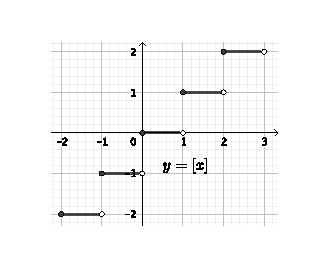
\includegraphics[scale=1,max width=\linewidth,max height=.72\textheight]{math1v3-3.pdf}
\end{minipage}
\begin{minipage}{0.55\textwidth}
$y=[x]$ функцийн графикийг харвал $x$ нь 1 рүү зүүн талаас ойртоход $[x]$ нь $0$ рүү,
баруун талаас ойртоход $1$ рүү ойртох тул ямар ч нэг тоо руу ойртохгүй.
Өөрөөр хэлбэл хязгаар оршин байхгүй (Теорем \ref{no limit condition}).
\end{minipage}
\end{example}
\end{frame}

\begin{frame}[allowframebreaks]{Функцийн хязгаарын тодорхойлолт}
\begin{example}[Хязгаар шалгах]
$\lim\limits_{x\to 1}(3x+1)\neq 7$: $\varepsilon=1$ авъя. Дурын $\delta>0$-д $x=1+\tfrac12\min(\delta,1)$ гэвэл
$0<|x-1|<\delta$ ба $3x+1\le5.5$ тул $|3x+1-7|\ge1.5>\varepsilon$.
\end{example}
\end{frame}

\begin{frame}[allowframebreaks]{Функцийн хязгаарын тодорхойлолт}
\begin{example}[Хязгаар батлах]
$\lim\limits_{x\to 1}(3x+1)=4$: $|3x+1-4|=3|x-1|$ тул $\delta=\dfrac\varepsilon3$ гэж авбал
$0<|x-1|<\delta$ үед $|3x+1-4|<\varepsilon$.
\end{example}
\end{frame}

\begin{frame}[allowframebreaks]{Функцийн хязгаарын тодорхойлолт}
\begin{example}[Төгсгөлгүйд тэмүүлэх үеийн хязгаар]
$\lim\limits_{x\to -\infty} \dfrac{x}{x+1} = 1$: $\left|\dfrac{x}{x+1}-1\right|=\dfrac{1}{|x+1|}$.
$x<-1$ үед $|x+1|=-x-1$ тул $M=-1-\dfrac1\varepsilon$ гэж авбал $x<M$ үед
$-x-1>\dfrac1\varepsilon$, иймд $\dfrac{1}{|x+1|}<\varepsilon$.
\end{example}
\end{frame}

\subsection{Хязгаар оршин байх тухай}
\begin{frame}[allowframebreaks]{Хязгаар оршин байх тухай}
\begin{theorem}[Баруун, зүүн хязгаар ба ердийн хязгаарын хамаарал]\label{casual and onesided limit}
\begin{enumerate}
\item Хэрэв $\lim\limits_{x\to a}f(x)=E$ бол $$\lim\limits_{x\to a+}f(x)=\lim\limits_{x\to a-}f(x)=E$$ байна.
\item Хэрэв $\lim\limits_{x\to a+}f(x)=\lim\limits_{x\to a-}f(x)=E$ бол $\lim\limits_{x\to a}f(x)=E$ байна.
\end{enumerate}
\end{theorem}
\end{frame}

\begin{frame}[allowframebreaks]{Хязгаар оршин байх тухай}
\begin{theorem}\label{no limit condition}
Хэрэв $\lim\limits_{x\to a+}f(x)\neq \lim\limits_{x\to a-}f(x)$ бол $\lim\limits_{x\to a}f(x)$ хязгаар оршин байхгүй.
\end{theorem}
\end{frame}

\begin{frame}[allowframebreaks]{Хязгаар оршин байх тухай}
\begin{theorem}[Хязгаар ганц байх тухай]\label{uniqlim}
Хэрэв $\lim\limits_{x\to a}f(x)$ хязгаар оршин байвал цор ганц байна.
\end{theorem}
\end{frame}

\begin{frame}[allowframebreaks]{Хязгаар оршин байх тухай}
\begin{theorem}[Хязгаарын энгийн чанарууд]\label{conslim}
\begin{enumerate}
\item $\lim\limits_{x\to a}c=c$.
\item $\lim\limits_{x\to a}x=a$.
\item Хэрэв $\lim\limits_{x\to a}f(x)=\infty$ бол $\lim\limits_{x\to a}\dfrac{1}{f(x)}=0$ байна.
\end{enumerate}
\end{theorem}
\end{frame}

% Семинар ба гэрийн даалгавар (Берманы бодлогын хураамжаас)
% Лекц 6: семинар ба гэрийн даалгавар. Бодлогууд: Г.Н. Берман, "Сборник задач по курсу
% математического анализа" (22-р хэвлэл). [Б.N] нь номын бодлогын дугаар.

\ProblemSet{Семинар 6}
\begin{frame}[allowframebreaks]{Семинар 6}
\pgroup{Хязгаарын тодорхойлолт ($\varepsilon$--$\delta$ хэлээр).}
\begin{plist}
\prob{190}{$y=x^2$. $x\to2$ үед $y\to4$. $|x-2|<\delta$-аас $|y-4|<\varepsilon=0{,}001$ мөрдөхийн тулд $\delta$ ямар байх вэ?}
\prob{192}{$y=\frac{x-1}{2(x+1)}$. $x\to3$ үед $y\to\frac14$. $|x-3|<\delta$-аас $\bigl|\frac14-y\bigr|<0{,}01$ мөрдөх $\delta$-г ол.}
\prob{193}{$x\to\frac{\pi}{2}$ үед $\sin x\to1$ болохыг батал. $1-\sin x<0{,}01$ байхын тулд $x$ нь $\frac{\pi}{2}$ цэгийн орчимд ямар нөхцөл хангах ёстой вэ?}
\prob{194}{$\displaystyle\lim_{x\to\infty}\frac{1}{x^2+1}=0$. $|x|>N$-ээс $y<\varepsilon$ мөрдөхийн тулд $N$ ямар байх вэ?}
\prob{195}{$x\to+\infty$ үед $y=\frac{x^2-1}{x^2+3}\to1$. $|x|>N$-ээс $|y-1|<\varepsilon$ мөрдөх $N$-г ол.}
\prob{213}{$x\to0$ үед $y=\frac{x}{x+1}\to0$ болохыг батал. $|y|<10^{-4}$ байхын тулд $x$ ямар нөхцөл хангах вэ?}
\prob{214}{$x\to+\infty$ үед $y=\sqrt{x+1}-\sqrt x\to0$ болохыг харуул. $x>N$ үед $y<\varepsilon$ байхын тулд $N$ ямар байх вэ?}
\end{plist}
\pgroup{Төгсгөлгүй их функц.}
\begin{plist}
\prob{198}{$x\to0$ үед $y=\frac{1+2x}{x}\to\infty$. $|y|>10^4$ байхын тулд $x$ ямар нөхцөл хангах вэ?}
\prob{199}{$x\to3$ үед $y=\frac{x}{x-3}$ төгсгөлгүй их болохыг батал. $|y|>1000$ байхын тулд $x$ ямар байх вэ?}
\prob{200}{$x\to1$ үед $y=\frac{1}{(x-1)^2}$ хязгааргүй өснө. $|x-1|<\delta$-аас $\frac{1}{(x-1)^2}>N=10^4$ мөрдөх $\delta$-г ол.}
\end{plist}
\pgroup{Хязгаарыг ол.}
\begin{plist}
\prob{268}{$\displaystyle\lim_{x\to2}\frac{x^2+5}{x^2-3}$}
\prob{272}{$\displaystyle\lim_{x\to1}\frac{x^2-2x+1}{x^3-x}$}
\prob{274}{$\displaystyle\lim_{x\to1}\frac{(x-1)\sqrt{2-x}}{x^2-1}$}
\prob{275}{$\displaystyle\lim_{x\to\frac12}\frac{8x^3-1}{6x^2-5x+1}$}
\prob{276}{$\displaystyle\lim_{x\to1}\frac{x^3+x-2}{x^3-x^2-x+1}$}
\prob{277}{$\displaystyle\lim_{x\to1}\Bigl(\frac{1}{1-x}-\frac{3}{1-x^3}\Bigr)$}
\prob{281}{$\displaystyle\lim_{x\to\infty}\frac{x^3+x}{x^4-3x^2+1}$}
\prob{283}{$\displaystyle\lim_{x\to\infty}\frac{x^2-1}{2x^2+1}$}
\prob{293}{$\displaystyle\lim_{x\to0}\frac{\sqrt{1+x^2}-1}{x}$}
\prob{296}{$\displaystyle\lim_{x\to5}\frac{\sqrt{x-1}-2}{x-5}$}
\end{plist}
\end{frame}

\ProblemSet{Гэрийн даалгавар 6}
\begin{frame}[allowframebreaks]{Гэрийн даалгавар 6}
\pgroup{Хязгаарын тодорхойлолт, төгсгөлгүй их ба зааглагдсан функц.}
\begin{plist}
\prob{191}{$y=\frac{x^2-1}{x^2+1}$. $x\to2$ үед $y\to\frac35$. $|x-2|<\delta$-аас $\bigl|y-\frac35\bigr|<0{,}1$ мөрдөх $\delta$-г ол.}
\prob{201}{$x\to0$ үед $y=\frac{1}{2^x-1}$ төгсгөлгүй их. $|y|>100$ байхын тулд $x$ ямар тэнцэтгэл биш хангах вэ?}
\prob{202}{$x\to+\infty$ үед $y=\lg x\to+\infty$. $x>M$-ээс $y>N=100$ мөрдөхийн тулд $M$ ямар байх вэ?}
\prob{204}{$y=\frac{x^2}{1+x^4}$ функц бүх тоон шулуун дээр зааглагдсан болохыг батал.}
\prob{205}{$y=\frac{x^2}{1+x^5}$ функц бүх тоон шулуун дээр зааглагдсан уу? $(0,+\infty)$ завсарт зааглагдсан уу?}
\prob{210}{Төгсгөлгүй их функц мөн үү: 1) $f(x)=x\arctg x$, \ $x\to\infty$; \ 2) $f(x)=(2+\sin x)\lg x$, \ $x\to+\infty$; \ 3) $f(x)=(1+\sin x)\lg x$, \ $x\to+\infty$?}
\prob{215}{$x\to\infty$ үед $f(x)$-ийн хязгаар $a$ бол $f(x)=a+\varphi(x)$ ($\varphi$ нь $x\to\infty$ үед төгсгөлгүй бага) хэлбэрт бичигдэхийг батал. $y=\frac{x^3}{x^3-1}$, \ $y=\frac{x^2}{2x^2+1}$, \ $y=\frac{1-x^2}{1+x^2}$-г ийм хэлбэрт бич.}
\end{plist}
\pgroup{Хязгаарыг ол.}
\begin{plist}
\prob{269}{$\displaystyle\lim_{x\to0}\Bigl(\frac{x^3-3x+1}{x-4}+1\Bigr)$}
\prob{270}{$\displaystyle\lim_{x\to1}\frac{x}{1-x}$}
\prob{271}{$\displaystyle\lim_{x\to\sqrt3}\frac{x^2-3}{x^4+x^2+1}$}
\prob{273}{$\displaystyle\lim_{x\to-2}\frac{x^3+3x^2+2x}{x^2-x-6}$}
\prob{278}{$\displaystyle\lim_{x\to2}\Bigl[\frac{1}{x(x-2)^2}-\frac{1}{x^2-3x+2}\Bigr]$}
\prob{279}{$\displaystyle\lim_{x\to1}\Bigl[\frac{x+2}{x^2-5x+4}+\frac{x-4}{3(x^2-3x+2)}\Bigr]$}
\prob{280}{$\displaystyle\lim_{x\to1}\frac{x^m-1}{x^n-1}$ \ ($m,n$ бүхэл)}
\prob{282}{$\displaystyle\lim_{x\to\infty}\frac{x^4-5x}{x^2-3x+1}$}
\prob{284}{$\displaystyle\lim_{x\to\infty}\frac{1+x-3x^3}{1+x^2+3x^3}$}
\prob{285}{$\displaystyle\lim_{x\to\infty}\Bigl(\frac{x^3}{x^2+1}-x\Bigr)$}
\prob{286}{$\displaystyle\lim_{x\to\infty}\Bigl(\frac{x^3}{2x^2-1}-\frac{x^2}{2x+1}\Bigr)$}
\prob{287}{$\displaystyle\lim_{x\to\infty}\Bigl[\frac{3x^2}{2x+1}-\frac{(2x-1)(3x^2+x+2)}{4x^2}\Bigr]$}
\prob{294}{$\displaystyle\lim_{x\to0}\frac{\sqrt{1+x}-1}{x^2}$}
\prob{295}{$\displaystyle\lim_{x\to0}\frac{\sqrt{x^2+1}-1}{\sqrt{x^2+16}-4}$}
\prob{297}{$\displaystyle\lim_{x\to1}\frac{x^2-\sqrt x}{\sqrt x-1}$}
\prob{298}{$\displaystyle\lim_{h\to0}\frac{\sqrt{x+h}-\sqrt x}{h}$}
\prob{299}{$\displaystyle\lim_{x\to0}\frac{\sqrt[3]{1+x^2}-1}{x^2}$}
\prob{300}{$\displaystyle\lim_{x\to0}\frac{\sqrt[3]{1+x}-\sqrt[3]{1-x}}{x}$}
\prob{301}{$\displaystyle\lim_{x\to a}\frac{\sqrt{x-b}-\sqrt{a-b}}{x^2-a^2}$ \ ($a>b$)}
\prob{302}{$\displaystyle\lim_{x\to1}\frac{\sqrt[n]{x}-1}{\sqrt[m]{x}-1}$ \ ($n,m$ бүхэл)}
\prob{306}{$\displaystyle\lim_{x\to\infty}\bigl(\sqrt{x+a}-\sqrt x\bigr)$}
\prob{307}{$\displaystyle\lim_{x\to\infty}\bigl(\sqrt{x^2+1}-\sqrt{x^2-1}\bigr)$}
\prob{309}{$\displaystyle\lim_{x\to\pm\infty}x\bigl(\sqrt{x^2+1}-x\bigr)$ \ ($+\infty$ ба $-\infty$-г тусад нь)}
\end{plist}
\end{frame}

% Лекц 7. Хязгаарын тухай теоремүүд
% Эх: latex/lectures/lec07-limit-2.tex (scripts/latex_to_beamer.py-ээр хөрвүүлсэн)
% Frame бүр слайдад нэг (эсвэл allowframebreaks-аар хэд хэдэн) хуудас болно;
% хэвлэх хувилбарт frame-ийн хил харагдахгүй, текст үргэлжилсэн байна.

\MathLecture{7}{Хязгаарын тухай теоремүүд}

\begin{frame}[allowframebreaks]{Хязгаарын тухай теоремүүд}
\noindent Өнөөдрийн хичээлээр бид дараалалын хязгаарын тодорхойлолт, жишээ болон функцийн хязгаарын гол чанаруудтай танилцана. Эдгээр чанарууд нь өрөөсгөл хязгаар болон төгсгөлгүйд тэмүүлэх үед ч мөн адил үнэн байдаг.
\end{frame}

\section{Дарааллын хязгаар}
\begin{frame}[allowframebreaks]{Дарааллын хязгаар}
Дараалал нь $f:\N\to\R$ функц тул  $x\to+\infty$ үед л хязгаар тодорхойлогдох боломжтой.\,
\end{frame}

\begin{frame}[allowframebreaks]{Дарааллын хязгаар}
\begin{definition}[Дараалалын хязгаар]
 $ a_1, a_2, a_3, \ldots, a_n, \ldots$ бодит тоон дараалал байг. \\
Хэрэв дурын $\varepsilon>0$  тоо авах бүрт  
$$n>\delta \text{ байх бүх } n \text{ натурал тооны хувьд } |a_n-E|<\varepsilon$$
нөхцлийг хангах $\delta>0$ тоо олдож байвал $E$ тоог $a_n$ дараалалын  хязгаар гээд $$\lim\limits_{n\to  \infty}a_n=E$$ гэж бичнэ.   Хэрэв дараалал төгсгөлөг $E$ хязгаартай бол нийлдэг дараалал, бусад үед сарнидаг дараалал гэнэ.
\end{definition} 
\end{frame}

\begin{frame}[allowframebreaks]{Дарааллын хязгаар}
\begin{example}[Төгсгөлөг хязгаартай дараалал]
$a_n = \dfrac{n}{n+1}$ дараалал өгөгдөв.  \[
\lim_{n\to\infty}\frac{n}{n+1}=1.
\] харуулая.
\[
\frac{n}{n+1}=1-\frac{1}{n+1}
\]  байна.
Дурын $\varepsilon>0$ хувьд $\delta=\frac{1}{\varepsilon}$ гэе. Хэрэв $n>1+\delta=\frac{1}{\varepsilon}+1>\dfrac{1}{\varepsilon}$ бол $\dfrac{1}{n+1}<\varepsilon$ байна. Иймд 
\[
\left|\frac{n}{n+1}-1\right| =\left|\frac{n-(n+1)}{n+1}\right|=\frac{1}{n+1}< \varepsilon.
\]
Иймд
\[
\lim_{n\to\infty}\frac{n}{n+1}=1
\] батлагдав.
\end{example}
\end{frame}

\begin{frame}[allowframebreaks]{Дарааллын хязгаар}
\begin{example}[Төгсгөлгүй рүү тэмүүлэх дараалал]
$a_n = n$ дараалал өгөгдөв.  
Дурын $M>0$ бодит тоонд $\delta=M$ гэж авъя. Тэгвэл $n>\delta$ үед $a_n=n>M$.  
Иймд
\[
\lim_{n\to\infty} n = +\infty.
\]
\end{example}
\end{frame}

\begin{frame}[allowframebreaks]{Дарааллын хязгаар}
\begin{example}[Хязгаар оршдоггүй дараалал]
$a_n = (-1)^n$ дараалал нь 
\[
\lim_{n\to\infty} (-1)^n \quad \text{оршихгүй}.
\]
\end{example}
\begin{prof}
Эсрэгээр нь $\{a_n\}$ дараалалын хязгаар $L\in\mathbb{R}$ оршино гэж үзье. 
Нийлэхийн тодорхойлолтоор дурын $\varepsilon>0$ тооны хувьд $\exists\,N\in\mathbb{N}$ ба $n>N$ үед 
\[
|a_n-L|<\varepsilon
\]
байх ёстой.

Одоо $\varepsilon=1$ гэж авъя. Тэгвэл $\exists\,N$, $n>N$ үед $|a_n-L|<1$ байх ёстой.
 $a_n$-ийн тэгш ба сондгой индексүүдийг ялгаж авч үзье:
\[
a_{2k}=1,\qquad a_{2k+1}=-1\quad (k\in\mathbb{N}).
\]
\textbf{(i) Хэрэв $L> 0$} бол сондгой бүх $n> N$-д $a_n=-1$ тул
\[
|a_n-L|=|-1-L|=1+L\ge 1,
\]
ингэснээр $|a_n-L|<1$ нөхцөл зөрчлөгдөнө.

\textbf{(ii) Хэрэв $L\le 0$} бол тэгш бүх $n> N$-д $a_n=1$ тул
\[
|a_n-L|=|1-L|=1-L\ge 1,
\]
дахиад л $|a_n-L|<1$ нөхцөл зөрчинө.

Харин \textbf{$L$ нь $>0$ эсвэл $\le 0$ хоёрын нэг} байх тул аль ч тохиолдолд зөрчил гарч байна. 
Иймээс анхны таамаг (\(L\) хязгаар оршино) буруу. Тэгэхээр
\[
\lim_{n\to\infty}(-1)^n \ \text{оршихгүй}.
\]
\end{prof}
\end{frame}

\begin{frame}[allowframebreaks]{Дарааллын хязгаар}
\begin{theorem}[Хязгаар ганц байх тухай]\label{uniqlim}
$f:X\to\R$ функц, $x\to a$ байг. Хэрэв $\displaystyle\lim_{x\to a} f(x)$ хязгаар оршин байвал цор ганц байна. Өөрөөр хэлбэл хэн, хаана, ямар аргаар бодсон ч ижил утгатай.
\end{theorem}

\begin{prof}
Эсрэгээр нь $\lim_{x\to a}f(x)=b_1$ болон $\lim_{x\to a}f(x)=b_2$ гэсэн хоёр өөр хязгаар ($b_1>b_2$) оршин байдаг гэж үзье.

$\varepsilon=\dfrac{b_1-b_2}{3}$ авбал $b_2+\varepsilon=b_1-2\varepsilon<b_1-\varepsilon$ байна. Иймд $\emptyset=(b_1-\varepsilon, b_1+\varepsilon)\cap (b_2-\varepsilon,b_2+\varepsilon)$ болов.

Хязгаарын тодорхойлолтоор $\exists\,\delta_1>0$ ба, $|x-a|<\delta_1$ үед $|f(x)-b_1|<\varepsilon$; мөн $\exists\,\delta_2>0$ ба, $|x-a|<\delta_2$ үед $|f(x)-b_2|<\varepsilon$. $|x_0-a|<\min(\delta_1,\delta_2)$ бүхий $x_0$ сонговол
\[
b_2-\varepsilon<f(x_0)<b_2+\varepsilon<b_1-\varepsilon<f(x_0)<b_1+\varepsilon,
\]
гэж зөрчил гарна. Иймд $b_1=b_2$.
\end{prof}
\end{frame}

\begin{frame}[allowframebreaks]{Дарааллын хязгаар}
\begin{theorem}[Хязгаарын энгийн чанарууд]\label{conslim}
$c,a$ тогтмол тоонууд, $x\to a$ байг. Дараах тэнцэтгэлүүд үнэн:
\begin{description}[leftmargin=2em]
  \item[(P1)] $\displaystyle\lim_{x\to a} c = c$,
  \item[(P2)] $\displaystyle\lim_{x\to a} x = a$.
\end{description}
\end{theorem}

\begin{prof}
(P1) $f(x)\equiv c$. Дурын $\varepsilon>0$ үед ямар ч $\delta>0$ дээр $|f(x)-c|=0<\varepsilon$, тиймээс $\lim_{x\to a}c=c$.

(P2) $f(x)=x$. Дурын $\varepsilon>0$ үед $\delta=\varepsilon$ гэж авбал $|x-a|<\delta$ үед $|f(x)-a|=|x-a|<\varepsilon$, тиймээс $\lim_{x\to a}x=a$.
\end{prof}
\end{frame}

\begin{frame}[allowframebreaks]{Дарааллын хязгаар}
\begin{theorem}[Хязгаар ба үйлдлүүд]\label{aritlim}
$f,g:X\to\R$, $x\to a$, $A,B,C\in\R$ байг. Хэрэв $$\displaystyle\lim_{x\to a} f(x)=A \text{ ба } \displaystyle\lim_{x\to a} g(x)=B$$ бол:
\begin{description}[leftmargin=2em]
  \item[(P3)] $f$ нь $(a-p,a+p)\cap X$ олонлог дээр зааглагдсан байх  $\exists\,p>0$;
  \item[(P4)] $\displaystyle\lim_{x\to a}f(x)\pm g(x)=A\pm B$;
  \item[(P5)] $\displaystyle\lim_{x\to a} C\,g(x)=CB$, \quad $\displaystyle\lim_{x\to a} f(x)g(x)=AB$;
  \item[(P6)] Хэрэв $B\neq 0$ бол $\displaystyle\lim_{x\to a}\dfrac{f(x)}{g(x)}=\dfrac{A}{B}$.
\end{description}
\end{theorem}

\begin{prof}
(P3) Хязгаар оршин байвал $\exists\,p>0$ ба, $|x-a|<p$ үед $|f(x)-A|<1$ болно. Иймээс $A-1<f(x)<A+1$ болж $(a-p,a+p)\cap X$ дээр зааглагдсан.

(P4) Хязгаарын тодорхойлолтоор:
\begin{align*}
&\forall\,\varepsilon_1>0,\;\exists\,\delta_1>0\text{ тийм, }|x-a|<\delta_1\Rightarrow |f(x)-A|<\varepsilon_1,\\
&\forall\,\varepsilon_2>0,\;\exists\,\delta_2>0\text{ тийм, }|x-a|<\delta_2\Rightarrow |g(x)-B|<\varepsilon_2.
\end{align*}

Дурын $\varepsilon>0$ өгөгдсөн байг.  
Бид $\varepsilon_1=\varepsilon_2=\dfrac{\varepsilon}{2}$ гэж авъя.

Тэгвэл:
\[
|f(x)-A|<\frac{\varepsilon}{2},\qquad |g(x)-B|<\frac{\varepsilon}{2}.
\]
Одоо $\delta=\min(\delta_1,\delta_2)$ гэж авбал $|x-a|<\delta$ үед дээрх хоёр тэнцэтгэл биш хоёулаа биелнэ.  
Тэгвэл
\begin{align*}
|(f(x)\pm g(x))-(A\pm B)|
&=|(f(x)-A)\pm(g(x)-B)|\\
&\le |f(x)-A|+|g(x)-B|\\
&<\frac{\varepsilon}{2}+\frac{\varepsilon}{2}=\varepsilon.
\end{align*}
Иймд хязгаарын тодорхойлолтоор
\[
\lim_{x\to a}\bigl(f(x)\pm g(x)\bigr)=A\pm B.
\]

(P5) Эхлээд $\displaystyle\lim_{x\to a}\bigl(f(x)-A\bigr)\bigl(g(x)-B\bigr)=0$ гэж харуулъя. Дурын $\varepsilon>0$ хувьд $\delta_1,\delta_2>0$ олдоод $|x-a|<\delta_1\Rightarrow |f(x)-A|<\sqrt{\varepsilon}$, $|x-a|<\delta_2\Rightarrow |g(x)-B|<\sqrt{\varepsilon}$ байна. Тэгвэл $|x-a|<\min(\delta_1,\delta_2)$ үед 
$|(f(x)-A)(g(x)-B)|=|f(x)-A||g(x)-B|<\sqrt{\varepsilon}\sqrt{\varepsilon}=\varepsilon$ болно.

Одоо
\[
f(x)g(x)=(f(x)-A)(g(x)-B)+A\,g(x)+B\,f(x)-AB
\]
гэж бичээд (P4), (P5)-ийн эхний хэсгийг хэрэглэвэл 
\begin{align*}
\lim_{x\to a}f(x)g(x)&=\lim_{x\to a}\left((f(x)-A)(g(x)-B)+A\,g(x)+B\,f(x)-AB\right)\\
&=\lim_{x\to a}((f(x)-A)(g(x)-B)+\lim_{x\to a}A\,g(x)+\lim_{x\to a} B\,f(x)-AB\\
&=0+AB+AB-AB=AB
.
\end{align*}

(P6)  Бидэнд $B\neq 0$ тул $|B|>0$.  
$\displaystyle\lim_{x\to a}g(x)=B$ гэсэн тодорхойлолтоор $\exists\,\delta_1>0$ ба, $|x-a|<\delta_1$ үед
\[
|g(x)-B|<\frac{|B|}{2}.
\]
Тэгвэл 
\[
|g(x)|\ge |B|-|g(x)-B|>\frac{|B|}{2},
\]
өөрөөр хэлбэл $x$ нь $a$-д ойрхон үед $g(x)$ тэг болохгүй.

Одоо дурын $\varepsilon>0$ авъя.  
$\displaystyle\lim_{x\to a}f(x)=A$ ба $\displaystyle\lim_{x\to a}g(x)=B$ учраас $\exists\,\delta_2,\delta_3>0$ ба хэрэв $|x-a|<\delta_2$ бол
\[
|f(x)-A|<\frac{\varepsilon |B|}{4},
\]
мөн хэрэв $|x-a|<\delta_3$ бол
\[
|g(x)-B|<\min\left(\frac{|B|}{2},\,\frac{\varepsilon |B|^2}{4(|A|+1)}\right).
\]
Одоо $\delta=\min(\delta_1,\delta_2,\delta_3)$ гэж авъя. Тэгвэл $|x-a|<\delta$ үед дараах үнэлгээ биелнэ:
\begin{align*}
\left|\frac{f(x)}{g(x)}-\frac{A}{B}\right|
&=\left|\frac{f(x)B-A g(x)}{g(x)B}\right|
=\frac{|B(f(x)-A)-A(g(x)-B)|}{|g(x)B|}\\[4pt]
&\le \frac{|B||f(x)-A|+|A||g(x)-B|}{|g(x)||B|}.
\end{align*}
Бид $|g(x)|>\frac{|B|}{2}$ гэдгийг дээр баталсан тул
\[
\left|\frac{f(x)}{g(x)}-\frac{A}{B}\right|
<\frac{2}{|B|}\Big(|f(x)-A|+\frac{|A|}{|B|}|g(x)-B|\Big).
\]

Одоо $|x-a|<\delta$ үед $|f(x)-A|<\frac{\varepsilon |B|}{4}$, $|g(x)-B|<\frac{\varepsilon |B|^2}{4(|A|+1)}$ тул
\[
\left|\frac{f(x)}{g(x)}-\frac{A}{B}\right|
<\frac{2}{|B|}\!\left(\frac{\varepsilon |B|}{4}+\frac{|A|}{|B|}\cdot\frac{\varepsilon |B|^2}{4(|A|+1)}\right)
=\varepsilon\left(\frac12+\frac{|A|}{2(|A|+1)}\right)
<\varepsilon.
\]
Иймд хязгаарын тодорхойлолтоор
\[
\lim_{x\to a}\frac{f(x)}{g(x)}=\frac{A}{B}.
\]
\end{prof}
\end{frame}

\begin{frame}[allowframebreaks]{Дарааллын хязгаар}
\begin{theorem}[Хязгаар ба тэнцэтгэл биш]\label{ineqlim}
\begin{enumerate}[label=(\arabic*)]
\item Хэрэв $x\in (a-\delta,a+\delta)$-н хувьд $h(x)\ge 0$ ба $\lim_{x\to a} h(x)=A$ бол $A\ge 0$.
\item Хэрэв $x\in (a-\delta,a+\delta)$-н хувьд $f(x)\le g(x)$ ба $\lim_{x\to a} f(x)$, $\lim_{x\to a} g(x)$ оршидог бол 
\[
\lim_{x\to a} f(x)\le \lim_{x\to a} g(x).
\]
\item Хэрэв $x\in (a-\delta,a+\delta)$-н хувьд $f(x)\le g(x)\le h(x)$ ба $\lim_{x\to a} f(x)=\lim_{x\to a} h(x)=A$ бол
\[
\lim_{x\to a} f(x)=\lim_{x\to a} g(x)=\lim_{x\to a} h(x)=A.
\]
\end{enumerate}
\end{theorem}

\begin{prof}
(1) Эсрэгээр нь $A<0$ гэе. Тэгвэл $A+\varepsilon<0$ байх $\varepsilon$ авч үзье. Тодорхойлолт ёсоор $\varepsilon>0$ хувьд $|x-a|$ хангалттай бага үед $h(x)\in (A-\varepsilon,A+\varepsilon)\subset (-\infty,0)$ болно. Гэтэл $h(x)\ge 0$ тул зөрчил.

(2) $h(x)=g(x)-f(x)\ge 0$-д (1)-ийг хэрэглэвэл $\lim_{x\to a} h(x)\ge 0$, өөрөөр хэлбэл $\lim_{x\to a} g(x)-\lim_{x\to a} f(x)\ge 0$.

(3) $\lim_{x\to a} f(x)=\lim_{x\to a} h(x)$ учраас $\lim_{x\to a} (f(x)-g(x))=0$ болно. Иймд $\forall \varepsilon>0$ хувьд $\exists\delta >0$ ба  $|x-a|<\delta$ үед $|h(x)-f(x)|=h(x)-f(x)=(h(x)-g(x))+(g(x)-f(x))<\varepsilon$ байна. Энд байгаа нэмэгдэхүүн бүр эерэг байхыг санавал $h(x)-g(x)< (h(x)-g(x))+(g(x)-f(x))<\varepsilon$ ба $g(x)-f(x)< (h(x)-g(x))+(g(x)-f(x))<\varepsilon$ байна. Иймд тодорхойлолт ёсоор $0$ тоо нь  $\lim_{x\to a} h(x)-g(x)$ ба $\lim_{x\to a} g(x)-f(x)$ хязгаартай тэнцүү болж байна. Иймд '
$$\lim_{x\to a} g(x)=\lim_{x\to a} (g(x)-f(x))+f(x)=\lim_{x\to a} (g(x)-f(x))+\lim_{x\to a} f(x)=0+A$$ болж батлагдав.
\end{prof}
\end{frame}

\begin{frame}[allowframebreaks]{Дарааллын хязгаар}
\begin{theorem}[Хязгаар ба композици]\label{complim}
$f,g$ функцүүд өгөгдөж, $f\circ g$ тодорхойлогдсон байг. Хэрэв $\displaystyle\lim_{x\to a} g(x)=b$ ба $\displaystyle\lim_{z\to b} f(z)=A$ бол
\[
\lim_{x\to a} f\bigl(g(x)\bigr)=A.
\]
\end{theorem}

\begin{prof}
Дурын $\varepsilon>0$-д $\exists\,\delta_1>0$ тийм, $|z-b|<\delta_1\Rightarrow |f(z)-A|<\varepsilon$. Мөн $\exists\,\delta>0$ тийм, $|x-a|<\delta\Rightarrow |g(x)-b|<\delta_1$. Иймд $|x-a|<\delta$ үед $|f(g(x))-A|<\varepsilon$.
\end{prof}
\end{frame}

\begin{frame}[allowframebreaks]{Дарааллын хязгаар}
\begin{theorem}[Монотон дарааллын хязгаар]\label{monton seq lim}
Хэрэв дараалал монотон бөгөөд зааглагдсан бол нийлнэ.  
\begin{enumerate}
\item Өсөх ба дээрээсээ зааглагдсан дараалал төгсгөлөг хязгаартай бөгөөд нийлнэ.  
\item Буурах ба доороосоо зааглагдсан дараалал төгсгөлөг хязгаартай бөгөөд нийлнэ.
\end{enumerate}
\end{theorem}
\end{frame}

\section{Хязгаар бодох (жишээнүүд)}
\begin{frame}[allowframebreaks]{Хязгаар бодох (жишээнүүд)}
\begin{example}
$\displaystyle \lim_{x\to 2}\frac{x^2-1}{x^3+3x}$.

(P5)-оос $\lim_{x\to 2}x^2=(\lim x)^2=2^2=4$, $\lim_{x\to 2}x^3=8$, (P4)-өөс $\lim_{x\to 2}(x^2-1)=3$, харин $\lim_{x\to 2}(x^3+3x)=8+6=14$. (P6)-оор
\[
\lim_{x\to 2}\frac{x^2-1}{x^3+3x}=\frac{3}{14}.
\]
\end{example}
\end{frame}

\begin{frame}[allowframebreaks]{Хязгаар бодох (жишээнүүд)}
\begin{example}
$\displaystyle \lim_{x\to 2}\frac{x^2-2x}{x^2-4}$.

Шууд орлуулбал $\frac{0}{0}$ тул хялбарчилъя:
\[
\frac{x^2-2x}{x^2-4}=\frac{x(x-2)}{(x-2)(x+2)}=\frac{x}{x+2}\quad (x\neq 2).
\]
Тэгвэл $\displaystyle \lim_{x\to 2}\frac{x}{x+2}=\frac{2}{4}=\frac12$.
\end{example}
\end{frame}

\begin{frame}[allowframebreaks]{Хязгаар бодох (жишээнүүд)}
\begin{example}
$\displaystyle \lim_{x\to 2}\sqrt{x}$.

Хэрэв $l=\lim_{x\to 2}\sqrt{x}$ орших тул (P5)-оор $l^2=\lim x=2$, мөн $\sqrt{x}\ge 0$ тул $l=\sqrt{2}$.
\end{example}
\end{frame}

\begin{frame}[allowframebreaks]{Хязгаар бодох (жишээнүүд)}
\begin{example}\label{ininf}
Хэрэв $\displaystyle \lim_{x\to a} f(x)=+\infty$ бол $\displaystyle \lim_{x\to a}\frac{1}{f(x)}=0$.

Үнэхээр, дурын $\varepsilon>0$-д $|x-a|$ хангалттай жижиг үед $f(x)>\frac{1}{\varepsilon}>0$, тэгвэл $0<\frac{1}{f(x)}<\varepsilon$.
\end{example}
\end{frame}

\begin{frame}[allowframebreaks]{Хязгаар бодох (жишээнүүд)}
\begin{example}
$\displaystyle \lim_{x\to \infty}\frac{2x^3+5x-2}{3x^3-2x^2+x-1}$.

Хамгийн их зэрэг $x^3$ тул $x^3$-д хуваая:
\[
\frac{x^3(2+\frac{5}{x^2}-\frac{2}{x^3})}{x^3(3-\frac{2}{x}+\frac{1}{x^2}-\frac{1}{x^3})}
\ \xrightarrow[x\to\infty]{}\ \frac{2}{3}.
\]
\end{example}
\end{frame}

\begin{frame}[allowframebreaks]{Хязгаар бодох (жишээнүүд)}
\begin{example}

\begin{enumerate}[label=(\alph*)]
\item $-\dfrac{\pi}{2}<x<\dfrac{\pi}{2}$ үед $-x<\sin x<x$-ийг Теорем \ref{ineqlim}-д ашиглабал $\displaystyle \lim_{x\to 0}\sin x=0$ ;
\item $\displaystyle \lim_{x\to 0}\cos x=1$ ( $\sqrt{1-\sin^2x}\le \cos x\le 1$-ийг ашиглав) байна.
\end{enumerate}
\end{example}
\end{frame}

\begin{frame}[allowframebreaks]{Хязгаар бодох (жишээнүүд)}
\begin{example}[I гайхамшигт хязгаар]
\[
\lim_{x\to 0}\frac{\sin x}{x}=1
\] батлая.

$x\in(0,\tfrac{\pi}{2})$ үед нэгж тойрог дээр $O=(0,0)$, $A=(1,0)$, $B=(\cos x,\sin x)$ гэж авъя. $A$ дээрх шүргэгч $x=1$ шулуун нь $OB$ цацрагтай $C$ дээр огтлолцоно; тэгвэл $C=(1,\tan x)$.
\begin{center}
\begin{fitbox}\begin{tikzpicture}[scale=3,>=stealth]
  % өнцөг
  \def\ang{50}

  % тэнхлэг, тойрог
  \draw[->] (-0.1,0) -- (1.2,0) node[below] {$x$};
  \draw[->] (0,-0.1) -- (0,1.1) node[left] {$y$};
 

  % цэгүүд
  \coordinate (O) at (0,0);
  \coordinate (A) at (1,0);
  \coordinate (B) at ({cos(\ang)},{sin(\ang)});
  \coordinate (C) at (1,{tan(\ang)});

  % сектор (нуугдмал өнгө)
  \fill[blue!12] (O) -- (A) arc (0:\ang:1) -- cycle;

  % гурвалжин OAB (дотоод)
  \fill[green!18] (O) -- (A) -- (B) -- cycle;

  % шүргэгч ба гурвалжин OAC (гадна)
  \draw[dashed] (1,0) -- (1,1.05);
  \fill[red!12] (O) -- (A) -- (C) -- cycle;

  % ирмэгүүд
  \draw[thick] (O) -- (A) -- (B) -- cycle;
  \draw[thick] (O) -- (C);

  % өнцгийн нум ба тэмдэглэгээ
  \draw[thick] (0.25,0) arc (0:\ang:0.25);
  \node at ({0.35*cos(\ang/2)},{0.35*sin(\ang/2)}) {$x$};

  % цэгүүдийн тэмдэглэгээ
  \fill (O) circle (0.015) node[below left] {$O$};
  \fill (A) circle (0.015) node[below] {$A(1,0)$};
  \fill (B) circle (0.015) node[above right] {$B(\cos x,\sin x)$};
  \fill (C) circle (0.015) node[right] {$C(1,\tan x)$};

  % тайлбар
  \node[green!50!black] at (0.62,0.18) {$\frac12\sin x$};
  \node[blue!60!black]  at (0.45,0.35) {$\frac{x}{2}$};
  \node[red!70!black]   at (0.80,0.50) {$\frac12\tan x$};
 \draw[thick] (0,0) circle (1);
\end{tikzpicture}\end{fitbox}
\end{center}

Талбайнууд:
\[
S_{\triangle OAB}=\frac12\sin x,\qquad
S_{\text{sector }OAB}=\frac{x}{2},\qquad
S_{\triangle OAC}=\frac12\tan x.
\]
Геометрийн хувьд $\triangle OAB$ нь сектороос бага, харин сектор нь $\triangle OAC$-аас бага тул
\[
\frac12\sin x\;<\;\frac{x}{2}\;<\;\frac12\tan x
\quad\Longrightarrow\quad
\sin x\;<\;x\;<\;\tan x.
\]
Өөрөөр 
\[
\cos x<\frac{\sin x}{x}<1 \qquad (0<x<\tfrac{\pi}{2})
\] гэж бичиж болно.
$x\to 0^+$ үед $\cos x\to 1$ тул Теорем \ref{ineqlim}.3-аар $\dfrac{\sin x}{x}\to 1$. $\dfrac{\sin x}{x}$ нь тэгш ($\sin(-x)/(-x)=\sin x/x$) тул $x\to 0-$ үед ч ижил дүгнэлт гарч,
\[
\lim_{x\to 0}\frac{\sin x}{x}=1.
\] Энэ хязгаарыг “I гайхамшигт хязгаар” гэж нэрлэдэг.
\end{example}
\end{frame}

\begin{frame}[allowframebreaks]{Хязгаар бодох (жишээнүүд)}
\begin{example}
    $(1+\dfrac{1}{2n})^n<2$ батал.

Бид семинар дээр $a>b>0$ ба $k\in\mathbb{N}$ бол 
\[
a^k \;<\;b^k+ k\,a^{\,k-1}(a-b)
\] байдгийг баталсан. Энд $a=1+\dfrac{1}{2n}  \;, \; b=1 \;, \;k=n+1$ гэвэл \[
\bigl( 1+\dfrac{1}{2n}\bigr) ^{\,n+1} \;<\; 1+(n+1)\,\bigl(1+\dfrac{1}{2n}\bigr)^{\,n}\Bigl(1+\dfrac{1}{2n}-1\Bigr)=1+(n+1)\,\bigl(1+\dfrac{1}{2n}\bigr)^{\,n}\cdot \frac{1}{2n}.
\]
Ингээд
\[
\bigl( 1+\dfrac{1}{2n}\bigr) ^{\,n+1}-(n+1)\,\bigl(1+\dfrac{1}{2n}\bigr)^{\,n}\cdot \frac{1}{2n}=\bigl(1+\dfrac{1}{2n}\bigr)^{\,n}\Bigl[1+\dfrac{1}{2n}-\dfrac{n+1}{2n}\Bigr] =\dfrac{1}{2}\bigl(1+\dfrac{1}{2n}\bigr)^{\,n}<1
\]
болно. Иймээс
\[
\Bigl(1+\frac{1}{2n}\Bigr)^{n} \;<\;2.
\]
батлагдав.
\end{example}
\end{frame}

\begin{frame}[allowframebreaks]{Хязгаар бодох (жишээнүүд)}
\begin{example}
    $\bigl(1+\dfrac{1}{n}\bigr)^n<\bigl(1+\dfrac{1}{n+1}\bigr)^{n+1}$ батал.

Өмнөх тэнцэтгэл бишид $a=1+\dfrac{1}{n}  \;, \; b=1\dfrac{1}{n+1} \;, \;k=n+1$ гэвэл батлагданa. 
\end{example}
\end{frame}

\begin{frame}[allowframebreaks]{Хязгаар бодох (жишээнүүд)}
\begin{example}[II гайхамшигт хязгаар]
     $\lim\limits_{n\to\infty}\Bigl(1+\dfrac{1}{n}\Bigr)^n$ дараалал нийлэхийг батал.

Өмнөх жишээнүүдээс $$4>(1+\dfrac{1}{2n})^{2n}>(1+\dfrac{1}{2n-1})^{2n-1}$$ гарах тул $\Bigl(1+\dfrac{1}{n}\Bigr)^n$ дараалал өсдөг дээрээсээ зааглагдсан дараалал байна. Иймд Теорем \ref{monton seq lim}-ээр хязгаартай. Энэ дараалалын хязгаарыг $e$ гэж нэрлэдэг.  $e\approx 2.7182818\dots$ байдаг.
     Энэ хязгаарыг “II гайхамшигт хязгаар” гэж нэрлэдэг.
\end{example}
\end{frame}

\section{Семинар 7}
\begin{frame}[allowframebreaks]{Семинар 7}
\begin{multicols}{2}
\begin{enumerate}
\item $\displaystyle \lim_{x\to -1} \frac{x^{2}-1}{x^{2}+3x+2}.$
\item $\displaystyle \lim_{x\to 5} \frac{x^{2}-25}{x-5}.$
\item $\displaystyle \lim_{x\to 2} \frac{x^{2}-5x+6}{x^{2}-12x+20}.$
\item $\displaystyle \lim_{x\to 1} \frac{2x^{3}-2x^{2}+x-1}{x^{3}-x^{2}+3x-3}.$
\item $\displaystyle \lim_{x\to -1} \frac{2x^{3}+2x^{2}+3x+3}{x^{3}+x^{2}+x+1}.$
\item $\displaystyle \lim_{x\to -3} \frac{x^{3}+5x^{2}+3x-9}{x^{3}+8x^{2}+21x+18}.$
\item $\displaystyle \lim_{x\to 0} \frac{x^{4}+x^{3}}{x^{4}-2x^{3}}.$
\item $\displaystyle \lim_{x\to a} \frac{x^{2}-(a+1)x+a}{x^{3}-a^{3}}.$
\item $\displaystyle \lim_{x\to 1} \Big(\frac{1}{1-x}-\frac{2}{1-x^{2}}\Big).$
\item $\displaystyle \lim_{x\to 0} \frac{\sqrt{x^{2}+1}-1}{\sqrt{x^{2}+16}-4}.$
\item $\displaystyle \lim_{x\to 0} \frac{\sqrt{1+x}-\sqrt{1-x}}{x}.$
\item $\displaystyle \lim_{h\to 0} \frac{\sqrt{x+h}-\sqrt{x}}{h}.$
\item $\displaystyle \lim_{x\to \infty} \big(\sqrt{x^{2}+1}-\sqrt{x^{2}-1}\big).$
\item $\displaystyle \lim_{x\to \pm\infty} (\sqrt{x^{2}+1}-x).$
\item $\displaystyle \lim_{x\to +\infty} x\, (\sqrt{x^{2}+1}-x).$
\item $\displaystyle \lim_{x\to 0} \frac{\sqrt[3]{1+x}-\sqrt[3]{1-x}}{x}.$
\item $\displaystyle \lim_{h\to 0} \frac{\sqrt[3]{x+h}-\sqrt[3]{x}}{h}.$
\item $\displaystyle \lim_{x\to -8} \frac{\sqrt{1-x}-3}{2+\sqrt[3]{x}}.$
\item $\displaystyle \lim_{x\to +\infty} \big(\sqrt[3]{x^{3}+x^{2}+1}-\sqrt[3]{x^{3}-x^{2}+1}\big).$
\item $\displaystyle \lim_{x\to \infty} \frac{1-3x}{2x+3}.$
\item $\displaystyle \lim_{x\to \infty} \frac{10x+5}{0.01\,x^{2}-6x}.$
\item $\displaystyle \lim_{x\to \infty} \frac{x^{3}-5x+2}{x+10^{10}}.$
\item $\displaystyle \lim_{x\to \infty} \frac{2x^{2}-3x-4}{\sqrt{x^{4}+1}}.$
\item $\displaystyle \lim_{x\to \infty} \frac{\sqrt{x}}{\sqrt{x+\sqrt{x}+\sqrt[4]{x}}}.$
\item $\displaystyle \lim_{x\to \infty} \big[\sqrt[3]{(x+1)^{2}}-\sqrt[3]{(x-1)^{2}}\big].$
\item $\displaystyle \lim_{x\to \infty} \frac{(x-1)^{3}}{2x^{3}+3x+1}.$
\item $\displaystyle \lim_{x\to \infty} \frac{x^{2}-5x+1}{3x+7}.$
\item $\displaystyle \lim_{x\to \infty} \frac{x}{\sqrt[3]{x^{3}+9}}.$
\item $\displaystyle \lim_{x\to \infty} \frac{\sqrt[3]{x^{2}+1}}{x+1}.$
\item $\displaystyle \lim_{x\to 0}\frac{\sin 3x}{x}$
\item $\displaystyle \lim_{x\to 0}\frac{\tan 5x}{\sin 2x}$
\item $\displaystyle \lim_{x\to 0}\frac{\tan 2x}{\tan 3x}$
\item $\displaystyle \lim_{x\to 0}\frac{\sin 4x}{\tan 3x}$
\item $\displaystyle \lim_{x\to 0}\frac{\tan 5x}{x}$
\item $\displaystyle \lim_{x\to 0}\frac{1-\cos x}{x^{2}}$
\item $\displaystyle \lim_{x\to 0}\frac{\tan x-\sin x}{x^{3}}$
\item $\displaystyle \lim_{x\to 0}\frac{1-\cos 2x}{x^{2}}$
\item $\displaystyle \lim_{x\to 0}\frac{\ln(1+x)}{x}$
\item $\displaystyle \lim_{x\to 0}\frac{\ln(1+2x)}{x}$
\item $\displaystyle \lim_{x\to 0}\frac{\ln(1+x)-x}{x^{3}}$
\item $\displaystyle \lim_{x\to 0}\frac{e^{x}-1-x}{x^{2}}$
\item $\displaystyle \lim_{x\to 0}\frac{(1+x)^{a}-(1+x)^{b}}{x}$
\item $\displaystyle \lim_{x\to 0}\frac{(1+x)^{n}-1}{x}$
\item $\displaystyle \lim_{x\to 0}\frac{(1+7x)^{9}-1-63x}{x^{2}}$
\item $\displaystyle \lim_{x\to 0}\frac{e^{3x}-1}{x+x^{2}}$
\end{enumerate}
\end{multicols}
\end{frame}

\section*{Хязгаар сэдвийн даалгавар}
\begin{frame}[allowframebreaks]{Хязгаар сэдвийн даалгавар}
\begin{enumerate}
\item Хязгаарыг тодорхойлолтын дагуу шалга.
\begin{multicols}{2}
\begin{enumerate}
\item $\lim\limits_{x\to 2}\sqrt{x}=\sqrt{2}$ 
\item $\lim\limits_{x\to 2}(3x+5)=11$
\item $\lim\limits_{n\to +\infty}\dfrac{n^2+2n+1}{n^2+n+1}=1$
\item $\lim\limits_{n\to \infty}\dfrac{n}{n+1}=1$
\end{enumerate}
\end{multicols}
\item Хязгаарыг бод.
\begin{multicols}{2}
\begin{enumerate}
\item $\lim\limits_{x\to 1}\dfrac{x^2-1}{x-1}$
\item $\lim\limits_{x\to 4}\dfrac{\sqrt{x}-2}{x-4}$
\item $\lim\limits_{x\to \infty}\dfrac{3x^2+2}{5x^2-7}$
\item $\lim\limits_{x\to \infty}\dfrac{\sqrt{x^2+3}}{x}$
\item $\lim\limits_{x\to 0^+}\dfrac{1}{x}$
\item $\lim\limits _{x\to 1} \dfrac{x^{n+1}-(n+1)x+n}{(x-1)^2}$ 
\item $\lim\limits _{x\to 1} \dfrac{m}{1-x^m}-\dfrac{n}{1-x^n}$
\item $\lim\limits _{x\to +\infty} \dfrac{\sqrt{x+\sqrt{x+\sqrt{x}}}}{\sqrt{x+1}}$
\item $\lim\limits _{x\to +\infty} \dfrac{\sqrt{x}+\sqrt[3]{x}+\sqrt[4]{x}}{\sqrt{2x+1}}$ 
\item $\lim\limits _{x\to 4} \dfrac{\sqrt{1+2x}-3}{\sqrt{x}-2}$
\item $\lim\limits _{x\to 8} \dfrac{\sqrt{1+x}-3}{\sqrt[3]{x}-2}$
\item $\lim\limits_{x\to \infty}\dfrac{2x+3}{5x-1}$
\item $\lim\limits_{x\to -\infty}\dfrac{x^2+1}{2x^2-3}$
\item $\lim\limits_{x\to \infty}\dfrac{2x^3-1}{x^3+5}$
\item $\lim\limits_{x\to 0}\dfrac{\sqrt{1+x}-1}{x}$
\item $\lim\limits_{x\to 0}\dfrac{\ln(1+2x)}{x}$
\item $\lim\limits_{x\to \infty}\dfrac{\sqrt{x^2+5x}}{x}$
\end{enumerate}
\end{multicols}
\item I гайхамшигт хязгаар хэрэглэн хязгаарыг бод.
\begin{multicols}{2}
\begin{enumerate}
\item $\lim\limits_{x\to 0}\dfrac{\sin x}{x}$
\item $\lim\limits_{x\to 0}\dfrac{1-\cos x}{x^2}$
\item $\lim\limits_{x\to 0}\dfrac{\tan x}{x}$
\item $\lim\limits_{x\to 0}\dfrac{\sin(2x)}{x}$
\item $\lim\limits_{x\to 0}\dfrac{\arctan x}{x}$
\item $\lim\limits_{x\to 0}\dfrac{1-\cos(3x)}{x^2}$
\item $\lim\limits_{x\to 0}\dfrac{\sin x - x}{x^3}$
\item $\lim\limits_{n\to \infty}\dfrac{\sin x}{x}$
\item $\lim\limits_{x\to 0}\dfrac{\tan(5x)}{x}$
\item $\lim\limits_{x\to 0}\dfrac{\arcsin x}{x}$
\item $\lim\limits_{x\to 0}\dfrac{\sin x}{1-\cos x}$
\item $\lim\limits_{x\to \frac{\pi}{6}}\dfrac{2\sin x-1}{1-2\cos 2x}$
\end{enumerate}
\end{multicols}
\item  Дараалалын хязгаар бод.
\begin{multicols}{2}
\begin{enumerate}
\item $\lim\limits_{n\to \infty}\dfrac{1}{n}$
\item $\lim\limits_{n\to \infty}\dfrac{2^n}{3^n}$
\item $\lim\limits_{n\to \infty}\dfrac{n!}{n^n}$
\item $\lim\limits_{n\to -\infty}(1+\dfrac{1}{n})^n$
\item $\lim\limits_{n\to \infty}\sqrt[n]{2}$
\item $\lim\limits_{x\to \infty}\sqrt[n]{n}$
\item $\lim\limits_{n\to \infty}\dfrac{n}{2^n}$
\item $\lim\limits_{n\to \infty}\dfrac{2^n}{n!}$
\item $\lim\limits_{n\to \infty}\sqrt[n]{n^2+3}$
\item $\lim\limits_{n\to \infty}\left(1+\dfrac{2}{n}\right)^n$
\item $\lim\limits_{n\to \infty}\dfrac{1}{\sqrt{n}}$
\item $\lim\limits_{n\to \infty}\dfrac{\ln n}{n}$
\item $\lim\limits_{n\to \infty}\dfrac{n}{\ln n}$
\item $\lim\limits_{n\to \infty}\sqrt[n]{3^n+5}$
\item $\lim\limits_{n\to \infty}\dfrac{\sin(1/n)}{1/n}$
\item $\lim\limits_{n\to \infty}(1+\dfrac{1}{n})^{2n}$
\item $\lim\limits_{n\to \infty}\dfrac{(n+1)!}{(n!)^2}$
\item $\lim\limits_{n\to \infty}\dfrac{n^k}{e^n}$ ($k$ тогтмол)
\item $\lim\limits_{n\to \infty}\dfrac{e^n}{n^k}$ ($k$ тогтмол)
\item $\lim\limits_{n\to \infty}\sqrt[n]{n!}$
\item $\lim\limits_{n\to \infty}\dfrac{1+2+\cdots+n}{n^2}$
\item $\lim\limits_{n\to \infty}\dfrac{\sin n}{n^2}$
\end{enumerate}
\end{multicols}
\item II гайхамшигт хязгаар хэрэглэн хязгаарыг бод.
\begin{multicols}{2}
\begin{enumerate}
\item $\lim\limits_{x\to \infty}\dfrac{\ln x}{x}$
\item $\lim\limits_{x\to 1}\dfrac{\ln x}{x-1}$
\item $\lim\limits_{x\to 0}\dfrac{e^{2x}-1}{x}$
\item $\lim\limits_{x\to \infty}\left(1+\dfrac{2}{x}\right)^{3x}$
\item $\lim\limits_{x\to \infty}\dfrac{\ln(x^2+1)}{\ln x}$
\item $\lim\limits_{x\to \infty}\dfrac{x^3}{e^x}$
\item $\lim\limits_{x\to 0}\dfrac{e^x-1}{x}$
\item $\lim\limits_{x\to 0}\dfrac{\ln(1+x)}{x}$
\item $\lim\limits_{x\to \infty}\dfrac{e^x}{x^3}$
\item $\lim\limits_{x\to \infty}\dfrac{\ln x}{\sqrt{x}}$
\end{enumerate}
\end{multicols}
\end{enumerate}
\end{frame}
% Лекц 8. Тасралтгүй чанар, Уламжлал
% Эх: latex/lectures/lec08-continuity-derivative.tex (scripts/latex_to_beamer.py-ээр хөрвүүлсэн)
% Frame бүр слайдад нэг (эсвэл allowframebreaks-аар хэд хэдэн) хуудас болно;
% хэвлэх хувилбарт frame-ийн хил харагдахгүй, текст үргэлжилсэн байна.

\MathLecture{8}{Тасралтгүй чанар, Уламжлал}

\section{Тасралтгүй функц}
\begin{frame}[allowframebreaks]{Тасралтгүй функц}
\begin{definition}[Цэг дээр тасралтгүй чанар]
$y=f(x)$ функцын хувьд  
$$\displaystyle \lim_{x\to a} f(x)=f(a)$$ бол $y=f(x)$ функцыг $x=a$ цэгт тасралтгүй гэнэ.
\end{definition}
\end{frame}

\begin{frame}[allowframebreaks]{Тасралтгүй функц}
\begin{definition}[Тасралтгүй функц]
$y=f(x)$ функц тодорхойлогдох мужийнхаа бүх цэг дээр тасралтгүй бол тасралтгүй функц гэнэ. Хэрэв $(a,b)$ завсрын бүх цэг дээр тасралтгүй бол $(a,b)$ дээр тасралтгүй гэнэ.
\end{definition}
\end{frame}

\begin{frame}[allowframebreaks]{Тасралтгүй функц}
\begin{definition}[Цэг дээрх тасралт] $y=f(x)$ функцын хувьд $x=a$ цэгт тасралтгүй чанар биелэхгүй бол ( өөрөөр хэлбэл 
$\displaystyle \lim_{x\to a} f(x)\neq f(a)$ ) $x=a$ цэгт тасралттай гэнэ.
\end{definition}
\end{frame}

\begin{frame}[allowframebreaks]{Тасралтгүй функц}
\begin{note}
$f$ функц $x=a$ цэгт тасралтгүй байх 3 нөхцөл:
\begin{enumerate}[label=\arabic*)]
\item $f(a)$ оршин (төгсгөлөг) байх.
\item $\displaystyle \lim_{x\to a} f(x)$ оршин (төгсгөлөг) байх.
\item $\displaystyle \lim_{x\to a} f(x)=f(a)$ байх.
\end{enumerate}
\end{note}
\end{frame}

\begin{frame}[allowframebreaks]{Тасралтгүй функц}
\begin{example}
$y=f(x)=x+1$ функц $x=1$ цэг дээр тасралтгүй, учир нь
\[
\lim_{x\to 1} f(x)=\lim_{x\to 1} (x+1)=2 \quad \text{ба} \quad f(1)=2.
\]
Иймээс $\displaystyle \lim_{x\to 1} f(x)=f(1)$ биелнэ.


Доорх зурагт $f(x)=x+1$ шулуун ба $x=1$ цэг дээрх $f(1)=2$ утгыг онцолж үзүүлэв.
\begin{center}
  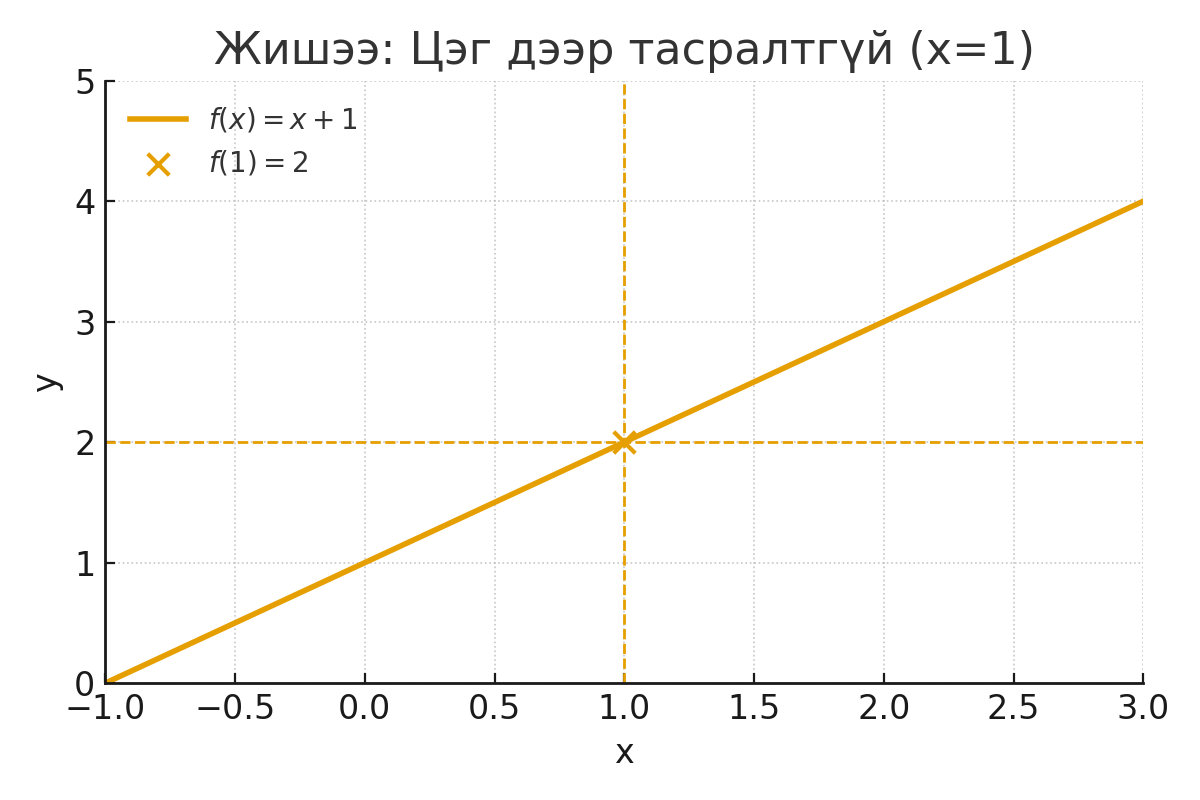
\includegraphics[width=.7\linewidth,max width=\linewidth,max height=.72\textheight]{continuous_at_point.png}
\end{center}
\end{example}
\end{frame}

\begin{frame}[allowframebreaks]{Тасралтгүй функц}
\begin{example}
\begin{remark}
Хэрэв 
$\displaystyle g(x)=\begin{cases}
\dfrac{x^2-1}{x-1}, & x\ne 1,\\
2, & x=1
\end{cases}$
тодорхойлбол $g(x)$ нь мөн $x=1$ дээр тасралтгүй болно, учир нь $g(x)=x+1$ байна.
\end{remark}
\end{example}
\end{frame}

\begin{frame}[allowframebreaks]{Тасралтгүй функц}
\begin{example}[Тасралтын жишээ]
\begin{enumerate}[label=\arabic*)]
\item $f(x)=\dfrac{1}{x^2}$ нь $(1,5)$ дээр тасралтгүй, харин $(-1,1)$ дээр $x=0$-д тодорхойлогдоогүй тул тасралттай.
\item $\displaystyle f(x)=\begin{cases}
\dfrac{x^2-3-\sqrt{x-1}}{x-2}, & x\ne 2,\\
3, & x=2
\end{cases}$ — $x=2$-д:
\begin{enumerate}[label=\alph*)]
\item $f(2)=3$.
\item $\displaystyle \lim_{x\to 2}\frac{x^2-3-\sqrt{x-1}}{x-2}
=\lim_{t\to 1}\frac{(t^2+1)^2-3-t}{t^2+1-2} = 3.5$ (орлуулалт $t=\sqrt{x-1}$).
\item $f(2)\ne \lim\limits_{x\to 2} f(x)$ тул тасралттай. (Хэрэв $f(2)=3.5$ бол тасралтгүй байна.)
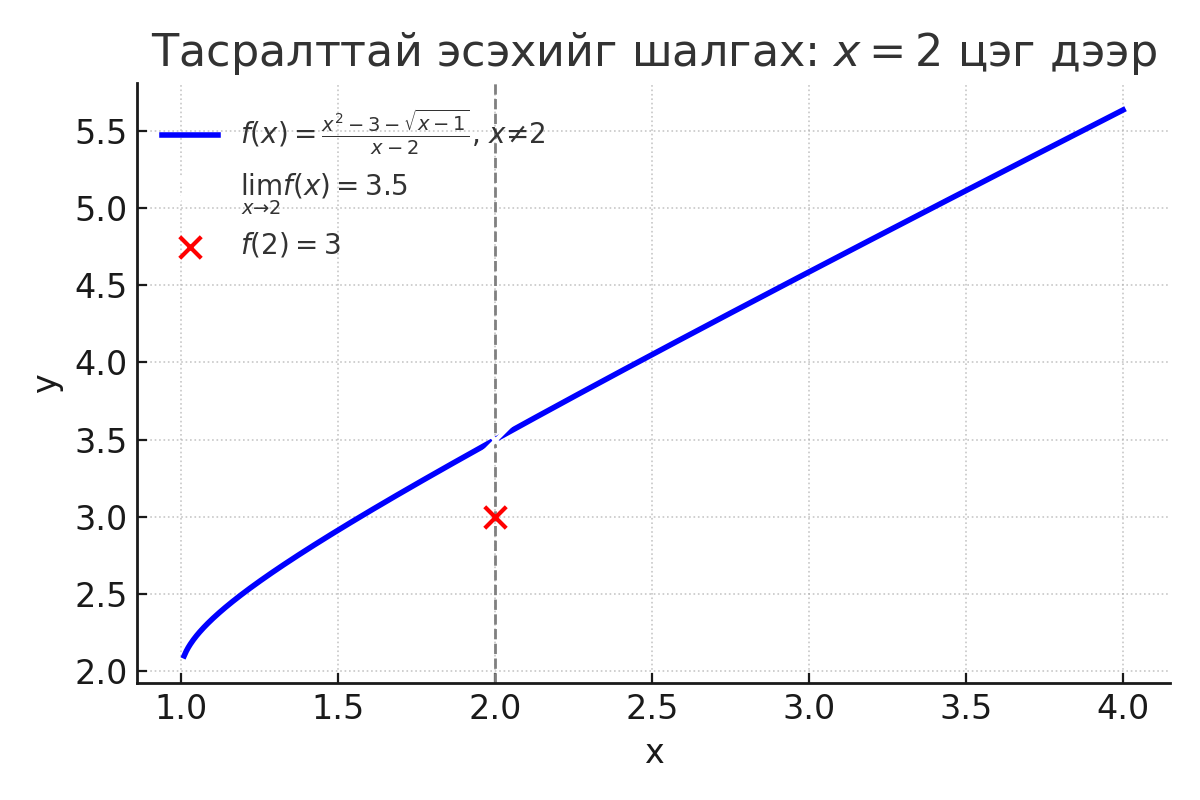
\includegraphics[scale=0.7,max width=\linewidth,max height=.72\textheight]{continuity_x2_case_white_dot.png}
\end{enumerate}
\end{enumerate}
\end{example}
\end{frame}

\begin{frame}[allowframebreaks]{Тасралтгүй функц}
\begin{theorem}[Арифметик үйлдлүүд] Хэрэв $f, g$ нь $x=a$-д тасралтгүй бол $f\pm g$, $f\cdot g$, мөн $g(a)\ne 0$ үед $\dfrac{f}{g}$ нь $x=a$-д тасралтгүй.
\end{theorem}
\end{frame}

\begin{frame}[allowframebreaks]{Тасралтгүй функц}
\begin{theorem}[Композици] Хэрэв $g$ нь $x=a$-д, $f$ нь $x=g(a)$-д тасралтгүй бол $f\circ g$ нь $x=a$-д тасралтгүй.
\end{theorem}
\end{frame}

\begin{frame}[allowframebreaks]{Тасралтгүй функц}
\begin{theorem}[Урвуу функц] Хэрэв $f$ урвуутай бөгөөд $x=a$-д тасралтгүй бол $f^{-1}$ нь $x=f(a)$-д тасралтгүй.
\end{theorem}
\end{frame}

\section{Өөрчлөлтийн харьцаа ба шүргэгч шулуун}
\begin{frame}[allowframebreaks]{Өөрчлөлтийн харьцаа ба шүргэгч шулуун}
\begin{definition}[Өөрчлөлтийн харьцаа]
$a,b$ нь $a\ne b$ тогтмол тоонууд байг. $y=f(x)$ функцийг $x=a$-аас $x=b$ хүртэл өөрчлөхөд
\[
\Delta x=b-a,\qquad \Delta y=f(b)-f(a),
\]
\[
\frac{\Delta y}{\Delta x}=\frac{f(b)-f(a)}{b-a}
\]
-ийг $f(x)$ функцийн $[a,b]$ дээрх өөрчлөлтийн харьцаа гэнэ. Энэ нь $A(a,f(a))$ ба $B(b,f(b))$ цэгүүдийг дайрсан \emph{хөвч} шулууны налалт юм.
\end{definition}
\end{frame}

\begin{frame}[allowframebreaks]{Өөрчлөлтийн харьцаа ба шүргэгч шулуун}
\begin{example}
$f(x)=x^2$ функцийн хувьд
\begin{enumerate}
  \item $x=-1$-ээс $x=2$ хүртэл: $\dfrac{\Delta y}{\Delta x}=\dfrac{2^2-(-1)^2}{2-(-1)}=\dfrac{3}{3}=1$.
  \item $x=a$-аас $x=a+h$ хүртэл: $\dfrac{(a+h)^2-a^2}{h}=2a+h$.
\end{enumerate}
\end{example}
\end{frame}

\section{Уламжлалын тодорхойлолт ба тэмдэглэгээ}
\begin{frame}[allowframebreaks]{Уламжлалын тодорхойлолт ба тэмдэглэгээ}
\begin{definition}[Цэг дээрх уламжлал]
$f$ функц $x=a$ цэгийн орчимд тодорхойлогдсон байг. Хэрэв
\[
\lim_{h\to 0}\frac{f(a+h)-f(a)}{h}
\]
хязгаар оршин байвал $f$ нь $x=a$ \textbf{цэг дээр дифференциалчлагдана} гэнэ; уг хязгаарыг $f'(a)$ буюу цэг дээрх уламжлал гэнэ.
\end{definition}
\end{frame}

\begin{frame}[allowframebreaks]{Уламжлалын тодорхойлолт ба тэмдэглэгээ}
\begin{note}
Цэг дээрх уламжлал $f'(a)$ нь $A(a,f(a))$ цэг дээр татсан шүргэгч шулууны налалт бөгөөд шүргэгчийн тэгшитгэл:
\[
y - f(a) = f'(a)\,(x-a).
\]
\end{note}
\end{frame}

\begin{frame}[allowframebreaks]{Уламжлалын тодорхойлолт ба тэмдэглэгээ}
\begin{example}
$f(x)=x^2-2x-1$ үед
\[
f'(3)=\lim_{h\to 0}\frac{f(3+h)-f(3)}{h}
=\lim_{h\to 0}\frac{(3+h)^2-2(3+h)-1 - (9-6-1)}{h}=4.
\]
\end{example}

\begin{center}
\begin{fitbox}\begin{tikzpicture}[scale=1]
  % Axes
  \draw[->] (-1,0) -- (5,0) node[right] {$x$};
  \draw[->] (0,-4) -- (0,6) node[above] {$y$};

  % f(x)=x^2-2x-1
  \draw[thick] plot[samples=200,domain=-0.2:4.5] (\x,{(\x*\x - 2*\x - 1)}) node[right] {$y=f(x)=x^2-2x-1$};

  % a=3 point
  \coordinate (P) at (3,{(3*3 - 2*3 - 1)});
  \fill (P) circle (2pt) node[above right] {$A(3,f(3))$};

  % tangent at x=3: f'(x)=2x-2 => f'(3)=4 ; y - f(3)=4(x-3)
  \draw[very thick,red] (1,{2+4*(1-3)}) -- (4.5,{2+4*(4.5-3)}) node[above right] {шүргэгч};

  % A few secants approaching tangent: pick b=3+h
  \foreach \h/\col in {1/blue,0.5/blue,0.25/blue}{
    \coordinate (B) at ({3+\h},{(3+\h)*(3+\h)-2*(3+\h)-1});
    \draw[\col] (P) -- (B);
    \fill (B) circle (1.5pt);
  }
\end{tikzpicture}\end{fitbox}
\end{center}
\end{frame}

\subsection*{Тэмдэглэгээ}
\begin{frame}[allowframebreaks]{Тэмдэглэгээ}
$y=f(x)$ бол $f'(x)$, $\dfrac{dy}{dx}$, $Df(x)$, $y'$ зэрэг тэмдэглэгээг хэрэглэнэ.
\end{frame}

% Семинар ба гэрийн даалгавар (Берманы бодлогын хураамжаас)
% Лекц 8: семинар ба гэрийн даалгавар. Бодлогууд: Г.Н. Берман, "Сборник задач по курсу
% математического анализа" (22-р хэвлэл). [Б.N] нь номын бодлогын дугаар.

\ProblemSet{Семинар 8}
\begin{frame}[allowframebreaks]{Семинар 8}
\pgroup{Тасралтгүй чанар ба тасралтын цэг.}
\begin{plist}
\prob{221}{$y=0$ \ ($x<0$), \ $y=x$ \ ($0\le x<1$), \ $y=-x^2+4x-2$ \ ($1\le x<3$), \ $y=4-x$ \ ($x\ge3$) функц тасралтгүй юу?}
\prob{223}{$f(x)=x+1$ \ ($x\le1$), \ $f(x)=3-ax^2$ \ ($x>1$). $a$-г ямар байхад $f$ тасралтгүй болох вэ? Графикийг байгуул.}
\prob{224}{$f(x)=-2\sin x$ \ ($x\le-\frac{\pi}{2}$), \ $A\sin x+B$ \ ($-\frac{\pi}{2}<x<\frac{\pi}{2}$), \ $\cos x$ \ ($x\ge\frac{\pi}{2}$). $f$ тасралтгүй байхаар $A,B$-г сонго.}
\prob{225}{$y=\frac{1}{x-2}$ ба $y=\frac{1}{(x+2)^2}$ функцүүд ямар цэгүүдэд тасрах вэ? Тасралтын цэгийн орчим дахь төлөвийн ялгааг тайлбарла.}
\prob{226}{$f(x)=\frac{x^2-1}{x^3-1}$ функц $x=1$ дээр тодорхойлогдоогүй. $x=1$ дээр тасралтгүй болгохын тулд $f(1)$ ямар байх ёстой вэ?}
\prob{227}{$y=\frac{\sin x}{x}$ ба $y=\frac{\cos x}{x}$ функцүүд $x=0$ дээр ямар төрлийн тасралттай вэ?}
\prob{228}{$y=\frac{|x|}{x}$ \ ($x\ne0$), \ $y=0$ \ ($x=0$) функцийн тасралтгүй чанарыг шинжилж, графикийг байгуул.}
\prob{230}{$y=\arctg\frac1x$ функцийг $x=0$ дээр тасралтгүй болгож дутуу тодорхойлж болох уу?}
\prob{232}{$f(x)=x\sin\frac{\pi}{x}$. Хаа сайгүй тасралтгүй байхын тулд $f(0)$ ямар байх ёстой вэ?}
\end{plist}
\pgroup{Уламжлалын тодорхойлолт.}
\begin{plist}
\prob{440}{$y=x^3$ функцийн $x_1=2$ цэг дээрх өөрчлөлтийг $\Delta x=2;\ 1;\ 0{,}5;\ 0{,}1$ үед ол.}
\prob{441.1}{$y=2x^3-x^2+1$, \ $x=1$, \ $\Delta x=0{,}1$ үед $\frac{\Delta y}{\Delta x}$-г олж, $\Delta x\to0$ үед хязгаар нь 4 болохыг харуул.}
\prob{443}{$f(x)=x^2$; \ $f'(5),\ f'(-2),\ f'\bigl(-\frac32\bigr)$-г тодорхойлолтоор ол.}
\prob{447}{$y=\sin x$ функцийн $x=0$ дээрх уламжлалыг тодорхойлолтоор ол.}
\prob{453}{Тэгш функцийн уламжлал сондгой, сондгой функцийн уламжлал тэгш функц болохыг батал.}
\prob{907}{$y=|x|$ функц $x=0$ дээр тасралтгүй боловч дифференциалчлагдахгүйг харуул.}
\end{plist}
\pgroup{Уламжлалын геометр утга.}
\begin{plist}
\prob{454}{$y=x^2$ параболын 1) координатын эх, 2) $(3;9)$, 3) $(-2;4)$ цэгүүд, 4) $y=3x-2$ шулуунтай огтлолцох цэгүүд дээрх шүргэгчийн өнцгийн коэффициентийг ол.}
\prob{456}{$y=x^2$ параболын ямар цэг дээрх шүргэгч 1) $Ox$ тэнхлэгтэй параллель, 2) $Ox$ тэнхлэгтэй $45^\circ$ өнцөг үүсгэх вэ?}
\prob{459}{$y=x^2$ ба $y^2=x$ параболууд ямар өнцгөөр огтлолцох вэ?}
\prob{461}{$y=x^3$ муруйн абсцисс нь 2 байх цэг дээрх шүргэгч ба нормалийн тэгшитгэлийг бич.}
\prob{463}{$y=x^2$ параболын ямар цэг дээрх шүргэгч 1) $y=4x-5$ шулуунтай параллель, 2) $2x-6y+5=0$ шулуунтай перпендикуляр, 3) $3x-y+1=0$ шулуунтай $45^\circ$ өнцөг үүсгэх вэ?}
\end{plist}
\end{frame}

\ProblemSet{Гэрийн даалгавар 8}
\begin{frame}[allowframebreaks]{Гэрийн даалгавар 8}
\pgroup{Тасралтгүй чанар ба тасралтын цэг.}
\begin{plist}
\prob{222}{Суурийн радиус нь 3, 2, 1 м, өндөр нь бүгд 5 м байх гурван цилиндрийг бие биен дээр нь тавив. Үүссэн биетийн хөндлөн огтлолын талбайг доод цилиндрийн доод суурь хүртэлх зайн функцээр илэрхийл. Энэ функц тасралтгүй юу? Графикийг байгуул.}
\prob{229}{$y=\frac{1}{\lg|x|}$ функц хэдэн тасралтын цэгтэй, ямар төрлийнх вэ? Графикийг байгуул.}
\prob{231}{$f(x)=\sin\frac{\pi}{2x}$ \ ($x\ne0$), \ $f(0)=1$ функцийн тасралтгүй чанарыг шинжил.}
\prob{233}{$y=\frac{1}{1+2^{1/x}}$ функц $x=0$ дээр I төрлийн тасралттайг батал.}
\prob{234}{$y=2^{-2^{1/(1-x)}}$ функцийн $x=1$ дээрх тасралтын төрлийг тогтоо. $x=1$ дээр тасралтгүй болгож тодорхойлж болох уу?}
\prob{235}{$y=\frac{2^{1/x}-1}{2^{1/x}+1}$ функцийн $x=0$ дээрх тасралтын төрлийг тогтоо.}
\prob{236}{$f(x)=(x+1)\,2^{-\left(\frac{1}{|x|}+\frac1x\right)}$ \ ($x\ne0$), \ $f(0)=0$. $[-2,2]$ дээр $f$ нь $f(-2)$ ба $f(2)$-ын хоорондох бүх утгыг авдаг боловч тасралттайг харуул (аль цэгт?).}
\prob{237}{$y=\frac{1}{1+2^{\tg x}}$ функцийн тасралтгүй чанарыг шинжил.}
\prob{238}{$x$ рационал бол $f(x)=0$, иррационал бол $f(x)=x$. $f$ ямар цэгт тасралтгүй вэ?}
\end{plist}
\pgroup{Уламжлалын тодорхойлолт.}
\begin{plist}
\prob{441.2}{$y=\frac1x$, \ $x=2$, \ $\Delta x=0{,}01$ үед $\frac{\Delta y}{\Delta x}$-г олж, $\Delta x\to0$ үед хязгаар нь $-\frac14$ болохыг харуул.}
\prob{442}{$y=x^2$ функцийн $x=3$ дээрх уламжлалын ойролцоо утгыг $\Delta x=0{,}5;\ 0{,}1;\ 0{,}01;\ 0{,}001$ үед ол.}
\prob{444}{$f(x)=x^3$; \ $f'(1),\ f'(0),\ f'(-\sqrt2),\ f'\bigl(\frac13\bigr)$-г ол.}
\prob{445}{$f(x)=x^2$. Ямар цэгт $f(x)=f'(x)$ байх вэ?}
\prob{446}{$f(x)=x^2$ функцийн хувьд $f'(a+b)=f'(a)+f'(b)$ биелэхийг шалга. $f(x)=x^3$-ийн хувьд биелэх үү?}
\prob{448}{$y=\lg x$ функцийн $x=1$ дээрх уламжлалыг ол.}
\prob{449}{$y=10^x$ функцийн $x=0$ дээрх уламжлалыг ол.}
\prob{450}{$f(0)=0$ ба $x\to0$ үед $\frac{f(x)}{x}$-ийн хязгаар оршин байдаг. Энэ хязгаар $f'(0)$-тэй тэнцүүг батал.}
\prob{451}{$f(0)=\varphi(0)=0$, $x=0$ дээр уламжлалтай, $\varphi'(0)\ne0$ бол $\displaystyle\lim_{x\to0}\frac{f(x)}{\varphi(x)}=\frac{f'(0)}{\varphi'(0)}$ болохыг батал.}
\prob{452}{$f(x)$ нь $x=a$ дээр уламжлалтай бол $\displaystyle\lim_{x\to a}\frac{xf(a)-af(x)}{x-a}=f(a)-af'(a)$ болохыг батал.}
\prob{908}{$y=|x^3|$ функцийн $x=0$ дээрх тасралтгүй ба дифференциалчлагдах чанарыг шинжил.}
\prob{909}{$f(x)=1+x$ \ ($x\le0$), \ $x$ \ ($0<x<1$), \ $2-x$ \ ($1\le x\le2$), \ $3x-x^2$ \ ($x>2$). $f$-ийн тасралтгүй чанарыг шинжилж, $f'(x)$ оршин байх ба тасралтгүй эсэхийг тогтоо.}
\end{plist}
\pgroup{Уламжлалын геометр ба физик утга.}
\begin{plist}
\prob{455}{$y=x^3$ кубын параболын ямар цэгүүдэд шүргэгчийн өнцгийн коэффициент 3-тай тэнцүү вэ?}
\prob{457}{$y=x^3$ кубын параболын шүргэгч $Ox$ тэнхлэгтэй мохоо өнцөг үүсгэж болох уу?}
\prob{458}{$y=x^2$ парабол ба $3x-y-2=0$ шулуун ямар өнцгөөр огтлолцох вэ?}
\prob{460}{$y=\frac1x$ гипербол ба $y=\sqrt x$ парабол ямар өнцгөөр огтлолцох вэ?}
\prob{462}{Аргументын ямар утгад $y=x^2$ ба $y=x^3$ муруйнуудын шүргэгчүүд параллель байх вэ?}
\prob{464}{$y=ax^2$ параболын дурын цэг дээрх дэд шүргэгч нь шүргэлтийн цэгийн абсциссын хагастай тэнцүүг батал. Үүнийг ашиглан шүргэгч байгуулах аргыг заа.}
\prob{432}{$AB$ нимгэн жигд бус саваа $L=20$ см урттай. $AM$ хэсгийн масс $M$ цэгээс $A$ хүртэлх зайн квадраттай пропорционал, $AM=2$ см хэсгийн масс 8 г. 1) $AM=2$ см хэсгийн дундаж нягт, 2) бүх савааны дундаж нягт, 3) $M$ цэг дэх нягтыг ол.}
\prob{433}{30 см урт $AB$ саваанд масс (граммаар) $m=3l^2+5l$ хуулиар тархсан ($l$ нь $A$-аас тоолсон урт). 1) Савааны дундаж шугаман нягт, 2) $l=5$ см цэг, $A$ цэг, савааны төгсгөл дэх нягтыг ол.}
\prob{434}{1 кг усыг $0$-ээс $t^\circ$C хүртэл халаах дулааны хэмжээ $Q=4186{,}8(t+0{,}00002t^2+0{,}0000003t^3)$ Ж. $t=30^\circ$ ба $t=100^\circ$ үеийн усны дулаан багтаамжийг ($Q'(t)$) ол.}
\end{plist}
\end{frame}


  % Лекц 9. Уламжлал
% Эх: latex/lectures/lec09-derivative-2.tex (scripts/latex_to_beamer.py-ээр хөрвүүлсэн)
% Frame бүр слайдад нэг (эсвэл allowframebreaks-аар хэд хэдэн) хуудас болно;
% хэвлэх хувилбарт frame-ийн хил харагдахгүй, текст үргэлжилсэн байна.

\MathLecture{9}{Уламжлал}

\section{Өөрчлөлтийн харьцаа ба шүргэгч шулуун}
\begin{frame}[allowframebreaks]{Өөрчлөлтийн харьцаа ба шүргэгч шулуун}
\begin{definition}[Өөрчлөлтийн харьцаа]
$a,b$ нь $a\ne b$ тогтмол тоонууд байг. $y=f(x)$ функцийг $x=a$-аас $x=b$ хүртэл өөрчлөхөд
\[
\Delta x=b-a,\qquad \Delta y=f(b)-f(a),
\]
\[
\frac{\Delta y}{\Delta x}=\frac{f(b)-f(a)}{b-a}
\]
-ийг $f(x)$ функцийн $[a,b]$ дээрх өөрчлөлтийн харьцаа гэнэ. Энэ нь $A(a,f(a))$ ба $B(b,f(b))$ цэгүүдийг дайрсан шулууны налалт юм.
\end{definition}
\end{frame}

\begin{frame}[allowframebreaks]{Өөрчлөлтийн харьцаа ба шүргэгч шулуун}
\begin{example}
$f(x)=x^2$ функцийн хувьд
\begin{enumerate}
  \item $x=-1$-ээс $x=2$ хүртэл: $\dfrac{\Delta y}{\Delta x}=\dfrac{2^2-(-1)^2}{2-(-1)}=\dfrac{3}{3}=1$.
  \item $x=a$-аас $x=a+h$ хүртэл: $\dfrac{(a+h)^2-a^2}{h}=2a+h$.
\end{enumerate}
\end{example}
\end{frame}

\section{Уламжлалын тодорхойлолт ба тэмдэглэгээ}
\begin{frame}[allowframebreaks]{Уламжлалын тодорхойлолт ба тэмдэглэгээ}
\begin{definition}[Цэг дээрх уламжлал]
$f$ функц $x=a$ цэгийн орчимд тодорхойлогдсон байг. Хэрэв
\[
\lim_{h\to 0}\frac{f(a+h)-f(a)}{h}
\]
хязгаар оршин байвал $f$ функцийг нь $x=a$ цэг дээр \textbf{цэг дээр дифференциалчлагдах} функц гэнэ. Энэ хязгаарын утгийг $f$ функцийн $a$ цэг дээрх уламжлал гээд $f'(a)$ гэж тэмдэглэнэ.
\end{definition}
\end{frame}

\begin{frame}[allowframebreaks]{Уламжлалын тодорхойлолт ба тэмдэглэгээ}
\begin{note}
$x=a$ цэг дээрх уламжлал $f'(a)$ нь $A(a,f(a))$ цэг дээр татсан шүргэгч шулууны налалт бөгөөд шүргэгч шулууны тэгшитгэл
\[
y - f(a) = f'(a)\,(x-a).
\] байдаг.
\end{note}
\end{frame}

\begin{frame}[allowframebreaks]{Уламжлалын тодорхойлолт ба тэмдэглэгээ}
\begin{example}
$f(x)=x^2-2x-1$ үед
\[
f'(3)=\lim_{h\to 0}\frac{f(3+h)-f(3)}{h}
=\lim_{h\to 0}\frac{(3+h)^2-2(3+h)-1 - (9-6-1)}{h}=4.
\]
\end{example}

\begin{center}
\begin{fitbox}\begin{tikzpicture}[scale=1]
  % Axes
  \draw[->] (-1,0) -- (5,0) node[right] {$x$};
  \draw[->] (0,-4) -- (0,6) node[above] {$y$};

  % f(x)=x^2-2x-1
  \draw[thick] plot[samples=200,domain=-0.2:4.5] (\x,{(\x*\x - 2*\x - 1)}) node[right] {$y=f(x)=x^2-2x-1$};

  % a=3 point
  \coordinate (P) at (3,{(3*3 - 2*3 - 1)});
  \fill (P) circle (2pt) node[above right] {$A(3,f(3))$};

  % tangent at x=3: f'(x)=2x-2 => f'(3)=4 ; y - f(3)=4(x-3)
  \draw[very thick,red] (1,{2+4*(1-3)}) -- (4.5,{2+4*(4.5-3)}) node[above right] {шүргэгч};

  % A few secants approaching tangent: pick b=3+h
  \foreach \h/\col in {1/blue,0.5/blue,0.25/blue}{
    \coordinate (B) at ({3+\h},{(3+\h)*(3+\h)-2*(3+\h)-1});
    \draw[\col] (P) -- (B);
    \fill (B) circle (1.5pt);
  }
\end{tikzpicture}\end{fitbox}
\end{center}
\end{frame}

\subsection*{Тэмдэглэгээ}
\begin{frame}[allowframebreaks]{Тэмдэглэгээ}
$y=f(x)$ бол түүний $a$ цэг дээрх уламжлалыг $f'(a)$, $\dfrac{dy}{dx}(a)$, $Df(a)$, $y'(a)$ зэрэг тэмдэглэнэ.
\end{frame}

\section{Хялбар функцүүдийн цэг дээрх уламжлал}
\begin{frame}[allowframebreaks]{Хялбар функцүүдийн цэг дээрх уламжлал}
\begin{example}
Дараах функцийг тодорхойлолтын дагуу бодож $x=a$ цэг дээрх уламжлалыг ол.
\begin{enumerate}
  \item $f(x)=c$ (тогтмол функц).  
  \[
  f'(a)=\lim_{h\to0}\frac{c-c}{h}=0.
  \]
  Тэгэхээр тогтмол функцийн цэг дээрх уламжлал $0$.
  
  \item $f(x)=x$.  
  \[
  f'(a)=\lim_{h\to0}\frac{(a+h)-a}{h}=\lim_{h\to0}1=1.
  \]
  Иймээс $y=x$ шулууны бүх цэг дээрх уламжлал $1$, өөрөөр хэлбэл шүргэгчийн налалт тогтмол.
  
  \item $f(x)=x^2$.  
  \[
  f'(a)=\lim_{h\to0}\frac{(a+h)^2-a^2}{h}=\lim_{h\to0}\frac{2ah+h^2}{h}=2a.
  \]
\end{enumerate}
\end{example}
\end{frame}

\section{Дифференциалчлах дүрмүүд}
\begin{frame}[allowframebreaks]{Дифференциалчлах дүрмүүд}
\begin{theorem}[Арифметик үйлдлүүд ба уламжлалын дүрмүүд]
$f,g$ дифференциалчлагддаг функцүүд ба  $c$ тогтмол тоо бол
\begin{enumerate}
    \item $(c\cdot f)'(a)=c\cdot f'(a)$
    \item $(f\pm g)'(a)=f'(a)\pm g'(a)$
    \item $(fg)'(a)=f'(a)g(a)+f(a)g'(a)$
    \item $
\left(\frac{f}{g}\right)'(a)=\frac{f'(a)g(a) - f(a)g'(a)}{g^2(a)}\quad (g(a)\ne 0)$
\end{enumerate}
байна.
\end{theorem}
\end{frame}

\begin{frame}[allowframebreaks]{Дифференциалчлах дүрмүүд}
\begin{example}
\begin{enumerate}
  \item $y=3x^2 \;\Rightarrow\; y'=6x$.
  \item $y=x^3+\tfrac12x^2-3x+4 \;\Rightarrow\; y'=3x^2+x-3$.
  \item $y=(x^2-1)(2x^2+x-3) \;\Rightarrow\; y'=8x^3+3x^2-10x-1$.
  \item $y=\dfrac{1}{x} \;\Rightarrow\; y'= -\dfrac{1}{x^{2}}$.
  \item $y=\dfrac{3x-2}{2x+1} \;\Rightarrow\; y'=\dfrac{7}{(2x+1)^2}$.
  \item $y=\sqrt{x}$. \textit{Бодолт:} $f(x)=\sqrt{x}$ гэж тавья. Тэгвэл
        $f(x)\cdot f(x)=x$. Уржвэрийн дүрмээр уламжлал авбал
        \[
           2\,f(x)\,f'(x) \;=\; 1
           \quad\Longrightarrow\quad
           f'(x) \;=\; \frac{1}{2\,f(x)} \;=\; \frac{1}{2\sqrt{x}}.
        \]
        Иймээс $y'=\dfrac{1}{2\sqrt{x}}$.
\end{enumerate}
\end{example}
\end{frame}

\begin{frame}[allowframebreaks]{Дифференциалчлах дүрмүүд}
\begin{definition}[Уламжлалын функц]
Хэрэв $f(x)$ функц нь тодорхойлогдох мужийнхаа \emph{бүх цэг дээр} уламжлалтай бол 
тэрхүү цэг $x$ бүрт $f'(x)$ тоог харгалзуулах функцийг $f$-ийн уламжлалын функц гэнэ.  

Өөрөөр хэлбэл, хэрэв $f$ нь муж $D$-ийн бүх цэг дээр уламжлалтай бол  
\[
g:D\to\mathbb{R}, \qquad g: x\to f'(x)
\]
функцийг $f$-ийн уламжлалын функц гэж нэрлээд $g(x)=f'(x)$ гэнэ.
\end{definition}
\end{frame}

\section{Тасралтгүй ба дифференциалчлагдах чанар}
\begin{frame}[allowframebreaks]{Тасралтгүй ба дифференциалчлагдах чанар}
\begin{theorem}
$f$ функц $x=a$ цэг дээр дифференциалчлагдвал $f$ нь $x=a$ цэг дээр тасралтгүй.
\end{theorem}

\begin{prof}
$h=x-a$ гэе. Тэгвэл
\[
\lim_{x\to a} \big(f(x)-f(a)\big)=\lim_{h\to 0}\frac{f(a+h)-f(a)}{h}\cdot h
= f'(a)\cdot 0=0.
\]
Иймээс $\displaystyle \lim_{x\to a}f(x)=f(a)$ буюу $f$ нь цэг дээр тасралтгүй.
\end{prof}
\end{frame}

\begin{frame}[allowframebreaks]{Тасралтгүй ба дифференциалчлагдах чанар}
\begin{example}[Тасралттай боловч дифференциалчлагдахгүй функц]
\begin{enumerate}
  \item $f(x)=|x|$ байг. $\displaystyle \lim_{h\to 0^+}\frac{|h|}{h}=1$, $\displaystyle \lim_{h\to 0^-}\frac{|h|}{h}=-1$ тул $x=0$ цэг дээрх уламжлал оршихгүй.
  \item $f(x)=\sqrt{|x|}$: $\displaystyle \lim_{h\to 0^+}\frac{\sqrt{|h|}}{h}=+\infty$, $\displaystyle \lim_{h\to 0^-}\frac{\sqrt{|h|}}{h}=-\infty$ — шүргэгч босоо.
\end{enumerate}
\end{example}

\begin{center}
\begin{fitbox}\begin{tikzpicture}[scale=1.0]
  % Axes
  \draw[->] (-3,0) -- (3,0) node[right] {$x$};
  \draw[->] (0,-0.5) -- (0,3.2) node[above] {$y$};

  % |x|
  \draw[thick] plot[samples=200,domain=-2.5:2.5] (\x,{abs(\x)}) node[right] {$y=|x|$};
  % One-sided slopes annotation
  \draw[red,very thick] (-2,-2) -- (0,0);
  \draw[red,very thick] (0,0) -- (2,2);
  \fill (0,0) circle (2pt) node[below left] {$x=0$};

  \node[below] at (-1.2,-0.2) {налалт $-1$};
  \node[above] at (1.2,1.4) {налалт $+1$};
\end{tikzpicture}\end{fitbox}
\hspace{1cm}
\begin{fitbox}\begin{tikzpicture}[scale=1.0]
  % Axes
  \draw[->] (-3,0) -- (3,0) node[right] {$x$};
  \draw[->] (0,-0.5) -- (0,2.8) node[above] {$y$};

  % sqrt(|x|)
  \draw[thick,domain=0:2.8,samples=200] plot (\x,{sqrt(\x)}) node[right] {$y=\sqrt{|x|}$};
  \draw[thick,domain=-2.8:0,samples=200] plot (\x,{sqrt(abs(\x))});

  % Vertical tangent indication
  \draw[red,very thick] (0,0) -- (0,2.2) node[above] {босоо шүргэгч};
  \fill (0,0) circle (2pt) node[below left] {$x=0$};
\end{tikzpicture}\end{fitbox}
\end{center}
\end{frame}

\section{Тригонометр, илтгэгч ба логарифм функцийн уламжлал}
\begin{frame}[allowframebreaks]{Тригонометр, илтгэгч ба логарифм функцийн уламжлал}
\begin{theorem}[Тригонометр функцийн уламжлал]
\[
(\sin x)' = \cos x, \qquad (\cos x)' = -\sin x
\]
\end{theorem}
\begin{prof}
\begin{enumerate}
  \item  
  Тодорхойлолтоор:
  \[
  \lim_{h\to0}\frac{\sin(x+h)-\sin x}{h}
  =\lim_{h\to0}\frac{\sin x\cos h+\cos x\sin h-\sin x}{h}
  =\lim_{h\to0}\big(\sin x\frac{\cos h-1}{h}+\cos x\frac{\sin h}{h}\big).
  \]
  $\displaystyle \lim_{h\to0}\frac{\cos h-1}{h}=0$ ба $\displaystyle \lim_{h\to0}\frac{\sin h}{h}=1$ тул:
  \[
  (\sin x)'=\cos x.
  \]

  \item $(\cos x)'=-\sin x$.  
  $$
  \lim_{h\to0}\frac{\cos(x+h)-\cos x}{h}
  =\lim_{h\to0}\frac{\cos x\cos h-\sin x\sin h-\cos x}{h}
  =$$
  $$\lim_{h\to0}\big(\cos x\frac{\cos h-1}{h}-\sin x\frac{\sin h}{h}\big)
  =-\sin x.
  $$
\end{enumerate}
\end{prof}
\end{frame}

\begin{frame}[allowframebreaks]{Тригонометр, илтгэгч ба логарифм функцийн уламжлал}
\begin{example}
\begin{enumerate}
  \item $y=\sin 2x \;\Rightarrow\; y'=(2\sin x\cos x)'=2(\cos x\cos x+\sin x(-\sin x))=2\cos 2x.$
  \item $y=\tan x=\dfrac{\sin x}{\cos x} 
  \;\Rightarrow\; y'=\dfrac{\cos^2 x+\sin^2 x}{\cos^2 x}
  =\dfrac{1}{\cos^2 x}.$
\end{enumerate}
\end{example}

\begin{center}
\begin{fitbox}\begin{tikzpicture}[scale=1]
  \draw[->] (-0.5,0) -- (7,0) node[right] {$x$};
  \draw[->] (0,-1.5) -- (0,1.5) node[above] {$y$};
  \draw[thick,domain=0:6.3,samples=200] plot(\x,{sin(\x r)}) node[right] {$y=\sin x$};
  \draw[red,thick,domain=0:6.3,samples=200] plot(\x,{cos(\x r)}) node[right] {$y'=\cos x$};
  \node[below right] at (1.57,0) {$\frac{\pi}{2}$};
  \node[below right] at (3.14,0) {$\pi$};
  \node[below right] at (4.71,0) {$\frac{3\pi}{2}$};
\end{tikzpicture}\end{fitbox}
\end{center}
\end{frame}

\section{Илтгэгч ба урвуу функцийн уламжлал}
\subsection*{Илтгэгч функцийн уламжлал ба хэрэглээ}
\begin{frame}[allowframebreaks]{Илтгэгч функцийн уламжлал ба хэрэглээ}
\begin{theorem}[Илтгэгч функцийн уламжлал]
\[
(e^x)' = e^x.
\]
\end{theorem}

\begin{prof}
Тодорхойлолтоор:
\[
(e^x)' = \lim_{h\to 0} \frac{e^{x+h} - e^x}{h}
= e^x \lim_{h\to 0}\frac{e^h - 1}{h}.
\]
Хязгаар $\displaystyle \lim_{h\to 0}\frac{e^h - 1}{h}=1$ тул $(e^x)'=e^x$.
\end{prof}
\end{frame}

\begin{frame}[allowframebreaks]{Илтгэгч функцийн уламжлал ба хэрэглээ}
\begin{example}
\begin{enumerate}
  \item $y=e^{2x}$ бол :
  \[
  y' = (e^{2x})'=(e^x\cdot e^x)'=e^x\cdot e^x+e^x\cdot e^x = 2e^{2x}.
  \]
  \item $y=e^{-x}$ бол
  \[
  y' = (e^{-x})'=\left(\dfrac{1}{e^x}\right)'=\dfrac{1'\cdot e^x-1\cdot (e^x)'}{(e^x)^2}= -e^{-x}.
  \]
\end{enumerate}
\end{example}
\end{frame}

\begin{frame}[allowframebreaks]{Илтгэгч функцийн уламжлал ба хэрэглээ}
\begin{theorem}[Давхар функцийн уламжлал]
Хэрэв $y=g(x)$ функц нь $x=a$ цэг дээр дифференциалчлагддаг, $y=f(x)$ нь $x=g(a)$ цэг дээр дифференциалчлагддаг бол $y=f(g(x))$ функц $x=a$ цэг дээр дифференциалчлагдах ба
\[
\boxed{\frac{dy}{dx}(a) = \frac{dy}{du}(a)\cdot\frac{du}{dx}(a)}.
\] байна.
\end{theorem}
\end{frame}

\begin{frame}[allowframebreaks]{Илтгэгч функцийн уламжлал ба хэрэглээ}
\begin{example}
\begin{enumerate}
  \item $y=a^x=e^{x\ln a}$ тул $(a>0, a\ne1)$ үед:
  \[
  y' = e^{x\ln a}\cdot \ln a = a^x \ln a.
  \]
  \item $y=\sin(e^x)$:
  \[
  y' = \cos(e^x)\cdot e^x.
  \]
  \item $y=e^{\sin x}$:
  \[
  y' = e^{\sin x}\cdot \cos x.
  \]
  \item $y=\sqrt{1+e^{2x}}$:
  \[
  y'=\frac{1}{2\sqrt{1+e^{2x}}}\cdot 2e^{2x}\cdot 1
  =\frac{e^{2x}}{\sqrt{1+e^{2x}}}.
  \]
\end{enumerate}
\end{example}
\end{frame}

\begin{frame}[allowframebreaks]{Илтгэгч функцийн уламжлал ба хэрэглээ}
\begin{theorem}[Урвуу функцийн уламжлалын теорем]
Урвуутай функц $y=f(x)$ нь $x=a$ цэг дээр уламжлалттай, $f(a)=b$ утгатай, $f'(a)\neq0$ гэж бодъё. Тэгвэл $y=f(x)$-ийн урвуу функц $y=f^{-1}(x)$ нь $x=b$ цэг дээр дифференциалчлагдах ба 
\[
\boxed{(f^{-1})'(b) = \dfrac{1}{f'(a)}=\dfrac{1}{f'(f^{-1}(b))}}
\] байна.
\end{theorem}
\end{frame}

\begin{frame}[allowframebreaks]{Илтгэгч функцийн уламжлал ба хэрэглээ}
\begin{example}
\begin{enumerate}
  \item $y=\ln x$ бол $x=e^y$. Урвуу функцийн дүрмээр:
  \[
  \frac{dy}{dx} = \frac{1}{\frac{dx}{dy}} = \frac{1}{e^y} = \frac{1}{x}.
  \]
  \item $y=\arcsin x$ бол $\sin y = x$. Дифференциал авбал:
  \[
  \cos y \, \frac{dy}{dx} = 1
  \quad \Longrightarrow \quad
  \frac{dy}{dx} = \frac{1}{\cos y}.
  \]
  Харин $\cos y = \sqrt{1-\sin^2 y}=\sqrt{1-x^2}$ тул:
  \[
  (\arcsin x)' = \frac{1}{\sqrt{1-x^2}}.
  \]
  \item $y=\arctan x$: $\tan y = x$ тул $\sec^2 y\,\dfrac{dy}{dx}=1$ буюу
  \[
  (\arctan x)'=\cos^2 y=\frac{1}{1+\tan^2 y}=\frac{1}{1+x^2}.
  \]
\end{enumerate}
\end{example}
\end{frame}

\section{Уламжлал бодох техник}
\subsection*{1. Уламжлалын жагсаалт}
\begin{frame}[allowframebreaks]{1. Уламжлалын жагсаалт}
\begin{enumerate}
  \item $(c)'=0$ — тогтмол функцийн уламжлал $0$.
  \item $(x)'=1$ , $y=x$ функцийн уламжлал $1$.
  \item $(x^{a})'=ax^{a-1}$ \;($a\in\mathbb{R}$).
  \item $(e^x)'=e^x$, \; $(a^x)'=a^x\ln a$.
  \item $(\ln x)'=\dfrac{1}{x}$.
  \item $(\sin x)'=\cos x$, \; $(\cos x)'=-\sin x$, \; $(\tan x)'=\dfrac{1}{\cos^2 x}$.
  \item $(cf)'=cf'$, \; $(f\pm g)'=f'\pm g'$, \; $(fg)'=f'g+fg'$, \;
  $\displaystyle \left(\dfrac{f}{g}\right)'=\dfrac{f'g-fg'}{g^2}$.
  \item \textbf{Гинжин дүрэм:} $(f(g(x)))'=f'(g(x))\cdot g'(x)$.
\end{enumerate}
\end{frame}

\subsection*{2. Бодлого бодох жор}
\begin{frame}[allowframebreaks]{2. Бодлого бодох жор}
\begin{itemize}
  \item \textbf{Эхлээд} логgарифм, илтгэгч, зэрэг, тригнометр—аль дүрэм хэрэглэхийг тодорхойл.
  \item \textbf{Дараа нь} үржвэр/ногдвор/гинжин аль нь давамгайлж буйг тогтоож, \textbf{давхар} хэрэглэж эвлүүл.
  \item \textbf{Хялбарчлах хувиргалт} (триг $=\dfrac{\sin}{\cos}$, $\ln\sqrt{\ }=\tfrac12\ln$ гэх мэт) хийж хялбарчил.
\end{itemize}
\end{frame}

\subsection*{3. Хялбар жишээнүүд}
\begin{frame}[allowframebreaks]{3. Хялбар жишээнүүд}
\begin{example}
\begin{enumerate}
  \item $y=\dfrac{\sin x}{x}$.\; $y'=\dfrac{x\cos x-\sin x}{x^2}$.
  \item $y=e^{2x-3}$.\; $y'=2e^{2x-3}$.
  \item $y=\ln(\sqrt{1+x^2})$.\; $y'=\dfrac{x}{1+x^2}$ \; (гинжин + $\ln\sqrt{\ }=\tfrac12\ln$).
  \item $y=\sin(e^x)$.\; $y'=\cos(e^x)\cdot e^x$.
  \item $y=(x^2+1)^{5}$.\; $y'=5(x^2+1)^{4}\cdot 2x=10x(x^2+1)^4$.
\end{enumerate}
\end{example}
\end{frame}

\subsection*{4.Далд функцийн уламжлал}
\begin{frame}[allowframebreaks]{4.Далд функцийн уламжлал}
\begin{definition}
$F(x,y)=0$ тэгшитгэлийнхэлбэрийн хамаарлыг $y=y(x)$ гэж үзээд $x$-ийн хувьд дифференциалчлахыг \emph{имплицит уламжлал} гэнэ.
\end{definition}
\end{frame}

\begin{frame}[allowframebreaks]{4.Далд функцийн уламжлал}
\begin{example}
Тойрог: $x^2+y^2=25$. $x$-ийн хувьд дифференциалчилбал $2x+2y\,y'=0 \Rightarrow y'=-\dfrac{x}{y}$.
\end{example}
\end{frame}

\begin{frame}[allowframebreaks]{4.Далд функцийн уламжлал}
\begin{example}
$xy+\sin y = x^2$. Дифференциалчилбал
\[
y + x\,y' + \cos y \cdot y' = 2x 
\;\;\Rightarrow\;\;
y'(x+\cos y)=2x-y
\;\;\Rightarrow\;\;
\boxed{y'=\dfrac{2x-y}{\,x+\cos y\,}}.
\]
\end{example}
\end{frame}

\subsection*{5. Логарифмын уламжлал (Зэрэгт-илтгэгч функц)}
\begin{frame}[allowframebreaks]{5. Логарифмын уламжлал (Зэрэгт-илтгэгч функц)}
\begin{remark}
$y>0$ үед $\ln y$ авч, тэгшитгэлийг логарифмдан хоёр талд нь дифференциалчлах аргыг \emph{логарифмын уламжлал} гэдэг.
\end{remark}
\end{frame}

\begin{frame}[allowframebreaks]{5. Логарифмын уламжлал (Зэрэгт-илтгэгч функц)}
\begin{example}
$y=x^x$ ($x>0$). $\ln y = x\ln x \Rightarrow \dfrac{y'}{y}=\ln x + 1 \Rightarrow \boxed{y'=x^x(\ln x + 1)}$.
\end{example}
\end{frame}

\begin{frame}[allowframebreaks]{5. Логарифмын уламжлал (Зэрэгт-илтгэгч функц)}
\begin{example}
$y=(x^2+1)^x$ ($x>0$). $\ln y = x\ln(x^2+1)\Rightarrow \dfrac{y'}{y}=\ln(x^2+1)+\dfrac{2x^2}{x^2+1}$.\\
Иймд $\boxed{y'=(x^2+1)^x\!\left[\ln(x^2+1)+\dfrac{2x^2}{x^2+1}\right]}$.
\end{example}
\end{frame}

\subsection*{6. $\boldsymbol{a^x}$ ба $\boldsymbol{\log}$–ын \emph{хэрэглээ}}
\begin{frame}[allowframebreaks]{6. $\boldsymbol{a^x}$ ба $\boldsymbol{\log}$–ын \emph{хэрэглээ}}
\begin{example}
\begin{enumerate}
  \item $y=a^x$ ($a>0,a\ne1$). $y'=a^x\ln a$. \;
        Ж: $y=2^{3x}$ бол $y'=3\ln2\cdot 2^{3x}$.
  \item $y=\dfrac{\ln x}{x^2}$.\; $y'=\dfrac{1}{x}\cdot\dfrac{1}{x^2} + \ln x \cdot \left(-\dfrac{2}{x^3}\right)=\dfrac{1-2\ln x}{x^3}$.
  \item $y=e^{\sqrt{x}}$.\; $y'=e^{\sqrt{x}}\cdot\dfrac{1}{2\sqrt{x}}$.
  \item $y=\log_a(\sqrt{x})$.\; $y'=\dfrac{1}{x\ln a}\cdot\dfrac{1}{2}=\dfrac{1}{2x\ln a}$.
\end{enumerate}
\end{example}
\end{frame}

% Семинар ба гэрийн даалгавар (Берманы бодлогын хураамжаас)
% Лекц 9: семинар ба гэрийн даалгавар. Бодлогууд: Г.Н. Берман, "Сборник задач по курсу
% математического анализа" (22-р хэвлэл). [Б.N] нь номын бодлогын дугаар.

\ProblemSet{Семинар 9}
\begin{frame}[allowframebreaks]{Семинар 9}
\pgroup{Зэрэгт ба рационал функцийн уламжлалыг ол.}
\begin{plist}
\prob{466.8}{$y=\frac{mx^2}{\sqrt x}+\frac{nx\sqrt x}{\sqrt[3]{x}}-\frac{p\sqrt x}{x}$}
\prob{471.7}{$y=(1+\sqrt x)(1+\sqrt{2x})(1+\sqrt{3x})$}
\prob{476}{$y=\frac{ax+b}{cx+d}$}
\prob{479}{$y=\frac{1-x^3}{1+x^3}$}
\prob{491}{$F(x)=(x-1)(x-2)(x-3)$; \ $F'(0),\ F'(1),\ F'(2)$-г ол.}
\end{plist}
\pgroup{Давхар функцийн уламжлалыг ол.}
\begin{plist}
\prob{498.8}{$y=\bigl(7x^2-\frac4x+6\bigr)^6$}
\prob{501}{$y=\frac{1+\sqrt x}{1+\sqrt{2x}}$}
\prob{508}{$y=\sqrt[3]{\frac{1}{1+x^2}}$}
\prob{515}{$y(x)=\sqrt{\frac{x+1}{x-1}}$; \ $y'(2)$-г ол.}
\end{plist}
\pgroup{Тригонометр ба урвуу тригонометр функц.}
\begin{plist}
\prob{523}{$y=\frac{x}{\sin x+\cos x}$}
\prob{536}{$y=\sqrt{1+2\tg x}$}
\prob{541}{$y=\sin\sqrt{1+x^2}$}
\prob{551}{$y=x\arcsin x+\sqrt{1-x^2}$}
\prob{562}{$y=\arccos\frac{2x-1}{\sqrt3}$}
\end{plist}
\pgroup{Логарифм ба илтгэгч функц.}
\begin{plist}
\prob{586}{$y=\ln(x^2-4x)$}
\prob{589}{$y=\ln\tg x$}
\prob{612}{$y=(x^2-2x+3)e^x$}
\prob{623}{$y=e^{\arcsin2x}$}
\end{plist}
\pgroup{Логарифмчлэн уламжлалыг ол.}
\begin{plist}
\prob{650}{$y=x^{x^2}$}
\prob{652}{$y=(\sin x)^{\cos x}$}
\end{plist}
\end{frame}

\ProblemSet{Гэрийн даалгавар 9}
\begin{frame}[allowframebreaks]{Гэрийн даалгавар 9}
\pgroup{Зэрэгт ба рационал функцийн уламжлалыг ол.}
\begin{plist}
\prob{466.10}{$y=0{,}1t^{-2/3}-\frac{5{,}2}{t^{1{,}4}}+\frac{2{,}5}{\sqrt[5]{t}}$}
\prob{471.5}{$y=(\sqrt[3]{x}+2x)(1+\sqrt[3]{x^2}+3x)$}
\prob{473}{$y=\frac{x}{x^2+1}$}
\prob{486}{$y=\frac{x^2+x-1}{x^3+1}$}
\prob{489}{$y=\frac{a^2b^2c^2}{(x-a)(x-b)(x-c)}$}
\prob{470}{$f(x)=4-5x+2x^3-x^5$. \ $f'(a)=f'(-a)$ болохыг харуул.}
\end{plist}
\pgroup{Давхар функцийн уламжлалыг ол.}
\begin{plist}
\prob{498.11}{$y=\bigl(\frac{1+x^2}{1+x}\bigr)^5$}
\prob{500}{$s=\frac{t^3}{(1-t)^2}$}
\prob{507}{$y=\frac{1}{\sqrt{a^2-x^2}}$}
\prob{510}{$y=\frac{1+x}{\sqrt{1-x}}$}
\prob{513}{$y=\frac{1}{\sqrt[3]{2x-1}}+\frac{5}{\sqrt[4]{(x^2+2)^3}}$}
\prob{516}{$y(x)=\sqrt{\frac{1-x^2}{1+x^2}}$; \ $y'(0)$-г ол.}
\end{plist}
\pgroup{Тригонометр ба урвуу тригонометр функц.}
\begin{plist}
\prob{524}{$y=\frac{x\sin x}{1+\tg x}$}
\prob{529}{$y=\frac13\tg^3x-\tg x+x$}
\prob{539}{$y=\cos^34x$}
\prob{545}{$y=\cos^2\frac{1-\sqrt x}{1+\sqrt x}$}
\prob{558}{$y=\frac{x}{1+x^2}-\arctg x$}
\prob{567}{$y=\sqrt{1-(\arccos x)^2}$}
\prob{568}{$y=\arcsin\sqrt{\frac{1-x}{1+x}}$}
\prob{572}{$y=\arctg\bigl(x-\sqrt{1+x^2}\bigr)$}
\end{plist}
\pgroup{Логарифм ба илтгэгч функц.}
\begin{plist}
\prob{581}{$y=\frac{1-\ln x}{1+\ln x}$}
\prob{590}{$y=\ln\arccos2x$}
\prob{595}{$y=\ln\arctg\sqrt{1+x^2}$}
\prob{613}{$y=\frac{1+e^x}{1-e^x}$}
\prob{616}{$y=xe^x(\cos x+\sin x)$}
\prob{626}{$y=\sin\bigl(e^{x^2+3x-2}\bigr)$}
\end{plist}
\pgroup{Логарифмчлэн уламжлалыг ол.}
\begin{plist}
\prob{653}{$y=(\ln x)^x$}
\prob{656}{$y=\frac{(x-2)^2\sqrt[3]{x+1}}{(x-5)^3}$}
\prob{661}{$y=x^{1/x}$}
\prob{665}{$y=(x^2+1)^{\sin x}$}
\end{plist}
\end{frame}

% Лекц 10. Параметр ба далд функцийн уламжлал, дээд эрэмбийн уламжлал
% Эх: latex/lectures/lec10-derivative-3.tex (scripts/latex_to_beamer.py-ээр хөрвүүлсэн)
% Frame бүр слайдад нэг (эсвэл allowframebreaks-аар хэд хэдэн) хуудас болно;
% хэвлэх хувилбарт frame-ийн хил харагдахгүй, текст үргэлжилсэн байна.

\MathLecture{10}{Параметр ба далд функцийн уламжлал, дээд эрэмбийн уламжлал}

\section{Параметр ба далд функцийн уламжлал}
\begin{frame}[allowframebreaks]{Параметр ба далд функцийн уламжлал}
\begin{definition}[Параметр функц]
 $g(t),\ h(t)$ функцүүд өгөгдсөн ба $t\in(\alpha;\beta)$ үед $g(t)$ функц иньектив  байг.
 
 $D=\{g(t)|t\in(\alpha;\beta)\}$-г  $E=\{h(t)|t\in(\alpha;\beta)\}$ олонлогт буулгасан функцийг 
 $$f: g(t)\to h(t)$$ дүрмээр тодорхойлож болно. Энэ функцийг параметр функц гээд 
 $$ f:
 \begin{cases}
     x=g(t)\\
     y=h(t)
 \end{cases}$$ гэж тэмдэглэнэ. 
\end{definition}
Цаашид $y=f(x)$ хэлбэртэй өгөгдсөн функцийг ил хэлбэртэй гэж нэрлэе. Ил функцийг $$ f:
 \begin{cases}
     x=t\\
     y=f(t)
 \end{cases}$$ гэж параметр хэлбэрээр бичиж болно. Тодорхойлолт ёсоор $g(t)$ функц иньектив учир $$g: (\alpha;\beta)\to D$$ буулгалт биектив байна. Тиймээс $g^{-1}: D\to (\alpha;\beta)$ буулгалт оршин байна. Иймд 
 $$y=h(t)=h(g^{-1}(x))\qquad x\in D$$ байдлаар далд функцийг ил байдлаар илэрхийлж болно.
\end{frame}

\begin{frame}[allowframebreaks]{Параметр ба далд функцийн уламжлал}
 \begin{example}
$x(t)=t+1,\quad y(t)=t^3-3t$ байг. Энэ функцийн хувьд $t=1$ үед $f:2\to -2$, $t=-2$ үед $f:-1\to 2$ байна. $t=x-1$ тул 
\[y=t^3-3t=(x-1)^3-3(x-1)=x^3-3x^2+2
\] гэж ил хэлбэрээр бичиж болно.
\end{example}
\end{frame}

\begin{frame}[allowframebreaks]{Параметр ба далд функцийн уламжлал}
\begin{theorem}[Параметр функцийн уламжлал] 
$$ f:
 \begin{cases}
     x=g(t)\\
     y=h(t)
 \end{cases}$$ функцийн хувьд 
$g(z)=a, g'(z), h'(z)$ оршин байдаг $g'(z)\neq 0$ бол 
\[
f'(a)=\frac{dy}{dx}(a)=\frac{dh/dt}{dg/dt}=\frac{h'(z)}{g'(z)}
\] байна.
Өөрөөр хэлбэл 
$$ f':
 \begin{cases}
     x=g(t)\\
     y'=\frac{h'(t)}{g'(t)}
 \end{cases}$$ гэсэн параметр функц байна.
\end{theorem}

\begin{prof} $$y=h(t)=h(g^{-1}(x))\qquad x\in D$$ байдлаар далд функцийг ил байдлаар илэрхийлж болох тул гинжин дүрэм ба урвуу функцийн уламжлалын тухай теорем хэрэглэвэл 
$$\dfrac{dy}{dx}(a)=\dfrac{dh}{dt}(z)\cdot \dfrac{dg^{-1}}{dt}(a)=\dfrac{h'(z)}{g'(z)}$$ болж батлагав.
\end{prof}
\end{frame}

\begin{frame}[allowframebreaks]{Параметр ба далд функцийн уламжлал}
\begin{example}
$x(t)=t^2+1,\quad y(t)=t^3-3t ,\quad t\geq 0$ байг. 
\[
x'(t)=2t,\qquad y'(t)=3t^2-3,\qquad
\frac{dy}{dx}=\frac{3t^2-3}{2t}.
\] Өөрөөр хэлбэл $t=1$ үед $x=2, y=-2$ ба энэ цэг дээрх уламжлал $y'(2)=0$ байна.  
\end{example}
\end{frame}

\begin{frame}[allowframebreaks]{Параметр ба далд функцийн уламжлал}
\begin{example}
Нэгж тойрог: $x(t)=\cos t,\ y(t)=\sin t \quad t\in [0;\pi]$ байг.
\[
x'=-\sin t,\quad y'=\cos t,\quad
\frac{dy}{dx}=\frac{\cos t}{-\sin t}=-\cot t.
\]
$t=\frac{\pi}{2}$ дээр $x=0, y=1$ тул $\frac{dy}{dx}=0$ хэвтээ шүргэгчтэй ба $t=0$ дээр $x=1,y=0$ тул $\dfrac{dy}{dx}=-\infty$ тул босоо шүргэгч шулуунтай.
\end{example}
\end{frame}

\begin{frame}[allowframebreaks]{Параметр ба далд функцийн уламжлал}
\begin{definition}[Далд функц]  $(a,b)$ хос нь 
$F(z,u)=0$ тэгшитгэлийг хангадаг ба $\forall x\in (a-\delta;a+\delta)$ хувьд $F(x,u)=0$ тэгшитгэл $u=y\in E\subset\mathbf{R}$ байх ганц шийдтэй байг. Энд $\delta>0$ тоо. Тэгвэл  $\forall x\in (a-\delta;a+\delta)$ бол $(a-\delta;a+\delta)$-г $E$ олонлогт буулгах функцийг $$f: x\to y$$ дүрмээр үүсгэж болох ба энэ функцийг $F(x,y)=0$ далд тэгшитгэлээр өгсөн функц гэнэ. Иймд $$F(x,y)=F(x,f(x))=0$$ байна. 
\end{definition}
\end{frame}

\begin{frame}[allowframebreaks]{Параметр ба далд функцийн уламжлал}
\begin{example}
$F(x,y)=x^2+y^2-1=0$ , $E=[0;1]$ байг. $x\in (-1;1)$ бол $y=\sqrt{1-x^2}$ байх $(x,y)$ хос нь $x^2+y^2-1=0$  тэгшитгэлийг хангана. Иймд далд функц тодорхойлож байна. Энэ нь $y(x)=\sqrt{1-x^2}$ ил функцтэй тэнцүү. Хэрэв $E=[-1;0]$ байсан бол $F(x,y)=x^2+y^2-1=0$ далд функц $y(x)=-\sqrt{1-x^2}$ ил функцийг тодорхойлно.
\end{example}
\end{frame}

\begin{frame}[allowframebreaks]{Параметр ба далд функцийн уламжлал}
\begin{theorem}[Далд функцийн уламжлал]
$F(x,y)=F(x,f(x))=0$ далд функцийн хувьд $f(a)=b$ бол $F_y(a,b)\neq 0$ үед $f'(a)$ оршин байх ба 
$$f'(a)=-\dfrac{F_x(a,b)}{F_y(a,b)}$$ байна. Энд $F_x$ нь $F(x,y)$ -с $y$ тогтмол гэж үзээд  $x$-р авсан уламжлал, $F_y$ нь $F(x,y)$ -с $x$ тогтмол гэж үзээд  $y$-р авсан уламжлал.
\end{theorem}
\end{frame}

\begin{frame}[allowframebreaks]{Параметр ба далд функцийн уламжлал}
\begin{example}
Тойргийн тэнцэтгэл:
\[
F(x,y)=x^2+y^2-1=0.
\]
$F_x = 2x, \; F_y = 2y$.  
Иймд:
\[
\frac{dy}{dx}=-\frac{F_x}{F_y}=-\frac{x}{y}.
\]
$(0,1)$ дээр $y'=0$ (хэвтээ шүргэгч), $(1,0)$ дээр $y'\to\infty$ (босоо шүргэгч).
\end{example}
\end{frame}

\begin{frame}[allowframebreaks]{Параметр ба далд функцийн уламжлал}
\begin{remark}
Далд функцийн уламжлал олох:
\begin{enumerate}
  \item Тэнцэтгэлийн хоёр талыг $x$-ийн хувьд дифференциалчил ( $y=y(x)$ учир $y$-ийн бүх уламжлалд гинжин дүрэм хэрэглэнэ ).
  \item $y'$-ийн гишүүдийг нэг талд цуглуулж, $y'$-ийг илэрхийлж бич.
\end{enumerate}
\end{remark}
\end{frame}

\begin{frame}[allowframebreaks]{Параметр ба далд функцийн уламжлал}
\begin{example}
Дахин $x^2+y^2-1=0$ авч үзье.
Дифференциалчилбал: $2x+2y\cdot y'-0=0\Rightarrow y'=-\dfrac{x}{y}$.
\end{example}
\end{frame}

\begin{frame}[allowframebreaks]{Параметр ба далд функцийн уламжлал}
\begin{example}
$\dfrac{x^2}{a^2}+\dfrac{y^2}{b^2}=1$.
\[
\frac{2x}{a^2}+\frac{2y}{b^2}y'=0
\;\Rightarrow\;
y'=-\frac{b^2}{a^2}\cdot \frac{x}{y}.
\]
\end{example}
\end{frame}

\begin{frame}[allowframebreaks]{Параметр ба далд функцийн уламжлал}
\begin{example}[Декартын навчис (folium)]
$x^3+y^3=6xy$.
\[
3x^2+3y^2 y'=6y+6x y'
\ \Rightarrow\
(3y^2-6x)\,y'=6y-3x^2
\ \Rightarrow\
y'=\frac{6y-3x^2}{3y^2-6x}.
\]
Тодорхой цэг дээр утгыг оруулж шүргэгчийн налууг олж болно.
\end{example}
\end{frame}

\begin{frame}[allowframebreaks]{Параметр ба далд функцийн уламжлал}
\begin{example}[Логарифмчлан дифференциалчлах]
$y=x^x$ ($x>0$). $\ln y=x\ln x$.
Дифференциалчилбал: $\dfrac{y'}{y}=\ln x+1 \Rightarrow y'=x^x(\ln x+1)$.
\end{example}
\end{frame}

\begin{frame}[allowframebreaks]{Параметр ба далд функцийн уламжлал}
\begin{example}
$\arcsin y = x \ \Rightarrow\ y=\sin x$. 
Дифференциалчилбал: $\dfrac{1}{\sqrt{1-y^2}}\cdot y'=1 \Rightarrow y'=\sqrt{1-y^2}$.
(Энд $y=\sin x$ тул $y'=\cos x$-той таарч байна.)
\end{example}
\end{frame}

\section{Дээд эрэмбийн уламжлал}
\begin{frame}[allowframebreaks]{Дээд эрэмбийн уламжлал}
\begin{definition}
    $y=f(x)$ функцийн уламжлалын функц $f'(x)$ уламжлалтай бол түүний уламжлалыг $y=f(x)$ функцийн хоёрдугаар уламжлал гэх ба $y''=(f'(x))'=f''(x)$ гэж тэмдэглэнэ. Үүнтэй ижлээр 3, 4 гэх мэт уламжлалууд тодорхойлогдох ба $y''=y^{(2)}, y'''=y^{(3)}, y''''=y^{(4)}, y^{(n)}$ гэж тэмдэглэнэ. 
    $$y^{(n)}=\dfrac{d y^{(n-1)}}{dx}$$
\end{definition}
Үндсэн функцүүдийн дээд эрэмбийн уламжлалууд:

\begin{enumerate}
  \item \textbf{Тогтмол функц:} 
  \[
  y = c \quad \Rightarrow \quad y' = 0, \; y'' = 0, \; \ldots, \; y^{(n)} = 0.
  \]

  \item \textbf{Шугаман функц:} 
  \[
  y = ax + b \quad \Rightarrow \quad y' = a, \; y'' = 0, \; \ldots, \; y^{(n)} = 0.
  \]

  \item \textbf{Зэрэгт функц:} 
 \[
  y = x^n \quad \Rightarrow \quad 
  y' = n x^{n-1}, \;
  y'' = n(n-1) x^{n-2}, \;
  \ldots,\;
  y^{(k)} = n(n-1)\cdots (n-k+1)\, x^{n-k}.
  \] $n, k$ натурал үед 
  $k>n$ үед $y^{(k)}=0$.
  \item \textbf{Илтгэгч функц:} 
  \[
  y = e^{x} \Rightarrow y^{(n)} = e^{x}, 
  \qquad
  y = a^{x} \Rightarrow y^{(n)} = a^{x}(\ln a)^{n}.
  \]

  \item \textbf{Логарифм функц:} 
  \[
  y = \ln x \quad \Rightarrow \quad 
  y' = \frac{1}{x}, \;
  y'' = -\frac{1}{x^{2}}, \;
  y^{(3)} = \frac{2}{x^{3}}, \;
  y^{(4)} = -\frac{6}{x^{4}}, \;
  \ldots,\;
  y^{(n)} = (-1)^{n-1}(n-1)!\, x^{-n}.
  \]

  \item \textbf{Тригонометр функцүүд:}
  \[
  \begin{aligned}
  &y = \sin x 
    &&\Rightarrow&
    y^{(n)} = \sin\!\left(x + n\frac{\pi}{2}\right);\\[3pt]
  &y = \cos x 
    &&\Rightarrow&
    y^{(n)} = \cos\!\left(x + n\frac{\pi}{2}\right);\\[3pt]
  &y = \tan x 
    &&\Rightarrow&
    y' = \frac{1}{\cos^{2}x}, \quad
    y'' = \frac{2\sin x}{\cos^{3}x}, \quad \text{цааш үргэлжилнэ.}
  \end{aligned}
  \]

  \item \textbf{Тригонометрийн урвуу функцүүд:}
  \[
  \begin{aligned}
  &y = \arcsin x 
    &&\Rightarrow&
    y' = \frac{1}{\sqrt{1-x^{2}}}, \quad 
    y'' = \frac{x}{(1-x^{2})^{3/2}},\\[3pt]
  &y = \arccos x 
    &&\Rightarrow&
    y' = -\frac{1}{\sqrt{1-x^{2}}}, \quad 
    y'' = \frac{x}{(1-x^{2})^{3/2}},\\[3pt]
  &y = \arctan x 
    &&\Rightarrow&
    y' = \frac{1}{1+x^{2}}, \quad 
    y'' = -\frac{2x}{(1+x^{2})^{2}}.
  \end{aligned}
  \]

\end{enumerate}
\end{frame}

\begin{frame}[allowframebreaks]{Дээд эрэмбийн уламжлал}
\begin{theorem}
$f,g$ функцүүд $n$ эрэмбийн уламжлалтай бол 
    \begin{enumerate}
        \item $(c\cdot f)^{(n)}=c\cdot f^{(n)}$
        \item $(f\pm g)^{(n)}=f^{(n)}\pm g^{(n)}$
        \item $(f\cdot g)^{(n)}=\sum\limits_{k=0}^{n}C_n^kf^{(k)}\cdot g^{(n-k)}$
        \item $(f(ax+b))^{(n)}=a^n\cdot f^{(n)}|_{x=ax+b}$
    \end{enumerate} байна.
\end{theorem}
\end{frame}

\subsection{Дадлага бодлогууд}
\begin{frame}[allowframebreaks]{Дадлага бодлогууд}
\begin{enumerate}
    \item 
Параметр муруй: $x(t)=t^2-4t+3,\ y(t)=t^3-3t$. 
\begin{enumerate}
  \item $\dfrac{dy}{dx}$-ийг ол.
  \item $t=1,2$ дээр шүргэгчийн шулууг бич.
  \item $t=0$ дээр босоо/хэвтээ эсэхийг шалга.
\end{enumerate}
\item Далд муруй: $x^2-xy+y^2=3$.
\begin{enumerate}
  \item $y'=-\dfrac{F_x}{F_y}$ томъёогоор $y'$-ийг ол.
  \item $(1,2)$ цэг дээр шүргэгчийн шулууг бич.
  \item $y''$-ийн томъёог (дөрвөлжин хаалтанд) гарга.
\end{enumerate}
\item Логарифмын аргаар дифференциалчил: $y=\dfrac{(1+x)^{\alpha}}{(1-x)^{\beta}}$ \;($|x|<1$,\; $\alpha,\beta$ тогтмол). $y'/y$-г олж $y'$-ийг илэрхийл.
\item Фолиум: $x^3+y^3=6xy$. $(3,3)$ цэг дээр $y'$ ба шүргэгчийн шулууг ол.
\end{enumerate}
\end{frame}

\section{Семинар}
\begin{frame}[allowframebreaks]{Семинар}
\begin{enumerate}
    \item Дараах функцүүдийн заагдсан эрэмбийн уламжлалыг ол.
\begin{enumerate}
  \item $y = x^2 - 3x + 2,\quad y'' = ?$
  \item $y=1-x^2-x^4, \quad y'''=?$
  \item $y=(1+x)^6, \quad y'''(2)=?$
  \item $y=(x^3+1)^8, \quad y'''=?$
  \item $y=\cos ^2 x, \quad y'''=?$
  \item $y=\dfrac{1}{1-x}, \quad y^{(5)}=?$
  \item $y = xe^{x^2},\quad y'' = ?$
  \item $y = x^3\ln(x),\quad y^{(4)} = ?$
  \item $y = \ln(x+\sqrt{1+x^2}),\quad y'' = ?$
  \item $y = \sqrt{1-x^2}\arcsin x,\quad y'' = ?$
\end{enumerate}
\item Дараах функцүүдийн $n$ эрэмбийн уламжлалыг ол.
\begin{enumerate}
   
  \item $y = e^{ax}$
  \item $y = e^{-x}$
  \item $y = \sin^2x$
  \item $y = xe^x$
  \item $y = x\ln x$
  \item $y = (x^2+x-1)\cos x$
  \item $y = e^{x}\cos x$
  \item $y = x^{n-1}e^{\frac{1}{x}}$
\end{enumerate}
\item Далд функцийн уламжлал ол.
\begin{enumerate}
    \item $\dfrac{x^2}{a^2}+\dfrac{y^2}{b^2}-1=0$ , $\dfrac{d^2y}{dx^2}$
    \item $y=\tan(x+y)$ , $\dfrac{d^3y}{dx^3}$
    \item $y^3+x^3-3axy=0$ , $y''$
    \item $e^{x+y}-xy=0$ , $y''$
\end{enumerate}
\item Параметр функцийн уламжлал ол.
\begin{enumerate}
    \item
    $\begin{cases}
        x=at^2\\
        y=bt^3
    \end{cases}$ , $\dfrac{d^2y}{dx^2}$
      \item 
     $ \begin{cases}
        x=a\cos t\\
        y=b\sin t
    \end{cases} , \dfrac{d^3y}{dx^3}$
      \item 
      $\begin{cases}
        x=t-\sin t\\
        y=1-\cos t
    \end{cases} , \dfrac{d^2y}{dx^2}$
      \item 
      $\begin{cases}
        x=\ln t\\
        y=t^2-1
    \end{cases} , \dfrac{d^3y}{dx^3}$  
    \item 
    $\begin{cases}
        x=e^t\sin t\\
        y=e^t\cos t
    \end{cases}$ бол $y''(x+y)^2-2(xy'-y)=0$ биелэхийг батал.
\end{enumerate}
\end{enumerate}
\end{frame}
% Лекц 11. Дифференциал тоололын үндсэн теоремүүд
% Эх: latex/lectures/lec11-mean-value-theorems.tex (scripts/latex_to_beamer.py-ээр хөрвүүлсэн)
% Frame бүр слайдад нэг (эсвэл allowframebreaks-аар хэд хэдэн) хуудас болно;
% хэвлэх хувилбарт frame-ийн хил харагдахгүй, текст үргэлжилсэн байна.

\MathLecture{11}{Дифференциал тоололын үндсэн теоремүүд}

\section{Функцийн дифферинциал}
\begin{frame}[allowframebreaks]{Функцийн дифферинциал}
\begin{definition}
$y=f(x)$ функц $x=a$ агуулсан төгсгөлөг интервалд $(b;c)$ дээр тодорхойлогдсон байг. Хэрэв $y=f(x)$ функцийн утгийн өөрчлөлт $f(a+h)-f(a)$-г $$f(a+h)-f(a)=Lh+\alpha(a,h), \qquad \lim_{h\to0}\frac{\alpha(a,h)}{h}=0 ,\quad L-\text{ тогтмол тоо}$$ хэлбэрт бичигдэж байвал $f(x)$ функцийг $x=a$ цэг дээр дифферинциачлагдах функц гэх ба $Lh$-г $f(x)$ функцийн $x=a$ цэг дээрх дифферинциал гээд $$dy=Lh$$ гэж тэмдэглэнэ.
\end{definition}
\end{frame}

\begin{frame}[allowframebreaks]{Функцийн дифферинциал}
\begin{remark}
   $f(a+h)-f(a)=Lh+\alpha(a,h), \qquad \lim_{h\to0}\frac{\alpha(a,h)}{h}=0 ,\quad L-\text{ тогтмол тоо}$ хэлбэртэй бичигдэнэ гэдэг нь  
\[
0=\lim_{h\to0}\frac{f(a+h)-f(a)-Lh}{h}=\lim_{h\to0}\frac{f(a+h)-f(a)}{h}-L
\] буюу $$\lim_{h\to0}\frac{f(a+h)-f(a)}{h}=L$$ байна гэсэнтэй ижил юм. Иймд дараах теорем үнэн байна.
\end{remark}
\end{frame}

\begin{frame}[allowframebreaks]{Функцийн дифферинциал}
\begin{theorem}[Дифференциал ба уламжлал] \(y=f(x)\) нь \(x=a\) цэг дээр дифференциалчлагддаг байх $\Leftrightarrow$ бол \(y=f(x)\) нь \(x=a\) цэг дээр уламжлалтай байна. Мөн \[
dy = f'(a)\,dx
\]
  өөрөөр хэлбэл $L=f'(a)$ байна. 
\end{theorem}
\end{frame}

\begin{frame}[allowframebreaks]{Функцийн дифферинциал}
\begin{remark}
  Дифференциалчлагдах гэдэг нь функцын утгийг тухайн цэгийн орчинд нь шугаман функцээр сольж болно гэсэн үг.
\[
f(a+h)=f(a)+f'(a)h+\alpha(a,h)\approx f(a)+f'(a)h.
\] Хэрэв $a+h=x$ гэж орлуулбал $f(a+h)=f(x)\approx f(a)+f'(a)h=f(a)+f'(a)(x-a)$
шүргэгч шулуун гарна. Хэрэв $y=f(x)=x$ гэвэл $df=d(x)=1\cdot h$ тул $h=dx$ гэж үзэж болно.
\end{remark}
\end{frame}

\begin{frame}[allowframebreaks]{Функцийн дифферинциал}
\begin{example}
  \(f(x)=x^2\) функц бүх цэг дээрээ уламжлалтай учир \(x=a\) дээр
\[
f'(a)=2a\Rightarrow  dy = 2a\,h=2a \,dx
\] байна. 
Хэрэв \(x\)-ийг \(dx=h\)  жижиг хэмжээгээр өөрчилвөл \( \Delta y = f(a+h)-f(a)=2a h + h^2\) болно. Иймд дифференциал \(dy=2a h\) ба \( \Delta y \) —ийн ялгаа \(h^2\) нь $\alpha(a,h)$ болно. Хэрэв $h$ маш бага бол $\alpha(a,h)$ нь тодорхойлолт ёсоор бараг тэг болно.
\end{example} 
\end{frame}

\begin{frame}[allowframebreaks]{Функцийн дифферинциал}
\begin{example}[Дифференциал ашиглан ойролцоо утга тооцоолох]
$\sqrt{9.1}$-ийг ойролцоогоор бодъё.

Функцийг $y=\sqrt{x}$ гэж авбал:
\[
y' = \frac{1}{2\sqrt{x}}
\]

$9.1$ ба $9$-н зөрүү бага тул $a=9$, $h=dx = 9.1-9 = 0.1$.

\[
dy = y'(9)\cdot dx
\]

\[
y'(9) = \frac{1}{2\sqrt{9}} = \frac{1}{6}
\qquad \Rightarrow \qquad
dy = \frac{1}{6}\cdot 0.1 = 0.0167
\]

Тэгэхээр:
\[
\sqrt{9.1} \approx \sqrt{9}+dy = 3 + 0.0167 = 3.0167
\]

Тооны машинаар бодвол
\[
\sqrt{9.1} \approx 3.01662
\]
Дифференциалын ойролцоо утга таарч байна.
\end{example}
\end{frame}

\section{Локал ба глобал экстремум}
\begin{frame}[allowframebreaks]{Локал ба глобал экстремум}
\begin{definition}[Локал экстремум]
$f$ функц $x=a$ цэгийн орчинд тодорхойлогдсон байг. Өрөөр хэлбэл $(a-\delta;a+\delta)$ завсарыг агуулсан муж дээр тодорхойлогдсон байг. Хэрэв $\forall x\in(a-\delta,a+\delta)$ хувьд 
\[
f(x)\le f(a)\;\;(\text{эсвэл } f(x)\ge f(a))
\] байхаар $\delta>0$ тоо олддог бол $f(a)$-г тус функцийн \textbf{локал максимум} ( \textbf{локал минимум} ) гэнэ. Эдгээрийг нийлүүлээд \textbf{локал экстремум} гэнэ.
\end{definition}
\end{frame}

\begin{frame}[allowframebreaks]{Локал ба глобал экстремум}
\begin{definition}[Глобал экстремум]
$f$ нь $X$ муж дээр тодорхойлогдсон байг. Хэрэв $\forall x\in X$ хувьд 
\[
f(x)\le f(a)\quad(\text{эсвэл } f(x)\ge f(a))
\]
бол $f(a)$-г  тус фунцийн \textbf{глобал максимум} эсвэл Хамгийн их утга, ( \textbf{глобал минимум} эсвэл Хамгийн бага утга) гэнэ.
\end{definition}
\end{frame}

\begin{frame}[allowframebreaks]{Локал ба глобал экстремум}
\begin{remark}
Глобал экстремум нь бүх мужид хамгийн их/бага утга; локал экстремум нь зөвхөн тухайн цэгийн \emph{орчимд} хамгийн их/бага утга юм.
\end{remark}
\end{frame}

\begin{frame}[allowframebreaks]{Локал ба глобал экстремум}
\begin{example}
Дараах зурагт дүрслэгдсэн функцийн хувьд $A$ цэг бол локал максимум, $B$ цэг бол локал минимум, $C$ цэг бол локал максимум ч биш, локал минимум ч биш байна. График цааш үргэлжилэхгүй энэ зураг дээрх шиг бол үзүүрийн цэгүүд глобал максимум ба глобал минимум болно. 
\begin{center}
\begin{fitbox}\begin{tikzpicture}[line cap=round,line join=round]
\begin{axis}[
  axis lines=middle,
  xmin=-1, xmax=7,
  ymin=-1, ymax=5,
  xtick={-1,0,...,7},
  ytick={-1,0,...,5},
  width=9cm, height=7cm
]
% Графикийг pgfplots-оор зурах (addplot):
\addplot[
  blue, very thick, samples=200, domain=-1:7, smooth
] { ((x)-1)*((x)-4)*((x)-5)/10 + 3 };

% Цэгүүдийг axis cs: ашиглан тавина
\addplot[only marks, mark=*] coordinates {(2.0998591391405212,3.6060967528584933)};
\node at (axis cs:2,3.9) {$A$};

\addplot[only marks, mark=*] coordinates {(4.598678018120027,2.9135372087404416)};
\node at (axis cs:4.6,3.3) {$B$};

\addplot[only marks, mark=*] coordinates {(1,3)};
\node at (axis cs:0.9,3.3) {$C$};

\end{axis}
\end{tikzpicture}\end{fitbox}
\end{center}
\end{example}
\end{frame}

\section{Үндсэн теоремүүд}
\begin{frame}[allowframebreaks]{Үндсэн теоремүүд}
\begin{theorem}[Ферма]
$f$ функц $x=a$ дээр \textbf{локал экстремум}-тай бөгөөд $f$ нь $a$ дээр дифференциалчлагддаг бол
\[
f'(a)=0
\] байна.
\end{theorem}

\begin{prof} 
$a$ цэг локал максимум тохиолдолд баталгаа хийе. Минимумын хувьд аналог. 

$f'(a)=\lim\limits_{x\to a} \dfrac{f(x)-f(a)}{x-a}$ байна. 
$x>a$ үед $\dfrac{f(x)-f(a)}{x-a}\le 0$, $x<a$ үед $\dfrac{f(x)-f(a)}{x-a}\ge 0$. Иймд $f'(a)=\lim\limits_{x\to a} \dfrac{f(x)-f(a)}{x-a}$  оршихийн тулд баруун зүүн хязгаарууд тэнцэх ёстой. Гэтэл баруун зүүн  хязгаарын утгууд тэнцүү бол зөвхөн $0$ байх боломжтой. Иймд $f'(a)=0$. 
\end{prof}
\end{frame}

\begin{frame}[allowframebreaks]{Үндсэн теоремүүд}
\begin{example}
$y=x^2-4x+3$ функцийн хувьд $A(2,-1)$ цэг бол локал минимум байна. $f'(x)=2x-4$ тул $f'(2)=0$ байна.
\begin{center}
\begin{fitbox}\begin{tikzpicture}[line cap=round,line join=round]
\begin{axis}[
  axis lines=middle,
  xmin=-1, xmax=5,
  ymin=-2, ymax=5,
  xtick={-1,0,...,5},
  ytick={-2,-1,...,5},
  width=6cm, height=7cm
]
% Графикийг pgfplots-оор зурах (addplot):
\addplot[
  blue, very thick, samples=200, domain=-1:5, smooth
] { ((x)-2)*((x)-2)-1 };

% Цэгүүдийг axis cs: ашиглан тавина
\addplot[only marks, mark=*] coordinates {(2,-1)};
\node at (axis cs:2,-1.7) {$A$};
\end{axis}
\end{tikzpicture}\end{fitbox}
\end{center}
$f(x)=x^3$ хувьд $f'(0)=0$ боловч $a=0$ цэг локал экстремум биш. Фермагийн теорем нь локал экстремум дээр уламжлалтай бол тэр нь $0$ байхыг батлаж байна. Харин уламжлал нь тэг байвал экстермум байх албагүй.
\begin{center}
\begin{fitbox}\begin{tikzpicture}[scale=0.9]
\draw[->] (-2,0)--(2,0) node[right]{$x$};
\draw[->] (0,-2)--(0,2) node[above]{$y$};
\draw[domain=-1.3:1.3,smooth,variable=\x,blue,thick] plot({\x},{\x*\x*\x});
\fill (0,0) circle(2pt) node[above left]{$f'(0)=0$ (экстремум биш)};
\end{tikzpicture}\end{fitbox}
\end{center}

\end{example}
\end{frame}

\begin{frame}[allowframebreaks]{Үндсэн теоремүүд}
\begin{theorem}[Ролл]
$f$ нь $[a,b]$ дээр тасралтгүй, $(a,b)$ дээр дифференциалчлагддаг бөгөөд $f(a)=f(b)$ бол $\exists\,c\in(a,b)$: $f'(c)=0$.
\end{theorem}

\begin{prof}
$f$ нь $[a,b]$ дээр тасралтгүй учир $f$ хамгийн их/бага утгаа авна. Хэрэв $f$ тогтмол биш бол экстремум нь $(a,b)$ дотор цэгт оршино. Фермагийн теоремээр тэр экстермумийн цэг дээр $f'(c)=0$ болж батлагдав.
\end{prof}

\begin{center}
\begin{fitbox}\begin{tikzpicture}[scale=0.9]
\draw[->] (-0.5,0)--(5,0) node[right]{$x$};
\draw[->] (0,-0.5)--(0,3.5) node[above]{$y$};
\draw[domain=0.3:4.6,smooth,variable=\x,blue,thick] plot({\x},{0.25*(\x-0.5)*(\x-4)+2});
\coordinate (A) at (0.5,2);
\coordinate (B) at (4,2);
\coordinate (C) at (2.25,1.2);
\fill (A) circle (2pt) node[below left]{$A(a,f(a))$};
\fill (B) circle (2pt) node[below right]{$B(b,f(b))$};
\fill (C) circle (2pt) node[above]{$C(c,f(c))$};
\draw[dashed] (0.5,0)--(0.5,2);
\draw[dashed] (4,0)--(4,2);
\draw[red,thick] (0.8,1.2)--(5,1.2) node[below right]{$f'(c)=0$};
\node[below] at (0.5,0){$a$};
\node[below] at (4,0){$b$};
\end{tikzpicture}\end{fitbox}
\end{center}
\end{frame}

\begin{frame}[allowframebreaks]{Үндсэн теоремүүд}
\begin{example}
$f(x)=x^2-4x+3$ дээр $[1,3]$ үед $f(1)=f(3)=0$, $f'(x)=2x-4=0\Rightarrow c=2$.
\end{example}
\end{frame}

\begin{frame}[allowframebreaks]{Үндсэн теоремүүд}
\begin{theorem}[Лагранжийн дундаж утгын теорем]
$f$ нь $[a,b]$ дээр тасралтгүй, $(a,b)$ дээр дифференциалчлагддаг бол $\exists\,c\in(a,b)$:
\[
f'(c)=\frac{f(b)-f(a)}{\,b-a\,}.
\]
\end{theorem}

\begin{prof}
$g(x)=f(x)-\dfrac{f(b)-f(a)}{b-a}(x-a)$. Тэгвэл $g(a)=g(b)$ бөгөөд Роллыг хэрэглэвэл $g'(c)=0$, өөрөөр хэлбэл $f'(c)=\dfrac{f(b)-f(a)}{b-a}$.
\end{prof}
\end{frame}

\begin{frame}[allowframebreaks]{Үндсэн теоремүүд}
\begin{remark}
Геометр утга: ямар нэг $c$ цэг дээрх шүргэгчийн налалт нь $A(a,f(a))$ ба $B(b,f(b))$ цэгүүдийг холбосон хөвчийн налалттай тэнцүү.
\end{remark}
\begin{center}
\begin{fitbox}\begin{tikzpicture}[scale=0.9]
\draw[->] (-0.5,2)--(8,2) node[right]{$x$};
\draw[->] (0,-0.5)--(0,7) node[above]{$y$};
\draw[domain=0:7.3,smooth,variable=\x,blue,thick] plot({\x},{0.1*(\x-1)*(\x-4)*(\x-5)+3});
\coordinate (A) at (1,3);
\coordinate (B) at (7,6.6);
\coordinate (C) at (5.25,3.13);
\fill (A) circle (2pt) node[left]{$A(a,f(a))$};
\fill (B) circle (2pt) node[right]{$B(b,f(b))$};
\fill (C) circle (2pt) node[below]{$C(c,f(c))$};
\draw[very thick,orange] (A)--(B) node[midway,left]{хөвчийн налалт $=\dfrac{f(b)-f(a)}{b-a}$};
\draw[very thick,red] (0,-0.4)--(8,4.96) node[right]{шүргэгчийн налалт $=f'(c)$};
\node[below] at (2.3,0){$c$};
\end{tikzpicture}\end{fitbox}
\end{center}

\paragraph{Жишээ.} 
\begin{enumerate}[itemsep=2pt]
\item $f(x)=x^2$ $[1,3]$: $\dfrac{9-1}{2}=4$, $f'(x)=2x\Rightarrow c=2$.
\item $f(x)=\sin x$ $[0,\pi]$: $\dfrac{0-0}{\pi}=0$, $f'(x)=\cos x\Rightarrow c=\dfrac{\pi}{2}$.
\item $f(x)=\ln x$ $[1,e]$: $\dfrac{1-0}{e-1}$, $f'(x)=1/x\Rightarrow c=e-1$.
\item $f(x)=x^3$ $[-1,1]$: $\dfrac{1-(-1)}{2}=1$, $f'(x)=3x^2\Rightarrow c=\pm 1/\sqrt{3}$.
\end{enumerate}
\end{frame}

\begin{frame}[allowframebreaks]{Үндсэн теоремүүд}
\begin{theorem}[Кошийн дундаж утгын теорем]
$f,g$ нь $[a,b]$ дээр тасралтгүй, $(a,b)$ дээр дифференциалчлагддаг бол $\exists\,c\in(a,b)$:
\[
\frac{f'(c)}{g'(c)}=\frac{f(b)-f(a)}{g(b)-g(a)}.
\]
\end{theorem}

\begin{prof}
$F(x)=f(x)-\lambda g(x)$, энд $\lambda=\dfrac{f(b)-f(a)}{g(b)-g(a)}$. Тэгвэл $F(a)=F(b)$, Роллоор $F'(c)=0\Rightarrow f'(c)=\lambda g'(c)$.
\end{prof}

\paragraph{Жишээ.}
\begin{enumerate}[itemsep=2pt]
\item $f(x)=\ln x,\ g(x)=x$ $[1,e]$: $\dfrac{f'(c)}{g'(c)}=\dfrac{1/c}{1}=\dfrac{1}{e-1}\Rightarrow c=e-1$.
\item $f(x)=\tan x,\ g(x)=x$ $[0,\pi/4]$: $\sec^2 c=\dfrac{1-0}{\pi/4}=\dfrac{4}{\pi}$.
\end{enumerate}
\end{frame}

\section{Уламжлалын хэрэглээ}
\subsection{Шүргэгч шулуун ба Нормал шулуун}
\begin{frame}[allowframebreaks]{Шүргэгч шулуун ба Нормал шулуун}
\begin{definition}[Шүргэгч шулуун]
$y=f(x)$ функц нь $x=a$ цэг дээр дифференциалчлагддаг гэж үзье.  
Дараах тэгшитгэлтэй:
\[
\boxed{y - f(a) = f'(a)\,(x - a).}
\] шулууныг $y=f(x)$ функц нь $x=a$ цэг дээрх шүргэгч шулуун гэнэ.
Энд $f'(a)$ нь шүргэгчийн налалт буюу тухайн цэг дэх муруйн чиг хандлагыг илэрхийлнэ.
\end{definition}
\end{frame}

\begin{frame}[allowframebreaks]{Шүргэгч шулуун ба Нормал шулуун}
\begin{definition}[Нормал шулуун]
Муруйн $x=a$ цэгийг дайрсан, энэ цэг дээрх  шүргэгч шулуунд перпендикуляр шулууныг $x=a$ цэг дээрх \emph{нормал шулуун} гэнэ.  
Хэрэв $f'(a)\ne 0$ бол нормал шулууны налалт $m_\perp=-\dfrac{1}{f'(a)}$ бөгөөд тэгшитгэл нь:
\[
\boxed{y - f(a) = -\frac{1}{f'(a)}(x - a).}
\]
Хэрэв $f'(a)=0$ бол шүргэгч нь хэвтээ, нормал нь босоо шулуун $x=a$ байна.
\end{definition}
\end{frame}

\begin{frame}[allowframebreaks]{Шүргэгч шулуун ба Нормал шулуун}
\begin{example}[Шүргэгч ба нормал: параметр функц]
 $x=\cos t,\; y=\sin t$ муруй нь тойргийг дүрсэлнэ. $t=\dfrac{\pi}{4}$ цэг дээр:
\[
\frac{dx}{dt}=-\sin t,\qquad \frac{dy}{dt}=\cos t
\quad\Rightarrow\quad
\frac{dy}{dx}=\frac{dy/dt}{dx/dt}=\frac{\cos t}{-\sin t}=-\cot t.
\]
$t=\dfrac{\pi}{4}$ үед \;$m_{\text{tan}}=\dfrac{dy}{dx}=-1$. Цэг нь
\[
P\Bigl(\tfrac{\sqrt2}{2},\,\tfrac{\sqrt2}{2}\Bigr).
\]
Иймд шүргэгчийн шулуун:
\[
\boxed{\,y-\tfrac{\sqrt2}{2}=-1\Bigl(x-\tfrac{\sqrt2}{2}\Bigr)\,}.
\]
Нормал нь шүргэгчид перпендикуляр тул \;$m_{\text{nor}}=1$:
\[
\boxed{\,y-\tfrac{\sqrt2}{2}=1\Bigl(x-\tfrac{\sqrt2}{2}\Bigr)\,}.
\]

\medskip
\begin{center}
\begin{fitbox}\begin{tikzpicture}[scale=2,>=stealth]
  % Тэнхлэг
  \draw[->] (-1.4,0)--(1.4,0) node[right] {$x$};
  \draw[->] (0,-1.4)--(0,1.4) node[above] {$y$};

  % Тойрог x^2 + y^2 = 1
  \draw[thick] (0,0) circle (1);

  % Цэг P
  \coordinate (P) at ({sqrt(2)/2},{sqrt(2)/2});
  \fill (P) circle (1.2pt) node[above right] {$P\left(\tfrac{\sqrt2}{2},\tfrac{\sqrt2}{2}\right)$};

  % Шүргэгч: y - y0 = -1(x - x0)
  % Туслах хоёр цэг авч дүрслэх
  \draw[very thick,blue]
    (-1,2.3) -- (2,-0.5);

  % Нормал: y - y0 = 1(x - x0)
  \draw[very thick,red] (-1,-1) -- (1.5,1.5);

  % Нэгж тэмдэглэгээ
  \draw (1,0) node[below] {\small $1$};
  \draw (0,1) node[left] {\small $1$};
\end{tikzpicture}\end{fitbox}
\end{center}
\end{example}
\end{frame}

\begin{frame}[allowframebreaks]{Шүргэгч шулуун ба Нормал шулуун}
\begin{example}[Шүргэгч ба нормал: далд функц]
$F(x,y)=x^2+y^2-1=0$ тойрог дээр $\displaystyle y'=-\frac{F_x}{F_y}=-\frac{2x}{2y}=-\frac{x}{y}$.
\begin{itemize}
  \item $(0,1)$ дээр $y'=-\dfrac{0}{1}=0$ тул \emph{шүргэгч} хэвтээ: \;\; $\boxed{y=1}$.
  \item Харин \emph{нормал} нь перпендикуляр тул босоо: \;\; $\boxed{x=0}$.
\end{itemize}

\medskip
\begin{center}
\begin{fitbox}\begin{tikzpicture}[scale=2,>=stealth]
  % Тэнхлэг
  \draw[->] (-1.4,0)--(1.4,0) node[right] {$x$};
  \draw[->] (0,-1.4)--(0,1.4) node[above] {$y$};

  % Тойрог
  \draw[thick] (0,0) circle (1);

  % Цэг Q = (0,1)
  \coordinate (Q) at (0,1);
  \fill (Q) circle (1.2pt) node[above left] {$Q(0,1)$};

  % Шүргэгч y=1
  \draw[very thick,blue] (-1.2,1)--(1.2,1) node[right] {\small шүргэгч $\,y=1$};

  % Нормал x=0
  \draw[very thick,red] (0,-1.2)--(0,1.2) node[above] {\small нормал $\,x=0$};

  % Нэгж тэмдэглэгээ
  \draw (1,0) node[below] {\small $1$};
  \draw (0,1) node[left] {\small $1$};
\end{tikzpicture}\end{fitbox}
\end{center}
\end{example}
\end{frame}

\subsubsection{Өсөлт, бууралтын шинжилгээ}
\begin{frame}[allowframebreaks]{Өсөлт, бууралтын шинжилгээ}
\begin{definition}[Өсөх ба буурах функц]
$f$ функц $(a,b)$ завсарт тодорхойлогдсон байг. 
\begin{itemize}
  \item Хэрэв дурын $x_1,x_2\in(a,b)$ үед $x_1<x_2\Rightarrow f(x_1)<f(x_2)$ байвал $f$-ийг $(a,b)$ дээр \textbf{өсөх}  функц гэнэ.
  \item Хэрэв $x_1<x_2\Rightarrow f(x_1)>f(x_2)$ байвал $f$-ийг $(a,b)$ дээр \textbf{буурах} функц гэнэ.
\end{itemize}
\end{definition}
\end{frame}

\begin{frame}[allowframebreaks]{Өсөлт, бууралтын шинжилгээ}
\begin{theorem}[Өсөлт–бууралтын тест]
$f$ функц $(a,b)$ дээр дифференциалчлагддаг ба бүх $x\in (a,b)$ хувьд \\
\begin{itemize}
    \item $f'(x) > 0, \text{бол } f \text{ өсөх функц},$
    \item $f'(x) < 0,  \text{бол } f \text{ буурах функц},$
    \item $f'(x) = 0, \text{бол } f \text{ тогтмол функц}$
\end{itemize}
 байна.
\end{theorem}
\begin{prof}
$\,f$ дифференциалчлагддаг, $x_1,x_2\in(a,b)$, $x_1<x_2$ байг. Лагранжийн дундаж утгын теоремыг санавал
\[
\exists\,c\in(x_1,x_2)\quad,\quad f'(c)=\frac{f(x_2)-f(x_1)}{x_2-x_1}.
\]
Хэрэв $\forall x\in (a,b)$ хувьд $f'(x)>0$ байвал $f'(c)>0$ тул $f(x_2)-f(x_1)>0$, өөрөөр хэлбэл $f(x_2)>f(x_1)$ буюу $f$ өсөх функц болно. Үүнтэй адил $f'(x)<0$ бол $f(x_2)<f(x_1)$ буюу $f$ буурах функц байна.
\end{prof}
\end{frame}

\begin{frame}[allowframebreaks]{Өсөлт, бууралтын шинжилгээ}
\begin{example}
$f(x)=x^3-3x$.
\[
f'(x)=3x^2-3=3(x-1)(x+1).
\]
\begin{itemize}
  \item $f'(x)>0$ үед, өөрөөр хэлбэл $x<-1$ үед функц өснө. Мөн  $x>1$ үед функц өснө.
  \item $-1<x<1$ үед $f'(x)<0$ тул $f$ функц $-1<x<1$ үед буурна.
\end{itemize}
\begin{center}
    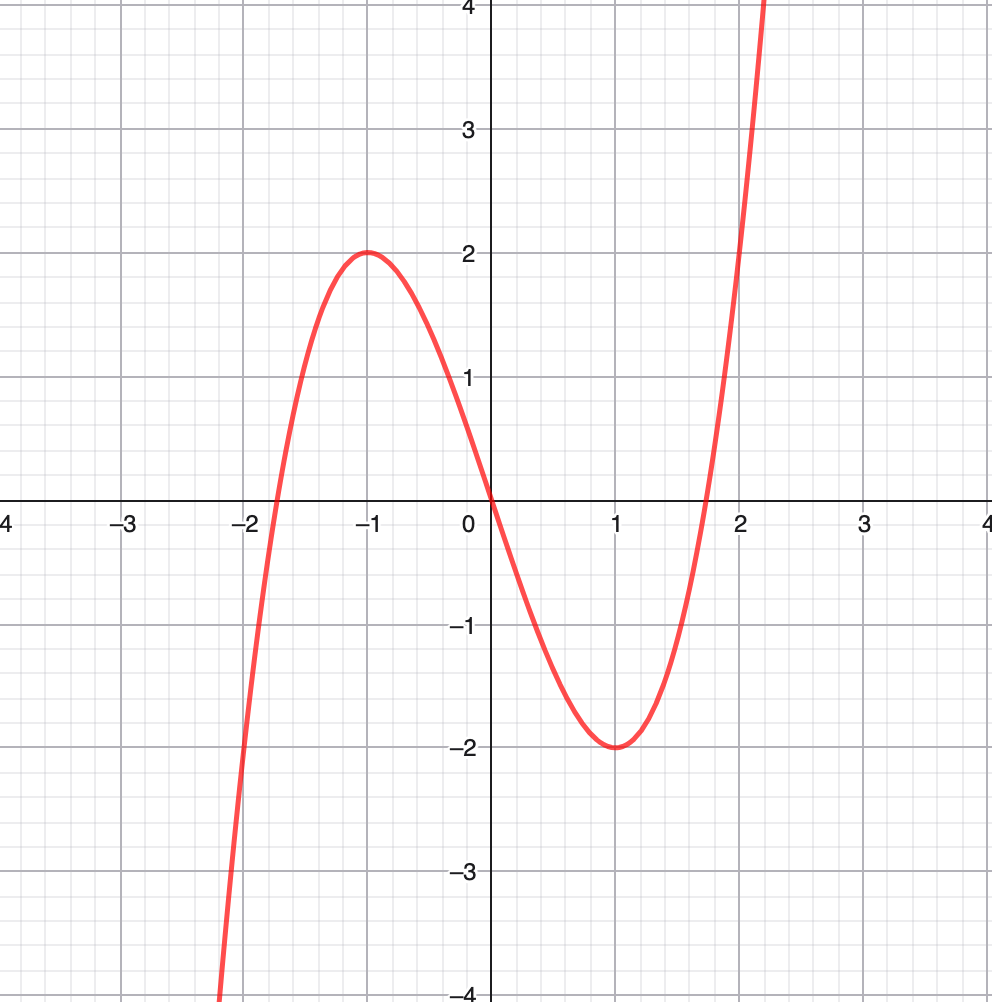
\includegraphics[scale=0.5,max width=\linewidth,max height=.72\textheight]{x^3-3x.png}
\end{center}
\end{example}
 $f'(x)$-ийн тэмдэгийг мэдснээр функцийн өсөлт–бууралтыг мэдэх төдийгүй улмаар локал болон глобал экстремумын байршлыг тодорхойлдог. 

 Фермагийн теорем экстремум байхгүй цэгүүдйиг зааж өгдөг теорем юм. Өөрөөр хэлбэл $f'(a)\neq 0$ бол $x=a$ цэг экстремум биш юм. Харин $f'(a)= 0$ эсвэл $f'(a)$ оршин байхгүй бол $x=a$ цэг экстремум байж магадгүй.
\end{frame}

\begin{frame}[allowframebreaks]{Өсөлт, бууралтын шинжилгээ}
 \begin{definition}
     Хэрэв $y=f(x)$ функцийн хувьд $f'(a)= 0$ эсвэл $f'(a)$ оршин байхгүй бол $x=a$ цэгийг $y=f(x)$ функцийн локал эксттермум байж магадгүй \textit{сэжигтэй цэг} гэнэ.
 \end{definition}
\end{frame}

\begin{frame}[allowframebreaks]{Өсөлт, бууралтын шинжилгээ}
\begin{example}
$f(x)=x e^{-x}$ бол
\[
f'(x)=e^{-x}(1-x) 
\] байна.
$e^{-x}>0$ тул $f'(x)$-ийн тэмдэгийг $1-x$ тодорхойлно:
\[
\begin{cases}
f'(x)>0, & x<1 \;\Rightarrow\; f \text{ өсөх},\\
f'(x)<0, & x>1 \;\Rightarrow\; f \text{ буурах}.
\end{cases}
\]
$f'(x)=e^{-x}(1-x)=0\Rightarrow x=1 $ тул сэжигтэй цэг нь $x=1$ болно. График харвал 
\begin{center}
    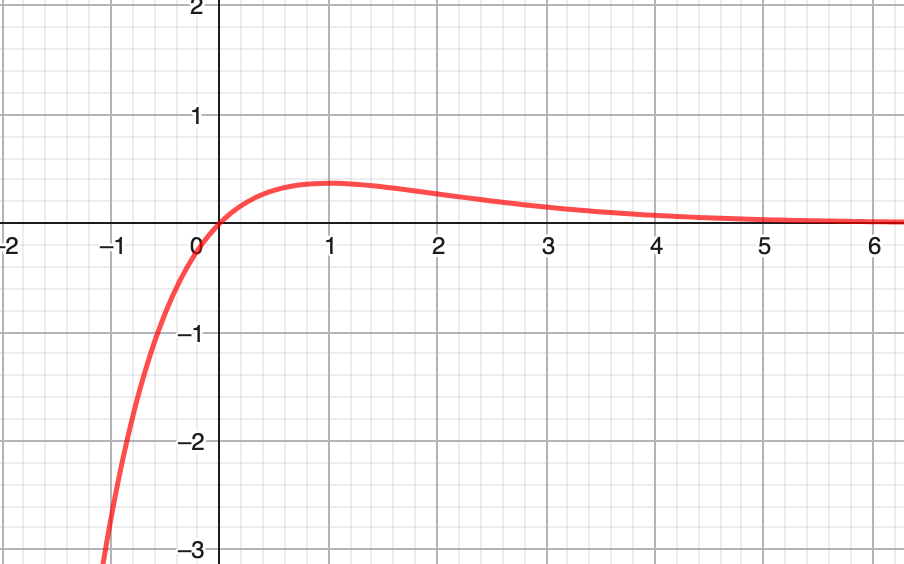
\includegraphics[scale=0.4,max width=\linewidth,max height=.72\textheight]{xe^-x.png}
\end{center} 
$x=1$ цэг нь локал максимум ба 
$f(1)=e^{-1}$ нь \textbf{локал максимум утга} байна.
\end{example}
Дээрх жишээнээс дараах дүгнэлт хийж болно. 
\end{frame}

\begin{frame}[allowframebreaks]{Өсөлт, бууралтын шинжилгээ}
\begin{theorem}
    $x=a$ цэг нь $y=f(x)$ функцийн сэжигтэй цэг байг. Хэрэв функц $(a-\delta;a)$ завсарт өсөөд (буураад), $(a;a+\delta)$ завсарт буурдаг (өсдөг) байх $\delta>0$ тоо олддог бол $x=a$ цэг $y=f(x)$ функцийн локал максимум (минимум)-н  цэг байна.
\end{theorem}
\end{frame}

\begin{frame}[allowframebreaks]{Өсөлт, бууралтын шинжилгээ}
\begin{example}
$f(x)=x^2 e^{-x}$.
\[
f'(x)=e^{-x}(2x-x^2)=e^{-x}x(2-x).
\]
$f'(x)$-ийн тэмдэг:
\begin{itemize}
  \item $x<0$: $f'(x)<0$ (буурах),
  \item $0<x<2$: $f'(x)>0$ (өсөх),
  \item $x>2$: $f'(x)<0$ (буурах).
\end{itemize}
Тиймээс $x=0$ дээр \textbf{локал минимум}, $x=2$ дээр \textbf{локал максимум}.
\[
f(0)=0,\qquad f(2)=4e^{-2}.
\]
\end{example}
\begin{center}
\begin{fitbox}\begin{tikzpicture}[scale=1.0]
\begin{axis}[
  width=12cm,height=7cm,
  axis lines=middle,
  xlabel={$x$},ylabel={$y$},
  xmin=-1.5,xmax=5,
  ymin=-0.5,ymax=1,
  samples=200,domain=-1.5:5,
  smooth,thick
]
\addplot[blue] {x^2*exp(-x)};
\addplot[dashed,gray] coordinates {(0,0) (0,0)};
\addplot[dashed,gray] coordinates {(2,0) (2,{4*exp(-2)})};
\node[above left] at (axis cs:0.8,0) {$x=0$ (min)};
\node[above] at (axis cs:2,{4*exp(-2)}) {$x=2$ (max)};
\end{axis}
\end{tikzpicture}\end{fitbox}
\end{center}
\end{frame}

\begin{frame}[allowframebreaks]{Өсөлт, бууралтын шинжилгээ}
\begin{example}
$f(x)=|x|$ функцийн график “V” хэлбэртэй байдаг. 

\[
f(x)=
\begin{cases}
 -x, & x<0,\\[3pt]
  x, & x\ge 0.
\end{cases}
\]
тул уламжлал нь
\[
f'(x)=
\begin{cases}
 -1, & x<0,\\[3pt]
 +1, & x>0.
\end{cases}
\]
$x=0$ дээр $f'(x)$ оршихгүй ($\lim_{x\to0^-}f'(x)=-1$, $\lim_{x\to0^+}f'(x)=1$), учир $x=0$ — сэжигтэй цэг болно.

\textbf{Өсөлт–бууралтын шинжилгээ:}
\begin{itemize}
  \item $x<0$ үед $f'(x)=-1<0$ → $f$ \textbf{буурах}.
  \item $x>0$ үед $f'(x)=+1>0$ → $f$ \textbf{өсөх}.
\end{itemize}

Тиймээс $f(x)$ нь $x=0$ цэгт буурахаас өсөхөд шилжиж байна.
Иймд $x=0$ нь \textbf{локал минимум} ба $f(0)=0$.
\begin{center}
\begin{fitbox}\begin{tikzpicture}[scale=1.1]

% --- координатын тэнхлэг ---
\draw[->, thick] (-3.2,0) -- (3.2,0) node[right] {$x$};
\draw[->, thick] (0,-0.5) -- (0,3.2) node[above] {$y$};

% --- |x| функцийн график ---
\draw[blue, very thick] (-3,3) -- (0,0) -- (3,3);

% цэгийн тэмдэглэгээ
\node[below left] at (0,0) {$O(0,0)$};
\node[above right] at (1.7,1.4) {$f(x)=|x|$};


\end{tikzpicture}\end{fitbox}
\end{center}
Графикаас $x=0$ — локал болон глобаль минимум байна.
\end{example}

Энэ аргаар функцийн өсөлт–бууралтын завсар, түүгээр дамжуулан локал экстремумыг тодорхойлох аргийг \emph{1-р уламжлалын тэмдэгийн тест} гэж нэрлэдэг.
\end{frame}

\subsection{Экстермум олох}
\begin{frame}[allowframebreaks]{Экстермум олох}
$y=f(x)$ функцийн $[a,b]$ завсар дээрх локал экстермум олохын тулд дараах алхамуудыг гүйцэтгэх шаардлагатай.
\begin{enumerate}
  \item $f'(x)$ уламжлалыг олж түүний уламжлал оршихгүй цэгүүд болон $f'(x)=0$ тэгшитгэл бодож сэжигтэй цэгүүдийг олно. 
  \item \textit{I уламжлалын тестээр (тэмдэгийн хүснэгт):} Сэжигтэй цэг $c$-г дайрч гарахдаа $f'$-ийн тэмдэг өөрчлөгдөх байдлыг шалган локал максимум, локал минимум эсвэл экстермум биш эсэхийг тодорхойлоно. Хэрэв  $f'$-ийн тэмдэг $+\to -$ бол максимум, $-\to +$ бол минимум, тэмдэг өөрчлөгдөхгүй бол экстремум биш байна.
\end{enumerate}  
\end{frame}

\begin{frame}[allowframebreaks]{Экстермум олох}
\begin{example}
$f(x)=\dfrac{x+1}{x^2+1}$ \quad (муж $x\in\mathbb{R}$).
\[
f'(x)=\frac{(1)(x^2+1)-(x+1)(2x)}{(x^2+1)^2}
=\frac{x^2+1-2x(x+1)}{(x^2+1)^2}
=\frac{-x^2-2x+1}{(x^2+1)^2}.
\]
Сэжигтэй цэгүүд: $-x^2-2x+1=0 \;\Rightarrow\; x=\frac{-2\pm\sqrt{4+4}}{2}=-1\pm\sqrt{2}$.
Иймд $x=-1-\sqrt2$-д $f'$ тэмдэг $+\to -$ (максимум), $x=-1+\sqrt2$-д $-\to +$ (минимум) болно.
\[
f(-1-\sqrt2)=\frac{-\sqrt2}{( (-1-\sqrt2)^2+1)} \quad\text{ба}\quad
f(-1+\sqrt2)=\frac{\sqrt2}{( (-1+\sqrt2)^2+1)}.
\]
Дүгнэлт: $x=-1-\sqrt2$ дээр локал максимум, $x=-1+\sqrt2$ дээр локал минимум.
\end{example}

$y=f(x)$ функцийн $[a,b]$ завсар дээрх глобал экстермум олохын тулд дараах алхамуудыг гүйцэтгэх шаардлагатай.
\begin{enumerate}
  \item Локал экстермумийн цэгүүдийг олж локал экстремумын цэгүүд дээрх функцийн утгууд $f(c)$-г бодно.
  \item Төгсгөлүүдийн цэгүүд дээрх утгууд $f(a), f(b)$-г бодож экстремумын цэгүүд дээрх функцийн утгуудтай харьцуулан эдгээрээс глобал экстермум утгаа тодорхойлно.
  \end{enumerate}  
\end{frame}

\begin{frame}[allowframebreaks]{Экстермум олох}
\begin{example}
$f(x)=x^3-3x$-ийн глобал экстремумыг $[-2,2]$ дээр ол.
\[
f'(x)=3x^2-3=3(x^2-1)=0 \;\Rightarrow\; x=\pm1.
\]
Төгсгөлийн цэгүүд: $x=-2,\,2$. Утгууд:
\[
f(-2)=-8+6=-2,\quad f(-1)=-1+3=2,\quad f(1)=1-3=-2,\quad f(2)=8-6=2.
\]\\
\textbf{Дүгнэлт:} Хамгийн их утга $2$ нь $x=-1$ ба $x=2$ дээр; хамгийн бага утга $-2$ нь $x=-2$ ба $x=1$ дээр.    
\end{example}
\end{frame}

\begin{frame}[allowframebreaks]{Экстермум олох}
\begin{example}
$f(x)=x\,e^{-x^2}$-ийн глобал экстремумыг $\mathbb{R}$ дээр ол.
\[
f'(x)=e^{-x^2}(1-2x^2)=0 \;\Rightarrow\; x=\pm \frac{1}{\sqrt2}.
\]
Утгууд:
\[
f\!\left(\tfrac{1}{\sqrt2}\right)=\frac{1}{\sqrt2}\,e^{-1/2}=\frac{1}{\sqrt{2e}},\qquad
f\!\left(-\tfrac{1}{\sqrt2}\right)=-\frac{1}{\sqrt{2e}}.
\]
Мөн $\lim_{x\to\pm\infty}f(x)=0$. \\
\textbf{Дүгнэлт:} Хамгийн их утга $f_{\max}=\dfrac{1}{\sqrt{2e}}$ нь $x=\dfrac{1}{\sqrt2}$ дээр;хамгийн бага утга $f_{\min}=-\dfrac{1}{\sqrt{2e}}$ нь $x=-\dfrac{1}{\sqrt2}$ дээр.
\end{example}
\end{frame}

\begin{frame}[allowframebreaks]{Экстермум олох}
\begin{example}
$f(x)=|x|+(x-1)^2$-ийн абсолют экстремумыг $\mathbb{R}$ дээр ол.

Модулийг задлахын тулд хоёр мужид хуваая. 
\[
\begin{cases}
x\ge 0:\; f(x)=x+(x-1)^2 = x^2+(-1)x+1, \quad f'(x)=2x-1,\\[2pt]
x<0:\; f(x)=-x+(x-1)^2 = x^2-3x+1, \quad f'(x)=2x-3.
\end{cases}
\]
Сэжигтэй цэгүүд:
\[
x> 0:\; 2x-1=0 \Rightarrow x=\tfrac12\ (\text{тэгээс их тул шийд болно}),\]
\[
x<0:\; 2x-3=0 \Rightarrow x=\tfrac32\ \text{(энэ нь тэгээс бага биш тул шийд биш)}.
\]
Мөн $x=0$ дээр $|x|$-ийн уламжлал тасардаг тул сэжигтэй цэг болох тул \emph{заавал} шалгана.
Утгууд:
\[
f\!\left(\tfrac12\right)=\tfrac12+\Big(\tfrac12-1\Big)^2=\tfrac12+\tfrac14=\tfrac34,\qquad
f(0)=0+1=1.
\]
$x\to\pm\infty$ үед $f(x)\sim x^2\to\infty$. \\
\textbf{Дүгнэлт:} Хамгийн бага утга $f_{\min}=\dfrac{3}{4}$ нь $x=\dfrac12$ дээр, хамгийн их утга байхгүй (∞ руу өснө)    
\end{example} 
\end{frame}

\subsection{Лопиталын дүрэм}
\begin{frame}[allowframebreaks]{Лопиталын дүрэм}
\begin{theorem}[Лопитал]
$f,g$ нь $a$ цэгийн орчинд дифференциалчлагддаг, $g'(x)\ne0$, мөн $x\to a$ үед $f$ ба $g$ нь $0$ (эсвэл $\pm\infty$) руу ойртдог байг. Хэрэв
\[
\lim_{x\to a}\frac{f'(x)}{g'(x)}=L \text{ оршвол}\quad 
\lim_{x\to a}\frac{f(x)}{g(x)}=L.
\]
\end{theorem}

\begin{prof}
Кошийн теоремыг $[x,a]$ дээр хэрэглэн $\dfrac{f'(c)}{g'(c)}=\dfrac{f(x)-f(a)}{g(x)-g(a)}$ ($f(a)=g(a)=0$) авна. $x\to a$ үед $c\to a$.
\end{prof}
\end{frame}

\begin{frame}[allowframebreaks]{Лопиталын дүрэм}
\begin{example}
\begin{multicols}{2}
\begin{enumerate}[itemsep=2pt]
\item $\displaystyle \lim_{x\to0}\frac{\sin x}{x}=\lim\frac{\cos x}{1}=1.$
\item $\displaystyle \lim_{x\to\infty}\frac{\ln x}{x}=\lim\frac{1/x}{1}=0.$
\item $\displaystyle \lim_{x\to0}\frac{e^x-1}{x}=\lim\frac{e^x}{1}=1.$
\item $\displaystyle \lim_{x\to0}\frac{1-\cos x}{x^2}=\lim\frac{\sin x}{2x}=\frac12.$
\end{enumerate}
\end{multicols}
    
\end{example}
\end{frame}

\section*{Семинар}
\begin{frame}[allowframebreaks]{Семинар}
\begin{enumerate}
  \item Дифференциал ашиглан ойролцоогоор бод
  \begin{enumerate}
  \item  \(\sin(0.12)\). (Радианаар авч үзнэ.)
  \item \((1.02)^5\)
\end{enumerate}
  \item Шүргэгч ба нормаль шулууны тэгшитгэлийг ол.    
  \begin{enumerate}
      \item \(y=\sin x+\cos x\)-ийн \(x=\tfrac{\pi}{3}\) цэг дээрх 
  \item \(y=x^2-3x+2\)-ийн \(x=1\) цэг дээрх 
  \item  \(x=\cos t,\; y=\sin t\) \(t=\tfrac{\pi}{4}\) дээрх
  \end{enumerate}
    \item $y=\sqrt{2x-x^2}$ функц $(0;1)$  дээр өсдөг, $(1;2)$ дээр буурдаг болохыг харуул.
    \item $y=x^3+x$ өсдөг болохыг батал.
    \item Өсөх, буурах завсарыг ол.
    \begin{enumerate}
        \item $y=(x-2)^5(2x+1)^4$
        \item $y=x-e^x$
        \item $y=\dfrac{1-x+x^2}{1+x+x^2}$
        \item $y=xe^{-x}$
        \item $y=\dfrac{1}{\ln x}$
        \item $y=x^2-\ln x$
        \item $y=x-\sin 2x,\quad (0<x<\pi)$
        \item $y=x+\cos x$
    \end{enumerate}
    \item Локал экстермум ол.
    \begin{enumerate}
        \item $y=2x^3-3x^2$
        \item $y=2x^3-6x^2+18x-1$
        \item $y=x^2\cdot \sqrt{x^2+2}$
        \item $y=x-\ln (x+1)$
        \item $y=\sin x$
        \item $y=x\sin x+\cos x-\dfrac{x^2}{4}, \quad -\dfrac{\pi}{2}\leq x\leq \dfrac{\pi}{2}$
        \item $y=\dfrac{1+3x}{\sqrt{4+5x^2}}$
        \item $y=x-\ln(1+x^2)$
        \item $y=\sqrt[3]{(x^2-4)^2}$
        \item $y=2e^{3x}+3e^{-3x}$
    \end{enumerate}
    \item Глобал экстермум ол.
    \begin{enumerate}
        \item $y=x^4-2x^2+5, \quad [-2;2]$
        \item $y=x+2\sqrt{x} \quad [0;4]$
        \item $y=x^5-5x^4+5x^3+2,\quad [-1;1]$
        \item $y=\sqrt{100-x^2}, \quad [-6;8]$
        \item $y=\dfrac{1-x+x^2}{1+x+x^2}, \quad [0;1]$
        \item $y=x\sin x+\cos x-\dfrac{x^2}{4}, \quad -\dfrac{\pi}{2}\leq x\leq \dfrac{\pi}{2}$
        \item $y=\dfrac{1+3x}{\sqrt{4+5x^2}}, \quad [0;1]$
        \item $y=x-\ln(1+x^2)$
        \item $y=\sqrt[3]{(x^2-4)^2}, \quad [0;3]$
        \item $y=2e^{3x}+3e^{-3x}$
    \end{enumerate}
\end{enumerate}
\end{frame}

\section*{Гэрийн даалгавар}
\begin{frame}[allowframebreaks]{Гэрийн даалгавар}
\begin{enumerate}
  \item Функцийн локал экстремумыг ол.
  \begin{enumerate}
  \item  $y = x^3 - 6x^2 + 9x - 4$ 
  \item $y = 2x^3 - x^4$ 
  \item $y = x(x-1)^3(x-2)^3$ 
  \item $y = x + \dfrac{1}{x}$ 
  \item $y = \dfrac{2x}{1+x^2}$ 
  \item $y = \dfrac{x^3 - 3x + 2}{x^3 + 2x + 1}$ 
  \item $y = \sqrt{2x - x^3}$ 
  \item $y = x^3\sqrt[3]{x - 1}$ 
  \item $y = x e^{-x}$
  \item $y = \sqrt{x}\,\ln x$ 
  \item $y = \dfrac{(\ln x)^2}{x}$
  \item $y = \cos x + \dfrac{1}{2}\cos 2x$ 
  \item $y = \dfrac{10}{1 + \sin^2 x}$ 
  \item $y = \arctan x - \dfrac{1}{2}\ln(1 + x^2)$ 
  \item $y = e^x \sin x$ 
  \item $y = |x|\, e^{-|x-1|}$
  \end{enumerate}
\item Өгөгдсөн завсар дээрх хамгийн их ба хамгийн бага утгыг ол.
  \begin{enumerate}
  \item  $f(x) = 2x$, $[-1; 5]$ 
  \item $f(x) = x^2 - 4x + 6$, $[-3; 10]$ 
  \item $f(x) = |x^2 - 3x + 2|$, $[-10; 10]$ 
  \item $f(x) = x + \dfrac{1}{x}$, $[0.01; 100]$ 
  \item $f(x) = \sqrt{5 - 4x}$, $[-1; 1]$ 
  \end{enumerate}
\item Дараах тэнцэтгэл бишүүдийг функцийн хамгийн их ба бага утга олох замаар батла.
   \begin{enumerate}
   \item $|3x - x^3| \le 2$, хэрэв $|x| \le 2$
   \item $\dfrac{1}{2^{p-1}} \le x^p + (1-x)^p \le 1$, хэрэв $0 \le x \le 1$ ба $p>1$.
  \item $x^m (a-x)^n \le 
    \dfrac{m^m n^n}{(m+n)^{m+n}}\, a^{m+n}$, хэрэв $m>0$, $n>0$, $0\le x\le a$.
  \item $\dfrac{x+a}{2^{(n-1)/n}} \le \sqrt[n]{x^n+a^n} \le x+a$, хэрэв $x>0,\, a>0,\, n>1$.
  \item $|a\sin x + b\cos x| \le \sqrt{a^2+b^2}$.
  \item $\dfrac{2}{3} \le \dfrac{x^2+1}{x^3+x+1} \le 2$, бүх $x \in \mathbb{R}$-д.
   \end{enumerate}
\item $y=ax^2+bx+c$ параболын $x=p, x=q$ цэгүүд дээрх шүргэгч шулуунууд $x=\dfrac{p+q}{2}$ цэг дээр огтолцохыг батал.
\item $y=x^2$ параболын $x=p, x=q$ цэгүүд дээрх шүргэгч шулуунууд перпиндикуляр бол огтолцолын цэг нь $y=-\dfrac{1}{4}$ шулуун дээр оршихыг батал.
\item $y=\dfrac{1}{x}$ функцийн $x=p ,\quad (p>0)$ цэг дээрх шүргэгч шулуун ба $ox$, $oy$ тэнхлэгүүдээр үүсэх гурвалжны талбай $p$-с хамаарахгүй тогтмол байхыг батал.
\end{enumerate}
\end{frame}
% Лекц 12. Хотгор, гүдгэр функц ба Тайлорын теорем
% Эх: latex/lectures/lec12-concavity-taylor.tex (scripts/latex_to_beamer.py-ээр хөрвүүлсэн)
% Frame бүр слайдад нэг (эсвэл allowframebreaks-аар хэд хэдэн) хуудас болно;
% хэвлэх хувилбарт frame-ийн хил харагдахгүй, текст үргэлжилсэн байна.

\MathLecture{12}{Хотгор, гүдгэр функц ба Тайлорын теорем}

\section{Хотгор ба гүдгэр функц}
\begin{frame}[allowframebreaks]{Хотгор ба гүдгэр функц}
\begin{definition}
Функц $y=f(x)$ нь $I=(a;b)$ завсар дээр 
$ \forall\,x_1,x_2\in I,\; \lambda\in[0,1]$ хувьд 
\[
  f(\lambda x_1 + (1-\lambda)x_2)
  \geq \lambda f(x_1) + (1-\lambda)f(x_2) \] тэнцэтгэл бишийг хангаж байвал $y=f(x)$ функцийг $I$ завсар дээр 
  \textbf{гүдгэр} (\emph{convex}) функц гэнэ. Хэрэв 
  \[
  f(\lambda x_1 + (1-\lambda)x_2)
  \leq \lambda f(x_1) + (1-\lambda)f(x_2), 
  \] тэнцэтгэл бишийг хангаж байвал $y=f(x)$ функцийг $I$ завсар дээр 
  \textbf{хотгор} (\emph{concave}) функц гэнэ.
\end{definition}
\end{frame}

\begin{frame}[allowframebreaks]{Хотгор ба гүдгэр функц}
\begin{example}
$f(x)=x^2$ функц дурын $I$ завсар дээр хотгор байхыг харуулая. Тодорхойлолтоор 
\[
f(\lambda x_1+(1-\lambda)x_2)
\leq
\lambda f(x_1)+(1-\lambda)f(x_2),
\qquad
x_1,x_2\in I,\ \lambda\in[0,1].
\]
байх ёстой.  $f(x)=x^2$ тул
\[
(\lambda x_1+(1-\lambda)x_2)^2
\le
\lambda x_1^2+(1-\lambda)x_2^2.
\]
Илэрхийлэлийг задлабал
\[
\lambda^2x_1^2+2\lambda(1-\lambda)x_1x_2+(1-\lambda)^2x_2^2
\le
\lambda x_1^2+(1-\lambda)x_2^2.
\]

Баруун талыг зүүн талаас хасвал:
\[
0
\le
\lambda(1-\lambda)(x_1-x_2)^2.
\]

Энэ нь бүх $x_1,x_2$ ба $\lambda\in[0,1]$ үед илт эерэг буюу $0$-оос их тэнцүү байна.  
Иймд тодорхойлолтоор
\[
\boxed{f(x)=x^2 \text{ нь бүх } \mathbb{R}\text{-д хотгор функц юм.}}
\]
\end{example}
\begin{center}
\begin{fitbox}\begin{tikzpicture}[scale=1.0]
  % Coordinate axes
  \draw[->] (-2.5,0) -- (2.5,0) node[right] {$x$};
  \draw[->] (0,-0.5) -- (0,3) node[above] {$y$};

  % Function y = x^2
  \draw[domain=-2:2.2, smooth, variable=\x, thick, blue]
    plot ({\x},{\x*\x}) node[right] {$y = x^2$};

  % Points x1 and x2
  \coordinate (A) at (-0.5,0.25);
  \coordinate (B) at (2,4);
  \fill (A) circle (1.5pt) node[left] {$A(x_1, f(x_1))$};
  \fill (B) circle (1.5pt) node[above right] {$B(x_2, f(x_2))$};

  % Chord between A and B
  \draw[very thick, red] (A) -- (B) node[midway, above, sloped] {хөвч};

  % Convex point
  \coordinate (C) at (1,1);
  \fill (C) circle (1.5pt) node[below right] {$C(\lambda x_1+(1-\lambda)x_2, f(\lambda x_1+(1-\lambda)x_2))$};
  \coordinate (D) at (1,2.5);
  % Dashed line showing function below chord
  \fill (D) circle (1.5pt) node[right] {$D(\lambda x_1+(1-\lambda)x_2,\lambda f(x_1)+(1-\lambda)f(x_2))$};
  \draw[dashed,red] (1,0) -- (D) node[midway, right] {};
\end{tikzpicture}\end{fitbox}
\end{center}
\end{frame}

\begin{frame}[allowframebreaks]{Хотгор ба гүдгэр функц}
\begin{theorem}[Хотгор, гүдгэр ба өсөлт бууралт]
    Хэрэв дифферинциалчлагдах $y=f(x)$ функц $(a;b)$  завсар дээр хотгор (гүдгэр ) бол түүний  уламжлал $(a;b)$ завсар дээр өснө (буурна).
\end{theorem}
\end{frame}

\begin{frame}[allowframebreaks]{Хотгор ба гүдгэр функц}
\begin{theorem}[Хотгор, гүдгэрийг тодорхойлоход уламжлал хэрэглэх]
Хэрэв $(a;b)$  завсар дээр $f''(x)$ хоёр дахь уламжлал оршин байдаг ба $\forall x\in (a;b)$ хувьд
\[
\begin{cases}
f''(x)>0 &\Rightarrow f \text{ хотгор},\\[4pt]
f''(x)<0 &\Rightarrow f \text{ гүдгэр}.
\end{cases}
\]
\end{theorem}

\begin{prof}
Лагранжийн дундаж утгын теорем ашиглая.
$x_1<x_2<x_3$ гурван цэг авбал,
\[
f'(x_2)-f'(x_1)=f''(c_1)(x_2-x_1),\qquad
f'(x_3)-f'(x_2)=f''(c_2)(x_3-x_2).
\]
Хэрэв $f''>0$ бол $f'$ өснө, иймээс графикийн шүргэгчүүдийн налалт өсдөг буюу график гүдгэр байна. $f''<0$ үед эсрэгээр.
\end{prof}
\end{frame}

\begin{frame}[allowframebreaks]{Хотгор ба гүдгэр функц}
\begin{definition}
    $y=f(x)$ функц $(a;c)$ завсар дээр хотгор (гүдгэр ) , $(c;b)$ завсар дээр  гүдгэр  (хотгор)  бол $x=c$ цэгийг түүний нугаралтын цэг гэнэ.
\end{definition}
\end{frame}

\begin{frame}[allowframebreaks]{Хотгор ба гүдгэр функц}
\begin{example}
$f(x)=x^3$ функцийн $f''(x)=6x$ тул $(-\infty,0)$ д гүдгэр, $(0,+\infty)$ д хотгор байна. Иймд $x=0$ нугаралтын цэг байна.
\end{example}

\begin{center}
\begin{fitbox}\begin{tikzpicture}[scale=0.9]
  \draw[->] (-2,0)--(2,0) node[right]{$x$};
  \draw[->] (0,-3)--(0,3) node[above]{$y$};
  \draw[domain=-1.3:1.3,smooth,variable=\x,blue,thick]
    plot({\x},{\x*\x*\x});
  \node at (1.1,1.2){хотгор};
  \node at (-1.1,-1.2){гүдгэр};
  \coordinate (C) at (0,0);
  \fill (C) circle (1.5pt) node[below right]{нугаралт};
\end{tikzpicture}\end{fitbox}
\end{center}
\end{frame}

\section{локал экстремум ба хотгор/гүдгэр}
\begin{frame}[allowframebreaks]{локал экстремум ба хотгор/гүдгэр}
Локал максимумын цэгийн орчимд функц гүдгэр байх нь илэрхий. Иймд сэжигтэй цэгийн орчимд гүдгэр хотгор байгаагаар нь түүний ямар төрлийн цэг болохыг тодорхойлож болно.  
$x_0$ цэг нь $y=f(x)$ функцийн сэжигтэй цэг байг:
\begin{itemize}
  \item Хэрэв $f''(x_0)>0$ бол $x_0$ — локал \textbf{минимум}.
  \item Хэрэв $f''(x_0)<0$ бол $x_0$ — локал \textbf{максимум}.
  \item Хэрэв $f''(x_0)=0$, $f'''(x_0)\ne0$ бол $x_0$ — \textbf{нугаралтын цэг}.
\end{itemize}
\end{frame}

\begin{frame}[allowframebreaks]{локал экстремум ба хотгор/гүдгэр}
\begin{example}
$f(x)=x^4-4x^2$.
\[
f'(x)=4x^3-8x,\qquad f''(x)=12x^2-8.
\]
$f'(x)=0\Rightarrow x=0,\pm\sqrt2$.  
$f''(0)=-8<0$ → максимум,  
$f''(\pm\sqrt2)=16>0$ → минимум.
\end{example}

\begin{center}
\begin{fitbox}\begin{tikzpicture}[scale=0.8]
  \draw[->] (-3,0)--(3,0) node[right]{$x$};
  \draw[->] (0,-5)--(0,5) node[above]{$y$};
  \draw[domain=-2.2:2.2,smooth,variable=\x,blue,thick]
    plot({\x},{\x*\x*\x*\x - 4*\x*\x});
  \node at (-2,-4.2){мин};
  \node at (0,0.5){макс};
  \node at (2,-4.2){мин};
\end{tikzpicture}\end{fitbox}
\end{center}
\end{frame}

\subsection*{3. Тэйлорын теорем}
\begin{frame}[allowframebreaks]{3. Тэйлорын теорем}
\begin{theorem}[Тэйлор]
Хэрэв $f(x)$ нь $a$ цэгийн орчинд $(n+1)$ удаа тасралтгүй уламжлалтай бол $a$ цэгийн орчний $x$ цэгийн хувьд
\begin{equation}\label{Taylor ex}
    f(x)=f(a)+f'(a)(x-a)+\frac{f''(a)}{2!}(x-a)^2+\cdots+\frac{f^{(n)}(a)}{n!}(x-a)^n+R_n(x),
\end{equation}
энд 
\[
R_n(x)=\frac{f^{(n+1)}(c)}{(n+1)!}(x-a)^{n+1},\quad c\in(a,x)
\] байна. 

Хэрэв $x-a=h$ гэж тэмдэглэвэл \[
f(a+h)=f(a)+f'(a)h+\frac{f''(a)}{2!}h^2+\cdots+\frac{f^{(n)}(a)}{n!}h^n+R_n(x),
\] болно. $R_n(x)$-г үлдэгдэл гишүүний Лагранжийн хэлбэр гэнэ.

Энэхүү \ref{Taylor ex} задаргааг $a$ төвтэй Тэйлорын задаргаа гэдэг. 
\end{theorem}

\begin{prof}
$f(x)-P_n(x)$ ба $(x-a)^{n+1}$ хоёр функц $x=a$ дээр 0 утгатай.  
Лагранжийн дундаж утгын теоремийг $(n+1)$ удаа хэрэглэснээр
$a<c<x$ тийм $c$ оршин:
\[
\frac{f(x)-P_n(x)}{(x-a)^{n+1}}=\frac{f^{(n+1)}(c)}{(n+1)!}.
\]
\end{prof}
\end{frame}

\begin{frame}[allowframebreaks]{3. Тэйлорын теорем}
\begin{example}
$f(x)=\sqrt{1+x}$, $a=0$ гэж авъя.  
$f'(x)=\dfrac1{2\sqrt{1+x}},\;
f''(x)=-\dfrac1{4(1+x)^{3/2}}.$  
Тэгвэл
\[
f(x)\approx1+\frac{x}{2}-\frac{x^2}{8}.
\]
$\sqrt{1.1}\approx1+\frac{0.1}{2}-\frac{0.01}{8}=1.04875.$  
Бодит утга $1.0488$ — сайн дөхөлт.
\end{example}
\end{frame}

\begin{frame}[allowframebreaks]{3. Тэйлорын теорем}
\begin{remark}[Маклорены задаргаа]
\ref{Taylor ex} томьёонд $a=0$ үед гарах задаргааг Маклорены задаргаа гэдэг. 
\[
f(x)=\sum_{k=0}^{n}\frac{f^{(k)}(0)}{k!}\,x^k+ \frac{f^{(n+1)}(c)}{(n+1)!}\,x^{n+1}.
\]
Хэрэв $n\to\infty$ үед үлдэгдэл $R_{n}(x)\to 0$ бол Маклорены \emph{цуваа} гэдэг.
\end{remark}
\end{frame}

\begin{frame}[allowframebreaks]{3. Тэйлорын теорем}
\begin{example}[Алдааны үнэлгээ (Лагранж үлдэгдэл)]
$f(x)=e^x$, $a=0$, $n=3$ гэж авъя. Тэгвэл
\[
e^x=1+x+\frac{x^2}{2!}+\frac{x^3}{3!}+\underbrace{\frac{e^c}{4!}x^4}_{R_4(x)},\qquad c\in(0,x).
\]
Жишээ нь $x=0.1$ үед $|R_4(0.1)|=\dfrac{e^{c}}{24}\,0.1^4\le \dfrac{e^{0.1}}{24}\,0.1^4<2.1\times 10^{-6}=0.0000021$.
\end{example}
\end{frame}

\section{Үндсэн функцүүдийн Маклорены задаргаа}
\begin{frame}[allowframebreaks]{Үндсэн функцүүдийн Маклорены задаргаа}
Дараах задаргааг \ref{Taylor ex} ашиглан хялбар шалгаж болно.
\[
e^x \;=\; 1 + x + \frac{x^2}{2!} + \cdots + \frac{x^n}{n!} \;+\; R_{n+1}(x), 
\qquad x\in\mathbb{R}\]
\[R_{n+1}(x)=\frac{e^{c}}{(n+1)!}\,x^{\,n+1},\ \ c\in(0,x).
\]
\[
\sin x \;=\; x - \frac{x^3}{3!} + \frac{x^5}{5!} - \cdots + 
(-1)^{m}\frac{x^{2m+1}}{(2m+1)!} \;+\; R_{2m+1}(x), \qquad x\in\mathbb{R}
\]
\[
R_{2m+1}(x)=\frac{\sin^{(2m+2)}(c)}{(2m+2)!}\,x^{\,2m+2},\ \ c\in(0,x).
\]
\[
\cos x \;=\; 1 - \frac{x^2}{2!} + \frac{x^4}{4!} - \cdots + 
(-1)^{m}\frac{x^{2m}}{(2m)!} \;+\; R_{2m}(x), \qquad x\in\mathbb{R}
\]
\[
R_{2m}(x)=\frac{\cos^{(2m+1)}(c)}{(2m+1)!}\,x^{\,2m+1},\ \ c\in(0,x).
\]
\[
\ln(1+x) \;=\; x - \frac{x^2}{2} + \frac{x^3}{3} - \cdots + 
(-1)^{n-1}\frac{x^{n}}{n} \;+\; R_{n}(x), \qquad x\in(-1;1)
\]
\[
R_{n+1}(x)=\frac{\ln^{(n+1)}(1+c)}{(n+1)!}\,x^{\,n+1}
=\frac{(-1)^{n}\,n!}{(n+1)!}\,\frac{x^{\,n+1}}{(1+c)^{n+1}}
= (-1)^{n}\,\frac{x^{\,n+1}}{(n+1)\,(1+c)^{n+1}},\ \ c\in(0,x).
\]
\[
\arctan x \;=\; x - \frac{x^3}{3} + \frac{x^5}{5} - \cdots + 
(-1)^{m}\frac{x^{2m+1}}{2m+1} \;+\; R_{2m+1}(x), \qquad x\in(-1;1)
\]
\[
R_{2m+1}(x)=\frac{(\arctan)^{(2m+2)}(c)}{(2m+1)!}\,x^{\,2m+1},\ \ c\in(0,x).
\]
\[
(1+x)^{\alpha} \;=\; 1 + \alpha x + \frac{\alpha(\alpha-1)}{2!}x^2 + \cdots +
\frac{\alpha(\alpha-1)\cdots(\alpha-n+1)}{n!}\,x^n \;+\; R_{n}(x), \qquad x\in(-1;1)
\]
\[
R_{n}(x)=\frac{(1+x)^{\alpha\,(n+1)}(c)}{(n+1)!}\,x^{\,n+1}
=\frac{\alpha(\alpha-1)\cdots(\alpha-n)}{(n+1)!}\,(1+c)^{\alpha-n-1}\,x^{\,n+1},\ \ c\in(0,x).
\]
Дээрх задаргаанд $\alpha=-1, x=-t, n=\infty$ гэвэл 
\[
\frac{1}{1-t} \;=\; 1 + t + t^2 + \cdots + t^n +\cdots 
\]
болж бидний мэдэх төгсгөлгүй буурах геометрийн прогрессийн нийлбэр гарна. Бусад задаргаанд ч мөн адил $n=\infty$ авч үзвэл цуваа үүснэ.
\end{frame}

\begin{frame}[allowframebreaks]{Үндсэн функцүүдийн Маклорены задаргаа}
\begin{example}[Тэйлор $a=\pi/4$ төвтэй]
$f(x)=\sin x$ функцийн $a=\pi/4$ төвтэй $n=2$ задаргааг бич.

$f(\tfrac{\pi}{4})=\tfrac{\sqrt2}{2}$,\ $f'(\tfrac{\pi}{4})=\tfrac{\sqrt2}{2}$,\ $f''(\tfrac{\pi}{4})=-\tfrac{\sqrt2}{2}$ тул
\[
\sin x=\frac{\sqrt2}{2}+\frac{\sqrt2}{2}(x-\tfrac{\pi}{4})-\frac{\sqrt2}{4}(x-\tfrac{\pi}{4})^2+\frac{-\sin(c)}{3!}(x-\tfrac{\pi}{4})^3.
\] Хэрэв энэ задаргааг ашиглах болбол ихэвчлэн үлдэгдэл гишүүнийг орхин ойролцоо тооцоолол хийдэг. Учир нь $c$ тоо олдох л болохоос хэрхэн олохыг мэдэхгүй.
\end{example}
\end{frame}

\begin{frame}[allowframebreaks]{Үндсэн функцүүдийн Маклорены задаргаа}
\begin{example}[Маклорен 3-р зэргийн ойролцоо] $y=\ln(1+x)$ функцийг 3 зэргийн олон гишүүнтээр ойролцоогоор соль.\\
$\ln(1+x)=x-\dfrac{x^2}{2}+\dfrac{x^3}{3}+R_4(x)$,\quad 
$|R_4(x)|=|- \dfrac{x^4}{4(1+c)^4}|\leq \dfrac{x^4}{4}$ тул  $|\ln(1+x) - (x-\tfrac{x^2}{2}+\tfrac{x^3}{3})|\lesssim \dfrac{|x|^4}{4}$.
\end{example}
\end{frame}

\begin{frame}[allowframebreaks]{Үндсэн функцүүдийн Маклорены задаргаа}
\begin{example}[Тэйлороор ойролцоо бодох]
$\sqrt{1+x}=(1+x)^{1/2}=1+\frac{x}{2}-\frac{x^2}{8}+\frac{x^3}{16}+\cdots$ ($|x|<1$). 
Жишээ нь $\sqrt{9.1}=\sqrt{9}\sqrt{1+0.1/9}\approx 3\!\left(1+\frac{0.1}{18}-\frac{(0.1)^2}{8\cdot 9^2}\right)$.
\end{example}
\end{frame}

\section{Функц шинжлэн график байгуулах 4 алхам}
\begin{frame}[allowframebreaks]{Функц шинжлэн график байгуулах 4 алхам}
Уламжлал ашиглан функцийн графикийг байгуулахад нийлээд нарийн зурах боломжтой. Дараах алхамуудын дагуу гарфик байгуулдаг.
\end{frame}

\subsection*{Алхам 1. $f(x)$-ийн ерөнхий шинжилгээ (графикийн үндсэн мэдээлэл)}
\begin{frame}[allowframebreaks]{Алхам 1. $f(x)$-ийн ерөнхий шинжилгээ (графикийн үндсэн мэдээлэл)}
\begin{itemize}
  \item \textbf{Тодорхойлогдох муж} $D_f$: томъёоны хязгаарлалт (хориглогдох тоон утга, тэнцэтгэл биш).
  \item \textbf{Тэгш/Сондгой \& Үе}: 
  \[
    f(-x)\stackrel{?}{=}f(x)\;\;(\text{тэгш}), \qquad
    f(-x)\stackrel{?}{=}-f(x)\;\;(\text{сондгой}), \qquad
    f(x+T)\stackrel{?}{=}f(x).
  \]
  \item \textbf{Тэнхлэгтэй огтлол \& тэмдэг}: $f(x)=0$ тэгүүд, $\;f(x)\gtrless 0$ тэмдэгийн муж (тэнхлэгийн дээгүүр/доогуур).
  \item \textbf{Хязгаарууд (шаардлагатай бол)}: $x\to a,\;\pm\infty$ үед $\lim f(x)$, хэвтээ/босоо/ ташуу асимптот боломж.
\end{itemize}
\end{frame}

\subsection*{Алхам 2. Нэгдүгээр уламжлал: өсөлт/бууралт, локал экстеомум}
\begin{frame}[allowframebreaks]{Алхам 2. Нэгдүгээр уламжлал: өсөлт/бууралт, локал экстеомум}
\begin{itemize}
  \item \textbf{Сэжигтэй цэгүүд}: $f'(x)=0$ болон $f'$ оршихгүй цэгүүд.
  \item \textbf{Өсөлт/Бууралт}: $f'(x)\geq 0$ тэмдэгийн хүснэгт байгуулж завсар бүрт монотон чанарыг тогтооно.
  \item \textbf{Локал экстремум}: $f'$-ийн тэмдэг солигдох байдлаар local \(\max/\min\) цэгүүдийг олно.
\end{itemize}
\end{frame}

\subsection*{Алхам 3. Хоёрдугаар уламжлал: хотгор/гүдгэр, нугаралтын цэг}
\begin{frame}[allowframebreaks]{Алхам 3. Хоёрдугаар уламжлал: хотгор/гүдгэр, нугаралтын цэг}
\begin{itemize}
  \item \textbf{Хотгор/Гүдгэр}: $f''(x)\gtrless 0$ тэмдэгийн хүснэгт байгуулж завсар бүрийн хэлбэрийг тогтооно.
  \item \textbf{Нугаралтын цэг}: $f''(x)=0$ буюу $f''$ оршихгүй ба  хотгор гүдгэр солигдох цэгүүд.
\end{itemize}
\end{frame}

\subsection*{Алхам 4. Нэгтгэх хүснэгт \& График}
\begin{frame}[allowframebreaks]{Алхам 4. Нэгтгэх хүснэгт \& График}
\begin{itemize}
  \item Алхам 1–3 дахь бүх мэдээллээ нэг хүснэгтэд нэгтгээд,
  \item Тэгш/сондгой байдал, асимптот, $x$-тэнхлэгийг огтлох цэгүүд, өсөлт/бууралт, хотгор/гүдгэр,
        экстремум, нугаралтын цэгүүдийг тэмдэглэн \textbf{график} зурах.
\end{itemize}
\end{frame}

\subsection*{Нэгтгэх хүснэгтийн жишиг загвар}
\begin{frame}[allowframebreaks]{Нэгтгэх хүснэгтийн жишиг загвар}
\begin{center}
\renewcommand{\arraystretch}{1.2}
\begin{fitbox}\begin{tabular}{|c|c|c|c|c|c|}
\hline
Завсар & $f(x)$-ийн тэмдэг & $f'(x)$ тэмдэг & Монотон & $f''(x)$ тэмдэг & Хотгор/Гүдгэр \\
\hline
$(\;\;,\;\;)$ & $+$/$-$ & $+$/$-$ & Өснө/Буурна & $+$/$-$ & Гүдгэр/Хотгор \\
\hline
$\cdots$ & $\cdots$ & $\cdots$ & $\cdots$ & $\cdots$ & $\cdots$ \\
\hline
\end{tabular}\end{fitbox}
\end{center}
\end{frame}

\subsection*{Алхам 1. Ерөнхий шинжилгээ}
\begin{frame}[allowframebreaks]{Алхам 1. Ерөнхий шинжилгээ}
\begin{itemize}
  \item \textbf{Тодорхойлогдох муж:} $D_f=\mathbb{R}$.
  \item \textbf{Тэнхлэгтэй огтлол:} $f(0)=(0+1)e^0=1$ → $y$-тэнхлэгийг $(0,1)$ цэгт огтлоно.
  \item $f(x)=0 \ \Rightarrow\ (x+1)e^x=0 \ \Rightarrow\ x=-1$ → $x=-1$ дээр $x$-тэнхлэгийг огтлоно.
  \item \textbf{Тэмдэг:} $f(x)<0$ ⇔ $x<-1$, $f(x)>0$ ⇔ $x>-1$.
  \item \textbf{Хязгаарууд:} 
  \[
  \lim_{x\to -\infty} (x+1)e^x = 0^{-}, \qquad 
  \lim_{x\to +\infty} (x+1)e^x = +\infty.
  \]
\end{itemize}
\end{frame}

\subsection*{Алхам 2. Нэгдүгээр уламжлал (өсөлт, бууралт, экстремум)}
\begin{frame}[allowframebreaks]{Алхам 2. Нэгдүгээр уламжлал (өсөлт, бууралт, экстремум)}
\[
f'(x) = (x+1)'e^x + (x+1)(e^x)' = e^x + (x+1)e^x = e^x(x+2).
\]
\begin{itemize}
  \item $f'(x)=0$ ⇔ $x=-2$.
  \item $e^x>0$ бүх $x$-д, тэгэхээр $f'(x)$-ийн тэмдэг нь $(x+2)$-оор тодорхойлогдоно.
  \[
  f'(x)<0 \text{  үед } x<-2, \qquad f'(x)>0 \text{  үед } x>-2.
  \]
  \item $\Rightarrow$ $x=-2$ нь \textbf{local минимум}.
  \item $f(-2)=(-1)e^{-2}=-\dfrac{1}{e^2}\approx -0.135$.
\end{itemize}
\end{frame}

\subsection*{Алхам 3. Хоёрдугаар уламжлал (хотгор, гүдгэр, нугаралт)}
\begin{frame}[allowframebreaks]{Алхам 3. Хоёрдугаар уламжлал (хотгор, гүдгэр, нугаралт)}
\[
f''(x) = \frac{d}{dx}[e^x(x+2)] = e^x(x+2)+e^x=e^x(x+3).
\]
\begin{itemize}
  \item $f''(x)=0$ ⇔ $x=-3$ → нугаралтын цэг.
  \item $f''(x)<0$ ($x<-3$) → хотгор, $f''(x)>0$ ($x>-3$) → гүдгэр.
  \item $\Rightarrow$ $x=-3$ нь нугаралтын цэг.
\end{itemize}
\end{frame}

\subsection*{Алхам 4. Мэдээллийг нэгтгэн хүснэгтэд оруулж график байгуулах}
\begin{frame}[allowframebreaks]{Алхам 4. Мэдээллийг нэгтгэн хүснэгтэд оруулж график байгуулах}
\begin{center}
\renewcommand{\arraystretch}{1.3}
\begin{fitbox}\begin{tabular}{|c|c|c|c|c|c|}
\hline
Завсар & $f(x)$ тэмдэг & $f'(x)$ тэмдэг & Өсөлт/Бууралт & $f''(x)$ тэмдэг & Хотгор/Гүдгэр \\
\hline
$(-\infty,-3)$ & $-$ & $-$ & Буурна & $-$ & Хотгор \\
\hline
$(-3,-2)$ & $-$ & $-$ & Буурна & $+$ & Гүдгэр \\
\hline
$(-2,\infty)$ & $+$ & $+$ & Өснө & $+$ & Гүдгэр \\
\hline
\end{tabular}\end{fitbox}
\end{center}
\end{frame}

\subsection*{График}
\begin{frame}[allowframebreaks]{График}
\begin{center}
\begin{fitbox}\begin{tikzpicture}[scale=1.0]
  % Тэнхлэгүүд
  \draw[->] (-5,0)--(3,0) node[below right] {$x$};
  \draw[->] (0,-2)--(0,5) node[above left] {$y$};

  % Функцийн муруй
  \draw[smooth,domain=-5:1,samples=200,thick,blue] plot(\x,{(\x+1)*exp(\x)});

  % Тэмдэглэсэн цэгүүд
  \fill (-2,{-1/exp(2)}) circle (2pt) node[below left] {$(-2,-\frac{1}{e^2})$};
  \fill (0,1) circle (2pt) node[above right] {$(0,1)$};
  \fill (-1,0) circle (2pt) node[below left] {$( -1,0)$};
  \draw[dashed] (-2,0)--(-2,{-1/exp(2)})--(0,{-1/exp(2)});

  % Тайлбарууд
  \node at (-4,3.5) {\small $f(x)=(x+1)e^x$};
  \node[blue] at (-2.5,-1.4) {\small Мин цэг};
  \node[blue] at (-3.2,0.8) {\small Хотгор};
  \node[blue] at (-1,3) {\small Гүдгэр};
\end{tikzpicture}\end{fitbox}
\end{center}
\end{frame}

% Семинар ба гэрийн даалгавар (Берманы бодлогын хураамжаас)
% Лекц 12: семинар ба гэрийн даалгавар. Бодлогууд: Г.Н. Берман, "Сборник задач по курсу
% математического анализа" (22-р хэвлэл). [Б.N] нь номын бодлогын дугаар.
% Тэмдэглэл: Берманы "вогнутый" = манай "гүдгэр" ($f''>0$), "выпуклый" = "хотгор" ($f''<0$).

\ProblemSet{Семинар 12}
\begin{frame}[allowframebreaks]{Семинар 12}
\pgroup{Хоёрдугаар эрэмбийн уламжлал ашиглан экстремумыг ол.}
\begin{plist}
\prob{1267}{$y=x^3-2ax^2+a^2x$ \ ($a>0$)}
\prob{1273}{$y=x^2e^{-x}$}
\end{plist}
\pgroup{Гүдгэр, хотгор завсар ба нугаралтын цэг.}
\begin{plist}
\prob{1281}{$4y=x\arctg x$ функцийн график хаа сайгүй гүдгэр болохыг харуул.}
\prob{1282}{$y=\ln(x^2-1)$ функцийн график хаа сайгүй хотгор болохыг харуул.}
\prob{1287}{$y=x^3-5x^2+3x-5$}
\prob{1289}{$y=x^4-12x^3+48x^2-50$}
\prob{1296}{$y=\ln(1+x^2)$}
\prob{1299}{$y=e^{\arctg x}$}
\prob{1305}{$a$ ба $b$ ямар утгатай үед $(1,3)$ цэг $y=ax^3+bx^2$ муруйн нугаралтын цэг болох вэ?}
\end{plist}
\pgroup{Асимптотыг ол.}
\begin{plist}
\prob{1377}{$y=\frac{1}{x^2-4x+5}$}
\prob{1379}{$2y(x+1)^2=x^3$}
\prob{1387}{$y=xe^x$}
\end{plist}
\pgroup{Функцийг бүрэн судалж графикийг байгуул.}
\begin{plist}
\prob{1398}{$y=\frac{x}{1+x^2}$}
\prob{1400}{$y=\frac{x}{x^2-1}$}
\prob{1408}{$y=\frac{x^3}{3-x^2}$}
\prob{1419}{$y=x-\ln(x+1)$}
\end{plist}
\pgroup{Тейлорын томьёо.}
\begin{plist}
\prob{1498}{$x^4-5x^3+x^2-3x+4$ олон гишүүнтийг $x-4$-ийн зэргээр задал.}
\prob{1504}{$y=xe^x$ функцийн $x_0=0$ цэг дээрх $n$-р эрэмбийн Тейлорын (Маклорены) томьёог бич.}
\prob{1505}{$y=\sqrt x$ функцийн $x_0=4$ цэг дээрх $n$-р эрэмбийн Тейлорын томьёог бич.}
\prob{1510}{$y=\tg x$ функцийн $x_0=0$ цэг дээрх 2-р эрэмбийн Тейлорын томьёог бич.}
\end{plist}
\end{frame}

\ProblemSet{Гэрийн даалгавар 12}
\begin{frame}[allowframebreaks]{Гэрийн даалгавар 12}
\pgroup{Хоёрдугаар эрэмбийн уламжлал ашиглан экстремумыг ол.}
\begin{plist}
\prob{1268}{$y=x^2(a-x)^2$}
\prob{1270}{$y=x+\sqrt{1-x}$}
\prob{1271}{$y=x\sqrt{2-x^2}$}
\prob{1276}{$a$-ийн ямар утгад $f(x)=a\sin x+\frac13\sin3x$ функц $x=\frac{\pi}{3}$ цэг дээр экстремумтай вэ? Энэ нь максимум уу, минимум уу?}
\prob{1277}{$y=a\ln x+bx^2+x$ функц $x_1=1$, $x_2=2$ цэгүүдэд экстремумтай байх $a,b$-г ол. Энэ үед $x_1$ дээр минимум, $x_2$ дээр максимум болохыг харуул.}
\end{plist}
\pgroup{Нугаралтын цэг, гүдгэр ба хотгор завсрыг ол.}
\begin{plist}
\prob{1288}{$y=(x+1)^4+e^x$}
\prob{1290}{$y=x+36x^2-2x^3-x^4$}
\prob{1292}{$y=(x+2)^6+2x+2$}
\prob{1293}{$y=\frac{x^3}{x^2+3a^2}$ \ ($a>0$)}
\prob{1294}{$y=a-\sqrt[3]{x-b}$}
\prob{1300}{$y=x^4(12\ln x-7)$}
\prob{1301}{$y=\frac{x+1}{x^2+1}$ муруй нэг шулуун дээр орших гурван нугаралтын цэгтэйг харуул.}
\prob{1307}{$a$-ийн ямар утгад $y=e^x+ax^3$ функцийн график нугаралтын цэгтэй вэ?}
\end{plist}
\pgroup{Асимптотыг ол.}
\begin{plist}
\prob{1378}{$y=c+\frac{a^3}{(x-b)^2}$}
\prob{1386}{$y=x\ln\bigl(e+\frac1x\bigr)$}
\prob{1388}{$y=xe^{2/x}+1$}
\prob{1390}{$y=2x+\arctg\frac{x}{2}$}
\end{plist}
\pgroup{Функцийг бүрэн судалж графикийг байгуул.}
\begin{plist}
\prob{1399}{$y=\frac{1}{1-x^2}$}
\prob{1402}{$y=\frac{x^2}{x^2-1}$}
\prob{1405}{$y=\frac1x+4x^2$}
\prob{1409}{$y=\frac{x^3}{2(x+1)^2}$}
\prob{1416}{$y=\frac{x}{e^x}$}
\prob{1420}{$y=\ln(x^2+1)$}
\prob{1423}{$y=xe^{-x^2/2}$}
\prob{1427}{$y=x+\sin x$}
\end{plist}
\pgroup{Тейлорын томьёо.}
\begin{plist}
\prob{1499}{$x^3+3x^2-2x+4$ олон гишүүнтийг $x+1$-ийн зэргээр задал.}
\prob{1503}{$y=\frac1x$ функцийн $x_0=-1$ цэг дээрх $n$-р эрэмбийн Тейлорын томьёог бич.}
\prob{1508}{$y=\sin^2x$ функцийн $x_0=0$ цэг дээрх $2n$-р эрэмбийн Тейлорын томьёог бич.}
\prob{1514}{$y=2x^6-x^3+3$ функцийн $x=0$ цэгийн орчим дахь төлөвийг Тейлорын томьёогоор тогтоо.}
\prob{1528}{$\ln(1+x)\approx x-\frac{x^2}{2}+\frac{x^3}{3}-\frac{x^4}{4}$ томьёогоор $\ln1{,}5$-г олж, алдааг үнэл.}
\end{plist}
\end{frame}


  % Лекц 13. Тодорхойгүй интеграл ба эх функц
% Эх: latex/lectures/lec13-antiderivative.tex (scripts/latex_to_beamer.py-ээр хөрвүүлсэн)
% Frame бүр слайдад нэг (эсвэл allowframebreaks-аар хэд хэдэн) хуудас болно;
% хэвлэх хувилбарт frame-ийн хил харагдахгүй, текст үргэлжилсэн байна.

\MathLecture{13}{Тодорхойгүй интеграл ба эх функц}

\section{Уламжлалын урвуу үйлдэл. Эх функц}
\begin{frame}[allowframebreaks]{Уламжлалын урвуу үйлдэл. Эх функц}
\begin{definition}
 $f(x)$ функц өгөгдсөн байг. Хэрэв $\Phi'(x)=f(x)$ бол $\Phi(x)$-ийг $f(x)$ функцийн
\emph{эх функц} гэнэ.   
\end{definition}
\end{frame}

\begin{frame}[allowframebreaks]{Уламжлалын урвуу үйлдэл. Эх функц}
\begin{example}
    $(x^2+x-1)'=2x+1$ тул $x^2+x-1$ нь $2x+1$ функцийн эх функц юм.
\end{example}
\end{frame}

\begin{frame}[allowframebreaks]{Уламжлалын урвуу үйлдэл. Эх функц}
\begin{theorem}\label{togtmol}
   Хэрэв $\forall x\in I$ дээр $f'(x)=g'(x)$ бол $\forall x\in I$ хувьд $f(x)-g(x)=C$ (тогтмол) байна.
 \end{theorem} 
\begin{prof} $h(x)=f(x)-g(x)$ гэе. 
$f'(x)=g'(x) \Rightarrow h'(x)=(f(x)-g(x))'=0$ болно. Лагранжийн теоремийн мөрдөлгөөгөөр   
 $$h'(x)=0 \Rightarrow h(x)=C.$$ Тэгэхээр
\[
f(x)=g(x)+C.
\]
\end{prof}
\end{frame}

\begin{frame}[allowframebreaks]{Уламжлалын урвуу үйлдэл. Эх функц}
\begin{definition}
 $f(x)$ функц өгөгдсөн байг. Түүний бүх эх функцүүдийн олонлогийг  $f(x)$ функцийн тодорхой биш интеграл гээд 
 $\displaystyle\int f(x)\,dx$ гэж тэмдэглэнэ. Th \ref{togtmol}-с 
 $$\int f(x)\,dx=\Phi(x)+C$$ байна. Энд $\Phi(x)$  ямар нэг эх функц.
 \end{definition}
\end{frame}

\section{Тодорхойгүй интегралын үндсэн жагсаалт}
\begin{frame}[allowframebreaks]{Тодорхойгүй интегралын үндсэн жагсаалт}
\begin{multicols}{2}
\begin{enumerate}
\item $\displaystyle\int x^n\,dx = \frac{x^{n+1}}{n+1}+C,\quad (n\neq -1)$
\item $\displaystyle\int \frac{dx}{x}= \ln |x|+C$
\item $\displaystyle\int e^x dx = e^x +C $
\item $\displaystyle\int a^x dx = \frac{a^x}{\ln a}+C$
\item $\displaystyle\int \sin x dx = -\cos x + C $
\item $\displaystyle\int \cos x dx = \sin x + C$
\item $\displaystyle\int \sec^2 x\, dx = \tan x +C$ 
\item $\displaystyle\int \frac{dx}{1+x^2}= \arctan x + C$
\item $\displaystyle\int \frac{dx}{\sqrt{1-x^2}} = \arcsin x +C$
\end{enumerate}
\end{multicols}
\end{frame}

\begin{frame}[allowframebreaks]{Тодорхойгүй интегралын үндсэн жагсаалт}
\begin{theorem}[ Арифметик үйлдлүүд ба эх функц] $f, \, g$ нь эх функцтэй бол, $C$ тогтмол тоо бол
  \begin{enumerate}
  \item $\displaystyle \int Cf\,dx=C\displaystyle \int f\,dx$ 
\item $\displaystyle \int (f\pm g)\,dx = \int f\,dx \pm \int g\,dx$
\item $\displaystyle \int f'(x)g(x)\,dx = f(x)g(x) - \int f(x)g'(x)\,dx$ (Хэсэгчлэн интегралчлах)
\item $\displaystyle \int f(g(x))g'(x)\,dx = \int f(u)\,du$ Энд $u=g(x)$,\quad (Орлуулах)
  \end{enumerate}
\end{theorem}
\end{frame}

\begin{frame}[allowframebreaks]{Тодорхойгүй интегралын үндсэн жагсаалт}
\begin{example}
\begin{enumerate}
\item $\displaystyle \int 3x^2\,dx=3\displaystyle \int x^2\,dx=3\dfrac{x^{2+1}}{2+1}+c=x^3+c$
\item $\displaystyle \int (3x^2 - 5\sqrt{x^3} + \dfrac{2}{x})\,dx=\displaystyle \int 3x^2 \,dx-\displaystyle \int  5\sqrt{x^3}\,dx+\displaystyle \int\dfrac{2}{x}\,dx=x^3-2x^{2.5}+2\ln x+C$
\item $
\displaystyle\int \sin^2\!\left(\frac{x}{2}\right)\,dx
= \int \frac{1-\cos x}{2}\,dx
= \frac12\int (1-\cos x)\,dx
= \frac{x}{2} - \frac{\sin x}{2} + C.
$
\end{enumerate}  
\end{example}
\end{frame}

\section{Орлуулах арга}
\begin{frame}[allowframebreaks]{Орлуулах арга}
\begin{theorem}[Орлуулах арга]\label{orluulah}
$\displaystyle\int f(u)\,du=F(u)+C$ ба $u=\varphi(x)$ нь дифференциалчлагддаг функц бол
\[
\int f\bigl(\varphi(x)\bigr)\varphi'(x)\,dx=F\bigl(\varphi(x)\bigr)+C .
\]
\end{theorem}
\begin{prof}
Давхар функцийн уламжлалын дүрмээр
$\bigl(F(\varphi(x))\bigr)'=F'(\varphi(x))\,\varphi'(x)=f(\varphi(x))\,\varphi'(x)$.
Иймд $F(\varphi(x))$ нь $f(\varphi(x))\varphi'(x)$ функцийн эх функц болно.
\end{prof}
\end{frame}

\begin{frame}[allowframebreaks]{Орлуулах арга}
$\varphi'(x)\,dx=d\varphi(x)$ тул теоремыг
\[
\int f\bigl(\varphi(x)\bigr)\,d\varphi(x)=\int f(u)\,du\Big|_{u=\varphi(x)}
\]
гэж бичиж болно. Үүнийг \emph{дифференциалын доор оруулах} гэж нэрлэдэг.
Ихэвчлэн хэрэглэгддэг хувиргалтууд:
\[
\renewcommand{\arraystretch}{1.6}
\begin{array}{ll@{\qquad}ll}
dx=\dfrac1a\,d(ax+b)\ (a\ne0), & & \dfrac{dx}{x}=d(\ln|x|), \\
x\,dx=\dfrac12\,d(x^2), & & e^x\,dx=d(e^x), \\
\cos x\,dx=d(\sin x), & & \dfrac{dx}{\cos^2x}=d(\tg x), \\
\sin x\,dx=-d(\cos x), & & \dfrac{dx}{2\sqrt x}=d(\sqrt x).
\end{array}
\]
\end{frame}

\begin{frame}[allowframebreaks]{Орлуулах арга}
\begin{cor}
$\displaystyle\int f(x)\,dx=F(x)+C$ бол
\begin{enumerate}
\item $\displaystyle\int f(ax+b)\,dx=\frac1a\,F(ax+b)+C$, \quad $a\ne0$;
\item $\displaystyle\int\frac{\varphi'(x)}{\varphi(x)}\,dx=\ln|\varphi(x)|+C$.
\end{enumerate}
\end{cor}
\end{frame}

\begin{frame}[allowframebreaks]{Орлуулах арга}
\begin{example}
\begin{enumerate}
\item $\displaystyle\int(3x-1)^5\,dx=\frac13\int(3x-1)^5\,d(3x-1)=\frac{(3x-1)^6}{18}+C$.
\item $\displaystyle\int\cos(2x+1)\,dx=\frac12\sin(2x+1)+C$.
\item $\displaystyle\int\frac{dx}{a^2+x^2}=\frac1a\int\frac{d(x/a)}{1+(x/a)^2}=\frac1a\arctg\frac xa+C$, \ ($a>0$).
\item $\displaystyle\int\frac{dx}{\sqrt{a^2-x^2}}=\int\frac{d(x/a)}{\sqrt{1-(x/a)^2}}=\arcsin\frac xa+C$, \ ($a>0$).
\end{enumerate}
\end{example}
\end{frame}

\begin{frame}[allowframebreaks]{Орлуулах арга}
\begin{example}
\begin{enumerate}
\item $\displaystyle\int x\,e^{x^2}dx$. \ $u=x^2$, $du=2x\,dx$ гэвэл
$\displaystyle\int x\,e^{x^2}dx=\frac12\int e^u\,du=\frac12e^{x^2}+C$.
\item $\displaystyle\int\tg x\,dx=\int\frac{\sin x}{\cos x}\,dx=-\int\frac{d(\cos x)}{\cos x}=-\ln|\cos x|+C$.
\item $\displaystyle\int\sin^3x\cos x\,dx=\int\sin^3x\,d(\sin x)=\frac{\sin^4x}{4}+C$.
\item $\displaystyle\int\frac{\ln x}{x}\,dx=\int\ln x\,d(\ln x)=\frac{\ln^2x}{2}+C$.
\item $\displaystyle\int\frac{2x+3}{x^2+3x+5}\,dx=\int\frac{d(x^2+3x+5)}{x^2+3x+5}=\ln(x^2+3x+5)+C$.
\end{enumerate}
\end{example}
\end{frame}

\begin{frame}[allowframebreaks]{Орлуулах арга}
\begin{theorem}[Хувьсагч солих]\label{huvsagch}
$x=\psi(t)$ нь $T$ завсар дээр дифференциалчлагддаг, хатуу монотон функц бөгөөд $t=\psi^{-1}(x)$ урвуутай байг. Хэрэв
$\displaystyle\int f\bigl(\psi(t)\bigr)\psi'(t)\,dt=G(t)+C$ бол
\[
\int f(x)\,dx=G\bigl(\psi^{-1}(x)\bigr)+C .
\]
\end{theorem}
\begin{prof}
Урвуу функцийн уламжлалаар $\bigl(\psi^{-1}(x)\bigr)'=\dfrac1{\psi'(t)}$. Иймд
$\bigl(G(\psi^{-1}(x))\bigr)'=G'(t)\cdot\dfrac1{\psi'(t)}=f(\psi(t))=f(x)$.
\end{prof}
\begin{remark}
Энэ аргад шинэ хувьсагчийг $x=\psi(t)$ хэлбэрээр сонгоно. Интегралчилсны дараа $t=\psi^{-1}(x)$-ийг орлуулж, анхны хувьсагч руу буцна.
\end{remark}
\end{frame}

\begin{frame}[allowframebreaks]{Орлуулах арга}
\begin{example}
$\displaystyle\int x\sqrt{x-1}\,dx$. \ $t=\sqrt{x-1}$ гэвэл $x=t^2+1$, $dx=2t\,dt$. Иймд
\[
\int x\sqrt{x-1}\,dx=\int(t^2+1)\,t\cdot2t\,dt=\frac{2t^5}{5}+\frac{2t^3}{3}+C
=\frac25(x-1)^{5/2}+\frac23(x-1)^{3/2}+C .
\]
\end{example}
\begin{example}
$\displaystyle\int\frac{dx}{1+\sqrt x}$. \ $x=t^2$ ($t\ge0$), $dx=2t\,dt$ гэвэл
\[
\int\frac{2t\,dt}{1+t}=2\int\Bigl(1-\frac1{1+t}\Bigr)dt=2t-2\ln(1+t)+C=2\sqrt x-2\ln(1+\sqrt x)+C .
\]
\end{example}
\end{frame}

\begin{frame}[allowframebreaks]{Орлуулах арга}
\begin{example}
$\displaystyle\int\sqrt{1-x^2}\,dx$. \ $x=\sin t$, $t\in[-\frac\pi2,\frac\pi2]$ гэвэл $dx=\cos t\,dt$, $\sqrt{1-x^2}=\cos t$. Иймд
\[
\int\sqrt{1-x^2}\,dx=\int\cos^2t\,dt=\int\frac{1+\cos2t}{2}\,dt=\frac t2+\frac{\sin2t}{4}+C .
\]
$\sin2t=2\sin t\cos t=2x\sqrt{1-x^2}$ тул
\[
\int\sqrt{1-x^2}\,dx=\frac12\arcsin x+\frac x2\sqrt{1-x^2}+C .
\]
\end{example}
\begin{remark}
$\sqrt{a^2-x^2}$ агуулсан интегралд $x=a\sin t$, \ $\sqrt{a^2+x^2}$ агуулсан интегралд $x=a\tg t$,
\ $\sqrt[n]{ax+b}$ агуулсан интегралд $t=\sqrt[n]{ax+b}$ орлуулгыг ихэвчлэн хэрэглэнэ.
\end{remark}
\end{frame}

\section{Хэсэгчлэн интегралчлах арга}
\begin{frame}[allowframebreaks]{Хэсэгчлэн интегралчлах арга}
$\displaystyle \int g'(x)f(x)\,dx = f(x)g(x) - \int g(x)f'(x)\,dx$ томьёог
\[
\int fdg = fg - \int g\,df
\] гэж бичиж болно. 

\textbf{Жишээ:}
$\int x e^x dx $ интегралд $f(x)=x, g'(x)dx=dg(x)=e^xdx=de^x$ гэвэл
\[
\int x e^x dx = xe^x - \int e^x dx = e^x(x -1)+C
\] болно. Хэрэв энд $f(x)=e^x, g'(x)dx=dg(x)=xdx=d\frac{x^2}{2}$ гэвэл
\[
\int x e^x dx = \frac{x^2}{2}e^x - \int \frac{x^2}{2}e^x dx
\] болно. Энэ гарсан интеграл нь өмнөхөөс хүнд харагдаж байна. Иймд хэсэгчлэх арга хэрэглэхэд $f, g'$ хэрхэн сонгох нь чухал юм.

\textbf{$f(x)$ сонгох дараалал (LAPTE):} Хэсэгчлэх арга хэрэглэхэд ихэвчлэн $f(x)$ функцийг дараах дараалалаар сонгоно.
\[
\text{Log} \rightarrow \text{Arc} \rightarrow \text{Polynomm} \rightarrow \text{Trig} \rightarrow \text{Exponential}
\]
\end{frame}

\begin{frame}[allowframebreaks]{Хэсэгчлэн интегралчлах арга}
\begin{example}
    $\displaystyle\int x\ln x \,dx$ бодоход LAPTE сонголтоор $\ln x$ байгаа тул түүнийг $f(x)=\ln x, g'(x)=x$ гэж авна. Иймд $g(x)=\dfrac{x^2}{2}$ болно. Иймд 
    $$\int x\ln x \,dx=\dfrac{x^2}{2}\ln x-\int \dfrac{x^2}{2}(\ln x)'dx=\dfrac{x^2}{2}\ln x-\int \dfrac{x^2}{2}\dfrac{1}{x}dx=\dfrac{x^2}{2}\ln x-\dfrac{x^2}{4}+c$$ болно.
\end{example}
\end{frame}

\begin{frame}[allowframebreaks]{Хэсэгчлэн интегралчлах арга}
\begin{example} $\int x^{2}e^{x}\,dx$ бодоход LAPTE сонголтоор $f(x)=x^2, g'(x)=e^x$ гэж авна. Иймд $g(x)=e^x$ болно.
 \[
\int x^{2}e^{x}\,dx
= x^{2}e^{x}-\int 2xe^{x}\,dx.
\] болно.
Сүүлийн $\displaystyle\int 2xe^{x}\,dx$ интегралыг мөн хэсэгчлэн интегралчилбал 
$$\int 2xe^{x}\,dx= 2xe^{x}-\int 2e^{x}\,dx$$ болно. Иймд 
\[
\int x^{2}e^{x}\,dx= x^{2}e^{x}-2xe^{x}+2e^{x}+C
= e^{x}(x^{2}-2x+2)+C.
\]
болно.
\end{example} 
\end{frame}

\begin{frame}[allowframebreaks]{Хэсэгчлэн интегралчлах арга}
\begin{example} $\displaystyle\int e^{x}\sin x\,dx $ интегралын хувьд  $f(x)=\sin x, g'(x)=e^x$ гэж авбал
    \[
\int e^{x}\sin x\,dx =e^x\sin x-\int e^x (-\cos x) dx
\]
болно. $\int e^x (-\cos x) dx$ интегралын хувьд  $f(x)=-\cos x, g'(x)=e^x$ гэж авбал

$$\int e^x (-\cos x) dx=e^x (-\cos x)-\int e^x(-\sin x) dx$$ болно. Хэрэв $I=\displaystyle\int e^{x}\sin x\,dx$ гэвэл 
$I=e^x\sin x-e^x\cos x-I$ болох тул $I=\dfrac{e^{x}}{2}(\sin x - \cos x) + C.$
\end{example}
\end{frame}

% Семинар ба гэрийн даалгавар (Берманы бодлогын хураамжаас)
% Лекц 13: семинар ба гэрийн даалгавар. Бодлогууд: Г.Н. Берман, "Сборник задач по курсу
% математического анализа" (22-р хэвлэл). [Б.N] нь номын бодлогын дугаар.

\ProblemSet{Семинар 13}
\begin{frame}[allowframebreaks]{Семинар 13}
\pgroup{Үндсэн жагсаалт ба энгийн хувиргалтаар интегралыг ол.}
\begin{plist}
\prob{1676}{$\int\sqrt x\,dx$}
\prob{1678}{$\int\frac{dx}{x^2}$}
\prob{1679}{$\int10^x\,dx$}
\prob{1685}{$\int(\sqrt x+1)(x-\sqrt x+1)\,dx$}
\prob{1688}{$\int\bigl(\frac{1-z}{z}\bigr)^2dz$}
\prob{1694}{$\int\frac{1+\cos^2x}{1+\cos2x}\,dx$}
\prob{1696}{$\int\tg^2x\,dx$}
\end{plist}
\pgroup{Дифференциалын доор оруулах (хувьсагч солих) аргаар ол.}
\begin{plist}
\prob{1706}{$\int(x+1)^{15}dx$}
\prob{1710}{$\int\sqrt{8-2x}\,dx$}
\prob{1713}{$\int x\sqrt{1-x^2}\,dx$}
\prob{1719}{$\int\sin^3x\cos x\,dx$}
\prob{1744}{$\int\tg x\,dx$}
\prob{1749}{$\int\frac{dx}{x\ln x}$}
\prob{1760}{$\int\frac{dx}{1+9x^2}$}
\prob{1761}{$\int\frac{dx}{\sqrt{4-x^2}}$}
\end{plist}
\pgroup{Хэсэгчлэн интегралчил.}
\begin{plist}
\prob{1833}{$\int x\cos x\,dx$}
\prob{1834}{$\int xe^{-x}dx$}
\prob{1836}{$\int x^n\ln x\,dx$ \ ($n\ne-1$)}
\prob{1837}{$\int x\arctg x\,dx$}
\prob{1860}{$\int e^x\sin x\,dx$}
\end{plist}
\end{frame}

\ProblemSet{Гэрийн даалгавар 13}
\begin{frame}[allowframebreaks]{Гэрийн даалгавар 13}
\pgroup{Үндсэн жагсаалт ба энгийн хувиргалтаар интегралыг ол.}
\begin{plist}
\prob{1681}{$\int\frac{dx}{2\sqrt x}$}
\prob{1683}{$\int3{,}4\,x^{-0{,}17}dx$}
\prob{1689}{$\int\frac{(1-x)^2}{x\sqrt x}\,dx$}
\prob{1690}{$\int\frac{(1+\sqrt x)^3}{\sqrt[3]{x}}\,dx$}
\prob{1693}{$\int\frac{3\cdot2^x-2\cdot3^x}{2^x}\,dx$}
\prob{1695}{$\int\frac{\cos2x}{\cos^2x\sin^2x}\,dx$}
\prob{1697}{$\int\ctg^2x\,dx$}
\prob{1698}{$\int2\sin^2\frac{x}{2}\,dx$}
\prob{1699}{$\int\frac{(1+2x^2)\,dx}{x^2(1+x^2)}$}
\end{plist}
\pgroup{Дифференциалын доор оруулах (хувьсагч солих) аргаар ол.}
\begin{plist}
\prob{1707}{$\int\frac{dx}{(2x-3)^5}$}
\prob{1712}{$\int2x\sqrt{x^2+1}\,dx$}
\prob{1715}{$\int\frac{x\,dx}{\sqrt{x^2+1}}$}
\prob{1720}{$\int\frac{\sin x\,dx}{\cos^2x}$}
\prob{1723}{$\int\frac{\sqrt{\ln x}}{x}\,dx$}
\prob{1724}{$\int\frac{(\arctg x)^2dx}{1+x^2}$}
\prob{1731}{$\int\sin(2x-3)\,dx$}
\prob{1738}{$\int\frac{dx}{2x-1}$}
\prob{1742}{$\int\frac{e^x\,dx}{e^x+1}$}
\prob{1752}{$\int e^{\sin x}\cos x\,dx$}
\prob{1755}{$\int e^{-3x+1}dx$}
\prob{1763}{$\int\frac{dx}{\sqrt{4-9x^2}}$}
\prob{1774}{$\int\frac{3x-1}{x^2+9}\,dx$}
\end{plist}
\pgroup{Хэсэгчлэн интегралчил.}
\begin{plist}
\prob{1832}{$\int x\sin2x\,dx$}
\prob{1838}{$\int\arccos x\,dx$}
\prob{1842}{$\int x\cos^2x\,dx$}
\prob{1849}{$\int x^2\ln(1+x)\,dx$}
\prob{1850}{$\int x^2e^{-x}dx$}
\prob{1855}{$\int\ln^2x\,dx$}
\prob{1858}{$\int(\arcsin x)^2dx$}
\prob{1862}{$\int e^{ax}\cos nx\,dx$}
\end{plist}
\end{frame}

% Лекц 14. Тодорхойгүй интеграл бодох
% Эх: latex/lectures/lec14-integration-techniques.tex (scripts/latex_to_beamer.py-ээр хөрвүүлсэн)
% Frame бүр слайдад нэг (эсвэл allowframebreaks-аар хэд хэдэн) хуудас болно;
% хэвлэх хувилбарт frame-ийн хил харагдахгүй, текст үргэлжилсэн байна.

\MathLecture{14}{Тодорхойгүй интеграл бодох}

\section{Рационал бутархайн интеграл}
\begin{frame}[allowframebreaks]{Рационал бутархайн интеграл}
$\dfrac{P(x)}{Q(x)}$ хэлбэрийн функцийг рационал функц гэдэг. Энд $P(x)$, $Q(x)$ нь олон гишүүнт. Хэрэв  $\deg P<\deg Q$ бол зөв рационал бутархай бусад үед засагдах рационал бутархай гэдэг. Хэрэв $\dfrac{P(x)}{Q(x)}$ засагдах рационал бутархай бол түүнийг 
$$\dfrac{P(x)}{Q(x)}=M(x)+\dfrac{R(x)}{Q(x)}$$ хэлбэрт нэг утгатай тавьж болно. Энд $M(x),\, R(x)$  олон гишүүнтүүд ба $\deg R<\deg Q$. Тиймээс зөв бутархайн интегралыг бодчихвол ямар ч рационал бутархай функцийн интегралыг бодож болно. 
\end{frame}

\begin{frame}[allowframebreaks]{Рационал бутархайн интеграл}
\begin{theorem}[Хялбар бутархайд задлах]
$\dfrac{P(x)}{Q(x)}$ зөв рационал бутархай бол түүнийг дараах 4 хэлбэрийн бутархайнуудын нийлбэрт нэг утгатай задлаж болно. Үүнд $p^2-4q<0$ ба 
 \begin{eqnarray}
\dfrac{A}{(x-a)}&&\text{-1-р төрлийн хялбар бутархай}\nonumber\\
\dfrac{A}{(x-a)^k}&&\text{-2-р төрлийн хялбар бутархай}\nonumber\\
\dfrac{A}{(x^2+px+q)}&&\text{-3-р төрлийн хялбар бутархай}\nonumber\\
\dfrac{A}{(x^2+px+q)^k}&&\text{-4-р төрлийн хялбар бутархай}\nonumber
\end{eqnarray}
\end{theorem}
Дээрх теоремээс харахад 4 төрлийн хялбар бутархайн интегралыг бодчихвол ямар ч рационал бутархайн интеграл бодогдоно. Эхлээд эдгээр интегралуудыг хэрхэн бодох талаар үзье. 
Хялбар бутархайн интегралууд дараах байдалтай:

\[
\int \frac{dx}{x-a}=\ln|x-a|+C,
\]

\[
\int \frac{dx}{(x-a)^n}=\frac{-1}{(n-1)(x-a)^{\,n-1}}+C,
\qquad n\ge 2,
\]

\[
\int\frac{dx}{x^2+a^2}=\frac{1}{a}\arctan\frac{x}{a}+C,
\]

\[
\int\frac{dx}{(x^2+px+q)}=\frac{2}{\sqrt{4q-p^2}}
\arctan\frac{2x+p}{\sqrt{4q-p^2}}+C.
\]

Хэрэв $x^2+px+q$ квадрат нь бодит язгуургүй бол түүнийг
\[
x^2+px+q=(x+a)^2+b^2
\]
хэлбэрт оруулж арктангенс ашиглан бодно.  Иймд 4-р төрлийн хялбар бутархайн интегралийн хувьд түүнийг $t=\dfrac{2x+p}{\sqrt{4q-p^2}}$ орлуулгаар $\dfrac{A}{(t^2+1)^n}$ хэлбэрт хувиргаж болно. Иймд
$$\displaystyle I_n = \int \frac{dx}{(1+x^2)^n}$$ хэрхэн бодохыг тайлбарлая.\\

Эхлээд $n=1$ үед
\[
I_1 = \int \frac{dx}{1+x^2} = \arctan x+C
\]
байхыг харах амархан. 

Хэсэгчлэн интегралчлах замаар
\[
I_n = \frac{x}{2(n-1)(1+x^2)^{n-1}} + \frac{2n-3}{2(n-1)} I_{n-1}
\]
томьёог гаргаж болно. Иймд 4-р төрлийн бутархайн интеграл бодогдоно. Жишээ болгон эхний хэдэн интегралыг бичвэл:
\[
I_2=\frac{x}{2(1+x^2)}+\frac12 I_1
   =\frac{x}{2(1+x^2)}+\frac12\arctan x+C
\]
$I_3$–г олохын тулд рекурент томьёонд $n=3$ гэж орлуулбал
\[
I_3=\frac{x}{2(1+x^2)^2}+\frac34 I_2
\] болно.
$I_2$–ийн оронд өмнө олсоноо орлуулбал:
\[
I_3=\frac{x}{2(1+x^2)^2}
    +\frac{3}{4}\left(\frac{x}{2(1+x^2)}+\frac12\arctan x\right)+C
\]
буюу
\[
I_3=
\frac{x}{2(1+x^2)^2}
+\frac{3x}{8(1+x^2)}
+\frac{3}{8}\arctan x+C
\]
болно.
$I_4$–г ижлээр олбол
\[
I_4=
\frac{x}{2(1+x^2)^3}
+\frac{5x}{12(1+x^2)^2}
+\frac{15x}{48(1+x^2)}
+\frac{15}{48}\arctan x+C.
\]
Бүх үзсэн зүйлсээ нэгтгэн үзвэл рационал бутархайн интегралыг бодохдоо дараах алхамуудыг хийнэ. 
\begin{enumerate}
    \item Эхний алхам рационал бутархайг засаж зөв бутархай ба олон гишүүнтийн нийлбэр болгоно.
    \item Зөв бутархайг хялбар рационал бутархайнуудын нийлбэр байдлаар илэрхийлэн.
    \item Интегралаа бодно.
\end{enumerate}
$\dfrac{R(x)}{Q(X)}$ зөв бутархайн хувьд
\begin{eqnarray}
Q(x)&=&A(x-a_1)\ldots (x-a_m)(x-b_1)^{n_1}\ldots (x-b_k)^{n_k}\nonumber\\
   &=& (x^2+p_1x+q_1)\ldots (x^2+p_lx+q_l)(x^2+r_1x+s_1)^{g_1}\ldots (x^2+p_dx+q_d)^{g_d}\nonumber
\end{eqnarray} бол түүнийг хялбар бутархайд задлахад $Q(x)$ олон гишүүнтийн зэрэгтэй тэнцүү тооний үл мэдэгдэх бүхий шугман тэгшитгэлийн систем бодно.
\end{frame}

\begin{frame}[allowframebreaks]{Рационал бутархайн интеграл}
\begin{example}
$$
\int\frac{3x^3+2x^2+x-7}{x^2+1} dx$$ хувьд

 \[
\frac{3x^3+2x^2+x-7}{x^2+1}
=
3x+2+\frac{-2x-9}{x^2+1}.
\]
болно. 
Энэ үед интеграл нь:
\[
\int (3x+2)\,dx - \int\frac{2x}{x^2+1}dx - 9\int\frac{dx}{x^2+1}=\dfrac{3}{2}x^2+2x-\ln(x^2+1)-9\arctan x+c.
\]   
\end{example} 
\end{frame}

\begin{frame}[allowframebreaks]{Рационал бутархайн интеграл}
\begin{example}
\[
\int \frac{dx}{x^2-1}
\]
бодъёо. Зөв бутархай учир хуваарийг үржигдэхүүн болговол ${x^2-1}=(x-1)(x+1)$ тул
\[
\frac{1}{(x-1)(x+1)}=\frac{A}{x-1}+\frac{B}{x+1}
\]
 байхаар $A, B$ олдоно. Ижил хуваарь өгвөл 
 \[
\frac{A}{x-1}+\frac{B}{x+1}=\frac{A(x+1)+B(x-1)}{(x-1)(x+1)}=\frac{(A+B)x+(A-B)}{(x-1)(x+1)}=\frac{1}{(x-1)(x+1)}
\] болно. Иймд 
$$
\begin{cases}
    A+B&=0\\
    A-B&=1
\end{cases}$$ болно. Үүнийг бодвол $A=0.5, B=-0.5$ болно. 
Тэгвэл интеграл
\[
\int \frac{dx}{x^2-1}=\frac12\Bigl[\int \Bigl(\dfrac{1}{x+1}-\dfrac{1}{x-1}\Bigr)dx\Bigr]==\frac12\ln|x-1|-\frac12\ln|x+1|+C
=\frac12\ln\left|\frac{x-1}{x+1}\right|+C.
\]
 болно.
\end{example}
\end{frame}

\begin{frame}[allowframebreaks]{Рационал бутархайн интеграл}
\begin{example}
 \[
\int \frac{dx}{x^2+4x+5}
=
\int \frac{dx}{(x+2)^2+1}
=
\arctan(x+2)+C.
\]   
\end{example}
\end{frame}

\begin{frame}[allowframebreaks]{Рационал бутархайн интеграл}
\begin{example}
Дараах интегралыг бод.
\[
I=\int\dfrac{2x^4 - x^3 - x^2 - 4x - 2}{x^3-x^2-x+1}\, dx.
\]

\textbf{1. Зөв бутархай болгох.}

Эхлээд олон гишүүнтийг үлдэгдэлтэй  хувааж зөв бутархайд шилжүүлнэ:
\[
\frac{2x^4 - x^3 - x^2 - 4x - 2}{x^3 - x^2 - x + 1}
= 2x+1 + \frac{2x^2 - 5x - 3}{x^3 - x^2 - x + 1}.
\]

Хуваарийг үржигдэхүүн болговол
\[
x^3 - x^2 - x + 1 
= x^2(x-1) -1(x-1)
= (x^2-1)(x-1)
= (x-1)^2(x+1).
\]

Тиймээс
\[
\frac{2x^4 - x^3 - x^2 - 4x - 2}{x^3 - x^2 - x + 1}
= 2x+1 + \frac{2x^2 - 5x - 3}{(x-1)^2(x+1)}.
\]


\textbf{2. Зөв бутархайг хялбар бутархайд задлах.}

Бутархайг
\[
\frac{2x^2 - 5x - 3}{(x-1)^2(x+1)}
= \frac{A}{x-1} + \frac{B}{(x-1)^2} + \frac{C}{x+1}
\]
гэж задлана.

Ижил хуваарь оруулбал:
\[
2x^2 - 5x - 3 
= A(x-1)(x+1) + B(x+1) + C(x-1)^2
= (A+C)x^2 + (B-2C)x + (-A+B+C).
\]
болно.
Коэффициентүүдийг харьцуулбал:
\[
2x^2 - 5x - 3 = (A+C)x^2 + (B-2C)x + (-A+B+C),
\]
ингээд систем:
\[
\begin{cases}
A + C = 2,\\
B - 2C = -5,\\
-\,A + B + C = -3.
\end{cases}
\]

Энэ системээс:
\[
A = 1,\qquad B = -3,\qquad C = 1.
\]

Иймээс
\[
\frac{2x^2 - 5x - 3}{(x-1)^2(x+1)}
= \frac{1}{x-1} - \frac{3}{(x-1)^2} + \frac{1}{x+1}.
\]

Тэгвэл бүхэлд нь
\[
\dfrac{2x^4 - x^3 - x^2 - 4x - 2}{x^3 - x^2 - x + 1}
= 2x+1 + \frac{1}{x-1} - \frac{3}{(x-1)^2} + \frac{1}{x+1}.
\]

\textbf{3. Хялбар бутархай тус бүрээр интегралчлах.}

Одоо
\[
\begin{aligned}
I
&= \int (2x+1)\,dx 
+ \int \frac{1}{x-1}\,dx 
- \int \frac{3}{(x-1)^2}\,dx 
+ \int\frac{1}{x+1}\,dx.
\end{aligned}
\]

\[
\int (2x+1)\,dx = x^2 + x + C_1,
\]

\[
\int\frac{1}{x-1}\,dx = \ln|x-1| + C_2,
\]

\[
\int \frac{3}{(x-1)^2}\,dx 
= 3\int (x-1)^{-2}\,dx 
= 3\cdot\frac{(x-1)^{-1}}{-1} 
= -\frac{3}{x-1},
\]
тэгэхээр
\[
-\int \frac{3}{(x-1)^2}\,dx = +\frac{3}{x-1},
\]

\[
\int\frac{1}{x+1}\,dx = \ln|x+1| + C_3.
\]

Иймээс
\[
I
= x^2 + x + \ln|x-1| + \frac{3}{x-1} + \ln|x+1| + C.
\]

Логарифмуудыг нэгтгээд
\[
I
= x^2 + x + \frac{3}{x-1} + \ln|x^2-1| + C,
\]
учир нь $x^2-1=(x-1)(x+1)$.

\end{example}
\end{frame}

\section{Иррационал функцийн интеграл}
\begin{frame}[allowframebreaks]{Иррационал функцийн интеграл}
Иррационал интеграл гэдэг нь интегралын тэмдэгтийн дор квадрат язгуур, ерөнхийдөө $x$-ийн бутархай зэрэг (\,$\sqrt{\phantom{x}}$, $\sqrt[n]{\phantom{x}}$\,) орсон интегралуудыг хэлнэ. Жишээлбэл:
\[
\int \sqrt{x+1}\,dx,\qquad 
\int \frac{dx}{\sqrt{x^2+4}},\qquad
\int \frac{x\,dx}{\sqrt{1-x^2}},\ \text{г.м.}
\]

Ийм интегралуудыг бодоход орлуулах арга түгээмэл ашиглана.
\end{frame}

\subsubsection*{1. $\sqrt{ax+b}$ хэлбэрийн иррационал интеграл}
\begin{frame}[allowframebreaks]{1. $\sqrt{ax+b}$ хэлбэрийн иррационал интеграл}
Ихэвчлэн $x$–ийг язгууртай тэнцүүлэх буюу
\[
 ax+b=t^2
\]
гэсэн орлуулга хэрэглэнэ.
\end{frame}

\begin{frame}[allowframebreaks]{1. $\sqrt{ax+b}$ хэлбэрийн иррационал интеграл}
\begin{example}
\[
\int \sqrt{x+1}\,dx.
\]

Орлуулая:
\[
x+1 = t^2 \quad\Rightarrow\quad x = t^2-1,\quad dx = 2t\,dt.
\]
Тэгвэл
\[
\sqrt{x+1} = \sqrt{t^2} = t \quad (t>0\ \text{мужийг авч болно}).
\]

Интеграл:
\[
\int \sqrt{x+1}\,dx
= \int t \cdot 2t\,dt
= 2\int t^2\,dt
= 2\cdot \frac{t^3}{3} + C
= \frac{2}{3}t^3 + C.
\]

Энд $t^2 = x+1$ тул $t=\sqrt{x+1}$:
\[
\int \sqrt{x+1}\,dx 
= \frac{2}{3}(x+1)^{3/2} + C.
\]
\end{example}
\end{frame}

\subsubsection*{2. $\sqrt{x^2+a^2}$ ба $\sqrt{x^2-a^2}$: тригонометр орлуулга}
\begin{frame}[allowframebreaks]{2. $\sqrt{x^2+a^2}$ ба $\sqrt{x^2-a^2}$: тригонометр орлуулга}
Квадрат язгуур дотор тэгш өнцөгт гурвалжин үүсгэж болохоор хэлбэр байвал тригонометр орлуулга ашиглана.

\begin{itemize}
  \item $\sqrt{x^2+a^2}$ үед $x = a\tan t$ гэж орлуулна.
  \item $\sqrt{x^2-a^2}$ үед $x = a\sec t$ (эсвэл $x=a\cosh t$ гэх мэт) гэж орлуулна.
  \item $\sqrt{a^2-x^2}$ үед $x = a\sin t$ гэж орлуулна.
\end{itemize}
\end{frame}

\begin{frame}[allowframebreaks]{2. $\sqrt{x^2+a^2}$ ба $\sqrt{x^2-a^2}$: тригонометр орлуулга}
\begin{example}
\[
\int \frac{dx}{\sqrt{x^2+4}}.
\]

Энд $x^2+4 = x^2+2^2$ тул $x=2\tan t$ гэж орлуулвал:
\[
x = 2\tan t \quad\Rightarrow\quad dx = 2\sec^2 t\,dt.
\]
Мөн
\[
\sqrt{x^2+4}
= \sqrt{4\tan^2 t + 4}
= 2\sqrt{\tan^2 t+1}
= 2\sec t.
\]

Интеграл:
\[
\int \frac{dx}{\sqrt{x^2+4}}
= \int \frac{2\sec^2 t\,dt}{2\sec t}
= \int \sec t\,dt.
\]

$\displaystyle \int \sec t\,dt = \ln|\sec t + \tan t| + C$ тул:
\[
\int \frac{dx}{\sqrt{x^2+4}}
= \ln|\sec t + \tan t| + C.
\]

Одоо $x$-руу буцаая. $x=2\tan t \Rightarrow \tan t = \dfrac{x}{2}$. 
Тэгвэл
\[
\sec t = \sqrt{1+\tan^2 t}
= \sqrt{1+\frac{x^2}{4}}
= \frac{\sqrt{x^2+4}}{2}.
\]

Ингээд
\[
\sec t + \tan t = \frac{\sqrt{x^2+4}}{2} + \frac{x}{2}
= \frac{\sqrt{x^2+4}+x}{2}.
\]

Тогтмол $\ln 2$-г $C$-д шингээж болдог тул:
\[
\int \frac{dx}{\sqrt{x^2+4}}
= \ln\bigl|\sqrt{x^2+4}+x\bigr| + C.
\]
\end{example}
\end{frame}

\subsubsection*{3. Дифференциал биномын интеграл (Чебышёвын теорем)}
\begin{frame}[allowframebreaks]{3. Дифференциал биномын интеграл (Чебышёвын теорем)}
Рациналь $m,n,p$ тоонуудын хувьд дараах интеграл
\[
\int x^{m}(a+b x^{n})^{p}\,dx
\]
ерөнхий тохиолдолд энгийн функцээр илэрхийлэгдэхгүй. Гэхдээ зөвхөн дараах
\textbf{гурван тусгай нөхцөл} биелэх үед рациональ функцийн интегралд шилжүүлж болдог. Үүнийг Чебышёвын теорем гэнэ.
\end{frame}

\subsection*{Тохиолдол 1. $p$ — бүхэл тоо}
\begin{frame}[allowframebreaks]{Тохиолдол 1. $p$ — бүхэл тоо}
Хэрэв
\[
p\in \mathbb{Z},
\]
бол 
\[
x = z^{N},
\]
орлуулга хэрэглэнэ. Энд $N$ нь $m$ болон $n$–ийн  \emph{ерөнхий хуваарь}.
\end{frame}

\subsection*{Тохиолдол 2. $\dfrac{m+1}{n}$ — бүхэл тоо}
\begin{frame}[allowframebreaks]{Тохиолдол 2. $\dfrac{m+1}{n}$ — бүхэл тоо}
Хэрэв
\[
\frac{m+1}{n}\in\mathbb{Z},
\]
бол дараах орлуулгыг хэрэглэнэ:
\[
a + b x^{n} = z^{N},
\]
энд $N$ нь $p$ бутархайн \emph{хуваарь}.
\end{frame}

\subsection*{Тохиолдол 3. $\dfrac{m+1}{n}+p$ — бүхэл тоо}
\begin{frame}[allowframebreaks]{Тохиолдол 3. $\dfrac{m+1}{n}+p$ — бүхэл тоо}
Хэрэв
\[
\frac{m+1}{n} + p \in \mathbb{Z},
\]
бол дараах орлуулга хэрэглэнэ:
\[
a x^{-n} + b = z^{N},
\]
энд мөн $N$ нь $p$ бутархайн хуваарь.
\end{frame}

\subsection*{Тайлбар}
\begin{frame}[allowframebreaks]{Тайлбар}
Хэрэв $n=1$ бол дээрх гурван нөхцөл нь дараахтай тэнцэнэ:
\begin{enumerate}
\item $p$ — бүхэл;
\item $m$ — бүхэл;
\item $m+p$ — бүхэл.
\end{enumerate}
\end{frame}

\subsection*{Жишээ}
\begin{frame}[allowframebreaks]{Жишээ}
Дараах интегралыг бодъё:
\[
\int x^3(2+x^4)^{1/2}\,dx.
\]

Энд $m=3$, $n=4$, $p=\frac12$. Шалгах:
\[
\frac{m+1}{n} = \frac{4}{4} = 1 \in \mathbb{Z},
\]
тиймээс \emph{Тохиолдол 2} биелж байна.

Орлуулга хийвэл:
\[
2 + x^4 = t^2, \qquad t = \sqrt{2+x^4}.
\]
Мөн
\[
4x^3\,dx = 2t\,dt \quad\Rightarrow\quad x^3dx = \frac{t}{2}\,dt.
\]

Интегралыг орлуулж бодъё:
\[
\int x^3(2+x^4)^{1/2}\,dx
= \int \left( \frac{t}{2}\right)t\,dt
= \frac12\int t^2 \, dt
= \frac{t^3}{6} + C.
\]

Буцааж орлуулбал:
\[
\boxed{
\int x^3(2+x^4)^{1/2}\,dx
= \frac{(2+x^4)^{3/2}}{6} + C.
}
\]
\end{frame}

% Семинар ба гэрийн даалгавар (Берманы бодлогын хураамжаас)
% Лекц 14: семинар ба гэрийн даалгавар. Бодлогууд: Г.Н. Берман, "Сборник задач по курсу
% математического анализа" (22-р хэвлэл). [Б.N] нь номын бодлогын дугаар.

\ProblemSet{Семинар 14}
\begin{frame}[allowframebreaks]{Семинар 14}
\pgroup{Бүхэл хэсгийг ялгах, бүтэн квадрат ялгах замаар ол.}
\begin{plist}
\prob{1781}{$\int\frac{x}{x+4}\,dx$}
\prob{1791}{$\int\frac{dx}{x(x-1)}$}
\prob{1796}{$\int\frac{dx}{x^2-7x+10}$}
\prob{1801}{$\int\frac{dx}{x^2+2x+3}$}
\prob{1805}{$\int\frac{dx}{\sqrt{4x-3-x^2}}$}
\end{plist}
\pgroup{Рационал бутархайн интеграл.}
\begin{plist}
\prob{2012}{$\int\frac{x\,dx}{(x+1)(2x+1)}$}
\prob{2014}{$\int\frac{2x^2+41x-91}{(x-1)(x+3)(x-4)}\,dx$}
\prob{2023}{$\int\bigl(\frac{x+2}{x-1}\bigr)^2\frac{dx}{x}$}
\prob{2027}{$\int\frac{dx}{x^4-x^2}$}
\prob{2036}{$\int\frac{dx}{x(x^2+1)}$}
\prob{2038}{$\int\frac{x\,dx}{x^3-1}$}
\prob{2039}{$\int\frac{(2x^2-3x-3)\,dx}{(x-1)(x^2-2x+5)}$}
\end{plist}
\pgroup{Иррационал функцийн интеграл.}
\begin{plist}
\prob{1872}{$\int\frac{dx}{x\sqrt{x+1}}$}
\prob{1874}{$\int\frac{dx}{1+\sqrt x}$}
\prob{1876}{$\int\frac{\sqrt x}{x+1}\,dx$}
\prob{1881}{$\int\frac{dx}{\sqrt x+\sqrt[4]{x}}$}
\prob{1891}{$\int\frac{x^2\,dx}{\sqrt{a^2-x^2}}$ \ (орлуулга $x=a\sin z$)}
\prob{1894}{$\int\frac{\sqrt{1-x^2}}{x^2}\,dx$}
\prob{1940}{$\int\frac{dx}{\sqrt{5-2x+x^2}}$}
\prob{1944}{$\int\frac{(x+2)\,dx}{x^2+2x+2}$}
\end{plist}
\end{frame}

\ProblemSet{Гэрийн даалгавар 14}
\begin{frame}[allowframebreaks]{Гэрийн даалгавар 14}
\pgroup{Бүхэл хэсгийг ялгах, бүтэн квадрат ялгах замаар ол.}
\begin{plist}
\prob{1784}{$\int\frac{3+x}{3-x}\,dx$}
\prob{1787}{$\int\frac{(1+x)^2}{x^2+1}\,dx$}
\prob{1790}{$\int\frac{x^4\,dx}{x^2+1}$}
\prob{1792}{$\int\frac{dx}{x(x+1)}$}
\prob{1793}{$\int\frac{dx}{(x+1)(2x-3)}$}
\prob{1797}{$\int\frac{dx}{x^2+3x-10}$}
\prob{1798}{$\int\frac{dx}{4x^2-9}$}
\prob{1803}{$\int\frac{dx}{4x^2+4x+5}$}
\prob{1806}{$\int\frac{dx}{\sqrt{8+6x-9x^2}}$}
\end{plist}
\pgroup{Рационал бутархайн интеграл.}
\begin{plist}
\prob{2015}{$\int\frac{dx}{6x^3-7x^2-3x}$}
\prob{2016}{$\int\frac{x^5+x^4-8}{x^3-4x}\,dx$}
\prob{2017}{$\int\frac{x^3-1}{4x^3-x}\,dx$}
\prob{2020}{$\int\frac{(2x^2-5)\,dx}{x^4-5x^2+6}$}
\prob{2024}{$\int\frac{x^2\,dx}{x^3+5x^2+8x+4}$}
\prob{2026}{$\int\frac{x^3-6x^2+11x-5}{(x-2)^4}\,dx$}
\prob{2028}{$\int\frac{x^2\,dx}{(x+2)^2(x+4)^2}$}
\prob{2041}{$\int\frac{x^2\,dx}{1-x^4}$}
\prob{2042}{$\int\frac{dx}{(x^2+1)(x^2+x)}$}
\prob{2044}{$\int\frac{(3x^2+x+3)\,dx}{(x-1)^3(x^2+1)}$}
\prob{2053}{$\int\frac{2x\,dx}{(1+x)(1+x^2)^2}$}
\end{plist}
\pgroup{Иррационал функцийн интеграл.}
\begin{plist}
\prob{1870}{$\int\frac{x^3\,dx}{\sqrt{x-1}}$}
\prob{1873}{$\int\frac{x+1}{x\sqrt{x-2}}\,dx$}
\prob{1877}{$\int\frac{dx}{1+\sqrt[3]{x+1}}$}
\prob{1880}{$\int\frac{dx}{\sqrt[3]{x}\,(\sqrt[3]{x}-1)}$}
\prob{1893}{$\int\frac{\sqrt{1+x^2}}{x^4}\,dx$}
\prob{1897}{$\int\frac{dx}{x^2\sqrt{x^2-9}}$}
\prob{1945}{$\int\frac{(x-3)\,dx}{\sqrt{3-2x-x^2}}$}
\prob{1946}{$\int\frac{(3x-1)\,dx}{4x^2-4x+17}$}
\prob{2068}{$\int\frac{dx}{x\bigl(\sqrt x+\sqrt[5]{x^2}\bigr)}$}
\prob{2071}{$\int\sqrt{\frac{1-x}{1+x}}\,\frac{dx}{x}$}
\end{plist}
\end{frame}

% Лекц 15. Тодорхой интеграл
% Эх: latex/lectures/lec15-definite-integral.tex (scripts/latex_to_beamer.py-ээр хөрвүүлсэн)
% Frame бүр слайдад нэг (эсвэл allowframebreaks-аар хэд хэдэн) хуудас болно;
% хэвлэх хувилбарт frame-ийн хил харагдахгүй, текст үргэлжилсэн байна.

\MathLecture{15}{Тодорхой интеграл}

\begin{frame}[allowframebreaks]{Тодорхой интеграл}
Тодорхой интеграл нь бүх шинжлэх ухаанд хамгийн өргөн хэрэглэгддэг 
ойлголт төдийгүй хэрэглээний болон тооцоололын салбарын гол хэрэглэгдэхүүн болдог. Дифференциал тоолол нь танин мэдэхгүйн дедукцийн аргын математик хувилбар бол Тодорхой интеграл нь танин мэдэхгүйн тусгайгаас ерөнхийд шилжих аргын математикийн хувилбар юм. Бид Риманы интегралтай танилцах бөгөөд Риманы интегралаас гадна Лебег болон өөр интегралууд бий.
\end{frame}

\section{Интеграл нийлбэр}
\begin{frame}[allowframebreaks]{Интеграл нийлбэр}
$y=f(x)$ сөрөг бус, тасралтгүй функц $[a,b]$ завсар дээр өгөгдсөн гэж үзье.  $x=a$-аас $x=b$ хүртэлх функцийн график доорх хавтгайн хэсгийн талбайг олох асуудал авч үзье.

\begin{center}
\begin{fitbox}\begin{tikzpicture}[scale=1.0]
  % Axes
  \draw[->] (-0.2,0) -- (5.2,0) node[below] {$x$};
  \draw[->] (0,-0.2) -- (0,3.2) node[left] {$y$};
   \fill[blue!15] (1,0) -- plot[domain=1:4] (\x,{0.15*(2*\x*\x*\x-9*\x*\x+12*\x)}) -- (4,0) -- cycle;

  % Function
  \draw[domain=0:4.1,smooth,thick] plot(\x,{0.15*(2*\x*\x*\x-9*\x*\x+12*\x)}) node[right] {$y=f(x)$};
  % a,b
  \draw (1,0) node[below] {$a$} -- (1,0.75);
  \draw (4,0) node[below] {$b$} -- (4,4.8);
   % Area shading
\end{tikzpicture}\end{fitbox}
\end{center}
Энэ талбайг тооцоолохын тулд $[a,b]$ завсрыг олон жижиг хэсэгт хувааж,
дөрвөлжин багануудын талбайн нийлбэрээр \emph{ойролцоогоор} үнэлнэ.
\end{frame}

\begin{frame}[allowframebreaks]{Интеграл нийлбэр}
\begin{definition}[Хуваалт]
\[
P:\quad a = x_0 < x_1 < \dots < x_n = b
\]
тоонуудын дарааллыг $[a,b]$ завсрын \emph{хуваалт} гэнэ. $[x_{k-1},x_k]$ завсрын уртыг $\Delta x_k$ гэвэл $\Delta x_k = x_k - x_{k-1}$ байна. 
\[
|P| = \max_{1\le k\le n} \Delta x_k
\] тоог $P$ хуваалтын \emph{диаметр} гэнэ.
\end{definition}

 $f$ функцийн $[a,b]$ завсар дээрх графикийн хэсгийн доор орших талбайг ойролцоор үнэлэхийн тулд $[a,b]$ завсарыг $4$ хэсэгт хувааж хуваалтын хэсэг бүрээс $\,\xi_k \in [x_{k-1},x_k]\,$ цэг сонгож $f(\xi_k)$ өндөртэй тэгш өнцөгт баганууд байгуулъя.

\begin{center}
\begin{fitbox}\begin{tikzpicture}[scale=1.0]
  % Axes
  \draw[->] (-0.2,0) -- (5.2,0) node[below] {$x$};
  \draw[->] (0,-0.2) -- (0,3.2) node[left] {$y$};
   \fill[blue!15] (1,0) -- plot[domain=1:4] (\x,{0.15*(2*\x*\x*\x-9*\x*\x+12*\x)}) -- (4,0) -- cycle;

  % a,b
  \draw (1,0) node[below] {$a$} -- (1,0.75);
  \draw (4,0) -- (4,4.8);
  % Partition points
  \def\xa{1}
  \def\xb{4}
  \def\n{4}
  \pgfmathsetmacro{\h}{(\xb-\xa)/\n}
  % Rectangles with right endpoints
  \foreach \k in {1,...,\n}{
    \pgfmathsetmacro{\xkm}{(\xa+(\k-1)*\h)}
    \pgfmathsetmacro{\xk}{\xa+\k*\h}
     \node[below] at (\xk,0) {$x_{\k}$};
    \pgfmathsetmacro{\xkl}{\xa+(\k-0.5)*\h}
    \pgfmathsetmacro{\f}{0.15*(2*\xkl*\xkl*\xkl-9*\xkl*\xkl+12*\xkl)}
    \draw(\xkm,0) rectangle (\xk,\f);
    \draw[dashed] (\xk,0) -- (\xk,\f);
  }

  % Function
  \draw[domain=0:4.1,smooth,thick] plot(\x,{0.15*(2*\x*\x*\x-9*\x*\x+12*\x)}) node[right] {$y=f(x)$};
   \pgfmathsetmacro{\xkl}{2.875}
   \pgfmathsetmacro{\f}{0.15*(2*\xkl*\xkl*\xkl-9*\xkl*\xkl+12*\xkl)}
    \draw[red] (\xkl,0) -- (\xkl,\f) node[above] {($\xi_3$,$f(\xi_3)$)};
    \draw[red](2.5,0) rectangle (3.25,\f);
\end{tikzpicture}\end{fitbox}
\end{center}

Тэгш өнцөгт багануудын нийт талбай
\[
S(P) = \sum_{k=1}^4 f(\xi_k)\,\Delta x_k,
\] болно. 
\end{frame}

\begin{frame}[allowframebreaks]{Интеграл нийлбэр}
\begin{definition}[Интеграл нийлбэр] $y=f(x)$ функцийн хувьд $[a;b]$ завсарын $P$ хуваалтаар 
 \[
S(P) = \sum_{k=1}^n f(\xi_k)\,\Delta x_k,
\] зохиосон нийлбэрийг $y=f(x)$ функцээс $[a;b]$ завсараар авсан \emph{интеграл нийлбэр} гэнэ.
\end{definition}
Дээрх байдлаар талбайг ойролцоо тооцоолохдоо хуваалтыг олон болгож авбал тэгш өнцөгтүүдийн талбайн нийлбэр нь бидний олох талбайн утгаруу дөхнө. 
\begin{center}
\begin{fitbox}\begin{tikzpicture}[scale=1.0]
  % Axes
  \draw[->] (-0.2,0) -- (5.2,0) node[below] {$x$};
  \draw[->] (0,-0.2) -- (0,3.2) node[left] {$y$};
   \fill[blue!15] (1,0) -- plot[domain=1:4] (\x,{0.15*(2*\x*\x*\x-9*\x*\x+12*\x)}) -- (4,0) -- cycle;

  % a,b
  \draw (1,0) node[below] {$a$} -- (1,0.75);
  \draw (4,0) node[below] {$b$}-- (4,4.8);
  % Partition points
  \def\xa{1}
  \def\xb{4}
  \def\n{8}
  \pgfmathsetmacro{\h}{(\xb-\xa)/\n}
  % Rectangles with right endpoints
  \foreach \k in {1,...,\n}{
    \pgfmathsetmacro{\xkm}{(\xa+(\k-1)*\h)}
    \pgfmathsetmacro{\xk}{\xa+\k*\h}
    \pgfmathsetmacro{\xkl}{\xa+(\k-0.5)*\h}
    \pgfmathsetmacro{\f}{0.15*(2*\xkl*\xkl*\xkl-9*\xkl*\xkl+12*\xkl)}
    \draw(\xkm,0) rectangle (\xk,\f);
    \draw[dashed] (\xk,0) -- (\xk,\f);
  }

  % Function
  \draw[domain=0:4.1,smooth,thick] plot(\x,{0.15*(2*\x*\x*\x-9*\x*\x+12*\x)}) node[right] {$y=f(x)$};
  \pgfmathsetmacro{\xkl}{2.875}
   \pgfmathsetmacro{\f}{0.15*(2*\xkl*\xkl*\xkl-9*\xkl*\xkl+12*\xkl)}
   \draw[red](2.5,0) rectangle (3.25,\f);
\end{tikzpicture}\end{fitbox}
\end{center}
\end{frame}

\section{Тодорхой интегралын тодорхойлолт (Риман)}
\begin{frame}[allowframebreaks]{Тодорхой интегралын тодорхойлолт (Риман)}
\begin{definition}[Тодорхой интеграл]
$f$ функц $[a,b]$ завсар дээр өгөгдсөн байг. Хэрэв
ямар ч хуваалт $P$ болон $[x_{k-1},x_k]$ бүр дээрх дурын $\xi_k\in[x_{k-1},x_k]$–ийн хувьд интеграл нийлбэрүүд
\[
S(P) = \sum_{k=1}^n f(\xi_k)\,\Delta x_k
\]
нь хуваалтын диаметр тэгрүү тэмүүлэхэд тогтмол тоо $I$–рүү дөхдөг, өөрөөр хэлбэл
\[
\lim\limits_{|P|\to 0} S(P)=I
\]
байвал $f$ функцыг $[a,b]$ завсарт \emph{интегралчлагдах функц} гэнэ.
Тэр тохиолдолд $I$–г $f$-ийн $[a;b]$ завсраар авсан  Риманын интеграл гээд
\[
I = \int_a^b f(x)\,dx
\]
хэмээн бичнэ. Цаашид Риманы интеграл эсвэл товчоор тодорхой интеграл гэнэ.
\end{definition}

Ойлгомжтойгоор хэлбэл: хуваалтыг улам нарийсгах тусам интеграл нийлбэрүүд
$I$ тооруу дөхөж байвал тэр $I$ тоог тодорхой интеграл гэнэ. Гэвч тодорхойлолтод дагуу ямар функцийн интеграл оршин байх эсэх тухай хариулт байхгүй байна. Энэ асуултанд дараах теорем хариулт өгнө.  
\end{frame}

\begin{frame}[allowframebreaks]{Тодорхой интегралын тодорхойлолт (Риман)}
\begin{theorem}[Тасралтгүй функцийн интегралчлагдах чанар]
Хэрэв $f$ функц $[a,b]$ завсар дээр тасралтгүй бол
$f$ нь $[a,b]$ дээр Риманы утгаар интегралчлагдана.
\end{theorem}

Энэ теоремоос \emph{тасралтгүй} функцүүдийн хувьд тодорхой интеграл заавал оршин байдаг болох нь харагдана. Мөн тасралттай боловч интегралчлагдах функцүүд оршин байна.
\end{frame}

\begin{frame}[allowframebreaks]{Тодорхой интегралын тодорхойлолт (Риман)}
\begin{example}
    $\displaystyle \int_0^1 x^2\,dx$–ийг интеграл нийлбэрийн хязгаар бодож тооцоол.

$[0,1]$ завсрыг $n$ тэнцүү хэсэгт хуваая:
\[
x_k = \frac{k}{n},\qquad \Delta x = \frac1n,\qquad k=0,1,\dots,n.
\]
$\xi_k$ цэгүүдийг хэрчмийн баруун төгсгөлийн цэгээр сонговол $\xi_k = x_k = \dfrac{k}{n}$ болно.
Интеграл нийлбэр бодвол
\[
S_n = \sum_{k=1}^n f(\xi_k)\,\Delta x_k
     = \sum_{k=1}^n \left(\frac{k}{n}\right)^2\cdot\frac1n
     = \frac1{n^3}\sum_{k=1}^n k^2
     = \frac1{n^3}\cdot\frac{n(n+1)(2n+1)}{6}
     = \frac16\left(1+\frac1n\right)\cdot \left(2+\frac1n\right).
\]
$n\to\infty$ үед
\[
\lim_{n\to\infty} S_n = \frac13.
\]
Иймээс
\[
\int_0^1 x^2\,dx = \frac13.
\]
\begin{center}
\begin{fitbox}\begin{tikzpicture}[scale=2.0]
  % Axes
  \draw[->] (-0.2,0) -- (2.2,0) node[below] {$x$};
  \draw[->] (0,-0.2) -- (0,2.2) node[left] {$y$};
   \fill[blue!15] (1,0) -- plot[domain=0:1] (\x,{\x*\x}) -- (1,0) -- cycle;

  % a,b
  \draw (0,0) node[below left] {$0$} -- (0,0.1);
  \draw (1,0) node[below] {$1$}-- (1,1);
  % Partition points
  \def\xa{0}
  \def\xb{1}
  \def\n{8}
  \pgfmathsetmacro{\h}{(\xb-\xa)/\n}
  % Rectangles with right endpoints
  \foreach \k in {1,...,\n}{
    \pgfmathsetmacro{\xkm}{(\xa+(\k-1)*\h)}
    \pgfmathsetmacro{\xk}{\xa+\k*\h}
    \pgfmathsetmacro{\xkl}{\xa+(\k)*\h}
    \pgfmathsetmacro{\f}{\xkl*\xkl}
    \draw(\xkm,0) rectangle (\xk,\f);
    \draw[dashed] (\xk,0) -- (\xk,\f);
  }

  % Function
  \draw[domain=0:1.3,smooth,thick] plot(\x,\x*\x) node[right] {$y=x^2$};
\end{tikzpicture}\end{fitbox}
\begin{fitbox}\begin{tikzpicture}[scale=2.0]
  % Axes
  \draw[->] (-0.2,0) -- (2.2,0) node[below] {$x$};
  \draw[->] (0,-0.2) -- (0,2.2) node[left] {$y$};
   

  % a,b
  \draw (0,0) node[below left] {$0$} -- (0,0.1);
  \draw (1,0) node[below] {$1$}-- (1,1);
  % Partition points
  \def\xa{0}
  \def\xb{1}
  \def\n{8}
  \pgfmathsetmacro{\h}{(\xb-\xa)/\n}
  % Rectangles with right endpoints
  \foreach \k in {1,...,\n}{
    \pgfmathsetmacro{\xkm}{(\xa+(\k-1)*\h)}
    \pgfmathsetmacro{\xk}{\xa+\k*\h}
    \pgfmathsetmacro{\xkl}{\xa+(\k-1)*\h}
    \pgfmathsetmacro{\f}{\xkl*\xkl}
    \draw[fill=blue!12](\xkm,0) rectangle (\xk,\f);
    \draw[dashed] (\xk,0) -- (\xk,\f);
  }

  % Function
  \draw[domain=0:1.3,smooth,thick] plot(\x,\x*\x) node[right] {$y=x^2$};
\end{tikzpicture}\end{fitbox}  
\end{center}
\end{example} 
\end{frame}

\begin{frame}[allowframebreaks]{Тодорхой интегралын тодорхойлолт (Риман)}
\begin{example}[Тогтмол функцийн тодорхой интеграл: тодорхойлолтоор бодъё]
Дараах интегралыг \emph{тодорхойлолтын дагуу} (интеграл нийлбэр ашиглан) бодъё:
\[
\int_{2}^{5} 3\,dx.
\]

\textbf{Тодорхойлолт сануулъя.} \;
$f$ функц $[a,b]$ завсарт тодорхойлогдсон байг. Хэрэв
\[
\lim_{|P|\to 0} \sum_{k=1}^{n} f(\xi_k)\,\Delta x_k
\]
хязгаар оршин байвал, үүнийг $f$-ийн $[a,b]$ завсар дахь \emph{тодорхой интеграл} гээд
\[
\int_a^b f(x)\,dx
\]
гэж тэмдэглэнэ. Энд $\Delta x_k$ нь завсрын өргөн, $\xi_k$ нь $[x_{k-1},x_k]$ доторх дурын цэг. $P$ хуваалтын диаметр $|P|\to 0$ тул $n\to\infty$ байх нь тодорхой. Иймд хуваалтыг жигд (ижил урттай) хийвэл \[
\int_a^b f(x)\,dx=\lim_{n\to\infty} \sum_{k=1}^{n} f(\xi_k)\,\Delta x_k
\]
гэж болно.
\medskip

Манай жишээнд $f(x)=3$, $a=2$, $b=5$.

\textbf{1. Хуваалт авъя.} \;
$[2,5]$ завсрыг $n$ тэнцүү хэсэгт хуваая:
\[
\Delta x = \frac{5-2}{n} = \frac{3}{n}.
\]
Тэгвэл хуваалтын цэгүүд:
\[
x_k = 2 + k\Delta x = 2 + k\cdot\frac{3}{n},\quad k=0,1,\dots,n.
\]

\textbf{2. Дотоод цэг сонгоё.} \;
Сулралгүй байхын тулд баруун төгсгөлийг сонгоё:
\[
\xi_k = x_k = 2 + k\cdot\frac{3}{n},\quad k=1,2,\dots,n.
\]
(Тогтмол функцийн хувьд хаана сонгосон нь ялгаагүй.)

\textbf{3. Интеграл нийлбэр бичье.}
\[
S_n
=
\sum_{k=1}^{n} f(\xi_k)\,\Delta x
=
\sum_{k=1}^{n} 3\cdot\frac{3}{n}
=
\sum_{k=1}^{n} \frac{9}{n}
=
\frac{9}{n}\cdot n
=
9.
\]

\textbf{4. Хязгаар авч тодорхой интегралыг олъё.}
\[
\int_{2}^{5} 3\,dx
=
\lim_{n\to\infty} S_n
=
\lim_{n\to\infty} 9
=
9.
\]

\textbf{Дүгнэлт.}
\[
\boxed{\int_{2}^{5} 3\,dx = 9}
\]
гэж тодорхойлолтын дагуу (интеграл нийлбэрээр) бодож гаргалаа.

\medskip

Доорх зурагт $y=3$ шулуун ба $[2,5]$ завсрын хоорондох талбайг (өндөр $3$, суурь $3$ бүхий тэгш өнцөгт) үзүүлэв.

\begin{center}
\begin{fitbox}\begin{tikzpicture}[scale=1]
  % Axes
  \draw[->] (-0.5,0) -- (6,0) node[right] {$x$};
  \draw[->] (0,-0.5) -- (0,4) node[above] {$y$};

  % constant function
  \draw[thick,red] (0,3) -- (6,3) node[right] {$y=3$};

  % rectangle for integral
  \fill[blue!20,opacity=0.5] (2,0) rectangle (5,3);

  % x labels
  \draw (2,0) -- (2,0.2) node[below] {$2$};
  \draw (5,0) -- (5,0.2) node[below] {$5$};

  % y label
  \draw (0,3) -- (0.2,3) node[left] {$3$};
\end{tikzpicture}\end{fitbox}
\end{center}

\end{example}
\end{frame}

\section{Тодорхой интегралын үндсэн чанарууд}
\begin{frame}[allowframebreaks]{Тодорхой интегралын үндсэн чанарууд}
Доорх чанаруудыг интеграл нийлбэрийн тодорхойлолт ашиглан хялбар баталж болно.
\end{frame}

\begin{frame}[allowframebreaks]{Тодорхой интегралын үндсэн чанарууд}
\begin{theorem}[Тодорхой интегралын үндсэн чанарууд]
 $f,g$ функцүүд $[a,b]$ завсар дээр интегралчлагддаг байг.
\begin{enumerate}
\item \[
\int_a^a f(x)\,dx
=0
\]
    \item Шугаман чанар\\
аливаа тогтмол $\alpha,\beta$- хувьд $\alpha f(x)+\beta g(x)$ функц интегралчагдах бөгөөд
\[
\int_a^b (\alpha f(x)+\beta g(x))\,dx
=
\alpha\int_a^b f(x)\,dx + \beta\int_a^b g(x)\,dx.
\]
\item Аддитив чанар\\
Хэрэв $c$ нь $[a;b]$  завсрын ($a<b$) дурын цэг бол $y=f(x)$ функц $[a;c]$ ба $[c;b]$ завсарууд дээр интегралчлагдах ба 
\[
\int_a^b f(x)\,dx
=
\int_a^c f(x)\,dx + \int_c^b f(x)\,dx.
\]
\item Интеграл ба тэнцэтгэл биш \\
Хэрэв  $\forall x\in[a,b]$ хувьд $f(x)\ge 0$ бол
\[
\int_a^b f(x)\,dx \ge 0.
\]
Нэмэлтээр, хэрэв $\forall x\in[a,b]$ хувьд $f(x)\ge g(x)$  бол
\[
\int_a^b f(x)\,dx \ge \int_a^b g(x)\,dx.
\]
\item 
Хэрэв $\forall x\in[a,b]$ хувьд $m\le f(x)\le M$  бол
\[
m(b-a) \le \int_a^b f(x)\,dx \le M(b-a).
\]
\end{enumerate}
\end{theorem}
\end{frame}

\begin{frame}[allowframebreaks]{Тодорхой интегралын үндсэн чанарууд}
\begin{example} \[
\int_{-1}^{2} f(x)\,dx = 5, 
\qquad 
\int_{-1}^{2} g(x)\,dx = -3.
\] бол
  $\displaystyle\int_{-1}^{2}\bigl[f(x)+2g(x)\bigr]\,dx$–ийг тооцол.

Шугаман чанараар 
 $\displaystyle\int_{-1}^{2}\bigl[f(x)+2g(x)\bigr]\,dx=\displaystyle\int_{-1}^{2}f(x)\,dx+2\displaystyle\int_{-1}^{2}g(x)\,dx=5+2\cdot (-3)=-1.$
\end{example}
\end{frame}

\begin{frame}[allowframebreaks]{Тодорхой интегралын үндсэн чанарууд}
\begin{example}
\[
\int_{0}^{1} f(x)\,dx = -2,  
\qquad 
\int_{0}^{5} f(x)\,dx =1.
\] бол $\displaystyle\int_{1}^{5} f(x)\,dx$–ийг ол.\\
Аддитив чанараар $$\displaystyle\int_{0}^{5} f(x)\,dx=\displaystyle\int_{0}^{1} f(x)\,dx+\displaystyle\int_{1}^{5} f(x)\,dx$$ тул $\displaystyle\int_{1}^{5} f(x)\,dx=\displaystyle\int_{0}^{5} f(x)\,dx-\displaystyle\int_{0}^{1} f(x)\,dx=3.$

\end{example}
\end{frame}

\section{Тодорхой интеграл ба уламжлал}
\begin{frame}[allowframebreaks]{Тодорхой интеграл ба уламжлал}
\begin{theorem}[Дифференциал тоололын үндсэн теорем I]
$f$ нь $[a,b]$ дээр тасралтгүй функц байг. 
\[
A(x)=\int_a^x f(t)\,dt \quad (a\le x\le b)
\]
гэж тодорхойлъё. Тэгвэл $A(x)$ нь $[a,b]$ дээр дифференциалчлагдах ба
\[
A'(x)=f(x)\quad (a<x<b).
\]
\end{theorem}

\begin{prof}
Ямар нэг тогтмол $x\in(a,b)$ авъя. $A'(x)$-ийг тодорхойлолтоор нь:
\[
A'(x)=\lim_{h\to0}\frac{A(x+h)-A(x)}{h}.
\]

Эхлээд $h\to 0$ тул $x+h\in[a,b]$ гэж үзэж болно. Тэгвэл аддитив чанараар
\[
A(x+h)-A(x)
= \int_a^{x+h} f(t)\,dt - \int_a^x f(t)\,dt
= \int_x^{x+h} f(t)\,dt.
\]
Иймээс
\[
\frac{A(x+h)-A(x)}{h}
=
\frac{1}{h}\int_x^{x+h} f(t)\,dt.
\]

Одоо $[x,x+h]$ завсар дээр $f$ тасралтгүй тул битүү завсар дээр хамгийн их ба бага утга авна. Иймээс
\[
m_h=\min_{t\in[x,x+h]} f(t),\qquad M_h=\max_{t\in[x,x+h]} f(t)
\]
тоонууд оршино.

Хялбар болгохын тулд $h>0$ тохиолдлыг эхэлж авч үзье. ( $h<0$ үед яг ижил аргаар бодно.) Тэгвэл интеграл ба тэнцэтгэл биш чанараар дараах тэнцэтгэл биш биелнэ:
\[
m_h\cdot h
\ \le\
\int_x^{x+h} f(t)\,dt
\ \le\
M_h\cdot h.
\]
\[
m_h \le f(t)\le M_h \quad (t\in[x,x+h]).
\]
Иймээс
\[
m_h\cdot h
\ \le\
\int_x^{x+h} f(t)\,dt
\ \le\
M_h\cdot h.
\]
$h>0$ тул $h$-д хуваагаад:
\[
m_h
\ \le\
\frac{1}{h}\int_x^{x+h} f(t)\,dt
\ \le\
M_h.
\]
Өөрөөр хэлбэл
\[
m_h
\ \le\
\frac{A(x+h)-A(x)}{h}
\ \le\
M_h.
\]

Одоо $h\to0$ үед юу болохыг харъя. $f$ нь $x$ дээр тасралтгүй тул
\[
\lim_{h\to0} m_h = f(x),\qquad \lim_{h\to0} M_h = f(x).
\]
Учир нь $h\to0$ үед $[x,x+h]$ (эсвэл $[x+h,x]$) завсар $x+h\to x$,   $f$ тасралтгүй учраас хамгийн бага, их утгууд нь $f(x)$ рүү дөхнө.
Хязгаар ба тэнцэтгэл биш чанараар :
\[
\lim_{h\to0}\frac{A(x+h)-A(x)}{h} = f(x).
\]
Үүний зүүн тал нь $A'(x)$-ийн тодорхойлолт тул
\[
A'(x)=f(x).
\]

$h<0$ тохиолдолд $[x+h,x]$ завсрыг авч яг ижил алхмуудтайгаар баталж болно. Иймээс бүхэлд нь $a<x<b$ завсар дээр $A'(x)=f(x)$ байна.
\end{prof}
\end{frame}

\begin{frame}[allowframebreaks]{Тодорхой интеграл ба уламжлал}
\begin{theorem}[Ньютон--Лейбницийн томьёо]\label{N-L formula}
$f$ нь $[a,b]$ дээр тасралтгүй функц байг. $F$ нь $f$-ийн ямар нэг эх функц буюу
\[
F'(x)=f(x)
\quad(a\le x\le b)
\]
байдаг гэж үзье. Тэгвэл тодорхой интеграл
\[
\int_a^b f(x)\,dx = F(b)-F(a).
\]
\end{theorem}

\begin{prof}
Өмнөх теоремоор $\displaystyle A(x)=\int_a^x f(t)\,dt$ гэж тодорхойлбол $A'(x)=f(x)$.
Иймээс $A$ нь $f$-ийн нэг эх функц байна. $F$ нь мөн $f$-ийн эх функц тул 
\[
F'(x)=A'(x)
\quad\Rightarrow\quad
(F-A)'(x)=0.
\]
Иймээс $F(x)-A(x)=C$ тогтмол байна. Тэгэхээр
\[
F(x)=A(x)+C.
\]

Одоо $x=a$ гэж тавивал
\[
F(a)=A(a)+C = 0 + C,
\]
учир нь $A(a)=\displaystyle\int_a^a f(t)\,dt =0$. Тэгэхээр $C=F(a)$.

Иймээс
\[
F(b)=A(b)+F(a),
\qquad\Rightarrow\qquad
A(b)=F(b)-F(a).
\]

Харин $A(b)=\displaystyle\int_a^b f(t)\,dt$ тул 
\[
\int_a^b f(x)\,dx = F(b)-F(a).
\] батлагдана. Цаашид $F(b)-F(a)=F(x)\Big|_a^b$ гэж бичих болно.
\end{prof}
\end{frame}

\begin{frame}[allowframebreaks]{Тодорхой интеграл ба уламжлал}
\begin{example}
\[
\int_0^2 (3x^2-4x+1)\,dx
=
\left(x^3-2x^2+x\right)\Big|_0^2
= (8-8+2)-(0)=2.
\]
\end{example}
Дээрх теорем \ref{N-L formula}-р $$\dfrac{\displaystyle\int_a^x f(t)\,dt}{dx}=f(x)$$ байна. 
\end{frame}

\begin{frame}[allowframebreaks]{Тодорхой интеграл ба уламжлал}
\begin{example}
$f(x)=\dfrac{\sin x}{x}$ функц нь $x=0$ цэгийг агуулаагүй аливаа интервал дээр тасралтгүй байна. Иймд Ньютон–Лейбницийн теоремын дагуу $(0,+\infty)$ завсарт
\[
\frac{d}{dx}\left(\int_{1}^{x} \frac{\sin t}{t}\,dt\right)=\frac{\sin x}{x}.
\]

Өмнөх жишээнээс ялгаатай нь энэ интегралыг танил элементар функцүүдийн хувьд илэрхийлэн бодох боломжгүй. Иймээс энэхүү уламжлалыг олоход дээрх томьёо нь \textit{цорын ганц энгийн арга} юм.
\end{example}
\end{frame}

\section{Тодорхой интегралд хэсэгчилж интегралчлах}
\begin{frame}[allowframebreaks]{Тодорхой интегралд хэсэгчилж интегралчлах}
Тасралтгүй $f(x)$ ба $g(x)$ функцууд байг. Тэгвэл тодорхой интегралд 
хэсэгчилж интегралчлах томьёо нь
\[
\int_a^b f(x)g'(x)\,dx
=
\Bigl[f(x)g(x)\Bigr]_{x=a}^{x=b}-\int_a^b f'(x)g(x)\,dx .
\]
\end{frame}

\begin{frame}[allowframebreaks]{Тодорхой интегралд хэсэгчилж интегралчлах}
\begin{example}
\[
\int_0^1 x e^x\,dx
\]
 
\[
f(x)=x,\qquad f'(x)=1,\qquad g'(x)=e^x,\qquad g(x)=e^x
\] гэж сонговол
\[
\int_0^1 x e^x\,dx
=
\Bigl[x e^x\Bigr]_0^1-\int_0^1 e^x\,dx.
\]

\[
=
(e^1-0)-\bigl[e^x\bigr]_0^1
=
e-(e-1)=1.
\]

\[
\boxed{\displaystyle\int_0^1 x e^x\,dx=1.}
\]
\end{example}
\end{frame}

\begin{frame}[allowframebreaks]{Тодорхой интегралд хэсэгчилж интегралчлах}
\begin{example}
\[
\int_0^\pi x\sin x\,dx
\]
\[
f(x)=x,\qquad f'(x)=1,\qquad g'(x)=\sin x,\qquad g(x)=-\cos x.
\]
гэж сонговол
\[
\int_0^\pi x\sin x\,dx
=
\Bigl[-x\cos x\Bigr]_0^\pi
-
\int_0^\pi (-\cos x)\,dx.
\]

\[
=-\pi\cos\pi+0-\int_0^\pi (-\cos x)\,dx
=\pi+\int_0^\pi \cos x\,dx.
\]

\[
=\pi+\bigl[\sin x\bigr]_0^\pi
=\pi+(0-0)=\pi.
\]

\[
\boxed{\displaystyle\int_0^\pi x\sin x\,dx=\pi.}
\]
    
\end{example}
\end{frame}

\section{Тодорхой интегралд орлуулалтын арга}
\begin{frame}[allowframebreaks]{Тодорхой интегралд орлуулалтын арга}
Хэрэв $\varphi$ нь $[a,b]$ дээр дифференциалчлагддаг, 
$f$ нь $\varphi(a)$ ба $\varphi(b)$--ийн хооронд тасралтгүй бол

\[
\int_a^b f(\varphi(x))\varphi'(x)\,dx
=
\int_{\varphi(a)}^{\varphi(b)} f(u)\,du.
\]
\end{frame}

\begin{frame}[allowframebreaks]{Тодорхой интегралд орлуулалтын арга}
\begin{example}
\[
\int_0^1 2x\cos(x^2)\,dx.
\]

$\varphi(x)=x^2$ орлуулга хийе. \quad $u=\varphi(x)=x^2$ \;\; $\Rightarrow\; du=2x\,dx$.
Шинэ хил  
\[
x=0\Rightarrow u=\varphi(0)=0^2=0,\qquad x=1\Rightarrow u=\varphi(1)=1^2=1.
\]

\[
\int_0^1 2x\cos(x^2)\,dx
=
\int_0^1 \cos u\,du
=
\sin u\Big|_0^1
=\sin1-0=\sin1.
\]

\[
\boxed{\int_0^1 2x\cos(x^2)\,dx=\sin1.}
\]

\end{example}
\end{frame}

\begin{frame}[allowframebreaks]{Тодорхой интегралд орлуулалтын арга}
\begin{example}
\[
\int_0^{\frac{\pi}{2}}\sin x\cos x\,dx.
\]

 $u=\sin x$  орлуулга хийвэл $\Rightarrow\; du=\cos x\,dx$.

Хил:
\[
x=0\Rightarrow u=0,\qquad x=\frac{\pi}{2}\Rightarrow u=1.
\]

\[
\int_0^{\frac{\pi}{2}}\sin x\cos x\,dx
=
\int_0^{1} u\,du
=
\frac{u^2}{2}\Big|_0^1
=\frac12.
\]

\[
\boxed{\displaystyle \int_0^{\frac{\pi}{2}}\sin x\cos x\,dx=\frac12.}
\]

\end{example}
\end{frame}

% Семинар ба гэрийн даалгавар (Берманы бодлогын хураамжаас)
% Лекц 15: семинар ба гэрийн даалгавар. Бодлогууд: Г.Н. Берман, "Сборник задач по курсу
% математического анализа" (22-р хэвлэл). [Б.N] нь номын бодлогын дугаар.

\ProblemSet{Семинар 15}
\begin{frame}[allowframebreaks]{Семинар 15}
\pgroup{Интеграл нийлбэр, тодорхой интегралын чанар.}
\begin{plist}
\prob{1616}{$\int_0^1e^x\,dx$ интегралыг шууд нийлбэрийн хязгаараар бод (хэрчмийг $n$ тэнцүү хэсэгт хуваа).}
\prob{1621}{$\int_1^2\frac{dx}{x}$-ийн хувьд хэрчмийг $n$ тэнцүү хэсэгт хувааж интеграл нийлбэр зохиогоод $\displaystyle\lim_{n\to\infty}\Bigl(\frac1n+\frac{1}{n+1}+\dots+\frac{1}{2n}\Bigr)$-г ол.}
\prob{1628}{$\int_0^{10}\frac{x\,dx}{x^3+16}<\frac56$ болохыг батал.}
\prob{1636}{Бодолгүйгээр аль интеграл их болохыг тогтоо: 1) $\int_0^1x^2dx$ ба $\int_0^1x^3dx$; \ 2) $\int_1^2x^2dx$ ба $\int_1^2x^3dx$.}
\prob{1644}{$y=2x^2+3x+3$ функцийн $[1,4]$ хэрчим дээрх дундаж утгыг ол.}
\end{plist}
\pgroup{Хувьсах дээд хилтэй интеграл.}
\begin{plist}
\prob{1658}{$y=\int_0^x\frac{1-t+t^2}{1+t+t^2}\,dt$ функцийн $x=1$ дээрх уламжлалыг ол.}
\prob{1662}{$y=\int_0^{2x}\frac{\sin t}{t}\,dt$ функцийн $x$-ээр авсан уламжлалыг ол.}
\prob{1663.1}{$\frac{d}{dx}\int_2^{e^x}\frac{\ln z}{z}\,dz$-г ол.}
\prob{1668}{$x$-ийн ямар утгад $I(x)=\int_0^xte^{-t^2}dt$ функц экстремумтай вэ? Түүний утга?}
\end{plist}
\pgroup{Ньютон–Лейбницийн томьёогоор бод.}
\begin{plist}
\prob{1672.4}{$\int_1^2\bigl(x+\frac1x\bigr)^2dx$}
\prob{1673.5}{$\int_0^1\frac{dx}{1+x^2}$}
\prob{2231}{$\int_0^1\sqrt{1+x}\,dx$}
\prob{2237}{$\int_0^1(e^x-1)^4e^x\,dx$}
\prob{2239}{$\int_0^1\frac{x\,dx}{(x^2+1)^2}$}
\prob{2248}{$\int_0^1\frac{dx}{x^2+4x+5}$}
\end{plist}
\pgroup{Хэсэгчлэн интегралчлах ба орлуулах арга.}
\begin{plist}
\prob{2259}{$\int_0^1xe^{-x}dx$}
\prob{2260}{$\int_0^{\pi/2}x\cos x\,dx$}
\prob{2264}{$\int_0^{e-1}\ln(x+1)\,dx$}
\prob{2275}{$\int_4^9\frac{\sqrt x}{\sqrt x-1}\,dx$}
\prob{2276}{$\int_0^1\frac{\sqrt x\,dx}{1+x}$}
\end{plist}
\end{frame}

\ProblemSet{Гэрийн даалгавар 15}
\begin{frame}[allowframebreaks]{Гэрийн даалгавар 15}
\pgroup{Талбай, үнэлгээ, дундаж утга.}
\begin{plist}
\prob{1625}{$y=x^3$ ба $y=x$ шугамуудаар хүрээлэгдсэн дүрсийн талбайг ол.}
\prob{1626}{$y=x^2-2x-3$ ба $y=-x^2+6x-3$ параболуудаар хүрээлэгдсэн дүрсийн талбайг ол.}
\prob{1630}{$\int_{1{,}5}^{3{,}5}\frac{x^2\,dx}{x-1}$ интегралыг үнэл.}
\prob{1637}{Аль интеграл их вэ: 1) $\int_0^12^{x^2}dx$ ба $\int_0^12^{x^3}dx$; \ 2) $\int_1^2\ln x\,dx$ ба $\int_1^2(\ln x)^2dx$?}
\prob{1642}{$y=kx+b$ функцийн $[x_1,x_2]$ дээрх дундаж утгыг олж, функц уг утгыг авах цэгийг ол.}
\prob{1645}{Геометрийн үүднээс $y=\sqrt{a^2-x^2}$ функцийн $[-a,a]$ дээрх дундаж утгыг ол.}
\end{plist}
\pgroup{Хувьсах хилтэй интеграл.}
\begin{plist}
\prob{1650.2}{$\int_a^xt^5\,dt$-г бод.}
\prob{1659}{$y=\int_0^x\sin t\,dt$ функцийн $x=0,\ \frac{\pi}{4},\ \frac{\pi}{2}$ цэгүүд дээрх уламжлалыг ол.}
\prob{1661}{$y=\int_x^5\sqrt{1+t^2}\,dt$ функцийн $x=0$ ба $x=\frac34$ дээрх уламжлалыг ол.}
\prob{1663.2}{$\frac{d}{dx}\int_{x^2}^1\ln t\,dt$-г ол.}
\prob{1667}{$y=\int_0^{z^3}\frac{dx}{1+x^3}$ функцийн $z$-ээр авсан хоёрдугаар эрэмбийн уламжлалыг $z=1$ дээр ол.}
\prob{1670}{$y=\int_0^x(t^2-3t+2)\,dt$ функцийн экстремум ба нугаралтын цэгийг олж, графикийг байгуул.}
\end{plist}
\pgroup{Интегралыг бод.}
\begin{plist}
\prob{1672.6}{$\int_1^2(\sqrt x-\sqrt[3]{x})\,dx$}
\prob{1673.4}{$\int_0^{\pi/4}\frac{dx}{\cos^2x}$}
\prob{2232}{$\int_{-2}^{-1}\frac{dx}{(11+5x)^3}$}
\prob{2234}{$\int_4^9\frac{y-1}{\sqrt y+1}\,dy$}
\prob{2240}{$\int_1^e\frac{dx}{x\sqrt{1-(\ln x)^2}}$}
\prob{2242}{$\int_1^2\frac{e^{1/x}}{x^2}\,dx$}
\prob{2247}{$\int_2^3\frac{dx}{2x^2+3x-2}$}
\prob{2251}{$\int_{-\pi/2}^{\pi/2}\frac{dx}{1+\cos x}$}
\prob{2252}{$\int_0^{\pi/2}\cos^5x\sin2x\,dx$}
\prob{2261}{$\int_{\pi/4}^{\pi/3}\frac{x\,dx}{\sin^2x}$}
\prob{2263}{$\int_1^2x\log_2x\,dx$}
\prob{2267}{$\int_0^{\pi/2}e^{2x}\cos x\,dx$}
\prob{2268}{$\int_1^e\ln^3x\,dx$}
\prob{2277}{$\int_3^8\frac{x\,dx}{\sqrt{1+x}}$}
\prob{2278}{$\int_0^1\frac{x\,dx}{1+\sqrt x}$}
\prob{2286}{$\int_1^2\frac{\sqrt{x^2-1}}{x}\,dx$}
\prob{2288}{$\int_0^1\sqrt{(1-x^2)^3}\,dx$}
\prob{2296}{$y=\sqrt x+\frac{1}{\sqrt x}$ функцийн $[1,4]$ дээрх дундаж утгыг ол.}
\end{plist}
\end{frame}

% Лекц 16. Өргөтгөсөн тодорхой интеграл
% Эх: latex/lectures/lec16-improper-integral.tex (scripts/latex_to_beamer.py-ээр хөрвүүлсэн)
% Frame бүр слайдад нэг (эсвэл allowframebreaks-аар хэд хэдэн) хуудас болно;
% хэвлэх хувилбарт frame-ийн хил харагдахгүй, текст үргэлжилсэн байна.

\MathLecture{16}{Өргөтгөсөн тодорхой интеграл}

\begin{frame}[allowframebreaks]{Өргөтгөсөн тодорхой интеграл}
Тодорхой интегралын дээд эсвэл доод хил нь $\infty$ (эсвэл $-\infty$) байх, эсвэл 
интегралчлах функц нь интегралчлах мужын зарим цэг дээр тасралттай байх 
тохиолдолд интегралыг нийлбэрийн хязгаараар тодорхойлох боломжгүй юм. 
Ийм интегралуудыг бодох шаардлага гардаг тул эдгээр интегралыг хязгаар ашиглан тодорхойлдог.
\end{frame}

\section{Зааглагдаагүй мужаар авсан интеграл}
\begin{frame}[allowframebreaks]{Зааглагдаагүй мужаар авсан интеграл}
\begin{definition}[I төрлийн өргөтгөсөн интеграл]
$f$ функц нь $[a,+\infty)$ дээр тодорхой байг. Хэрэв
\[
\lim_{t\to\infty}\int_a^{t} f(x)\,dx
\]
хязгаар оршин байвал түүнийг $f(x)$ функцээс $[a,\infty)$ завсараар авсан тодорхой интеграл гэнэ.  

\[
\int_a^{\infty} f(x)\,dx := \lim_{t\to\infty}\int_a^{t}f(x)\,dx.
\]

Хэрэв хязгаар төгсгөлөг утгатай байвал интегралыг \textbf{нийлдэг}, бусад үед \textbf{сарнидаг интеграл} гэнэ.
\end{definition}

Доод хил эсвэл хоёр хил нь зааглагдаагүй үед адилаар тодорхойлно.

\[
\int_{-\infty}^{b} f(x)\,dx := \lim_{t\to -\infty}\int_t^{b}f(x)\,dx,
\qquad
\int_{-\infty}^{\infty} f(x)\,dx := 
\int_{-\infty}^{c} f(x)\,dx + \int_{c}^{\infty} f(x)\,dx.
\]
\end{frame}

\begin{frame}[allowframebreaks]{Зааглагдаагүй мужаар авсан интеграл}
\begin{example}\label{x^{-2}}
$y=\dfrac{1}{x^2}$ ($x\ge1$) графикийн доорх талбайг олъё:
\[
\int_{1}^{\infty} \frac{dx}{x^2}
= \lim_{t\to\infty}\int_{1}^{t} x^{-2}\,dx
= \lim_{t\to\infty}\left[-x^{-1}\right]_{1}^{t}
= \lim_{t\to\infty}\left( -\frac{1}{t} + 1\right)
= 1.
\]
Иймээс
\[
\int_{1}^{\infty}\frac{dx}{x^2} = 1 \quad (\text{нийлнэ}).
\]
\end{example}
\end{frame}

\section{Үл зааглагдах функцийн интеграл}
\begin{frame}[allowframebreaks]{Үл зааглагдах функцийн интеграл}
\begin{definition}[II төрлийн өргөтгөсөн интеграл]
$f$ функц нь $(a,b)$ дээр тасралтгүй тодорхойлогдсон боловч $x=a$ дээр төгсгөлгүй тасралттай байг.  
Хэрэв
\[
\lim_{t\to a+}\int_{t}^{b} f(x)\,dx
\]
хязгаар оршин байвал түүнийг $y=f(x)$ функцээс $(a,b)$ завсараар авсан тодорхой интеграл гэнэ.
\[
\int_{a}^{b} f(x)\,dx := \lim_{t\to a+}\int_{t}^{b}f(x)\,dx.
\]
Хэрэв $x=b$ дээр төгсгөлгүй тасралттай бол
\[
\int_a^{b}f(x)\,dx = \lim_{t\to b-}\int_{a}^{t} f(x)\,dx.
\]
Хэрэв хязгаар төгсгөлөг байвал интегралыг \textbf{нийлдэг}, үгүй бол \textbf{сарнидаг интеграл} гэнэ.
\end{definition}
\end{frame}

\begin{frame}[allowframebreaks]{Үл зааглагдах функцийн интеграл}
\begin{example}\label{x^{-1/2}}
$f(x) = \dfrac{1}{\sqrt{x}}$ нь $(0,1)$ дээр тодорхойлогдох боловч $x\to 0^{+}$ үед $f(x)\to\infty$.
Иймд 
\[
\int_{0}^{1}\frac{dx}{\sqrt{x}}
= \lim_{t\to0+}\int_{t}^{1} x^{-1/2}\,dx
= \lim_{t\to0+}\left[2\sqrt{x}\right]_{t}^{1}
= \lim_{t\to0+}(2 - 2\sqrt{t})
= 2.
\]
Иймээс интеграл \textbf{нийлнэ}.
\end{example}
\end{frame}

\begin{frame}[allowframebreaks]{Үл зааглагдах функцийн интеграл}
\begin{example}\label{x^-1}
\[
\int_{0}^{1}\frac{dx}{x}
= \lim_{t\to0+}\int_{t}^{1} \frac{dx}{x}
= \lim_{t\to0+} [\ln x]_{t}^{1}
= \lim_{t\to0+}(0 - \ln t)
= +\infty.
\]
Иймээс интеграл \textbf{сарнина}.
\end{example}
\end{frame}

\section{Нийлэлт, сарнилтыг тодорхойлох шинжүүр}
\begin{frame}[allowframebreaks]{Нийлэлт, сарнилтыг тодорхойлох шинжүүр}
\begin{theorem}Жиших шинжүүр]
$x\ge a$ үед $0\le f(x)\le g(x)$ байг.

\begin{enumerate}
\item Хэрэв $\displaystyle\int_{a}^{\infty} g(x)\,dx$ нийлбэл  
\quad $\displaystyle\int_{a}^{\infty} f(x)\,dx$ мөн нийлнэ.
\item Хэрэв $\displaystyle\int_{a}^{\infty} f(x)\,dx$ сарнивал  
\quad $\displaystyle\int_{a}^{\infty} g(x)\,dx$ мөн сарнина.
\end{enumerate}
\end{theorem}
Харьцуулах шинжүүр хэрэглэхийн тулд өгсөн интегралтай төстэй нийлэх сарнихыг нь мэддэг интеграл авч үзэх хэрэгтэй. Ийм зорилгоор ихэвчлэн $f(x)=x^{-p}$ функцийн интегралыг авч үздэг.
\end{frame}

\begin{frame}[allowframebreaks]{Нийлэлт, сарнилтыг тодорхойлох шинжүүр}
\begin{example}[ $x^{-p}$ функцийн интеграл]
 Жишээ \ref{x^{-2}} харахад $\displaystyle\int\limits_1^{\infty}x^{-p}dx$ интеграл $p=2$ үед нийлж байна. Ерөнхий тохиолдолд дараах нөхцөл биелнэ.
 \[
\int_{1}^{\infty} \frac{dx}{x^{p}}
\quad\text{нийлэх } \Longleftrightarrow\; p>1.
\]
Тодруулбал,
\[
\int_{1}^{\infty} x^{-p}\,dx =
\begin{cases}
\displaystyle \frac{1}{p-1}, & p>1,\\[4pt]
+\infty, & p\le1.
\end{cases}
\] байна. \\
Мөн Жишээ \ref{x^{-1/2}} ба  \ref{x^-1}  харахад $\displaystyle\int\limits_1^{\infty}x^{-p} dx$ интеграл $p= 1/2$ үед нийлж, $p=1$ үед сарниж байна. Ерөнхий тохиолдолд дараах нөхцөл биелнэ.
 \[
\int_{0}^{1} x^{-p}\,dx
\quad\text{нийлэх } \Longleftrightarrow\; p<1.
\]

Тодруулбал,
\[
\int_{0}^{1} x^{-p}\,dx =
\begin{cases}
\displaystyle \frac{1}{1-p}, & p<1,\\[4pt]
+\infty, & p\ge1.
\end{cases}
\]
\end{example}
\end{frame}

\begin{frame}[allowframebreaks]{Нийлэлт, сарнилтыг тодорхойлох шинжүүр}
\begin{example}[Жиших шинжүүр хэрэглэх]
Дараах интеграл нийлэх эсэхийгтодорхойлоё.
\[
\int_{1}^{\infty} \frac{dx}{1+x^{3}}.
\]

Их $x$ үед $1+x^3\sim x^{3}$.
\[
0 < \frac{1}{1+x^{3}} \le \frac{1}{x^{3}}, \qquad x\ge1.
\]
жиших шинжүүрээр $p=3>1$ тул  
\[
\int_{1}^{\infty}\frac{dx}{x^{3}}
\text{ нийлэх тул}
\quad\Rightarrow\quad
\int_{1}^{\infty}\frac{dx}{1+x^{3}}
\text{ мөн нийлнэ.}
\]
\end{example}
\end{frame}

\section{Тодорхой интегралын хэрэглээ}
\subsection{Хоёр муруйн хоорондох талбай}
\begin{frame}[allowframebreaks]{Хоёр муруйн хоорондох талбай}
$y=f(x) , \, y=g(x)$ функцүүдийн графикуудын хоорондох хашигдсан $x=a , \, x=b$ хэсгийн талбайг
\[
A=\int_{a}^{b} |f(x)-g(x)|\,dx.
\]
томьёогоор олно.
\end{frame}

\begin{frame}[allowframebreaks]{Хоёр муруйн хоорондох талбай}
\begin{example} $y=2x$, $y=x^2$ муруйн хоорондох талбай ол.\\
\begin{minipage}{0.6\textwidth}
\begin{fitbox}\begin{tikzpicture}[scale=1.2]
\draw[->] (-0.2,0) -- (3,0) node[right] {$x$};
\draw[->] (0,-0.2) -- (0,4) node[above] {$y$};

\draw[domain=0:2.2, smooth, variable=\x, blue, thick]
  plot ({\x},{2*\x}) node[right] {$y=2x$};

\draw[domain=0:2.2, smooth, variable=\x, red, thick]
  plot ({\x},{\x*\x}) node[right] {$y=x^2$};

\begin{scope}
\clip (0,0) --
  plot[domain=0:2] ({\x},{2*\x}) --
  plot[domain=2:0] ({\x},{\x*\x}) -- cycle;

\fill[cyan, opacity=.3] (0,0) rectangle (3,4);
\end{scope}
\end{tikzpicture}\end{fitbox}  
\end{minipage}
\begin{minipage}{0.4\textwidth}
   $y=2x$, $y=x^2$ муруйн хоорондох талбайг олохын тулд тэдгээрийн огтлолцлын цэгүүдийг олох хэрэгтэй. $2x=x^2$ тэгшитгэл бодвол $x=0,\, x=2$ шийдүүд гарна. Иймд олох талбай нь 
\[
A=\int_{0}^{2} |2x-x^2|\,dx=\int_{0}^{2} (2x-x^2)\,dx=\frac{4}{3}.
\] болно. 
\end{minipage}
\end{example}
\end{frame}

\begin{frame}[allowframebreaks]{Хоёр муруйн хоорондох талбай}
\begin{example}
    $f(x)=\cos x$, $g(x)=\sin x$, $[\pi/6,\pi/4]$ интервал дээрх талбай ол.\\
Харгалзах график зурж харвал:

\begin{center}
\begin{fitbox}\begin{tikzpicture}[scale=2]
% Axes
\draw[->] (-0.2,0)--(1.2,0) node[right]{$x$};
\draw[->] (0,-0.2)--(0,1.2) node[above]{$y$};

% Functions
\draw[domain=0:0.9,samples=100,thick,blue]
  plot(\x,{cos(\x r)}) node[right]{$y=\cos x$};

\draw[domain=0:0.9,samples=100,thick,red]
  plot(\x,{sin(\x r)}) node[right]{$y=\sin x$};

% Fill area
\fill[green!60,opacity=0.7]
  plot[domain=0.5:0.785] (\x,{cos(\x r)})
  -- plot[domain=0.785:0.5] (\x,{sin(\x r)})
  -- cycle;
\draw[dashed] (0.785,0)--(0.785,0.71);
\draw[dashed] (0.5,0)--(0.5,0.855);
\node at (0.785,-0.2) {$\tfrac{\pi}{4}$};
\node at (0.5,-0.2){$\tfrac{\pi}{6}$};
\end{tikzpicture}\end{fitbox}
\end{center}
$f(x)=\cos x$, $g(x)=\sin x$ функцүүдийн хувьд
$[0,\pi/4]$ интервал дээр $y=\cos x$ функцийн график дээгүүр нь байгаа тул 
\[
\text{Талбай=}\int_{\pi/6} ^{\pi/4}|\cos x-\sin x|\,dx
=\int_{\pi/6} ^{\pi/4} (\cos x-\sin x)\,dx
=
\Bigl[\sin x+\cos x\Bigr]_{\pi/6}^{\pi/4}
=\sqrt2-1.
\]

\end{example}
\end{frame}

\section{Биетийн эзлэхүүн олох}
\subsection{Хөндлөн огтлолын арга (эргэлтийн биш биет)}
\begin{frame}[allowframebreaks]{Хөндлөн огтлолын арга (эргэлтийн биш биет)}
Хэрэв биетийн хөндлөн огтлолын талбай нь $A(x)$ бол:
\[
V = \int_{a}^{b} A(x)\,dx.
\]
\end{frame}

\subsection*{Жишээ}
\begin{frame}[allowframebreaks]{Жишээ}
$A(x)=x^2$ байвал ($0\le x\le 3$):
\[
V=\int_{0}^{3} x^2 dx = 9.
\]
\begin{center}
\begin{fitbox}\begin{tikzpicture}[scale=1.1]

% Axes
\draw[->] (-0.5,0) -- (4.5,0) node[right] {$x$};
\draw[->] (0,-0.5) -- (0,4.5) node[above] {$y$};

% Parabola y = x^2
\draw[thick,blue,domain=0:2,samples=100]
  plot(\x,{(\x)^2}) node[right] {$y=x^2$};

% Shaded region under curve
\fill[blue!20,opacity=0.5]
  (0,0) --
  plot[domain=0:2] (\x,{(\x)^2}) --
  (2,0) -- cycle;

% Sample disk at x = x0
\def\xo{1.3}
\pgfmathsetmacro{\yo}{(\xo)*(\xo)}

% Radius
\draw[red,thick] (\xo,0) -- (\xo,\yo)  node[midway,right] {$r=x^2$};

% Disk (ellipse to show rotation)
\draw[red,thick] (\xo,\yo) ellipse (0.35 and 0.12);

% Axis of rotation
\draw[dashed] (-0.3,0) -- (4.3,0);
\node at (3.8,-0.25) {$x$-тэнхлэг};

% Labels
\node at (2.6,3.5) {Эргэх биет};
\node at (1.35,-0.3) {$x$};

\end{tikzpicture}\end{fitbox}
\end{center}

\begin{center}
\begin{fitbox}\begin{tikzpicture}[scale=1.3]
\draw[->] (-0.2,0) -- (4,0) node[right] {$x$};
\draw[->] (0,-0.2) -- (0,3) node[above] {$A(x)$};

\draw[domain=0:3, smooth, variable=\x, blue, thick]
  plot ({\x},{(\x)^2/3}) node[right] {$A(x)$};

\foreach \x in {0.5,1.5,2.5}{
  \draw[red] (\x,0) -- (\x,{(\x)^2/3});
  \draw[red, thick] (\x-0.2,0) rectangle (\x+0.2,{(\x)^2/3});
}
\end{tikzpicture}\end{fitbox}
\end{center}
\end{frame}

\section{Эргүүлж үүсгэсэн биет}
\subsection{Дискний арга}
\begin{frame}[allowframebreaks]{Дискний арга}
\[
V=\pi\int_{a}^{b} f(x)^2\,dx.
\]
\end{frame}

\subsection{Бүрхүүл (shell) арга}
\begin{frame}[allowframebreaks]{Бүрхүүл (shell) арга}
\[
V = 2\pi\int_{a}^{b} x f(x)\,dx.
\]
\end{frame}

\subsection*{Жишээ}
\begin{frame}[allowframebreaks]{Жишээ}
$y=\sqrt{x}$ муруйг $y$-тэнхлэгийн эргэн эргүүлэх ($0\le x\le4$):
\[
V=2\pi\int_{0}^{4} x\sqrt{x} dx = \frac{128\pi}{5}.
\]
\end{frame}

\subsection*{TikZ зураг}
\begin{frame}[allowframebreaks]{TikZ зураг}
\begin{center}
\begin{fitbox}\begin{tikzpicture}[scale=1.3]

\draw[->] (-0.2,0)--(4.5,0) node[right] {$x$};
\draw[->] (0,-0.2)--(0,2.2) node[above] {$y$};

\draw[domain=0:4, smooth, variable=\x, blue, thick]
  plot({\x},{sqrt(\x)}) node[right] {$y=\sqrt{x}$};

\fill[orange, opacity=.25] (0,0)--plot[domain=0:4]({\x},{sqrt(\x)})--(4,0)--cycle;

\draw[red, thick] (2,0)--(2,{sqrt(2)});
\draw[red, dashed] (2,{sqrt(2)}) circle (0.2 and 0.07);

\end{tikzpicture}\end{fitbox}
\end{center}
\end{frame}

\section{Нэмэлт жишээ — 2 муруйн хоорондох талбай}
\begin{frame}[allowframebreaks]{Нэмэлт жишээ — 2 муруйн хоорондох талбай}
$f(x)=\cos x$, $g(x)=\sin x$, $[0,\pi/4]$ интервал дахь талбай:

\[
A=\int_{0}^{\pi/4} (\cos x - \sin x)\, dx.
\]
\end{frame}

% Семинар ба гэрийн даалгавар (Берманы бодлогын хураамжаас)
% Лекц 16: семинар ба гэрийн даалгавар. Бодлогууд: Г.Н. Берман, "Сборник задач по курсу
% математического анализа" (22-р хэвлэл). [Б.N] нь номын бодлогын дугаар.

\ProblemSet{Семинар 16}
\begin{frame}[allowframebreaks]{Семинар 16}
\pgroup{Хязгааргүй хилтэй өргөтгөсөн интегралыг бод (эсвэл сарнихыг тогтоо).}
\begin{plist}
\prob{2366}{$\int_1^{+\infty}\frac{dx}{x^4}$}
\prob{2367}{$\int_1^{+\infty}\frac{dx}{\sqrt x}$}
\prob{2368}{$\int_0^{+\infty}e^{-ax}dx$ \ ($a>0$)}
\prob{2369}{$\int_{-\infty}^{+\infty}\frac{2x\,dx}{x^2+1}$}
\prob{2370}{$\int_{-\infty}^{+\infty}\frac{dx}{x^2+2x+2}$}
\prob{2376}{$\int_0^{+\infty}xe^{-x^2}dx$}
\prob{2380}{$\int_0^{+\infty}e^{-x}\sin x\,dx$}
\end{plist}
\pgroup{Нийлэлтийг шинжил.}
\begin{plist}
\prob{2386}{$\int_0^{+\infty}\frac{x\,dx}{x^3+1}$}
\prob{2387}{$\int_1^{+\infty}\frac{x^3+1}{x^4}\,dx$}
\prob{2412}{$\int_0^1\frac{\sqrt x\,dx}{\sqrt{1-x^4}}$}
\end{plist}
\pgroup{Үл зааглагдах функцийн интегралыг бод (эсвэл сарнихыг тогтоо).}
\begin{plist}
\prob{2394}{$\int_0^1\frac{dx}{\sqrt{1-x^2}}$}
\prob{2395}{$\int_0^2\frac{dx}{x^2-4x+3}$}
\prob{2397}{$\int_0^1x\ln x\,dx$}
\prob{2399}{$\int_1^2\frac{dx}{x\ln x}$}
\end{plist}
\pgroup{Талбай ба эзлэхүүн.}
\begin{plist}
\prob{1600}{$y=x^2-6x+10$ ба $y=6x-x^2$ параболуудаар хүрээлэгдсэн дүрсийн талбайг ол.}
\prob{2460}{$y=x^2$ ба $y=\frac{x^3}{3}$ шугамуудаар хүрээлэгдсэн дүрсийн талбайг ол.}
\prob{2478}{$y=e^x$, $y=e^{-x}$ ба $x=1$ шулуунаар хүрээлэгдсэн дүрсийн талбайг ол.}
\prob{2559}{$y=xe^x$, $x=1$, $y=0$ шугамуудаар хүрээлэгдсэн муруй шугаман трапецийг $Ox$ тэнхлэгийг тойруулан эргүүлэхэд үүсэх биетийн эзлэхүүнийг ол.}
\prob{2561}{$y=x^2$ ба $y^2=x$ параболуудаар хүрээлэгдсэн дүрсийг $Ox$ тэнхлэгийг тойруулан эргүүлэхэд үүсэх биетийн эзлэхүүнийг ол.}
\prob{2564}{$y=2x-x^2$ парабол ба $Ox$ тэнхлэгээр хүрээлэгдсэн дүрсийг $Oy$ тэнхлэгийг тойруулан эргүүлэхэд үүсэх биетийн эзлэхүүнийг ол.}
\end{plist}
\end{frame}

\ProblemSet{Гэрийн даалгавар 16}
\begin{frame}[allowframebreaks]{Гэрийн даалгавар 16}
\pgroup{Хязгааргүй хилтэй өргөтгөсөн интегралыг бод (эсвэл сарнихыг тогтоо).}
\begin{plist}
\prob{2371}{$\int_2^{+\infty}\frac{\ln x}{x}\,dx$}
\prob{2372}{$\int_1^{+\infty}\frac{dx}{x^2(x+1)}$}
\prob{2373}{$\int_0^{+\infty}\frac{x\,dx}{(1+x)^3}$}
\prob{2377}{$\int_0^{+\infty}x^3e^{-x^2}dx$}
\prob{2378}{$\int_0^{+\infty}x\sin x\,dx$}
\prob{2381}{$\int_0^{+\infty}e^{-ax}\cos bx\,dx$ \ ($a>0$)}
\prob{2382}{$\int_1^{+\infty}\frac{\arctg x}{x^2}\,dx$}
\prob{2383}{$\int_0^{+\infty}\frac{dx}{1+x^3}$}
\prob{2385}{$\int_1^{+\infty}\frac{\sqrt x\,dx}{(1+x)^2}$}
\end{plist}
\pgroup{Нийлэлтийг шинжил.}
\begin{plist}
\prob{2389}{$\int_1^{+\infty}\frac{\ln(x^2+1)}{x}\,dx$}
\prob{2390}{$\int_0^{+\infty}\sqrt x\,e^{-x}dx$}
\prob{2392}{$\int_{e^2}^{+\infty}\frac{dx}{x\ln\ln x}$}
\prob{2393}{$\int_e^{+\infty}\frac{dx}{x(\ln x)^{3/2}}$}
\prob{2413}{$\int_0^1\frac{x^2\,dx}{\sqrt[3]{(1-x^2)^5}}$}
\prob{2414}{$\int_0^1\frac{dx}{e^{\sqrt x}-1}$}
\end{plist}
\pgroup{Үл зааглагдах функцийн интегралыг бод (эсвэл сарнихыг тогтоо).}
\begin{plist}
\prob{2398}{$\int_0^{1/e}\frac{dx}{x\ln^2x}$}
\prob{2400}{$\int_1^e\frac{dx}{x\sqrt{\ln x}}$}
\prob{2402}{$\int_a^b\frac{x\,dx}{\sqrt{(x-a)(b-x)}}$ \ ($a<b$)}
\prob{2405}{$\int_{-1}^1\frac{dx}{(2-x)\sqrt{1-x^2}}$}
\prob{2406}{$\int_{-1}^1\frac{3x^2+2}{\sqrt[3]{x^2}}\,dx$}
\prob{2411}{$\int_0^1\frac{e^{1/x}}{x^3}\,dx$}
\end{plist}
\pgroup{Талбай.}
\begin{plist}
\prob{1601}{$y=x^2-2x+2$ парабол, түүний $(3,5)$ цэг дээрх шүргэгч, $Oy$ ба $Ox$ тэнхлэгүүдээр хүрээлэгдсэн дүрсийн талбайг ол.}
\prob{2459}{$y^2+8x=16$ ба $y^2-24x=48$ параболуудаар хүрээлэгдсэн дүрсийн талбайг ол.}
\prob{2468}{$y=x(x-1)^2$ шугам ба абсциссын тэнхлэгээр хүрээлэгдсэн дүрсийн талбайг ол.}
\prob{2483}{$y=\ln x$ ба $y=\ln^2x$ шугамуудаар хүрээлэгдсэн дүрсийн талбайг ол.}
\prob{2485}{Абсциссын тэнхлэг, $y=\sin x$ ба $y=\cos x$ шугамуудаар хүрээлэгдсэн муруй шугаман гурвалжнуудын нэгийн талбайг ол.}
\end{plist}
\pgroup{Эзлэхүүн.}
\begin{plist}
\prob{2555}{$y^2=4x$ параболыг тэнхлэгийг нь тойруулан эргүүлэхэд үүсэх гадаргуу ба оройгоос 1 нэгжийн зайд, тэнхлэгт перпендикуляр хавтгайгаар хүрээлэгдсэн биетийн эзлэхүүнийг ол.}
\prob{2556}{Их тэнхлэг нь $2a$, бага тэнхлэг нь $2b$ эллипсийг 1) их тэнхлэгийг нь, 2) бага тэнхлэгийг нь тойруулан эргүүлэв. Үүсэх эллипсоидуудын эзлэхүүнийг ол. Тухайн тохиолдолд бөмбөрцгийн эзлэхүүнийг гарга.}
\prob{2563}{$y=\arcsin x$ шугамаар хүрээлэгдсэн, $[0,1]$ суурьтай муруй шугаман трапецийг $Ox$ тойруулан эргүүлэхэд үүсэх биетийн эзлэхүүнийг ол.}
\prob{2565}{$y=\sin x$ синусоидын хагас үеийн нумаар хүрээлэгдсэн муруй шугаман трапецийг $Oy$ тэнхлэгийг тойруулан эргүүлэхэд үүсэх биетийн эзлэхүүнийг ол.}
\end{plist}
\end{frame}


\else
  \input{lectures/lec\LECTURE}
\fi
\end{document}
